\documentclass[]{book}
\usepackage{lmodern}
\usepackage{amssymb,amsmath}
\usepackage{ifxetex,ifluatex}
\usepackage{fixltx2e} % provides \textsubscript
\ifnum 0\ifxetex 1\fi\ifluatex 1\fi=0 % if pdftex
  \usepackage[T1]{fontenc}
  \usepackage[utf8]{inputenc}
\else % if luatex or xelatex
  \ifxetex
    \usepackage{mathspec}
  \else
    \usepackage{fontspec}
  \fi
  \defaultfontfeatures{Ligatures=TeX,Scale=MatchLowercase}
\fi
% use upquote if available, for straight quotes in verbatim environments
\IfFileExists{upquote.sty}{\usepackage{upquote}}{}
% use microtype if available
\IfFileExists{microtype.sty}{%
\usepackage{microtype}
\UseMicrotypeSet[protrusion]{basicmath} % disable protrusion for tt fonts
}{}
\usepackage[margin=1in]{geometry}
\usepackage{hyperref}
\PassOptionsToPackage{usenames,dvipsnames}{color} % color is loaded by hyperref
\hypersetup{unicode=true,
            pdftitle={A Literature Survey of Software Analytics},
            pdfauthor={Students and teachers of the 2018 IN4334 (Software Analytics) course @ TU Delft},
            colorlinks=true,
            linkcolor=Maroon,
            citecolor=Blue,
            urlcolor=Blue,
            breaklinks=true}
\urlstyle{same}  % don't use monospace font for urls
\usepackage{longtable,booktabs}
\usepackage{graphicx,grffile}
\makeatletter
\def\maxwidth{\ifdim\Gin@nat@width>\linewidth\linewidth\else\Gin@nat@width\fi}
\def\maxheight{\ifdim\Gin@nat@height>\textheight\textheight\else\Gin@nat@height\fi}
\makeatother
% Scale images if necessary, so that they will not overflow the page
% margins by default, and it is still possible to overwrite the defaults
% using explicit options in \includegraphics[width, height, ...]{}
\setkeys{Gin}{width=\maxwidth,height=\maxheight,keepaspectratio}
\IfFileExists{parskip.sty}{%
\usepackage{parskip}
}{% else
\setlength{\parindent}{0pt}
\setlength{\parskip}{6pt plus 2pt minus 1pt}
}
\setlength{\emergencystretch}{3em}  % prevent overfull lines
\providecommand{\tightlist}{%
  \setlength{\itemsep}{0pt}\setlength{\parskip}{0pt}}
\setcounter{secnumdepth}{5}
% Redefines (sub)paragraphs to behave more like sections
\ifx\paragraph\undefined\else
\let\oldparagraph\paragraph
\renewcommand{\paragraph}[1]{\oldparagraph{#1}\mbox{}}
\fi
\ifx\subparagraph\undefined\else
\let\oldsubparagraph\subparagraph
\renewcommand{\subparagraph}[1]{\oldsubparagraph{#1}\mbox{}}
\fi

%%% Use protect on footnotes to avoid problems with footnotes in titles
\let\rmarkdownfootnote\footnote%
\def\footnote{\protect\rmarkdownfootnote}

%%% Change title format to be more compact
\usepackage{titling}

% Create subtitle command for use in maketitle
\newcommand{\subtitle}[1]{
  \posttitle{
    \begin{center}\large#1\end{center}
    }
}

\setlength{\droptitle}{-2em}

  \title{A Literature Survey of Software Analytics}
    \pretitle{\vspace{\droptitle}\centering\huge}
  \posttitle{\par}
    \author{Students and teachers of the 2018 IN4334 (Software Analytics) course @
TU Delft}
    \preauthor{\centering\large\emph}
  \postauthor{\par}
      \predate{\centering\large\emph}
  \postdate{\par}
    \date{2018-10-20}

\usepackage{booktabs}
\usepackage{amsthm}
\makeatletter
\def\thm@space@setup{%
  \thm@preskip=8pt plus 2pt minus 4pt
  \thm@postskip=\thm@preskip
}
\makeatother

\begin{document}
\maketitle

{
\hypersetup{linkcolor=black}
\setcounter{tocdepth}{1}
\tableofcontents
}
\chapter*{Preamble}\label{intro}
\addcontentsline{toc}{chapter}{Preamble}

The book you see in front of you is the outcome of an eight week seminar
run by the Software Engineering Research Group (SERG) at TU Delft. We
have split up the novel area of Software Analytics into several sub
topics. Every chapter addresses one such sub-topic of Software Analytics
and is the outcome of a systematic literature review a laborious team of
3-4 students performed.

With this book, we hope to structure the new field of Software Analytics
and show how it is related to many long existing research fields.

\emph{The IN4334 -- Software Analytics class of 2018}

\section*{License}\label{license}
\addcontentsline{toc}{section}{License}


\includegraphics{figures/cc-nc-sa.png} This book is copyrighted 2018 by
TU Delft and its respective authors and distributed under the
\href{https://creativecommons.org/licenses/by-nc-sa/4.0/}{CC BY-NC-SA
4.0 license}

\chapter*{Contributors}\label{contributors}
\addcontentsline{toc}{chapter}{Contributors}

\section*{Authors}\label{authors}
\addcontentsline{toc}{section}{Authors}

The following people contributed content to this book.

\href{http://maxvandeursen.nl}{Max van Deursen} is a Master Computer
Science student at TU Delft, specializing in the Software Technology
track.

Gerben Oolbekkink is a Master Computer Science student at TU Delft,
specializing in the Software Technology track.

Zequn Zhou is a Master Computer Science student at TU Delft,
specializing in the Data Science track.

Björn Evers is a Master Computer Science student at TU Delft,
specializing in the Software Technology track.

Zina Wang is a Master Computer Science student at TU Delft, specializing
in the Data Science track.

\section*{Editors}\label{editors}
\addcontentsline{toc}{section}{Editors}

The following people edited the book and oversaw its production.

\href{http://gousios.org}{Georgios Gousios} is assistant professor of
software analytics at TU Delft and the main teacher of the IN4334
course.

\href{http://inventitech.com}{Moritz Beller} is a post doc working on
software analytics at TU Delft and co-taught IN4334.

\href{https://jhejderup.github.io/}{Joseph Hejderup} is a PhD student
working on analytics for package managers at TU Delft and taught the
ecosystem analytics lecture of the IN4334 course.

\href{https://mkechagia.github.io/}{Maria Kechagia} is a post doc
working on crash analytics and program analysis at TU Delft and
co-taught IN4334.

\chapter{A contemporary view on Software
Analytics}\label{a-contemporary-view-on-software-analytics}

\section{What is Software Analytics?}\label{what-is-software-analytics}

\section{A list of Software Analytics
Sub-Topics}\label{a-list-of-software-analytics-sub-topics}

\chapter{Testing Analytics}\label{testing-analytics}

\section{Motivation}\label{motivation}

Testing is an important aspect in software engineering, as it forms the
first line of defence against the introduction of software faults Pinto
et al. \cite{pinto2012understanding}. However, in practice it seems that
not all developers test actively. In this chapter we will survey on the
use of testing and the tools that make this possible. We will also look
into the future development of tools that is done or required in order
to improve testing practices in real-world applications. Testing is not
the holy grail for completely removing all bugs from a program but it
can decrease the chances for a user to encounter a bug. We believe that
extra research is needed to ease the life of developers by making
testing more efficient, easier to maintain and more effective.
Therefore, we wanted to write a survey on the testing behavior, current
practices and future developments of testing. In order to perform our
survey, we formulated three Research Questions (RQs):

\begin{itemize}
\tightlist
\item
  \textbf{RQ1} How do developers currently test?
\item
  \textbf{RQ2} What state of the art technologies are being used?
\item
  \textbf{RQ3} What future developments can be expected?
\end{itemize}

In this chapter we will first elaborate on the research protocol that
was used in order to find papers and extract information for the survey.
Second, the actual findings for each of the research questions will be
explained.

\section{Research Protocol}\label{research-protocol}

For this chapter, Kitchenham's survey method \cite{Kitchenham2004} was
applied. For this method, a protocol has to be specified. This protocol
is defined for the research questions given above. Below the inclusion
and exclusion criteria are given, which helped finding the rightful
papers. After these criteria, the actual search for papers is described.
The papers that were found are listed and after they are tested against
the criteria that are given. The data that is extracted from these
papers are list afterward. Some papers that were left out will be listed
and the reasons for leaving them out will be given to make clear why
some papers do not meet the required desire.

Each of the papers found was tested using our inclusion and exclusion
criteria. These criteria were introduced to make sure the papers have
the information required to answer the RQs while also being relevant
with respect to their quality and age. Below a list of inclusion and
exclusion criteria is given. In general, for all criteria, the exclusion
criteria take precedence over inclusion criteria. The following
inclusion and exclusion criteria were used:

\begin{itemize}
\tightlist
\item
  Papers published before 2008 are excluded from the research, unless a
  reference/citation is used for an unchanged concept.
\item
  Papers referring to less than 15 other papers, excluding
  self-references, are excluded from the research.
\item
  Selected papers should have an abstract, introduction and conclusion
  section.
\item
  Papers stating the developers' testing behavior are included.
\item
  Papers stating the developers' problems related to testing are
  included.
\item
  Papers stating the technologies, related to testing analytics, which
  developers use are included.
\item
  Papers writing about the expected advantage of current findings in
  testing analytics are included.
\item
  Papers with recommendations for future development in the software
  testing field are included.
\end{itemize}

The papers used in this chapter were found by using a given initial seed
of papers (query defined below as `Initial Paper Seed'). From this
initial seed of papers we used the keywords used by those papers to
construct queries. Additionally, the references (`referenced by') and
the citations (`cited in') of the papers were used to find papers. The
query row of the tables describing the references, as found below,
indicates how a paper was found. For queries the default search sites
were Scopus,\footnote{\url{https://www.scopus.com/}} Google
Scholar\footnote{\url{https://scholar.google.com/}} and
Springer.\footnote{\url{https://www.springer.com}}

The keywords used to construct queries in order to find papers were:
software, test*, analytics, test-suite, evolution, software development,
computer science, software engineering, risk-driven, survey software
testing

The table below describes for each paper, which Query resulted in which
paper being found. Each of the papers is categorized with a
corresponding research question. In the table below, the categories per
paper were added based on their general topic. These broad topics will
be assigned to a corresponding research question. Categorizations are
based on the bullet points extracted from each paper. These bullet
points can be found in the appendix of this chapter in section
\emph{`Extracted paper information'}.

\begin{longtable}[]{@{}llll@{}}
\toprule
\begin{minipage}[b]{0.18\columnwidth}\raggedright\strut
Category\strut
\end{minipage} & \begin{minipage}[b]{0.16\columnwidth}\raggedright\strut
Reference\strut
\end{minipage} & \begin{minipage}[b]{0.50\columnwidth}\raggedright\strut
Query\strut
\end{minipage} & \begin{minipage}[b]{0.04\columnwidth}\raggedright\strut
Relevant to\strut
\end{minipage}\tabularnewline
\midrule
\endhead
\begin{minipage}[t]{0.18\columnwidth}\raggedright\strut
Co-evolution\strut
\end{minipage} & \begin{minipage}[t]{0.16\columnwidth}\raggedright\strut
Greiler et al. {[}\protect\hyperlink{ref-greiler2013}{75}{]}\strut
\end{minipage} & \begin{minipage}[t]{0.50\columnwidth}\raggedright\strut
In `cited by' of ``Understanding myths and realities of test-suite
evolution'' on Scopus\strut
\end{minipage} & \begin{minipage}[t]{0.04\columnwidth}\raggedright\strut
RQ2, RQ3\strut
\end{minipage}\tabularnewline
\begin{minipage}[t]{0.18\columnwidth}\raggedright\strut
Co-evolution\strut
\end{minipage} & \begin{minipage}[t]{0.16\columnwidth}\raggedright\strut
Hurdugaci and Zaidman
{[}\protect\hyperlink{ref-hurdugaci2012}{87}{]}\strut
\end{minipage} & \begin{minipage}[t]{0.50\columnwidth}\raggedright\strut
Keywords: Maintain developer tests, `cited by' in ``Studying the
co-evolution of production and test code in open source and industrial
developer test processes through repository mining'' on IEEE\strut
\end{minipage} & \begin{minipage}[t]{0.04\columnwidth}\raggedright\strut
RQ2\strut
\end{minipage}\tabularnewline
\begin{minipage}[t]{0.18\columnwidth}\raggedright\strut
Co-evolution\strut
\end{minipage} & \begin{minipage}[t]{0.16\columnwidth}\raggedright\strut
Marsavina et al. {[}\protect\hyperlink{ref-marsavina2014}{120}{]}\strut
\end{minipage} & \begin{minipage}[t]{0.50\columnwidth}\raggedright\strut
Google Scholar keywords: Maintain developer tests, in `cited by' of
``Aiding Software Developers to Maintain Developer Tests'' on IEEE\strut
\end{minipage} & \begin{minipage}[t]{0.04\columnwidth}\raggedright\strut
RQ1\strut
\end{minipage}\tabularnewline
\begin{minipage}[t]{0.18\columnwidth}\raggedright\strut
Co-evolution\strut
\end{minipage} & \begin{minipage}[t]{0.16\columnwidth}\raggedright\strut
Zaidman et al.
{[}\protect\hyperlink{ref-zaidman2011studying}{193}{]}\strut
\end{minipage} & \begin{minipage}[t]{0.50\columnwidth}\raggedright\strut
Initial Paper Seed\strut
\end{minipage} & \begin{minipage}[t]{0.04\columnwidth}\raggedright\strut
RQ1\strut
\end{minipage}\tabularnewline
\begin{minipage}[t]{0.18\columnwidth}\raggedright\strut
Production evolution\strut
\end{minipage} & \begin{minipage}[t]{0.16\columnwidth}\raggedright\strut
Eick et al. {[}\protect\hyperlink{ref-eick2001}{65}{]}\strut
\end{minipage} & \begin{minipage}[t]{0.50\columnwidth}\raggedright\strut
Referenced by: {[}\protect\hyperlink{ref-leung2015testing}{109}{]}\strut
\end{minipage} & \begin{minipage}[t]{0.04\columnwidth}\raggedright\strut
Discarded\strut
\end{minipage}\tabularnewline
\begin{minipage}[t]{0.18\columnwidth}\raggedright\strut
Production evolution\strut
\end{minipage} & \begin{minipage}[t]{0.16\columnwidth}\raggedright\strut
Leung and Lui {[}\protect\hyperlink{ref-leung2015testing}{109}{]}\strut
\end{minipage} & \begin{minipage}[t]{0.50\columnwidth}\raggedright\strut
Initial Paper Seed\strut
\end{minipage} & \begin{minipage}[t]{0.04\columnwidth}\raggedright\strut
RQ3\strut
\end{minipage}\tabularnewline
\begin{minipage}[t]{0.18\columnwidth}\raggedright\strut
Risk-driven testing\strut
\end{minipage} & \begin{minipage}[t]{0.16\columnwidth}\raggedright\strut
Atifi et al. {[}\protect\hyperlink{ref-atifi2017}{10}{]}\strut
\end{minipage} & \begin{minipage}[t]{0.50\columnwidth}\raggedright\strut
In `cited by' of ``Risk-driven software testing and reliability''\strut
\end{minipage} & \begin{minipage}[t]{0.04\columnwidth}\raggedright\strut
RQ2, RQ3\strut
\end{minipage}\tabularnewline
\begin{minipage}[t]{0.18\columnwidth}\raggedright\strut
Risk-driven testing\strut
\end{minipage} & \begin{minipage}[t]{0.16\columnwidth}\raggedright\strut
Hemmati and Sharifi {[}\protect\hyperlink{ref-hemmati2018}{83}{]}\strut
\end{minipage} & \begin{minipage}[t]{0.50\columnwidth}\raggedright\strut
In `cited by' of ``Test case analytics: Mining test case traces to
improve risk-driven testing''\strut
\end{minipage} & \begin{minipage}[t]{0.04\columnwidth}\raggedright\strut
RQ3\strut
\end{minipage}\tabularnewline
\begin{minipage}[t]{0.18\columnwidth}\raggedright\strut
Risk-driven testing\strut
\end{minipage} & \begin{minipage}[t]{0.16\columnwidth}\raggedright\strut
Noor and Hemmati {[}\protect\hyperlink{ref-noor2015test}{138}{]}\strut
\end{minipage} & \begin{minipage}[t]{0.50\columnwidth}\raggedright\strut
Initial Paper Seed\strut
\end{minipage} & \begin{minipage}[t]{0.04\columnwidth}\raggedright\strut
RQ2, RQ3\strut
\end{minipage}\tabularnewline
\begin{minipage}[t]{0.18\columnwidth}\raggedright\strut
Risk-driven testing\strut
\end{minipage} & \begin{minipage}[t]{0.16\columnwidth}\raggedright\strut
Schneidewind {[}\protect\hyperlink{ref-schneidewind2007}{164}{]}\strut
\end{minipage} & \begin{minipage}[t]{0.50\columnwidth}\raggedright\strut
Scopus query: risk-driven testing\strut
\end{minipage} & \begin{minipage}[t]{0.04\columnwidth}\raggedright\strut
RQ3\strut
\end{minipage}\tabularnewline
\begin{minipage}[t]{0.18\columnwidth}\raggedright\strut
Risk-driven testing\strut
\end{minipage} & \begin{minipage}[t]{0.16\columnwidth}\raggedright\strut
Vernotte et al. {[}\protect\hyperlink{ref-vernotte2015}{186}{]}\strut
\end{minipage} & \begin{minipage}[t]{0.50\columnwidth}\raggedright\strut
Scopus query: ``risk-driven'' AND testing\strut
\end{minipage} & \begin{minipage}[t]{0.04\columnwidth}\raggedright\strut
RQ2, RQ3\strut
\end{minipage}\tabularnewline
\begin{minipage}[t]{0.18\columnwidth}\raggedright\strut
Test evolution\strut
\end{minipage} & \begin{minipage}[t]{0.16\columnwidth}\raggedright\strut
Bevan et al. {[}\protect\hyperlink{ref-bevan2005}{27}{]}\strut
\end{minipage} & \begin{minipage}[t]{0.50\columnwidth}\raggedright\strut
Referenced by:
{[}\protect\hyperlink{ref-pinto2012understanding}{149}{]}\strut
\end{minipage} & \begin{minipage}[t]{0.04\columnwidth}\raggedright\strut
Discarded\strut
\end{minipage}\tabularnewline
\begin{minipage}[t]{0.18\columnwidth}\raggedright\strut
Test evolution\strut
\end{minipage} & \begin{minipage}[t]{0.16\columnwidth}\raggedright\strut
Mirzaaghaei et al.
{[}\protect\hyperlink{ref-supportingtestsuite}{132}{]}\strut
\end{minipage} & \begin{minipage}[t]{0.50\columnwidth}\raggedright\strut
Google Scholar query: test-suite evolution\strut
\end{minipage} & \begin{minipage}[t]{0.04\columnwidth}\raggedright\strut
RQ2, RQ3\strut
\end{minipage}\tabularnewline
\begin{minipage}[t]{0.18\columnwidth}\raggedright\strut
Test evolution\strut
\end{minipage} & \begin{minipage}[t]{0.16\columnwidth}\raggedright\strut
Pinto et al.
{[}\protect\hyperlink{ref-pinto2012understanding}{149}{]}\strut
\end{minipage} & \begin{minipage}[t]{0.50\columnwidth}\raggedright\strut
Initial Paper Seed\strut
\end{minipage} & \begin{minipage}[t]{0.04\columnwidth}\raggedright\strut
RQ1\strut
\end{minipage}\tabularnewline
\begin{minipage}[t]{0.18\columnwidth}\raggedright\strut
Test evolution\strut
\end{minipage} & \begin{minipage}[t]{0.16\columnwidth}\raggedright\strut
Pinto et al. {[}\protect\hyperlink{ref-pinto2013}{148}{]}\strut
\end{minipage} & \begin{minipage}[t]{0.50\columnwidth}\raggedright\strut
Referenced by:
{[}\protect\hyperlink{ref-pinto2012understanding}{149}{]}\strut
\end{minipage} & \begin{minipage}[t]{0.04\columnwidth}\raggedright\strut
RQ1\strut
\end{minipage}\tabularnewline
\begin{minipage}[t]{0.18\columnwidth}\raggedright\strut
Test generation\strut
\end{minipage} & \begin{minipage}[t]{0.16\columnwidth}\raggedright\strut
Bowring and Hegler
{[}\protect\hyperlink{ref-bowring2014obsidian}{35}{]}\strut
\end{minipage} & \begin{minipage}[t]{0.50\columnwidth}\raggedright\strut
Springer: Reverse search on ``Automatically generating maintainable
regression unit tests for programs''\strut
\end{minipage} & \begin{minipage}[t]{0.04\columnwidth}\raggedright\strut
RQ2, RQ3\strut
\end{minipage}\tabularnewline
\begin{minipage}[t]{0.18\columnwidth}\raggedright\strut
Test generation\strut
\end{minipage} & \begin{minipage}[t]{0.16\columnwidth}\raggedright\strut
Dulz {[}\protect\hyperlink{ref-dulz2013model}{61}{]}\strut
\end{minipage} & \begin{minipage}[t]{0.50\columnwidth}\raggedright\strut
Scopus query: ``software development'' AND Computer Science AND Software
Engineering\strut
\end{minipage} & \begin{minipage}[t]{0.04\columnwidth}\raggedright\strut
RQ2\strut
\end{minipage}\tabularnewline
\begin{minipage}[t]{0.18\columnwidth}\raggedright\strut
Test generation\strut
\end{minipage} & \begin{minipage}[t]{0.16\columnwidth}\raggedright\strut
Robinson et al. {[}\protect\hyperlink{ref-robinson2011}{159}{]}\strut
\end{minipage} & \begin{minipage}[t]{0.50\columnwidth}\raggedright\strut
Referenced by
{[}\protect\hyperlink{ref-supportingtestsuite}{132}{]}\strut
\end{minipage} & \begin{minipage}[t]{0.04\columnwidth}\raggedright\strut
RQ2\strut
\end{minipage}\tabularnewline
\begin{minipage}[t]{0.18\columnwidth}\raggedright\strut
Test generation\strut
\end{minipage} & \begin{minipage}[t]{0.16\columnwidth}\raggedright\strut
Shamshiri et al.
{[}\protect\hyperlink{ref-shamshiri2018automatically}{166}{]}\strut
\end{minipage} & \begin{minipage}[t]{0.50\columnwidth}\raggedright\strut
Google Scholar query: Automatically generating unit tests\strut
\end{minipage} & \begin{minipage}[t]{0.04\columnwidth}\raggedright\strut
RQ3\strut
\end{minipage}\tabularnewline
\begin{minipage}[t]{0.18\columnwidth}\raggedright\strut
Testing practices\strut
\end{minipage} & \begin{minipage}[t]{0.16\columnwidth}\raggedright\strut
Beller et al. {[}\protect\hyperlink{ref-beller2015}{26}{]}\strut
\end{minipage} & \begin{minipage}[t]{0.50\columnwidth}\raggedright\strut
In `cited by' of ``Understanding myths and realities of test-suite
evolution''.\strut
\end{minipage} & \begin{minipage}[t]{0.04\columnwidth}\raggedright\strut
RQ1\strut
\end{minipage}\tabularnewline
\begin{minipage}[t]{0.18\columnwidth}\raggedright\strut
Testing practices\strut
\end{minipage} & \begin{minipage}[t]{0.16\columnwidth}\raggedright\strut
Beller et al.
{[}\protect\hyperlink{ref-beller2017developer}{22}{]}\strut
\end{minipage} & \begin{minipage}[t]{0.50\columnwidth}\raggedright\strut
Initial Paper Seed\strut
\end{minipage} & \begin{minipage}[t]{0.04\columnwidth}\raggedright\strut
RQ1\strut
\end{minipage}\tabularnewline
\begin{minipage}[t]{0.18\columnwidth}\raggedright\strut
Testing practices\strut
\end{minipage} & \begin{minipage}[t]{0.16\columnwidth}\raggedright\strut
Garousi and Zhi {[}\protect\hyperlink{ref-GAROUSI20131354}{70}{]}\strut
\end{minipage} & \begin{minipage}[t]{0.50\columnwidth}\raggedright\strut
Google Scholar query: Survey software testing\strut
\end{minipage} & \begin{minipage}[t]{0.04\columnwidth}\raggedright\strut
RQ1\strut
\end{minipage}\tabularnewline
\begin{minipage}[t]{0.18\columnwidth}\raggedright\strut
Testing practices\strut
\end{minipage} & \begin{minipage}[t]{0.16\columnwidth}\raggedright\strut
Moiz {[}\protect\hyperlink{ref-moiz2017uncertainty}{133}{]}\strut
\end{minipage} & \begin{minipage}[t]{0.50\columnwidth}\raggedright\strut
Springer query: software testing\strut
\end{minipage} & \begin{minipage}[t]{0.04\columnwidth}\raggedright\strut
RQ3\strut
\end{minipage}\tabularnewline
\bottomrule
\end{longtable}

\section{Results}\label{results}

In this section the research questions will be answered. To answer these
questions, information from the relevant papers are aggregated. The
answers to each research questions are summarized in the conclusion.

\subsection{(RQ1) How do developers currently
test?}\label{rq1-how-do-developers-currently-test}

To answer RQ1, ``How do developers currently test?'', we first outline
general test practices, then discuss the co-evolution of test and
production code and finally, look into the use of Test Driven
Development among developers.

\subsubsection{How do we test?}\label{how-do-we-test}

For the quality of code, test coverage is a popular metric. Alternatives
are, for example, acceptance tests, the number of defects in the last
week, or defects per Line of Code (LOC)
{[}\protect\hyperlink{ref-GAROUSI20131354}{70}{]}. However, code
coverage might not be the best indicator for the extensiveness of
testing. For example, according to Beller et al.
{[}\protect\hyperlink{ref-Beller:2015:DT:2819009.2819101}{23}{]} a code
coverage of 75\% can possibly be reached with only spending less than a
tenth of the total development time on testing. Another concern of using
test coverage as a metric is the concept of treating the metric
{[}\protect\hyperlink{ref-bouwers2012a}{34}{]} , where developers try to
uplift the value of code coverage by hitting many lines with only a few
test cases. Marsavina et al.
{[}\protect\hyperlink{ref-marsavina2014}{120}{]} observed that test
cases were rarely updated when changes related to attributes or methods
in the production code were made. Possible explanations for this are
that these changes were not significant or the tests were too simple and
were likely to pass. This also fits with the findings of Romano et al.
{[}\protect\hyperlink{ref-ROMANO201764}{161}{]}, where they claim that
``{[}d{]}evelopers write quick-and-dirty production code to pass the
tests, do not update their tests often, and ignore refactoring.''

Besides older tests rarely being updated for changed code, even new
tests do not necessarily have the purpose of validating new production
code lines. Pinto et al.
{[}\protect\hyperlink{ref-pinto2012understanding}{149}{]} observed that
a significant number of new tests that are added, were not necessarily
added to cover new code but rather to exercise the changed parts of the
code after the program is modified. This finding fits with the
observation of Marsavina et al.
{[}\protect\hyperlink{ref-marsavina2014}{120}{]}, who found that test
cases are created or deleted in order to address the modified branches
whenever numerous condition related changes are conducted in the
production code base. Older production code lines, therefore, may stay
untouched by any test cases. Lines uncovered by any traditional code
coverage tool should be indicated and signaled to the developer.
Therefore, developers should be aware of the fact that they did not
cover some lines of their production code with any tests. It seems to be
a deliberate action by most developers to not cover older production
code lines. These lines might be `too hard' to test, other lines may be
easier to test, or developers do not seem to see the relevance of
testing these uncovered lines of code. However, the most commonly used
coverage metrics are branch coverage and conditional coverage
{[}\protect\hyperlink{ref-GAROUSI20131354}{70}{]}. As both branch
coverage and conditional coverage require multiple different conditions
for if-statements, it may possibly be that the absolute number of missed
lines of production code by tests is very low but rather the number of
missed conditions is higher.

\subsubsection{Co-evolution}\label{co-evolution}

In a case study conducted by Zaidman et al.
{[}\protect\hyperlink{ref-zaidman2011studying}{193}{]}, there was no
evidence found for an increased activity of testing before a release.

However, the study detected periods of increased test writing activity.
These increased activities of writing test cases were found to be after
longer periods of writing production code
{[}\protect\hyperlink{ref-zaidman2011studying}{193}{]}. With a longer
timespan of not writing tests, it can be concluded for these cases that
the production code and test code do not gracefully co-evolve
{[}\protect\hyperlink{ref-zaidman2011studying}{193}{]}
{[}\protect\hyperlink{ref-marsavina2014}{120}{]}.

\subsubsection{Test-Driven Development
(TDD)}\label{test-driven-development-tdd}

We found different definitions for TDD across multiple studies.
According to Zaidman et al.
{[}\protect\hyperlink{ref-zaidman2011studying}{193}{]}, evidence of TDD
was found where test code was committed alongside production code,
meaning that the methodology of TDD is used when production code was
written before the respective test code. This is in contrast with the
originally proposed constraint by Beck
{[}\protect\hyperlink{ref-beck2003test}{20}{]}, where a line of
production code should only be written after a failing automated test
was written in advance. The confusion for the definition of TDD can also
be traced back by the finding of Beller et al.
{[}\protect\hyperlink{ref-beller2015}{26}{]}, where programmers who
claim they practice TDD neither follow it strictly nor practice it for
all of their modification. A survey conveyed by Garousi and Zhi
{[}\protect\hyperlink{ref-GAROUSI20131354}{70}{]} on 196 respondents
(amongst them managers and developers) indicated that with a ratio of
3:1 use Test-last development and Test-driven development respectively.
This found ratio is in contrast with the numbers found by Beller et al.
{[}\protect\hyperlink{ref-beller2015}{26}{]}; only 1.7\% of the observed
developers seemed to follow the strict TDD definition, where most of
these developers only practice this strict definition in less than 20\%
of their time. However, it is important to mention that the survey done
by Garousi and Zhi {[}\protect\hyperlink{ref-GAROUSI20131354}{70}{]}
only surveyed the subjects, which allows the confusion for the
definition of TDD to play a major role in the results found.

\subsection{(RQ2) What state of the art technologies are being
used?}\label{rq2-what-state-of-the-art-technologies-are-being-used}

We will cover two research fields regarding testing analytics: test
evolution and generation, and risk-driven testing.

\subsubsection{Test Evolution and
Generation}\label{test-evolution-and-generation}

Pinto et al. {[}\protect\hyperlink{ref-pinto2012understanding}{149}{]}
found the investigation of automated test repairing is not a promising
research avenue, as these techniques would require manual guidance which
could end up being similar to traditional refactoring tools.
Nonetheless, more research is performed in this field since then. An
approach for automatically repairing and generating test cases during
software evolution is proposed by Mirzaaghaei et al.
{[}\protect\hyperlink{ref-supportingtestsuite}{132}{]}. This approach
uses information available in existing test cases, defines a set of
heuristics to repair test cases invalidated by changes in the software,
and generate new test cases for evolved software. This properly repairs
90\% of the compilation errors addressed and covers the same amount of
instructions. The results show that the approach can effectively
maintain evolving test suites and perform well compared to competing
approaches.

While full automated test suite generation can not replace human testing
entirely yet, Bowring and Hegler
{[}\protect\hyperlink{ref-bowring2014obsidian}{35}{]} introduced a tool
that generates the templates for tests, which guarantees compilation,
supports exception handling and finds a suitable location for the test.
Developers still need to fix the test oracles themselves, but the
template is there. The technique looks at the context in order to decide
what template to use. Robinson et al.
{[}\protect\hyperlink{ref-robinson2011}{159}{]} created a regression
unit tests generation tool. It is a suite of techniques for enhancing an
existing unit test generation system. The authors performed experiments
using an industrial system. The generated tests from these experiments
achieved good coverage and mutation kill score, were readable by the
product developers and required few edits as the system under test
evolved. Dulz {[}\protect\hyperlink{ref-dulz2013model}{61}{]} found that
by directly adjusting specific probability values in the usage profile
of a Markov chain usage model, it is relatively easy to generate
abstract test suites for different user classes and test purposes in an
automated approach. By using proper tools, such as the TestUS
Testplayer, even less experienced test engineers will be able to
efficiently generate abstract test cases and to graphically assess
quality characteristics of different test suites. Hurdugaci and Zaidman
{[}\protect\hyperlink{ref-hurdugaci2012}{87}{]} introduces TestNForce
(Visual Studio only), a tool to help developers identify unit tests that
need to be altered and executed after code change.

\subsubsection{Risk-driven Testing}\label{risk-driven-testing}

The paper by Vernotte et al.
{[}\protect\hyperlink{ref-vernotte2015}{186}{]} introduces and reports
on an original tool-supported, risk-driven security testing process
called Pattern-driven and Model-based Vulnerability Testing. This fully
automated testing process, relying on risk-driven strategies and
Model-Based Testing (MBT) techniques, aims to improve the capability of
detection of various Web application vulnerabilities, in particular SQL
injections, Cross-Site Scripting, and Cross-Site Request Forgery. An
empirical evaluation shows that this novel process is appropriate for
automatically generating and executing risk-driven vulnerability test
cases and is promising to be deployed for large-scale Web applications.

A new risk measure is defined by Noor and Hemmati
{[}\protect\hyperlink{ref-noor2015test}{138}{]}, which assigns a risk
factor to a test case if it is similar to a failing test case from
history. The new risk measure is by far more effective in identifying
failing test cases compared to the traditional risk measure. Using this
method for identifying test cases with a high risk factor, these test
cases can for example be ran in the background while developing code, to
find faults earlier. Furthermore, prioritizing these tests while running
the entire test-suite could make the suite detect failing tests earlier
and the developer can start fixing the faulty code right away.

\subsection{(RQ3) What Future Developments Can Be
Expected?}\label{rq3-what-future-developments-can-be-expected}

This section will elaborate on which future developments can be expected
in the field of software analytics.

\subsubsection{Co-Evolution and Test
Generation}\label{co-evolution-and-test-generation}

For understanding how test- and production code co-evolve and how tests
can be generated to support developers, studies have been conducted
{[}\protect\hyperlink{ref-marsavina2014}{120},
\protect\hyperlink{ref-pinto2012understanding}{149},
\protect\hyperlink{ref-zaidman2011studying}{193}{]}. Additionally a tool
has been made in order to analyze and, consequently, better understand
test-suite evolution {[}\protect\hyperlink{ref-pinto2013}{148}{]}. For
the time being the practical implications of this subtopic have mainly
been sought in the repairing and generation of tests.

According to Pinto et al.
{[}\protect\hyperlink{ref-pinto2012understanding}{149}{]} test repairs
occur often enough to justify the development and research for automated
repair techniques. M. Mirzaaghaei et al.
{[}\protect\hyperlink{ref-supportingtestsuite}{132}{]} argue that
evolving test cases is an expensive and time-consuming activity, for
which automated approaches reduce the pressure on developers. Shamshiri
et al. {[}\protect\hyperlink{ref-shamshiri2018automatically}{166}{]}
argue that automated generation of unit tests does not end up generating
realistic tests and that the effectivity of developers writing manual
tests is equal to developers using automatically generated tests.
Therefore, they call for the use of more realistic tests. This suggests
that automated test generation is still a topic of future interest,
which will likely be researched in order to find a way to generate
realistic tests.

\subsubsection{Risk-driven Testing}\label{risk-driven-testing-1}

Risk-driven testing is an area of recent attention. Researchers have
been looking for methods that can either detect potential risks within
the same project {[}\protect\hyperlink{ref-noor2015test}{138}{]}
{[}\protect\hyperlink{ref-hemmati2018}{83}{]}
{[}\protect\hyperlink{ref-vernotte2015}{186}{]} or that can detect risks
based on models carried over from one project to another
{[}\protect\hyperlink{ref-leung2015testing}{109}{]}
{[}\protect\hyperlink{ref-atifi2017}{10}{]}. These techniques have been
implementing history based prediction approaches.

In the future, we can expect more interest and research into risk-driven
testing as allocating testing activities effectively will remain
important due to testing efforts and developer time being expensive.
This area will likely stay in its research phase for the next couple of
years as effective measures for risk prediction are still being
researched. This goes for measures within the same project and
cross-project prediction. Given that the currently researched techniques
regard history based implementations, it is likely that these techniques
will be subject to further research later on.

\subsubsection{Testing Practices}\label{testing-practices}

Research of several papers
{[}\protect\hyperlink{ref-GAROUSI20131354}{70}{]}
{[}\protect\hyperlink{ref-beller2017developer}{22}{]}
{[}\protect\hyperlink{ref-beller2015}{26}{]} has indicated that testing
of any form is not as widely practiced as the status quo suggests. How
the current state of the practice will change depends on various
developments within the field. Tools will be created to assist the
developer in writing quality code and tests, such as TestEvoHound as
suggested by M. Greiler. {[}\protect\hyperlink{ref-greiler2013}{75}{]}.
As automated test generation becomes more effective this may reduce the
need for developers to spend a lot of time on writing and maintaining
tests. With the development of risk-driven testing, developers may also
be able to focus on the parts that are likely to be the most important
to address, which could lead to better time allocation. The status quo
for how much time is to be expected to be spent on testing may also
change, given automated test repair and generation techniques become
effective and accessible.

\section{Conclusion}\label{conclusion}

In this chapter, three different research questions about software
testing analytics were answered. (RQ1) How do developers currently test?
(RQ2) What state of the art technologies are being used? (RQ3) What
future developments can be expected?

Regarding the current testing practices of developers (RQ1), we found
that developers do not seem to update their tests very often and when
they do, it is because of a changed condition in production code lines.
Furthermore, older uncovered production code lines are not likely to be
covered in the end. Developers, thus, seem to ignore indications of
their code coverage tools or do not seem to use any code coverage tool
at all. Furthermore, developers do not seem to put a lot of effort into
making sure the co-evolution of their production- and test code is done
gracefully. They do, on the other hand, make sure their test code
compiles when production code classes have been removed. However,
testing is mostly done in longer periods of increased testing. The
methodology of TDD also seems to be a confusing term for developers, as
there is not enough clear guidance in the implementation of it. The
actual ratio of TLD and TDD is, therefore, unknown but can be guessed
with great certainty to be much lower for TDD than for TDD.

The current state of the art in testing analytics (RQ2) consists of
research in co-evolution and generation of tests, and risk-driven
testing. Approaches are proposed for automatically repairing and
generating test cases during software evolution. While fully automated
test suite generation is not there yet, a tool is introduced that
generates the templates for tests, which guarantees compilation,
supports exception handling and finds a suitable location for the test.
In the field of risk-driven testing, new risk measures are defined which
make prioritizing certain high-risk tests able while running the entire
test-suite, which could make the suite detect failing tests earlier.

For future developments (RQ3), further research can be expected on the
front of automated test generation. Even with some discussion regarding
the effectiveness of test generation, the field currently agrees that
conducting research in order to find, especially, realistic ways of
generating tests is worthwhile. We also found that risk-driven testing
has been given more attention in the form of research recently. This
subtopic is still in its research phase. It can be expected that
research on the front of history based risk prediction methods will
continue.

\chapter{Build analytics}\label{build-analytics}

\section{Motivation}\label{motivation-1}

\subsection{Introduction}\label{introduction}

Ideally, when building a project from source code to executable, the
process should be fast and without any errors. Unfortunately, this is
not always the case and automated builds results notify developers of
compile errors, missing dependencies, broken functionality and many
other problems. This chapter is aimed to give an overview of the effort
made in build analytics field and Continuous Integration (CI) as an
increasingly common development practice in many projects.

\subsection{Continuous Integration and Version Control
System}\label{continuous-integration-and-version-control-system}

Continuous Integration in a term used in software engineering to
describe a practice of merging all developer working copies to a shared
mainline several times a day. CI is in general used together with
Version Control System (VCS), an application for revision control that
ensures the management of changes to documents, source code and other
collections of information.

\subsection{Build Definition}\label{build-definition}

Build analytics covers research on data extracted from a build process
inside a project. This contains among others, build logs from Continuous
Integration such as Travis~CI\footnote{See \url{https://travis-ci.org/}},
Circle~CI\footnote{See \url{https://circleci.com/}}, Jenkins\footnote{See
  \url{https://jenkins.io/}}, AppVeyor\footnote{See~\url{https://www.appveyor.com/}}
and TeamCity\footnote{See \url{https://www.jetbrains.com/teamcity/}} or
surveys among developers about their usage of Continuous Integration or
build systems. This information is often paired with data from Version
Control Systems such as Git.

\subsection{Research Questions}\label{research-questions}

We aimed to make a complete overview of build analytics field from
analyzing current both state of the art and state of practice to
inspecting the future research that could be done and finally conclude
our survey with the research questions that emerged after this
exhaustive field research. To achieve a structural way of summarizing a
field, we asked the following research questions:

\textbf{RQ1}: What is the current state of the art in the field of build
analytics?

In section \ref{build-analytics-state-of-the-art} we present the current
topics that are being explored in the build analytics domain alongside
with the research methods, tools and datasets acquired for the problems
in hand and aggregate and reflect about the main research findings that
the state-of-the-art papers display.

\textbf{RQ2}: What is the current state of practice in the field of
build analytics?

Section \ref{build-analytics-state-of-practice} examines scientific
papers to analyze the current trend of build analytics in the software
development industry. We look at the popularity of CI in the industry
and explore the increase in the use of Continuous Integration (CI) by
discussing its ample benefits. Furthermore, it will discuss the
practices used by engineers in the industry to ensure that their code is
improving and not decaying.

\textbf{RQ3}: What future research can we expect in the field of build
analytics?

In section \ref{build-analytics-future-research} we will explore where
new challenges lie in the field of build analytics. We will also show
what open research items are described in the papers. This section ends
with research questions based on the open research and challenges in
current research.

\section{Research Protocol}\label{build-analytics-research-protocol}

\subsection{Search Strategy}\label{search-strategy}

Taking advantage of the initial seed consisting of Bird and
Zimmermann{[}\protect\hyperlink{ref-bird2017predicting}{28}{]}, Beller
et al. {[}\protect\hyperlink{ref-beller2017oops}{24}{]}, Rausch et al.
{[}\protect\hyperlink{ref-rausch2017empirical}{157}{]}, Beller et al.
TravisTorrent {[}\protect\hyperlink{ref-beller2017travistorrent}{25}{]},
Pinto et al. {[}\protect\hyperlink{ref-pinto2018work}{146}{]}, Zhao et
al. {[}\protect\hyperlink{ref-zhao2017impact}{196}{]}, Widder et al.
{[}\protect\hyperlink{ref-widder2018m}{190}{]} and Hilton et al.
{[}\protect\hyperlink{ref-hilton2016usage}{84}{]}, we used references to
find new papers to analyze. Moreover, we used academical search engine
\emph{Google Scholar} to perform a keyword-based search for other
relevant build analytics domain papers. The keywords used were: build
analytics, machine learning, build time, prediction, continuous
integration, build failures, active learning, build errors, mining,
software repositories, open-source software.

\subsection{Selection Criteria}\label{selection-criteria}

In order to provide a valid current overview of build analytics field,
we selected only the relevant papers that were published after 2008, in
other words we have not included papers older than 10 years. We had
chosen 10 years as our threshold being inspired by ``ICSE-Most
Influential Paper 10 Years Later'' Award. The only paper that does not
obey to this rule is the cornerstone description of CI practices written
by Martin Fowler, as we considered it important for us to see the
practices evolution in build analytics field. Most of the papers we
founded were linked to our research questions being reference in the
sections bellow. From the selected papers, we omitted two papers, as
they are case studies on a couple of project and do not introduce new
techniques or applications.

See table \ref{tab:build-analytics-selected-papers} for an overview of
the papers which were selected for this survey.

\section{Answers}\label{answers}

\subsection{Build Analytics State of the
Art}\label{build-analytics-state-of-the-art}

\textbf{RQ1}: What is the current state of the art in the field of build
analytics?

The current state-of-the-art in the build analytics domain refers to the
use of machine learning techniques to increase the productivity when
using Continuous Integration (CI), to generate constraints on the
configuration of the CI that could improve build success rate and to
predict build failures even for newer projects with less training data
available.

The papers identified using the research protocol defined section
\ref{build-analytics-research-protocol} that give us an overview of the
current state of the art in build analytics field are:

\begin{itemize}
\tightlist
\item
  HireBuild: an automatic approach to history-driven repair of build
  scripts {[}\protect\hyperlink{ref-hassan2018hirebuild}{80}{]}
\item
  A tale of CI build failures: An open source and a financial
  organization perspective
  {[}\protect\hyperlink{ref-vassallo2017tale}{185}{]}
\item
  (No) Influence of Continuous Integration on the Commit Activity in
  GitHub Projects {[}\protect\hyperlink{ref-baltes2018no}{12}{]}
\item
  Built to last or built too fast?: evaluating prediction models for
  build times {[}\protect\hyperlink{ref-bisong2017built}{30}{]}
\item
  Statically Verifying Continuous Integration Configurations
  {[}\protect\hyperlink{ref-santolucito2018statically}{163}{]}
\item
  ACONA: active online model adaptation for predicting continuous
  integration build failures
  {[}\protect\hyperlink{ref-ni2018acona}{137}{]}
\end{itemize}

The topics that are being explored are:

\begin{itemize}
\tightlist
\item
  the importance of the build process in a VCS project in reference
  {[}\protect\hyperlink{ref-hassan2018hirebuild}{80}{]}
\item
  the impact factors of user satisfaction for using a CI tools in
  reference {[}\protect\hyperlink{ref-widder2018m}{190}{]}
\item
  methods from helping the developer to fix bugs in references
  {[}\protect\hyperlink{ref-hassan2018hirebuild}{80}{]},
  {[}\protect\hyperlink{ref-vassallo2018break}{184}{]}
\item
  predicting build time in reference
  {[}\protect\hyperlink{ref-bisong2017built}{30}{]}
\item
  predicting build failures in references
  {[}\protect\hyperlink{ref-santolucito2018statically}{163}{]},
  {[}\protect\hyperlink{ref-ni2018acona}{137}{]}
\end{itemize}

The tools that are being proposed are:

\begin{itemize}
\tightlist
\item
  BART to help developers fix build errors by generating a summary of
  the failures with useful information, thus eliminating the need to
  browse error logs {[}\protect\hyperlink{ref-vassallo2018break}{184}{]}
\item
  HireBuild to automatically fix build failures based on previous
  changes {[}\protect\hyperlink{ref-hassan2018hirebuild}{80}{]}
\item
  VeriCI capable of checking the errors in CI configurations files
  before the developer pushes a commit and without needing to wait for
  the build result
  {[}\protect\hyperlink{ref-santolucito2018statically}{163}{]}
\item
  ACONA capable of predicting build failure in CI environment for newer
  projects with less data available
  {[}\protect\hyperlink{ref-ni2018acona}{137}{]}
\end{itemize}

\subsubsection{Importance of the Build Process and CI Users
Satisfaction}\label{importance-of-the-build-process-and-ci-users-satisfaction}

The build process is an important part of a project that uses VCS in the
way that based on the findings of Hassan et al.
{[}\protect\hyperlink{ref-hassan2018hirebuild}{80}{]}, 22\% of code
commits include changes in build script files for either build working
or build fixing purposes. Moreover, recent studies have focused on how
satisfied the users of CI tools are, one paper by Widder et al.
{[}\protect\hyperlink{ref-widder2018m}{190}{]} analyzed what factors
have an impact on abandonment of Travis~CI. This paper finds that
increased build complexity reduces the chance of abandonment, but larger
projects abandon at a higher rate and that a project's language has
significant but varying effect. A surprising result is that metrics of
configuration attempts and knowledge dispersion in the project do not
affect the rate of abandonment.

\subsubsection{Patent for Predicting Build
Errors}\label{patent-for-predicting-build-errors}

In reference {[}\protect\hyperlink{ref-bird2017predicting}{28}{]}, Bird
et al. introduce a method for predicting software build errors. This US
patent is owned by Microsoft. Having logistic regression as machine
learning technique, the paper is able to compute the probability of a
build to fail. Using this method build errors can be better anticipated,
which decreases the time between working builds.

\subsubsection{Predicting Build Time}\label{predicting-build-time}

Another important aspect is the impact of CI on the development process
efficiency. One of the papers that addresses this matter is the one
written by Bisong et al.
{[}\protect\hyperlink{ref-bisong2017built}{30}{]}. This paper aims to
find a balance between the frequency of integration and developer's
productivity by proposing machine learning models that were able to
predict the build taking advantage of the 56 features presented in
TravisTorrent build records. Their models performed quite well with an
R-Squared of around 80\%, meaning that they were able to capture the
variation of build time over multiple projects. Their research could be
useful on one hand for software developers and project managers for a
better time management scheme and on the other hand, for other
researchers that may improve their proposed models.

\subsubsection{Predicting Build
Failures}\label{predicting-build-failures}

Moreover, the usage of automation build tools introduces a delay in the
development cycle generated by the waiting time until the build finish
successfully. One of the most recent analyzed papers by Santolucito et
al. {[}\protect\hyperlink{ref-santolucito2018statically}{163}{]}
presents a tool VeriCI capable of checking the errors in CI
configurations files before the developer pushes a commit and without
needing to wait for the build result. This paper focuses on prediction
of build failure without using metadata like number of commits, code
churn also in the learning process, but relying on the actual user
programs and configuration scripts. This fact makes the identification
of the error cause possible. VeriCI achieves 83\% accuracy of predicting
build failure on real data from GitHub projects and 30-48\% of time the
error justification provided by the tool matched the actual error cause.
These results seem promising, but there is a need in focusing more on
producing the error justification fact that could make the use of
machine learning tools in real build analytics tools achievable and
tolerated.

\subsubsection{Prediction with Less Data
Available}\label{prediction-with-less-data-available}

Even if there were considerable efforts in developing powerful and
accurate machine learning models for predicting the outcome of builds,
most of these techniques cannot be trained properly without large
project past data. The problem that resulted from this is newer project
being unable to take advantage of the research conducted before and
having to wait until enough data from their project is generated to
sufficiently train machine learning models from predicting the build
outcome. In reference {[}\protect\hyperlink{ref-ni2018acona}{137}{]},
the most recent paper of this survey which is only published as a poster
in June 2018, Ni et al. address the problem of build failure prediction
in CI environment for newer projects with less data available. It is
using already trained models from other project with more data available
and combined them by the means of active learning to find which of that
models generalized better from the problem in hand and to update the
model's weights accordingly. It is also aimed to cut the expense that CI
introduce by reducing the label data necessarily for training. Even if
the method seems promising, the results presented in the poster shows an
F-Measure (harmonic average of recall and precision) of around 40\% that
could be better improved.

\subsection{Build Analytics State of
Practice}\label{build-analytics-state-of-practice}

\textbf{RQ2}: What is the current state of practice in the field of
build analytics?

Continuous Integration is a software engineering practice that requires
developers to integrate code into a shared repository several times a
day. Each check-in is then verified by an automated build which allows
engineers to detect any bugs early.

An overview of Continuous Integration evolution from the introduction of
the term to the current practices can be seen in the figure bellow:

\begin{figure}
\centering
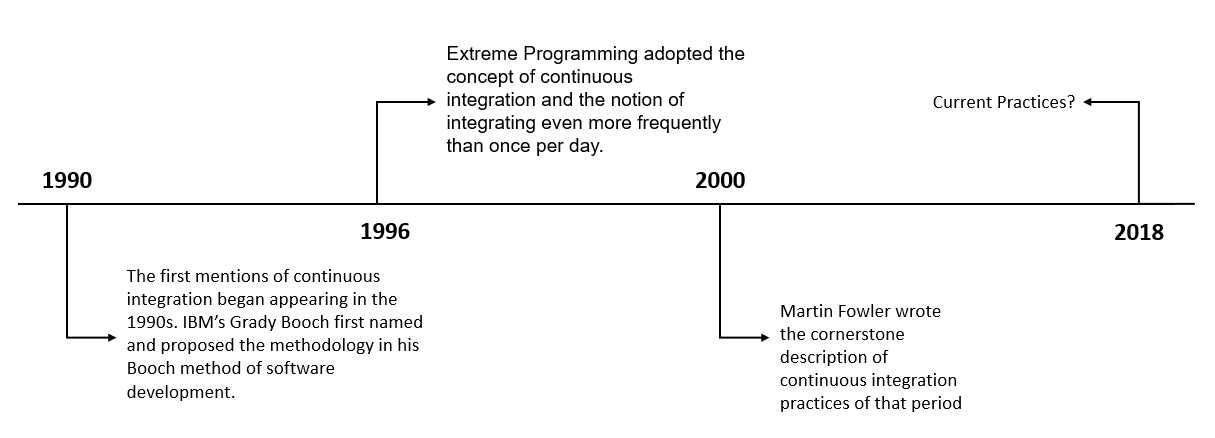
\includegraphics{figures/build-analytics/state_pr.png}
\caption{CI overview.}
\end{figure}

The papers identified using the research protocol defined in section
\ref{build-analytics-research-protocol} that give us an overview of the
current state of the art in build analytics domain are:

\begin{itemize}
\tightlist
\item
  Usage, Costs, and Benefits of Continuous Integration in Open-Source
  Projects {[}\protect\hyperlink{ref-hilton2016usage}{84}{]}
\item
  An Empirical Analysis of Build Failures in the Continuous Integration
  Workflows of Java-Based Open-Source Software
  {[}\protect\hyperlink{ref-rausch2017empirical}{157}{]}
\item
  Continuous Integration
  {[}\protect\hyperlink{ref-fowler2006continuous}{67}{]}
\item
  Enabling Agile Testing Through Continuous Integration
  {[}\protect\hyperlink{ref-stolberg2009enabling}{173}{]}
\item
  Travistorrent: Synthesizing Travis~CI and Github for Full-Stack
  Research on Continuous Integration
  {[}\protect\hyperlink{ref-beller2017travistorrent}{25}{]}
\item
  I'm Leaving You, Travis: A Continuous Integration Breakup Story
  {[}\protect\hyperlink{ref-widder2018m}{190}{]}
\item
  Continuous integration in a social-coding world: Empirical evidence
  from GITHUB {[}\protect\hyperlink{ref-vasilescu2014continuous}{183}{]}
\end{itemize}

The topics that are being explored are:

\begin{itemize}
\tightlist
\item
  Usage of CI in the industry by
  {[}\protect\hyperlink{ref-hilton2016usage}{84}{]}
\item
  Growing popularity of CI due to the introduction of VCS as suggested
  by {[}\protect\hyperlink{ref-rausch2017empirical}{157}{]}
\item
  Common practices used in the industry exemplified by
  {[}\protect\hyperlink{ref-fowler2006continuous}{67}{]}
\item
  Use of common CI practice in the agile approach presented by
  {[}\protect\hyperlink{ref-stolberg2009enabling}{173}{]}
\item
  Comparison between pull requests and direct commits to result in
  successful build as uncovered by
  {[}\protect\hyperlink{ref-vasilescu2014continuous}{183}{]}
\end{itemize}

\subsubsection{Build Analytics Usage}\label{build-analytics-usage}

A survey conducted in open-source projects by Hilton et al.
{[}\protect\hyperlink{ref-hilton2016usage}{84}{]} indicated that 40\% of
all projects used CI. It observed that a median project introduces CI a
year into development. Furthermore, the paper claims that CI is widely
used in practice nowadays. One of many factors contributing to this is
explored by Rausch et al.
{[}\protect\hyperlink{ref-rausch2017empirical}{157}{]}. The growing
popularity of Version Control Systems (VCS) such as GitHub, and hosting
build automation platforms such as Travis have enabled any business of
size to adopt the CI framework. As suggested by Hilton et al.
{[}\protect\hyperlink{ref-hilton2016usage}{84}{]}, the cost and time
associated with introducing the CI framework is not enormous and the
copious benefits far outweigh the resources required.

\subsubsection{Build Analytics
Practices}\label{build-analytics-practices}

The CI concept, often attributed to Martin Fowler
{[}\protect\hyperlink{ref-fowler2006continuous}{67}{]} , is recommended
as best practice of agile software development methods such as extreme
Programming {[}\protect\hyperlink{ref-stolberg2009enabling}{173}{]}. He
introduced many practices that are essential in maintaining the CI
framework. Fowler and Foemmel
{[}\protect\hyperlink{ref-fowler2006continuous}{67}{]} urges engineers
to keep all artifacts required to build the project in a single
repository. This ensures that the system does not require additional
dependencies. In addition, he advises creating a build script that can
compile the code, execute unit tests and automate integration. Once the
code is built, all tests should run to confirm that it behaves as the
developer would expect it to behave. In this way, we are finding and
eradicating software bugs earlier and keeping builds fast. As explored
by Widder et al.{[}\protect\hyperlink{ref-widder2018m}{190}{]}, one of
the factors that lead to companies abandoning the CI framework is the
complexity of the build. A good practice is to have more fast-executing
tests than slow tests.

Furthermore, builds should be readily available to stakeholders and
testers as this can reduce the amount of rework required when rebuilding
a feature that does not meet requirements. In general, all companies
should schedule a ``nightly build'' to update the project from the
repository to ensure everyone is up to date. Continuous Integration is
all about communication, so it is important to ensure that everyone can
easily see the current state of the system. This is also another reason
why CI works well in the agile industry
{[}\protect\hyperlink{ref-stolberg2009enabling}{173}{]}. Both techniques
stress the importance of good communication.

The paper by Vasilescu et al.
{[}\protect\hyperlink{ref-vasilescu2014continuous}{183}{]} studies a
sample of large and active GitHub projects developed in Java, Python and
Ruby. The paper finds that direct code modifications (commits) and more
popular than indirect code modifications (pull request). Additionally,
the notion of automated testing is not as widely practiced. Most samples
in Vasilescu {[}\protect\hyperlink{ref-vasilescu2014continuous}{183}{]}
study were configured to use Travis~CI, however, less than half do. In
terms of languages, Ruby projects are among the early adopters of
Travis~CI, while Java projects are late to adopt CI. The paper uncovers
that the pull requests are much more likely to result in successful
builds than direct commits.

\subsection{Build Analytics Future
Research}\label{build-analytics-future-research}

\textbf{RQ3}: What future research can we expect in the field of build
analytics?

Currently research on build analytics is limited by some challenges,
some are specific to build analytics and some are applicable to the
entire field of software engineering.

The papers identified using the research protocol defined in section
\ref{build-analytics-research-protocol} that give us an overview of
challenges and future research in the field of build analytics are:

\begin{itemize}
\tightlist
\item
  Built to last or built too fast?: evaluating prediction models for
  build times {[}\protect\hyperlink{ref-bisong2017built}{30}{]}
\item
  Work Practices and Challenges in Continuous Integration: A Survey with
  Travis~CI Users {[}\protect\hyperlink{ref-pinto2018work}{146}{]}
\item
  Statically Verifying Continuous Integration Configurations
  {[}\protect\hyperlink{ref-santolucito2018statically}{163}{]}
\item
  (No) Influence of Continuous Integration on the Commit Activity in
  GitHub Projects {[}\protect\hyperlink{ref-baltes2018no}{12}{]}
\item
  The impact of continuous integration on other software development
  practices: a large-scale empirical study
  {[}\protect\hyperlink{ref-zhao2017impact}{196}{]}
\item
  Un-Break My Build: Assisting Developers with Build Repair Hints
  {[}\protect\hyperlink{ref-vassallo2018break}{184}{]}
\item
  Oops, my tests broke the build: An explorative analysis of Travis~CI
  with GitHub {[}\protect\hyperlink{ref-beller2017oops}{24}{]}
\end{itemize}

In Bisong et al.{[}\protect\hyperlink{ref-bisong2017built}{30}{]} the
main limitation was the performance of the machine learning algorithm
used. In the implementation R was used and it proved not capable of
processing the amounts of data needed. This shows that it is important
to choose the right tool when analyzing data.

In Pinto and Rebouças{[}\protect\hyperlink{ref-pinto2018work}{146}{]} it
is noted that research is often done on open source software. There are
still a lot of possibilities for researching on proprietary software
projects.

Tools presented in papers might require a more large-scale and long-term
study to verify that the tool presented keeps up when it is
used{[}\protect\hyperlink{ref-santolucito2018statically}{163}{]}.

Future research in build analytics branches in a couple of different
topics. Pinto and
Rebouças{[}\protect\hyperlink{ref-pinto2018work}{146}{]} proposes to
focus on getting a better understanding of the users and why they might
choose to abandon an automatic build platform.

Baltes et al.{[}\protect\hyperlink{ref-baltes2018no}{12}{]} suggest that
in future research more perspectives when analyzing commit data should
be considered, for instance partitioning commits by developer. It also
notes the importance of more qualitative research.

Some open research questions from recent papers are the following:

\begin{itemize}
\tightlist
\item
  How do teams change their pull request review practices in response to
  the introduction of continuous integration?
  {[}\protect\hyperlink{ref-zhao2017impact}{196}{]}
\item
  How can we detect if fixing a build configuration requires changes in
  the remote environment?
  {[}\protect\hyperlink{ref-vassallo2018break}{184}{]}
\item
  Does breaking the build often translate to worse project quality and
  decreased productivity?
  {[}\protect\hyperlink{ref-beller2017oops}{24}{]}
\item
  Could already trained models on projects with more data available be
  used to make accurate predictions on newer projects with less data
  available? {[}\protect\hyperlink{ref-ni2018acona}{137}{]}
\end{itemize}

From the synthesis of the works discussed in this section the following
research questions emerged:

\begin{itemize}
\tightlist
\item
  What is the impact of the choice of Continuous Integration platform?
  Most of the research is done on users using Travis~CI, there are many
  other platforms out there. Every platform has their own
  characteristics and this could impact the effectiveness for a specific
  kind of project.
\item
  How does the platform or programming language influence effectiveness
  or adoption of continuous integration systems?
\item
  How can machine learning methods be better applied in the field of
  build analytics in order to generate predictions that are easier to
  explain and thus that can be used in practice?
\end{itemize}

\chapter*{Appendix: Build Analytics}\label{appendix-build-analytics}
\addcontentsline{toc}{chapter}{Appendix: Build Analytics}

\begin{longtable}[]{@{}llll@{}}
\caption{\label{tab:build-analytics-selected-papers} Selected
papers}\tabularnewline
\toprule
\begin{minipage}[b]{0.48\columnwidth}\raggedright\strut
Paper with reference\strut
\end{minipage} & \begin{minipage}[b]{0.20\columnwidth}\raggedright\strut
Source\strut
\end{minipage} & \begin{minipage}[b]{0.14\columnwidth}\raggedright\strut
RQ\strut
\end{minipage} & \begin{minipage}[b]{0.06\columnwidth}\raggedright\strut
Notes\strut
\end{minipage}\tabularnewline
\midrule
\endfirsthead
\toprule
\begin{minipage}[b]{0.48\columnwidth}\raggedright\strut
Paper with reference\strut
\end{minipage} & \begin{minipage}[b]{0.20\columnwidth}\raggedright\strut
Source\strut
\end{minipage} & \begin{minipage}[b]{0.14\columnwidth}\raggedright\strut
RQ\strut
\end{minipage} & \begin{minipage}[b]{0.06\columnwidth}\raggedright\strut
Notes\strut
\end{minipage}\tabularnewline
\midrule
\endhead
\begin{minipage}[t]{0.48\columnwidth}\raggedright\strut
1. Bird et al. 2017
{[}\protect\hyperlink{ref-bird2017predicting}{28}{]}\strut
\end{minipage} & \begin{minipage}[t]{0.20\columnwidth}\raggedright\strut
Initial seed\strut
\end{minipage} & \begin{minipage}[t]{0.14\columnwidth}\raggedright\strut
RQ1\strut
\end{minipage} & \begin{minipage}[t]{0.06\columnwidth}\raggedright\strut
1\strut
\end{minipage}\tabularnewline
\begin{minipage}[t]{0.48\columnwidth}\raggedright\strut
2. Beller et al. 2017
{[}\protect\hyperlink{ref-beller2017oops}{24}{]}\strut
\end{minipage} & \begin{minipage}[t]{0.20\columnwidth}\raggedright\strut
Initial seed\strut
\end{minipage} & \begin{minipage}[t]{0.14\columnwidth}\raggedright\strut
RQ3\strut
\end{minipage} & \begin{minipage}[t]{0.06\columnwidth}\raggedright\strut
-\strut
\end{minipage}\tabularnewline
\begin{minipage}[t]{0.48\columnwidth}\raggedright\strut
3. Rausch et al. 2017
{[}\protect\hyperlink{ref-rausch2017empirical}{157}{]}\strut
\end{minipage} & \begin{minipage}[t]{0.20\columnwidth}\raggedright\strut
Initial seed\strut
\end{minipage} & \begin{minipage}[t]{0.14\columnwidth}\raggedright\strut
RQ2\strut
\end{minipage} & \begin{minipage}[t]{0.06\columnwidth}\raggedright\strut
-\strut
\end{minipage}\tabularnewline
\begin{minipage}[t]{0.48\columnwidth}\raggedright\strut
4. Beller et al. TravisTorrent 2017
{[}\protect\hyperlink{ref-beller2017travistorrent}{25}{]}\strut
\end{minipage} & \begin{minipage}[t]{0.20\columnwidth}\raggedright\strut
Initial seed\strut
\end{minipage} & \begin{minipage}[t]{0.14\columnwidth}\raggedright\strut
RQ2\strut
\end{minipage} & \begin{minipage}[t]{0.06\columnwidth}\raggedright\strut
-\strut
\end{minipage}\tabularnewline
\begin{minipage}[t]{0.48\columnwidth}\raggedright\strut
5. Pinto et al. 2018
{[}\protect\hyperlink{ref-pinto2018work}{146}{]}\strut
\end{minipage} & \begin{minipage}[t]{0.20\columnwidth}\raggedright\strut
Initial seed\strut
\end{minipage} & \begin{minipage}[t]{0.14\columnwidth}\raggedright\strut
RQ3\strut
\end{minipage} & \begin{minipage}[t]{0.06\columnwidth}\raggedright\strut
-\strut
\end{minipage}\tabularnewline
\begin{minipage}[t]{0.48\columnwidth}\raggedright\strut
6. Zhao et al. 2017
{[}\protect\hyperlink{ref-zhao2017impact}{196}{]}\strut
\end{minipage} & \begin{minipage}[t]{0.20\columnwidth}\raggedright\strut
Initial seed\strut
\end{minipage} & \begin{minipage}[t]{0.14\columnwidth}\raggedright\strut
RQ3\strut
\end{minipage} & \begin{minipage}[t]{0.06\columnwidth}\raggedright\strut
2\strut
\end{minipage}\tabularnewline
\begin{minipage}[t]{0.48\columnwidth}\raggedright\strut
7. Widder et al. 2018
{[}\protect\hyperlink{ref-widder2018m}{190}{]}\strut
\end{minipage} & \begin{minipage}[t]{0.20\columnwidth}\raggedright\strut
Initial seed\strut
\end{minipage} & \begin{minipage}[t]{0.14\columnwidth}\raggedright\strut
RQ1\strut
\end{minipage} & \begin{minipage}[t]{0.06\columnwidth}\raggedright\strut
-\strut
\end{minipage}\tabularnewline
\begin{minipage}[t]{0.48\columnwidth}\raggedright\strut
8. Hilton et al. 2016
{[}\protect\hyperlink{ref-hilton2016usage}{84}{]}\strut
\end{minipage} & \begin{minipage}[t]{0.20\columnwidth}\raggedright\strut
Initial seed\strut
\end{minipage} & \begin{minipage}[t]{0.14\columnwidth}\raggedright\strut
RQ2\strut
\end{minipage} & \begin{minipage}[t]{0.06\columnwidth}\raggedright\strut
-\strut
\end{minipage}\tabularnewline
\begin{minipage}[t]{0.48\columnwidth}\raggedright\strut
9. Vassallo et al. 2017
{[}\protect\hyperlink{ref-vassallo2017tale}{185}{]}\strut
\end{minipage} & \begin{minipage}[t]{0.20\columnwidth}\raggedright\strut
Ref 2\strut
\end{minipage} & \begin{minipage}[t]{0.14\columnwidth}\raggedright\strut
-\strut
\end{minipage} & \begin{minipage}[t]{0.06\columnwidth}\raggedright\strut
3\strut
\end{minipage}\tabularnewline
\begin{minipage}[t]{0.48\columnwidth}\raggedright\strut
11. Hassan and Wang 2018
{[}\protect\hyperlink{ref-hassan2018hirebuild}{80}{]}\strut
\end{minipage} & \begin{minipage}[t]{0.20\columnwidth}\raggedright\strut
Ref 4\strut
\end{minipage} & \begin{minipage}[t]{0.14\columnwidth}\raggedright\strut
RQ1\strut
\end{minipage} & \begin{minipage}[t]{0.06\columnwidth}\raggedright\strut
-\strut
\end{minipage}\tabularnewline
\begin{minipage}[t]{0.48\columnwidth}\raggedright\strut
12. Vassallo et al. 2018
{[}\protect\hyperlink{ref-vassallo2018break}{184}{]}\strut
\end{minipage} & \begin{minipage}[t]{0.20\columnwidth}\raggedright\strut
Ref 2,3\strut
\end{minipage} & \begin{minipage}[t]{0.14\columnwidth}\raggedright\strut
RQ1, RQ3\strut
\end{minipage} & \begin{minipage}[t]{0.06\columnwidth}\raggedright\strut
-\strut
\end{minipage}\tabularnewline
\begin{minipage}[t]{0.48\columnwidth}\raggedright\strut
13. Zampetti et al. 2017
{[}\protect\hyperlink{ref-zampetti2017open}{194}{]}\strut
\end{minipage} & \begin{minipage}[t]{0.20\columnwidth}\raggedright\strut
Ref by 12\strut
\end{minipage} & \begin{minipage}[t]{0.14\columnwidth}\raggedright\strut
-\strut
\end{minipage} & \begin{minipage}[t]{0.06\columnwidth}\raggedright\strut
3\strut
\end{minipage}\tabularnewline
\begin{minipage}[t]{0.48\columnwidth}\raggedright\strut
14. Baltes et al. 2018
{[}\protect\hyperlink{ref-baltes2018no}{12}{]}\strut
\end{minipage} & \begin{minipage}[t]{0.20\columnwidth}\raggedright\strut
GScholar Search\strut
\end{minipage} & \begin{minipage}[t]{0.14\columnwidth}\raggedright\strut
RQ1, RQ3\strut
\end{minipage} & \begin{minipage}[t]{0.06\columnwidth}\raggedright\strut
4\strut
\end{minipage}\tabularnewline
\begin{minipage}[t]{0.48\columnwidth}\raggedright\strut
15. Bisong et al. 2017
{[}\protect\hyperlink{ref-bisong2017built}{30}{]}\strut
\end{minipage} & \begin{minipage}[t]{0.20\columnwidth}\raggedright\strut
GScholar Search\strut
\end{minipage} & \begin{minipage}[t]{0.14\columnwidth}\raggedright\strut
RQ1, RQ3\strut
\end{minipage} & \begin{minipage}[t]{0.06\columnwidth}\raggedright\strut
5\strut
\end{minipage}\tabularnewline
\begin{minipage}[t]{0.48\columnwidth}\raggedright\strut
16. Santolucito et al. 2018
{[}\protect\hyperlink{ref-santolucito2018statically}{163}{]}\strut
\end{minipage} & \begin{minipage}[t]{0.20\columnwidth}\raggedright\strut
GScholar Search\strut
\end{minipage} & \begin{minipage}[t]{0.14\columnwidth}\raggedright\strut
RQ1\strut
\end{minipage} & \begin{minipage}[t]{0.06\columnwidth}\raggedright\strut
4\strut
\end{minipage}\tabularnewline
\begin{minipage}[t]{0.48\columnwidth}\raggedright\strut
17. Ni and Li 2018 {[}\protect\hyperlink{ref-ni2018acona}{137}{]}\strut
\end{minipage} & \begin{minipage}[t]{0.20\columnwidth}\raggedright\strut
GScholar Search\strut
\end{minipage} & \begin{minipage}[t]{0.14\columnwidth}\raggedright\strut
RQ1\strut
\end{minipage} & \begin{minipage}[t]{0.06\columnwidth}\raggedright\strut
6\strut
\end{minipage}\tabularnewline
\begin{minipage}[t]{0.48\columnwidth}\raggedright\strut
18. Fowler and Foemmel 2006
{[}\protect\hyperlink{ref-fowler2006continuous}{67}{]}\strut
\end{minipage} & \begin{minipage}[t]{0.20\columnwidth}\raggedright\strut
GScholar Search\strut
\end{minipage} & \begin{minipage}[t]{0.14\columnwidth}\raggedright\strut
RQ2\strut
\end{minipage} & \begin{minipage}[t]{0.06\columnwidth}\raggedright\strut
7\strut
\end{minipage}\tabularnewline
\begin{minipage}[t]{0.48\columnwidth}\raggedright\strut
19. Stolberg 2009
{[}\protect\hyperlink{ref-stolberg2009enabling}{173}{]}\strut
\end{minipage} & \begin{minipage}[t]{0.20\columnwidth}\raggedright\strut
GScholar Search\strut
\end{minipage} & \begin{minipage}[t]{0.14\columnwidth}\raggedright\strut
RQ2\strut
\end{minipage} & \begin{minipage}[t]{0.06\columnwidth}\raggedright\strut
7\strut
\end{minipage}\tabularnewline
\begin{minipage}[t]{0.48\columnwidth}\raggedright\strut
20. Vasilescu et al. 2014
{[}\protect\hyperlink{ref-vasilescu2014continuous}{183}{]}\strut
\end{minipage} & \begin{minipage}[t]{0.20\columnwidth}\raggedright\strut
GScholar Search\strut
\end{minipage} & \begin{minipage}[t]{0.14\columnwidth}\raggedright\strut
RQ2\strut
\end{minipage} & \begin{minipage}[t]{0.06\columnwidth}\raggedright\strut
7\strut
\end{minipage}\tabularnewline
\bottomrule
\end{longtable}

\textbf{Notes}

\begin{enumerate}
\def\labelenumi{\arabic{enumi}.}
\tightlist
\item
  US patent owned by Microsoft.
\item
  Collaboration between universities in China, The Netherlands and The
  USA.
\item
  Not included in this survey as it did not introduce a new technique or
  practice.
\item
  Using search term ``Github Continuous Integration''.
\item
  Using search term ``Predicting build time''
\item
  Using search term ``Predicting build failures''
\item
  Using search term ``Current practices in Continuous Integration''
\end{enumerate}

\chapter{Bug Prediction}\label{bug-prediction}

\section{Motivation}\label{motivation-2}

Minimizing the number of bugs in software is an effort central to
software engineering --- faulty code fails to fulfill the purpose it was
written for, its impact ranges from slightly embarrassing to disastrous
and dangerous, and last but not least --- fixing it costs time and
money. Resources in a software development life cycle are almost always
limited and therefore should be allocated to where they are needed most
--- in order to avoid bugs, they should be focused on the most
fault-prone areas of the project. Being able to predict where such areas
might be would allow more development and testing efforts to be
allocated on the right places.

However, reliably predicting which parts of source code are the most
fault-prone is one of the holy grails of software engineering
{[}\protect\hyperlink{ref-DAmbros2012}{64}{]}. Thus it is not surprising
that bug prediction continues to garner a widespread research interest
in software analytics, now equipped with the ever-expanding toolbox of
data-mining and machine learning techniques. In this survey we
investigate the current efforts in bug prediction in the light of the
advances in software analytics methods and focus our attention on
answering the following research questions:

\begin{itemize}
\tightlist
\item
  \textbf{RQ1} What is the current state of the art in bug prediction?
  More specifically, we aim to answer the following:

  \begin{itemize}
  \tightlist
  \item
    What software or other metrics does bug prediction models rely on
    and how good are they?
  \item
    What kind prediction models are predominantly used?
  \item
    How are bug prediction models and results validated and evaluated?
  \end{itemize}
\item
  \textbf{RQ2} What is the current state of practice in bug prediction?

  \begin{itemize}
  \tightlist
  \item
    Are bug prediction techniques applied in practice and if so, how?
  \item
    Are the current developments in the field able to provide actionable
    tools for developers?
  \end{itemize}
\item
  \textbf{RQ3} What are some of the open challenges and directions for
  future research?
\end{itemize}

\section{Research protocol}\label{research-protocol-1}

We started by studying the initial 6 seed papers which were selected
based on domain knowledge:

\begin{longtable}[]{@{}lll@{}}
\toprule
\begin{minipage}[b]{0.23\columnwidth}\raggedright\strut
Reference\strut
\end{minipage} & \begin{minipage}[b]{0.18\columnwidth}\raggedright\strut
Topic\strut
\end{minipage} & \begin{minipage}[b]{0.50\columnwidth}\raggedright\strut
Summary\strut
\end{minipage}\tabularnewline
\midrule
\endhead
\begin{minipage}[t]{0.23\columnwidth}\raggedright\strut
{[}\protect\hyperlink{ref-Gyimothy2005}{76}{]}\strut
\end{minipage} & \begin{minipage}[t]{0.18\columnwidth}\raggedright\strut
metrics validation\strut
\end{minipage} & \begin{minipage}[t]{0.50\columnwidth}\raggedright\strut
performance of object-oriented metrics\strut
\end{minipage}\tabularnewline
\begin{minipage}[t]{0.23\columnwidth}\raggedright\strut
{[}\protect\hyperlink{ref-Catal2009review}{38}{]}\strut
\end{minipage} & \begin{minipage}[t]{0.18\columnwidth}\raggedright\strut
literature review\strut
\end{minipage} & \begin{minipage}[t]{0.50\columnwidth}\raggedright\strut
comparison of metrics, methods, datasets\strut
\end{minipage}\tabularnewline
\begin{minipage}[t]{0.23\columnwidth}\raggedright\strut
{[}\protect\hyperlink{ref-Arisholm2010}{9}{]}\strut
\end{minipage} & \begin{minipage}[t]{0.18\columnwidth}\raggedright\strut
literature review\strut
\end{minipage} & \begin{minipage}[t]{0.50\columnwidth}\raggedright\strut
comparison of models, metrics, performance measures\strut
\end{minipage}\tabularnewline
\begin{minipage}[t]{0.23\columnwidth}\raggedright\strut
{[}\protect\hyperlink{ref-DAmbros2010}{63}{]}\strut
\end{minipage} & \begin{minipage}[t]{0.18\columnwidth}\raggedright\strut
BP performance\strut
\end{minipage} & \begin{minipage}[t]{0.50\columnwidth}\raggedright\strut
benchmark for bug prediction, evaluation of approaches using the
benchmark\strut
\end{minipage}\tabularnewline
\begin{minipage}[t]{0.23\columnwidth}\raggedright\strut
{[}\protect\hyperlink{ref-Hall2012}{77}{]}\strut
\end{minipage} & \begin{minipage}[t]{0.18\columnwidth}\raggedright\strut
literature review\strut
\end{minipage} & \begin{minipage}[t]{0.50\columnwidth}\raggedright\strut
influence of model context, methods, metrics on performance\strut
\end{minipage}\tabularnewline
\begin{minipage}[t]{0.23\columnwidth}\raggedright\strut
{[}\protect\hyperlink{ref-Lewis2013}{110}{]}\strut
\end{minipage} & \begin{minipage}[t]{0.18\columnwidth}\raggedright\strut
case study\strut
\end{minipage} & \begin{minipage}[t]{0.50\columnwidth}\raggedright\strut
BP deployment in industry\strut
\end{minipage}\tabularnewline
\bottomrule
\end{longtable}

We looked for additional papers with the following queries:

\begin{enumerate}
\def\labelenumi{\arabic{enumi}.}
\item
  Keyword search using search engines (Google Scholar, Scopus, ACM
  Digital Library, IEEE Explorer). The search query was constructed so
  that the paper had to contain the phrase bug prediction, but also the
  other more general variants used in literature: \emph{bug/defect/fault
  prediction}. The paper also had to contain at least one of following
  keywords: \emph{metrics}, \emph{models}, \emph{validation},
  \emph{evaluation}, \emph{developers}.
\item
  Filtering search results by publication date. We narrow the scope to
  \emph{recent} papers, which we define as ``published within the last
  10 years'' for the purposes of this review. Therefore we excluded
  papers published before 2008. However, there were a few exceptions for
  papers which had very high impact.
\item
  Filtering by the number of citations. We selected papers with 10 or
  more citations in order to focus on the ones that already have some
  visibility within the field. Also, there were some exceptions for
  every recently published papers.
\item
  Exploring other impactful publications by the same authors.
\end{enumerate}

The papers chosen had to fulfill the above criteria.

\emph{Table 2. Papers found by investigating the authors of other
papers.}

\begin{longtable}[]{@{}lll@{}}
\toprule
Starting paper & Relationship & Result\tabularnewline
\midrule
\endhead
{[}\protect\hyperlink{ref-DAmbros2010}{63}{]} & is author of &
{[}\protect\hyperlink{ref-DAmbros2012}{64}{]}\tabularnewline
{[}\protect\hyperlink{ref-Catal2009review}{38}{]} & is author of &
{[}\protect\hyperlink{ref-Catal2011}{37}{]}
{[}\protect\hyperlink{ref-Catal2009investigating}{39}{]}\tabularnewline
{[}\protect\hyperlink{ref-rahman2011}{155}{]} & is author of &
{[}\protect\hyperlink{ref-Rahman2013}{154}{]}\tabularnewline
{[}\protect\hyperlink{ref-Giger2011}{73}{]} & is author of &
{[}\protect\hyperlink{ref-giger2012}{72}{]}\tabularnewline
\bottomrule
\end{longtable}

\section{Answers}\label{answers-1}

\subsection{RQ1: Metrics}\label{rq1-metrics}

To find out what metrics are commonly used to build bug prediction
models, we studied the papers that either focus their entirety or at
least a section to the discussion of software metrics used for bug
prediction. Based on the results and observations made in the relevant
studies, we classify the software metrics most commonly used in two
groups based on which aspect of a piece of software they measure:

\begin{itemize}
\tightlist
\item
  \emph{The product}: the (static) code itself.
\item
  \emph{The process}: the different aspects that describe how the
  product developed through time. We include both simpler changelog
  based metrics that require different versions as well as metrics that
  require detailed process recording.
\end{itemize}

\subsubsection{Product metrics}\label{product-metrics}

Different metrics incur different costs based on whether they require
additional efforts in order to collect data and setup an instrumentation
infrastructure. Measuring various aspects of what is already available
--- a snapshot of source code --- is an obvious starting point when
building a set of predictive features and it turns out code metrics were
the most commonly studied metrics in literature
{[}\protect\hyperlink{ref-Catal2009review}{38}{]}. Traditionally,
examples of metrics obtained by static analysis include \emph{lines of
code} (LOC) as well as \emph{code complexity} (for example, McCabe and
Halstead complexities), with the latter applicable for languages with a
structured control flow and the concept of methods. The rationale behind
using code complexity as a metric for bug prediction is that if code is
complex, it is difficult to change and is therefore bug-prone
{[}\protect\hyperlink{ref-DAmbros2012}{64}{]}.

Another group of more language specific metrics which became popular
after 1990 are the \emph{object-oriented} or \emph{class} metrics which
are based on the idea of classes and measure class-related concepts like
\emph{amount of methods}, \emph{coupling}, \emph{inheritance} and
\emph{cohesion} {[}\protect\hyperlink{ref-Gyimothy2005}{76}{]}.

A drawback of static code metrics is that, the authors find that such
metrics have high stasis which means they do not change a lot from
release to release {[}\protect\hyperlink{ref-Rahman2013}{154}{]}. In
turn, this can cause stagnation in the prediction models, which classify
the same files as bug-prone over and over.

\subsubsection{Process metrics}\label{process-metrics}

The other prominent group of metrics are the process metrics which are
related to the software development process and the changes of the
software through time. Additional infrastructure has to be in place in
order to capture the process features and typically at least a version
control system is required. One of the rationales behind using these
metric in a predictive model is that bugs are introduced by changes in
software and should be studied
{[}\protect\hyperlink{ref-DAmbros2012}{64}{]}.

Some examples of process metrics include \emph{code churn}, \emph{number
of revisions}, \emph{active developer count}, \emph{distinct developer
count}, \emph{changed code scattering}, \emph{average lines of code
added per revision} and \emph{age of a file}
{[}\protect\hyperlink{ref-Moser2008}{134}{]}. There are also metrics
based on \emph{prior faults}, that argue files which in the past
contained faults will probably have more faults in the future. It is
shown that predictors based on previous bugs show better results than
predictors based on code changes
{[}\protect\hyperlink{ref-rahman2011}{155}{]}.

Other metrics are derived by looking at the source code change history
as either \emph{delta metrics} or \emph{code churn}
{[}\protect\hyperlink{ref-Radjenovic2013}{152}{]}. Delta metrics are not
separate new metrics per se, but are derived from other metrics by
comparing versions of software to each other.

Some studies found that process metrics outperform code metrics by
comparing prediction results of both metrics
{[}\protect\hyperlink{ref-Moser2008}{134}{]}. It was also shown that
process metrics are more stable across releases
{[}\protect\hyperlink{ref-Rahman2013}{154}{]}. However, note that such
results should be taken with a grain of salt; it was found that when
comparing a selection of representative bug prediction approaches, the
results considering metrics highly depend on the choice of learner and
could not necessarily be generalized
{[}\protect\hyperlink{ref-DAmbros2012}{64}{]}.

There are potential advantages of using more fine-grained source code
changes, capturing them at statement level and including the changes'
semantics {[}\protect\hyperlink{ref-Giger2011}{73}{]}. This data can be
obtained by building abstract syntax trees (ASTs) and using the changes
required to transform one AST to the other as metrics. These models were
found to outperform models based on other coarser metrics such as code
churn; however, the gain in performance comes at the cost of extracting
these fine-grained changes.

\paragraph{Developer-based metrics}\label{developer-based-metrics}

Besides metrics from code repositories we can also extract some metrics
from developers itself. It was shown that modules touched by more
developers are more likely to contain more bugs
{[}\protect\hyperlink{ref-Matsumoto2010}{122}{]}. Also, using developer
based metrics in combination with other metrics can improve prediction
results {[}\protect\hyperlink{ref-Matsumoto2010}{122}{]}. Furthermore,
it turns out that developer experience has no clear correlation with how
much faults they introduce
{[}\protect\hyperlink{ref-rahman2011}{155}{]}.

Faults can also be predicted by tracking micro-interactions of
developers {[}\protect\hyperlink{ref-Lee2011}{107}{]}. The authors find
that the most informative metrics are the \emph{number of
low-degree-of-interest-file editing events}, \emph{editing and selecting
bug-prone files consecutively}, and \emph{time spent on editing}. They
find that their prediction results exceed those of some product and
process metrics.

Another set of metrics are scattering metrics, which uses data about how
focussed a developers work is
{[}\protect\hyperlink{ref-DiNucci2018}{55}{]}. Structural scattering
describes how structurally far apart in the project the code is.
Semantic scattering measures how different the code being edited is in
terms of implemented responsibilities, this is measured by textually
comparing the code. The authors find they have relatively high accuracy
and perform better than a baseline selection of code and process
metrics.

\subsection{RQ1: Models}\label{rq1-models}

In the section above we have seen different kinds of metrics, in this
section we will show how these metrics are used to create models for bug
prediction which can actually be used. We will also show some
preliminary results of these models, however, as we will explain later
on, it is not trivial to compare the results of different models.

\paragraph{\texorpdfstring{History Complexity Metric
{[}\protect\hyperlink{ref-hassan2009}{79}{]}}{History Complexity Metric {[}79{]}}}\label{history-complexity-metric-hassan2009}

Files that are modified during periods of high change complexity will
contain more faults. Developers changing code during these periods will
make mistakes, because they probably will not be aware of the current
state of the code. This method is useful in practice because companies
may not have a full bug history, while they probably do have history of
code changes. Outperforms models based on prior faults, 15-38\% decrease
in prediction errors. However, D'Ambros et al. contradict this statement
{[}\protect\hyperlink{ref-DAmbros2010}{63}{]}.

\paragraph{\texorpdfstring{FixCache
{[}\protect\hyperlink{ref-kim2007}{100}{]}}{FixCache {[}100{]}}}\label{fixcache-kim2007}

Maintains a fixed-size cache of files that are most likely to contain
bugs. Files are added to cache if it meets one of the locality criteria,
which are:

\begin{itemize}
\tightlist
\item
  Churn locality: if a file is recently modified it is likely to contain
  faults
\item
  Temporal locality: if a file contains a fault, it is more likely to
  contain more faults
\item
  Spatial locality: files that change alongside faulty files are more
  likely to contain faults
\end{itemize}

If the cache if full the least recently used file is removed from the
cache. The size of the cache is set at 10\% of all files. Hit rate of
about 73-95\% at file level, 46-72\% at method level.

\paragraph{\texorpdfstring{Rahman
{[}\protect\hyperlink{ref-rahman2011}{155}{]}}{Rahman {[}155{]}}}\label{rahman-rahman2011}

The Rahman algorithm is based on the FixCache algorithm, in their
research they found that the temporal locality was by far the most
influential factor. The Rahman algorithm is thus implemented based
solely on that factor.

\paragraph{\texorpdfstring{Time-weighted risk algorithm
{[}\protect\hyperlink{ref-Lewis2013}{110}{]}}{Time-weighted risk algorithm {[}110{]}}}\label{time-weighted-risk-algorithm-lewis2013}

An algorithm based on the Rahman algorithm, it includes a weight factor
based on how old a commit is, older bug fixing commits have less impact
on the overall bug-proneness of the file. Instead of showing top 10\% of
bug-prone files, this shows the top 20 files.

\paragraph{Machine learning}\label{machine-learning}

With machine learning methods bugs can be predicted by software tools,
these tools train on the code base, code history and other data from
software repositories. Downside is that these methods give little
insights in why a component is bug-prone
{[}\protect\hyperlink{ref-Lewis2013}{110}{]}. Another downside is that
this does not work for new projects since cross-project defect
prediction does not yet give good results
{[}\protect\hyperlink{ref-zimmermann2009}{197}{]}.

\paragraph{Analysis on Abstract Syntax
Trees}\label{analysis-on-abstract-syntax-trees}

Because ASTs give a more high-level description of the syntax of a
program it could give more useful insights for bug prediction than other
analysis methods. Downside is that ASTs is that dynamic programming
languages cannot produce static ASTs. Wang et al. uses ASTs in
combination with a machine learning approach for bug prediction. They
also show that using ASTs can improve cross-project prediction results
{[}\protect\hyperlink{ref-wang2016}{188}{]}.

\subsection{RQ1: Evaluations}\label{rq1-evaluations}

In order to answer this questions we looked at the scientific papers
that benchmark prediction models in any way, and specifically looked at
the way these are evaluated. We found that most papers use a simple yet
logical approach to benchmark an algorithm's performance. This approach
is called Area Under the Curve (commonly referred as AUC), it consists
of measuring the area under a curve which is known as Receiver Operating
Characteristic (ROC). This process graphically draws the relationship
between the accuracy, which is the ability of an algorithm to find all
existing bug-prone files, and precision, which is how accurate the
algorithm is at finding them (optimal would be no false negatives)
{[}\protect\hyperlink{ref-DAmbros2012}{64}{]}.

Other authors use different methodologies in order to rank the
algorithm's performance. Jiang et al. focuses solely on how to evaluate
the algorithm's performance, and the researchers used the accuracy and
precision metrics in numerical and graphical form, but they also bring
to the table a graphic that helps identify where to spend the project
resources in order to get a greater software quality
{[}\protect\hyperlink{ref-Jiang2008}{91}{]}. Finally, another method is
to use linear regression in order to qualify the fault prediction
method's prediction power {[}\protect\hyperlink{ref-DAmbros2010}{63}{]}.

In conclusion, we can see that the most used methodology is AUC, this is
because, citing Lessman et al.: ``The AUC was recommended as the primary
accuracy indicator for comparative studies in software defect prediction
since it separates predictive performance from class and cost
distributions, which are project-specific characteristics that may be
unknown or subject to change.''
{[}\protect\hyperlink{ref-Lessman2008}{108}{]}.

It is also worth noting the conclusion of Shepperd et al., in which they
found that 30 percent of the variance of the algorithm's performance can
be ``explained'' based on the research group, while the variability due
to the choice of classifier is very small
{[}\protect\hyperlink{ref-Shepperd2014}{167}{]}.

\subsection{RQ2: Practical usage}\label{rq2-practical-usage}

There seems to be none to very little usage of bug prediction tools in
the industry, even searching outside the scope of the scientific
literature did not come up with anything. On GitHub we could only find a
handful of repositories which implement a bug prediction tool, however,
none of these are actively maintained any longer.

Furthermore, all the tools we did find were based on references
{[}\protect\hyperlink{ref-Lewis2013}{110}{]} or
{[}\protect\hyperlink{ref-rahman2011}{155}{]}. Lewis et al. even
mentions that their tool had no significant effect on developers
{[}\protect\hyperlink{ref-Lewis2013}{110}{]}. Kim et al. says software
managers could use a list of bug-prone files to allocate more quality
assurance in some parts of the code, but again, no industry usage could
be found {[}\protect\hyperlink{ref-kim2007}{100}{]}.

We did find some reasons which could explain why there is no practical
usage of bug prediction yet. Some issues we found with using bug
prediction tools in practice have to do with the following properties
that bug prediction tools should have in some cases:

\begin{itemize}
\tightlist
\item
  \emph{Obvious reasoning}: If a tool has no clear reasoning users might
  quickly discard the tool, because they do not understand why a file is
  bug-prone {[}\protect\hyperlink{ref-Lewis2013}{110}{]}.
\item
  \emph{Bias towards the new}: For some metrics this feature is
  required, because otherwise it would be impossible to `fix' a file, it
  will remain to be bug-prone even if completely rewritten
  {[}\protect\hyperlink{ref-Lewis2013}{110}{]}.
\item
  \emph{Actionable messages}: Messages shown by bug prediction tools
  must be actionable. The user must be able to perform an action to fix
  the problem with the file, otherwise users will not know what to do
  with the tool {[}\protect\hyperlink{ref-Lewis2013}{110}{]}.
\item
  \emph{Noise problem}: It turns out that if data which is used for the
  historical changes contains noise this has a large impact on the
  performance of the model. Since the data is mostly mined from software
  repositories this will contain noise
  {[}\protect\hyperlink{ref-Kim2011}{99}{]}.
\item
  \emph{Granularity}: Most methods we found work on a class- or
  file-based granularity, having a lower level of granularity could
  improve the usefulness of the prediction for developers
  {[}\protect\hyperlink{ref-giger2012}{72}{]}.
\end{itemize}

\subsection{RQ2: Actionable tools for
developers}\label{rq2-actionable-tools-for-developers}

The only paper that tackles this question is by Lewis et al., in which
the authors deploy bug predicting software to developers workspaces and
evaluate developers behaviour after and before having the software
{[}\protect\hyperlink{ref-Lewis2013}{110}{]}. In this study they
conclude currently, fault prediction does not provide actionable tools
for developers.

To answer this questions we found no more information in scientific
papers, so we had to look outside of the academic world in order to see
if this techniques are being used by developers. After some research we
concluded that bug prediction is not currently being used on developers,
and we, as in reference {[}\protect\hyperlink{ref-Lewis2013}{110}{]},
think that maybe bug prediction is supposed to be used for software
quality in order to find the places where we should invest the project
resources instead of helping developers write code without bugs.

\subsection{RQ3: Open challenges and future
work}\label{rq3-open-challenges-and-future-work}

We believe that the bug prediction field still has a lot of open
challenges, for example, the use of developer-related factors in the
predictions. Still no strong conclusions have been found, so this field
requires a lot of further investigation to be able to find better models
and useful applications of this techniques. All this challenges are
anchored to a very hard to prove external validity.

In conclusion, bug prediction is still a partially explored area, and
even though some algorithms have proven to be successful to some degree,
we still lack more evidence and more reliable algorithms so they can be
applied in the real world.

\chapter{Ecosystem Analytics}\label{ecosystem-analytics}

\section{Motivation}\label{motivation-3}

In the modern day and age, it is popular to make use of external
software or libraries in software projects to use the functionality (for
example parsing JSON) of these libraries, without having to develop this
functionality itself. For example, in 2016, the package manager npm
recorded 18 billion package downloads in one month, according to
{[}\protect\hyperlink{ref-Linux2016}{171}{]}. Moreover, multiple
languages, such as Python and Rust, provide package managers
(pip\footnote{\url{https://pypi.org/project/pip/}} and Cargo\footnote{\url{https://crates.io/}}
respectively) which can be used to easily manage this third-party
functionality, as well as distribute it.

In parallel to this, the popularity of creating open source projects is
on the rise as well. At the package repository npm only, 4,685 libraries
were added in one week in 2016, according to
{[}\protect\hyperlink{ref-Linux2016}{171}{]}. On platforms such as
GitHub\footnote{\url{https://github.com}}, it is easy and quick to
create a new software project, which can be developed, reviewed and used
by the whole community. This development leads to more libraries being
developed and being available for public use.

As a result of these two developments, software projects are
increasingly becoming interdependent on each other. Inspecting the
dependency relations between projects leads to a graph-like structure of
software projects. In this structure,the nodes are the projects and the
edges represent a dependency between two software projects. This
structure is known as a \emph{software ecosystem}. Messerschmitt and
Szyperski in {[}\protect\hyperlink{ref-Messerschmitt2003}{131}{]} state
that a \emph{software ecosystem} is ``a collection of software products
that have some given degree of symbiotic relationships.'' Another,
similar definition is given by Lungu in
{[}\protect\hyperlink{ref-Lungu2009}{115}{]}: ``A software ecosystem is
a collection of software projects which are developed and co-evolve in
the same environment.'' Mens et al. in
{[}\protect\hyperlink{ref-Mens2013}{130}{]} extend this definition, ``by
explicitly considering the communities involved (e.g.~user and developer
communities) as being part of the software ecosystem.'' Stallman in
{[}\protect\hyperlink{ref-Stallman2002}{170}{]} opposes the overall
notion of calling this structure a software ecosystem: ``It is
inadvisable to describe the free software community, or any human
community, as an ecosystem, because that word implies the absence of
ethical judgment.''

Although Stallman in {[}\protect\hyperlink{ref-Stallman2002}{170}{]}
disagrees with the use of the term ecosystem, he does not necessarily
disagree with the definition of the term. The definition which will be
used in this chapter is the definition of Mens et al. in
{[}\protect\hyperlink{ref-Mens2013}{130}{]}, since it captures the
essence of the other two definitions, while adding the notion of the
human communities alongside as well.

By performing analysis on these software ecosystems, the aim is to
generate meaningful insights. These insights can then be used to improve
the efficiency and effectivity of the software development process, as
well as to learn to identify and inform about potential problems. For
example, a warning could be displayed if a dependency has a security
vulnerability.

The field of research on software ecosystems, \emph{ecosystem
analytics}, focuses on performing such analysis. This chapter discovers
what the current progress is in this field of research through a
literature survey. This discovery is not limited to the theoretical
perspective, but will uncover practical implications as well as the open
challenges of the field. In order to describe each covered aspect, we
have formulated three research questions:

\begin{itemize}
\tightlist
\item
  \textbf{RQ1}: What is the current state of the art in software
  analytics for ecosystem analytics?
\item
  \textbf{RQ2}: What are the practical implications of the state of the
  art?
\item
  \textbf{RQ3}: What are the open challenges in ecosystem analytics, for
  which future research is required?
\end{itemize}

Each of these research questions will be answered using recent papers
written in this field of research.

This chapter is structured as follows. First, the research protocol is
described in detail. This includes decisions on which papers are
included in the review. After this, the research questions are answered
using the previously stated set of papers.

\section{Research Protocol}\label{research-protocol-2}

In order to review literature to answer the research questions given in
the previous section, the survey method suggested by Kitchenham is used,
conform to {[}\protect\hyperlink{ref-kitchenham2004procedures}{102}{]}.
This method creates a systematic way to select a set of papers, which is
relevant to the research question(s).

The search strategy, as described by Kitchenham
{[}\protect\hyperlink{ref-kitchenham2004procedures}{102}{]}, are usually
iterative and benefit from consultations with experts in the field,
among other things. Our search strategy can be split in three different
types:

\begin{itemize}
\tightlist
\item
  the initial seed, given by an expert in the field, MSc. Joseph
  Hejderup
\item
  a search using a digital search engine, namely Google
  Scholar\footnote{\url{https://scholar.google.com}}
\item
  a selection of referenced papers within papers selected before in the
  above two searches
\end{itemize}

\subsection{Initial seed}\label{initial-seed}

MSc. Joseph Hejderup has provided us with a total of thirteen papers, as
shown in Table 4.1.

As each of these papers come from an expert in the field, each paper is
assumed to be relevant to at least the field of software ecosystems.
Because of this, each of these papers were judged on their relevance to
either of the research questions. In Table 4.1, this relevance judgment
is shown in the left column, since a paper is only selected, if the
paper is indeed relevant. Table 4.2 describes the reason for which each
particular paper is not selected for the literature survey.

\subsection{Digital Search Engine}\label{digital-search-engine}

The second strategy type which is used to select relevant papers for
this literature study, is by a digital search engine. In this literature
survey, Google Scholar\footnote{\url{https://scholar.google.com}} is
used. From the initial seed, common keywords were retrieved and the
following queries have been used to search for relevant papers:

\begin{itemize}
\tightlist
\item
  ``engineering software ecosystems'' \emph{(2014)}
\item
  ``software ecosystems'' AND ``empirical analysis'' \emph{(2018)}
\item
  ``software ecosystem'' AND ``empirical'' \emph{(2014)}
\item
  ``software ecosystem analytics'' \emph{(2014)}
\item
  ``software ecosystem'' AND ``analysis'' \emph{(2017)}
\end{itemize}

For each of these queries, the results were first filtered by the
publish year. These are described by the italic year after each query
above. The papers that are filtered are published earlier than the set
publish year. These specific years were chosen since the survey focuses
on the state of the art within the ecosystem analytics. The difference
in years per query is a result from not finding relevant papers in more
recent times (e.g.~for ``software ecosystem analytics'', the year is
\emph{2014} because setting the filter to \emph{2018} or \emph{2017} did
not result in relevant papers).

After this filtering, we first determined whether a paper was relevant
to the literature survey by examining the title. If it was unclear
whether the paper was indeed relevant by only looking at the title, the
abstract of the paper was examined closely. On these two criteria, each
of the selected papers were judged and ultimately selected. The selected
paper using these method can be found in Table 4.3.

\subsection{Referenced papers}\label{referenced-papers}

The third method we use is by looking at the references found in the
selected papers, using the two methods above. A selection has been made
from these references. For these papers, the selection process is
similar to that of the selected papers using the digital search engine;
it is selected when both the title and the abstract are deemed relevant
to the research questions. This has led to the papers in Table 4.4.
being selected.

\section{Answers}\label{answers-2}

In this section, an aggregation of information, found in the papers, is
presented. Each subsection of this section focuses on one of the three
research questions posed in Section 1.

\subsection{RQ1: What is the current state of the art in software
analytics for ecosystem
analytics?}\label{rq1-what-is-the-current-state-of-the-art-in-software-analytics-for-ecosystem-analytics}

To answer this research question, we examine the explored topics in
ecosystem analytics. Moreover, we summarize which research methods,
tools and datasets are being used to explore this topics.

\subsubsection{Explored Topics}\label{explored-topics}

The main topics we explored in ecosystem analytics are the usage of
trivial packages, (breaking) changes in dependencies and their impacts,
quality of dependencies and dependency networks.

Trivial packages are a recurring topic in the area of software
analytics, notably incidents like Left-pad, Schleuter
{[}\protect\hyperlink{ref-NPM2016}{176}{]}, stress the possible impact
trivial packages can have on a software ecosystem. Research in this
topic explores the usage of trivial packages both quantitatively and
qualitatively by analysing the usage of the trivial packages and the
reasons why developers choose to use them respectively.

Breaking changes is a major topic researched by some papers. Much like
trivial packages research is done both quantitatively and qualitatively
in this topic. The impact of breaking changes and the way in which
developers react to these changes are considered to be the notable
problems in this topic.

Establishing a metric for the health of an ecosystem dependency is also
a heavily explored topic. Researchers are trying to find ways in which a
metric can be used to establish the quality of dependencies.

Dependency networks allow us to gain insight in the way in which
ecosystems evolve over time.

\subsubsection{Used Research Methods}\label{used-research-methods}

The studied papers cover a plethora of research methods. These methods
can be divided into two categories: quantitative and qualitative.

Many quantitative research papers analyse the data in a statistical
manner, using software ecosystems as their data. The types of data
depend heavily on the ecosystem used for analysis. Some papers go as far
as using the source code of packages
{[}\protect\hyperlink{ref-Abdalkareem2017}{3}{]}. While other research
focusses on the meta-data of software ecosystems, such as dependency
networks {[}\protect\hyperlink{ref-Kikas2017}{97}{]}. Another recurring
research method is survival analysis, as used by
{[}\protect\hyperlink{ref-Decan2018}{54}{]}, which can be used to
estimate the survival rate of a population over time. In software
engineering this has been successfully applied to open source projects.

Some qualitative research has been done in software ecosystems to gain a
better understanding in to the behaviour of the interactions between
developers and software ecosystems. Some papers solely rely on the
results of qualitative research whereas some papers use both
quantitative research and qualitative research to triangulate their
findings.

\subsubsection{Used Ecosystems}\label{used-ecosystems}

As has been said above, the most common explored topic within the body
of studied papers are topics relating to dependencies between different
software projects. Therefore, it does make a lot of sense that the most
common ecosystems used are those of package managers, since these
package managers are central repositories from which the packages, as
well as their dependencies, can easily be retrieved.

The most common used ecosystem in the studied papers is
\emph{npm}\footnote{\url{https://npmjs.com}}, as used by Abdalkareem et
al. {[}\protect\hyperlink{ref-Abdalkareem2017}{3}{]}, Bogart et al.
{[}\protect\hyperlink{ref-Bogart2016}{32}{]}, Decan, Mens, and Claes
{[}\protect\hyperlink{ref-Decan2017}{53}{]}, Kikas et al.
{[}\protect\hyperlink{ref-Kikas2017}{97}{]}, and Decan, Mens and
Grosjean {[}\protect\hyperlink{ref-Decan2018}{54}{]}. There are a few
reasons why this is the most common used ecosystem throughout the
papers. Firstly, npm is the largest software registry, containing more
than double of the next most populated package registry in 2016
{[}\protect\hyperlink{ref-Linux2016}{171}{]}. Moreover, npm is the
package manager of JavaScript, which is the most used programming
language according to a RedMonk survey
{[}\protect\hyperlink{ref-RedMonk2018}{177}{]}. Kikas et al.
{[}\protect\hyperlink{ref-Kikas2017}{97}{]} explain that it is
beneficial to use this ecosystem, because the majority of their packages
are hosted on GitHub and Developers specify required packages in their
project's dependency files. There are more ecosystems which have the
same properties, such as RubyGems (Ruby) and Crates.io (Rust)
{[}\protect\hyperlink{ref-Kikas2017}{97}{]}.

However, these are not the only used ecosystems. Decan, Mens, and
Grosjean {[}\protect\hyperlink{ref-Decan2018}{54}{]} use the
\emph{libraries.io} dataset for their research, which includes seven
different packaging ecosystems: Cargo (rust), CPAN (Perl), CRAN (R), npm
(JavaScript), NuGet (.NET), Packagist (PHP) and RubyGems (Ruby). Decan,
Mens, and Grosjean {[}\protect\hyperlink{ref-Decan2018}{54}{]} therefore
study the most different ecosystems in one paper, relative to the papers
studied in this survey.

Apart from these datasets based on packages in package repositories,
there are papers which use other datasets and therefore ecosystems as
well. Bavota et al. {[}\protect\hyperlink{ref-Bavota2014}{17}{]}
research the Apache Community and therefore uses a dataset corresponding
to the full Java subset of the Apache ecosystem. Cox et al.
{[}\protect\hyperlink{ref-Cox2015}{49}{]} instead use the dataset of the
Apache Maven Project to validate his created metric. Claes et al.
{[}\protect\hyperlink{ref-Claes2015}{44}{]} research package
incompatibilities and therefore uses a ten year period of the Debian
i386 testing and stable distributions. Robbes, Lungu, and Röthlisberger
{[}\protect\hyperlink{ref-Robbes2012}{158}{]} opted for the Squeak/Pharo
ecosystem, as they stated that this ecosystem would provide support for
answering their research questions.

\subsubsection{Main research findings}\label{main-research-findings}

Based on the findings of Abdalkareem et al.
{[}\protect\hyperlink{ref-Abdalkareem2017}{3}{]} trivial packages make
up 16.8\% of the NPM packages. Even though 10\% of NPM uses trivial
packages only 45\% of these trivial packages have tests.

Robbes et al. {[}\protect\hyperlink{ref-Robbes2012}{158}{]} mentions the
large impact API changes can have on an ecosystem. Bogart et al.
{[}\protect\hyperlink{ref-Bogart2016}{32}{]} studied the attitude of
developers towards breaking changes in dependencies. Their main findings
were that an ecosystem plays an essential role in the way we can deal
with breaking changes. Both papers conclude that developers generally do
not respond in time to breaking changes and as a result breaking changes
can have a large impact on a software ecosystem. This conclusion is
reinforced by the findings of Decan et al.
{[}\protect\hyperlink{ref-Decan2018}{54}{]}, where frequent changes can
lead to an unstable dependency network due to transitive dependencies.

Not only do developers not react in a timely fashion to breaking
changes, Robbes et al. {[}\protect\hyperlink{ref-Robbes2012}{158}{]}
also found that developers are also not quick to respond to API
deprecation. Bavota et al. {[}\protect\hyperlink{ref-Bavota2014}{17}{]}
suggests that updates should only be done when they consist of bug
fixes, not API changes, to combat this issue.

Attempts have also been made to find a metric that establishes the
`health' of a dependency. Cox et al.
{[}\protect\hyperlink{ref-Cox2015}{49}{]} contributes to this by
providing a metric to establish the freshness of a dependency.

An interesting finding in the topic of package dependency networks by
Kikas et al. {[}\protect\hyperlink{ref-Kikas2017}{97}{]} is that
ecosystems, over time, become less dependent on a single popular
package.

\subsection{RQ2: What are the practical implications of the state of the
art?}\label{rq2-what-are-the-practical-implications-of-the-state-of-the-art}

In this research question we aim to find out the practical implications
of the state of the art as discussed in the previous section. The papers
discussed in this section are mostly case studies and we will summarize
their findings.

From most papers we find that developers are slow when updating their
dependencies, or sometimes they do not even do it at all. Hora et al.
{[}\protect\hyperlink{ref-Hora2016}{85}{]} suggest that a main reason
for this is that breaking changes cannot be solved in a uniform manner
throughout the ecosystem, but rather need a specific implementation for
each system. We have also found that breaking changes are constantly
introduced when dependencies are updated. According to Raemaekers, van
Deursen and Visser {[}\protect\hyperlink{ref-Raemaekers2017}{153}{]},
about 33\% of releases, either minor or major, contain a breaking change
that needs looking into. Breaking changes could pose compiling errors,
thereby breaking the system that depends on it.

Developers tend to react poorly to changes in their dependencies; Kula
et al. {[}\protect\hyperlink{ref-Kula2017}{104}{]} have found that, of
the 4600 surveyed projects, 81.5\% of the projects contain outdated
dependencies which can lead to security risks. Not only do developers
not update their dependencies, according to an empirically study
conducted by McDonnell, Ray and Kim
{[}\protect\hyperlink{ref-McDonnell2013}{124}{]} on the android API,
they also do not update their codebase with respect to the changes
introduced by dependencies.

Regarding ecosystem health, Constantinou and Mens
{[}\protect\hyperlink{ref-Constantinou2017}{46}{]} have researched which
factors indicate that a developer is likely to abandon an ecosystem.
Their study, which analysed GitHub\footnote{\url{https://github.com}}
issues and commits, has found that developers are more likely to abandon
a system when they 1) do not communicate with their fellow developers,
2) do not participate often in social or technical activities and 3) for
an extended period of time do not react or commit any more. Another
interesting characteristic about ecosystem health, studied by Kula et
al. {[}\protect\hyperlink{ref-Kula2017-2}{103}{]}, is the way in which
projects age over time. Their study found that the usage over time of
81.7\% of 4,659 popular GitHub projects can be fitted on a function with
an order higher than two.

Malloy and Power {[}\protect\hyperlink{ref-Malloy2018}{117}{]} have
studied the transition from Python 2 to Python 3. Python 3 has been out
since 2008, and the final Python 2 release was in 2010. Both are
(almost) 10 years ago. Even though, during their study they have found
that most Python developers choose to maintain compatibility with both
Python 2 and Python 3 by only using a subset of the Python 3 language.
Malloy and Power {[}\protect\hyperlink{ref-Malloy2018}{117}{]} state
that they are severely limiting themselves in their language
capabilities, by not using the newly developed features.

Another interesting topic of research is the impact tools can have on
ecosystems. Among these tools are badges. Badges are annotations on
software projects which display some information about a software
project. One of these badges can warn developers about outdated
packages. Based on the results of Trockman
{[}\protect\hyperlink{ref-Trockman2018}{182}{]}, badges can have a
positive impact on the speed at which developers update their
dependencies.

Overall we can conclude that there are a lot of improvements to be made.
The current method that most users use to manage their dependencies is
lacking. Whether it be updating late or not updating at all, there are
many risks bound to this. Dietrich, Jezek, and Brada
{[}\protect\hyperlink{ref-Dietrich2014}{59}{]} have also found that
there are a lot of problems in the Java ecosystem, and has posed a set
of relatively minor changes to both development tools and the Java
language itself that could be very effective. These improvements are
highlighted by answering the last research question.

\subsection{RQ3: What are the open challenges in ecosystem analytics,
for which future research is
required?}\label{rq3-what-are-the-open-challenges-in-ecosystem-analytics-for-which-future-research-is-required}

This research question gives insight in the current open challenges in
the field of ecosystem analytics. It focuses on the challenges described
in the studied papers.

The most common open challenge across almost all papers is the
generalization of results. Most of the studied papers only use a single
ecosystem on which they base their results. This in turn means that it
is unsure whether these results hold for other ecosystems as well in a
similar fashion. For example, Claes et al.
{[}\protect\hyperlink{ref-Claes2015}{44}{]} state that a possibility for
future work is to investigate to what extent the findings can be reused
in the framework of other package-based software distributions.

However, even if multiple ecosystems are researched within one paper, it
shows to still not be enough to provide a generalization for each
ecosystem. Decan, Mens, and Grosjean
{[}\protect\hyperlink{ref-Decan2018}{54}{]} state, after researching
dependency network evolution for seven ecosystems, that they do not make
any claims that their results can be generalized beyond the main package
managers for specific languages. This is because Decan, Mens, and
Grosjean {[}\protect\hyperlink{ref-Decan2018}{54}{]} do not expect
similar results for networks such as WordPress, as these packages tend
to be more high-level (e.g.~used by end users instead of reused by other
packages). This is shown as well in the different results obtained by
Bogart et al. {[}\protect\hyperlink{ref-Bogart2016}{32}{]}, which shows
that values differ per ecosystem. This overall shows that there is a lot
of space for future research to be done in generalizing research beyond
the already researched ecosystems.

Another persistent open challenge is the ability to determine the health
of an ecosystem. Although Jansen
{[}\protect\hyperlink{ref-Jansen2014}{89}{]} has provided OSEHO, ``a
framework that is used to establish the health of an open source
ecosystem'', Jansen {[}\protect\hyperlink{ref-Jansen2014}{89}{]} notes
that ``there is surprisingly little literature available about open
source ecosystem health''. Kikas et al.
{[}\protect\hyperlink{ref-Kikas2017}{97}{]} agree, stating that a
general goal is to provide analytics to maintainers about the overall
ecosystem trends.

This challenge is related to determining a systems health. Kikas et al.
{[}\protect\hyperlink{ref-Kikas2017}{97}{]} state that ``a measure
quantifying dependency health in an ecosystem should be developed''.
Moreover, according to Jansen
{[}\protect\hyperlink{ref-Jansen2014}{89}{]}, determining the health of
a system from an ecosystem perspective is required to determine which
systems to use.

Because of this, this challenge ties into the assistance while selecting
packages as well. This challenge is about selecting the best dependency,
according to the functionality needs of the existing application.
Abdalkareem et al. {[}\protect\hyperlink{ref-Abdalkareem2017}{3}{]}
state that helping developers find the best packages suiting their needs
need to be addressed. Kikas et al.
{[}\protect\hyperlink{ref-Kikas2017}{97}{]} agree that another general
goal is to provide maintainers with tools to manage their dependencies.

However, whenever these dependencies are chosen, another open challenge
is to assist maintainers to keep these dependencies up to date. In order
to find out when dependencies have to be updated, metrics have to be
defined. Bavota et al. {[}\protect\hyperlink{ref-Bavota2014}{17}{]}
state that their observations could be a starting point to build
recommenders for supporting developers in complex dependency upgrade
activity. Cox et al. {[}\protect\hyperlink{ref-Cox2015}{49}{]} provide
``a metric to aid stakeholders in deciding on whether the dependencies
of a system should be updated''. However, Cox et al.
{[}\protect\hyperlink{ref-Cox2015}{49}{]} state multiple refinements on
this metric which could still be researched.

\hypertarget{appendix}{\section{Appendix}\label{appendix}}

\begin{longtable}[]{@{}lllll@{}}
\toprule
\begin{minipage}[b]{0.01\columnwidth}\raggedright\strut
Selected\strut
\end{minipage} & \begin{minipage}[b]{0.09\columnwidth}\raggedright\strut
Author(s)\strut
\end{minipage} & \begin{minipage}[b]{0.34\columnwidth}\raggedright\strut
Title\strut
\end{minipage} & \begin{minipage}[b]{0.02\columnwidth}\raggedright\strut
Year\strut
\end{minipage} & \begin{minipage}[b]{0.39\columnwidth}\raggedright\strut
Keywords\strut
\end{minipage}\tabularnewline
\midrule
\endhead
\begin{minipage}[t]{0.01\columnwidth}\raggedright\strut
-\strut
\end{minipage} & \begin{minipage}[t]{0.09\columnwidth}\raggedright\strut
Abate, Di Cosmo, Boender, Zacchiroli
{[}\protect\hyperlink{ref-Abate2009}{2}{]}\strut
\end{minipage} & \begin{minipage}[t]{0.34\columnwidth}\raggedright\strut
Strong dependencies between software components\strut
\end{minipage} & \begin{minipage}[t]{0.02\columnwidth}\raggedright\strut
2009\strut
\end{minipage} & \begin{minipage}[t]{0.39\columnwidth}\raggedright\strut
\strut
\end{minipage}\tabularnewline
\begin{minipage}[t]{0.01\columnwidth}\raggedright\strut
-\strut
\end{minipage} & \begin{minipage}[t]{0.09\columnwidth}\raggedright\strut
Abate, Di Cosmo {[}\protect\hyperlink{ref-Abate2011}{1}{]}\strut
\end{minipage} & \begin{minipage}[t]{0.34\columnwidth}\raggedright\strut
Predicting upgrade failures using dependency analysis\strut
\end{minipage} & \begin{minipage}[t]{0.02\columnwidth}\raggedright\strut
2011\strut
\end{minipage} & \begin{minipage}[t]{0.39\columnwidth}\raggedright\strut
\strut
\end{minipage}\tabularnewline
\begin{minipage}[t]{0.01\columnwidth}\raggedright\strut
+\strut
\end{minipage} & \begin{minipage}[t]{0.09\columnwidth}\raggedright\strut
Abdalkareem, Nourry, Wehaibi, Mujahid, Shihab
{[}\protect\hyperlink{ref-Abdalkareem2017}{3}{]}\strut
\end{minipage} & \begin{minipage}[t]{0.34\columnwidth}\raggedright\strut
Why do developers use trivial packages? An empirical case study on
NPM\strut
\end{minipage} & \begin{minipage}[t]{0.02\columnwidth}\raggedright\strut
2017\strut
\end{minipage} & \begin{minipage}[t]{0.39\columnwidth}\raggedright\strut
JavaScript; Node.js; Code Reuse; Empirical Studies\strut
\end{minipage}\tabularnewline
\begin{minipage}[t]{0.01\columnwidth}\raggedright\strut
+\strut
\end{minipage} & \begin{minipage}[t]{0.09\columnwidth}\raggedright\strut
Bogart, Kästner, Herbsleb, Thung
{[}\protect\hyperlink{ref-Bogart2016}{32}{]}\strut
\end{minipage} & \begin{minipage}[t]{0.34\columnwidth}\raggedright\strut
How to break an api: Cost negotiation and community values in three
software ecosystem\strut
\end{minipage} & \begin{minipage}[t]{0.02\columnwidth}\raggedright\strut
2016\strut
\end{minipage} & \begin{minipage}[t]{0.39\columnwidth}\raggedright\strut
Software ecosystems; Dependency management; semantic versioning;
Collaboration; Qualitative research\strut
\end{minipage}\tabularnewline
\begin{minipage}[t]{0.01\columnwidth}\raggedright\strut
+\strut
\end{minipage} & \begin{minipage}[t]{0.09\columnwidth}\raggedright\strut
Claes, Mens, DI Cosmo, Vouillon
{[}\protect\hyperlink{ref-Claes2015}{44}{]}\strut
\end{minipage} & \begin{minipage}[t]{0.34\columnwidth}\raggedright\strut
A historical analysis of Debian package incompatibilities\strut
\end{minipage} & \begin{minipage}[t]{0.02\columnwidth}\raggedright\strut
2015\strut
\end{minipage} & \begin{minipage}[t]{0.39\columnwidth}\raggedright\strut
debian, conflict, empirical, analysis, software, evolution,
distribution, package, dependency, maintenance\strut
\end{minipage}\tabularnewline
\begin{minipage}[t]{0.01\columnwidth}\raggedright\strut
+\strut
\end{minipage} & \begin{minipage}[t]{0.09\columnwidth}\raggedright\strut
Constantinou, Mens
{[}\protect\hyperlink{ref-Constantinou2017}{46}{]}\strut
\end{minipage} & \begin{minipage}[t]{0.34\columnwidth}\raggedright\strut
An empirical comparison of developer retention in the RubyGems and NPM
software ecosystems\strut
\end{minipage} & \begin{minipage}[t]{0.02\columnwidth}\raggedright\strut
2017\strut
\end{minipage} & \begin{minipage}[t]{0.39\columnwidth}\raggedright\strut
Software ecosystem, Socio-technical interaction, Software evolution,
Empirical analysis, Survival analysis\strut
\end{minipage}\tabularnewline
\begin{minipage}[t]{0.01\columnwidth}\raggedright\strut
+\strut
\end{minipage} & \begin{minipage}[t]{0.09\columnwidth}\raggedright\strut
Hejderup, van Deursen, Gousios
{[}\protect\hyperlink{ref-Hejderup2018}{82}{]}\strut
\end{minipage} & \begin{minipage}[t]{0.34\columnwidth}\raggedright\strut
Software Ecosystem Call Graph for Dependency Management\strut
\end{minipage} & \begin{minipage}[t]{0.02\columnwidth}\raggedright\strut
2018\strut
\end{minipage} & \begin{minipage}[t]{0.39\columnwidth}\raggedright\strut
\strut
\end{minipage}\tabularnewline
\begin{minipage}[t]{0.01\columnwidth}\raggedright\strut
+\strut
\end{minipage} & \begin{minipage}[t]{0.09\columnwidth}\raggedright\strut
Kikas, Gousios, Dumas, Pfahl
{[}\protect\hyperlink{ref-Kikas2017}{97}{]}\strut
\end{minipage} & \begin{minipage}[t]{0.34\columnwidth}\raggedright\strut
Structure and evolution of package dependency networks\strut
\end{minipage} & \begin{minipage}[t]{0.02\columnwidth}\raggedright\strut
2017\strut
\end{minipage} & \begin{minipage}[t]{0.39\columnwidth}\raggedright\strut
\strut
\end{minipage}\tabularnewline
\begin{minipage}[t]{0.01\columnwidth}\raggedright\strut
+\strut
\end{minipage} & \begin{minipage}[t]{0.09\columnwidth}\raggedright\strut
Kula, German, Ouni, Ishio, Inoue
{[}\protect\hyperlink{ref-Kula2017}{104}{]}\strut
\end{minipage} & \begin{minipage}[t]{0.34\columnwidth}\raggedright\strut
Do developers update their library dependencies?\strut
\end{minipage} & \begin{minipage}[t]{0.02\columnwidth}\raggedright\strut
2017\strut
\end{minipage} & \begin{minipage}[t]{0.39\columnwidth}\raggedright\strut
Software reuse, Software maintenance, Security vulnerabilities\strut
\end{minipage}\tabularnewline
\begin{minipage}[t]{0.01\columnwidth}\raggedright\strut
-\strut
\end{minipage} & \begin{minipage}[t]{0.09\columnwidth}\raggedright\strut
Mens, Claes, Grosjean, Serebrenik
{[}\protect\hyperlink{ref-Mens2013}{130}{]}\strut
\end{minipage} & \begin{minipage}[t]{0.34\columnwidth}\raggedright\strut
Studying Evolving Software Ecosystems based on Ecological Models\strut
\end{minipage} & \begin{minipage}[t]{0.02\columnwidth}\raggedright\strut
2013\strut
\end{minipage} & \begin{minipage}[t]{0.39\columnwidth}\raggedright\strut
Coral Reef, Natural Ecosystem, Open Source Software, Ecological Model,
Software Project\strut
\end{minipage}\tabularnewline
\begin{minipage}[t]{0.01\columnwidth}\raggedright\strut
+\strut
\end{minipage} & \begin{minipage}[t]{0.09\columnwidth}\raggedright\strut
Raemaekers, van Deursen, Visser
{[}\protect\hyperlink{ref-Raemaekers2017}{153}{]}\strut
\end{minipage} & \begin{minipage}[t]{0.34\columnwidth}\raggedright\strut
Semantic versioning and impact of breaking changes in the Maven
repository\strut
\end{minipage} & \begin{minipage}[t]{0.02\columnwidth}\raggedright\strut
2017\strut
\end{minipage} & \begin{minipage}[t]{0.39\columnwidth}\raggedright\strut
Semantic versioning, Breaking changes, Software libraries\strut
\end{minipage}\tabularnewline
\begin{minipage}[t]{0.01\columnwidth}\raggedright\strut
+\strut
\end{minipage} & \begin{minipage}[t]{0.09\columnwidth}\raggedright\strut
Robbes, Lungu, Röthlisberger
{[}\protect\hyperlink{ref-Robbes2012}{158}{]}\strut
\end{minipage} & \begin{minipage}[t]{0.34\columnwidth}\raggedright\strut
How do developers react to API deprecation? The case of a smalltalk
ecosystem\strut
\end{minipage} & \begin{minipage}[t]{0.02\columnwidth}\raggedright\strut
2012\strut
\end{minipage} & \begin{minipage}[t]{0.39\columnwidth}\raggedright\strut
Ecosystems, Mining Software Repositories, Empirical Studies\strut
\end{minipage}\tabularnewline
\begin{minipage}[t]{0.01\columnwidth}\raggedright\strut
+\strut
\end{minipage} & \begin{minipage}[t]{0.09\columnwidth}\raggedright\strut
Trockman {[}\protect\hyperlink{ref-Trockman2018}{182}{]}\strut
\end{minipage} & \begin{minipage}[t]{0.34\columnwidth}\raggedright\strut
Adding sparkle to social coding: An empirical study of repository badges
in the npm ecosystem\strut
\end{minipage} & \begin{minipage}[t]{0.02\columnwidth}\raggedright\strut
2018\strut
\end{minipage} & \begin{minipage}[t]{0.39\columnwidth}\raggedright\strut
\strut
\end{minipage}\tabularnewline
\bottomrule
\end{longtable}

\emph{Table 4.1: Papers provided by MSc. Joseph Hejderup. The first
column describes whether the paper of the row will be used. A `+' means
it will be used, a `-' means it will not.}

\begin{longtable}[]{@{}ll@{}}
\toprule
\begin{minipage}[b]{0.05\columnwidth}\raggedright\strut
Paper Reference\strut
\end{minipage} & \begin{minipage}[b]{0.05\columnwidth}\raggedright\strut
Reason not selected\strut
\end{minipage}\tabularnewline
\midrule
\endhead
\begin{minipage}[t]{0.05\columnwidth}\raggedright\strut
{[}\protect\hyperlink{ref-Abate2009}{2}{]}\strut
\end{minipage} & \begin{minipage}[t]{0.05\columnwidth}\raggedright\strut
This paper seems to delve more into one software project itself whereas
we are more interested in the relationship between different software
projects\strut
\end{minipage}\tabularnewline
\begin{minipage}[t]{0.05\columnwidth}\raggedright\strut
{[}\protect\hyperlink{ref-Abate2011}{1}{]}\strut
\end{minipage} & \begin{minipage}[t]{0.05\columnwidth}\raggedright\strut
Similarly to {[}\protect\hyperlink{ref-Abate2009}{2}{]}, we are more
interested in the relationship between different software projects\strut
\end{minipage}\tabularnewline
\begin{minipage}[t]{0.05\columnwidth}\raggedright\strut
{[}\protect\hyperlink{ref-Mens2013}{130}{]}\strut
\end{minipage} & \begin{minipage}[t]{0.05\columnwidth}\raggedright\strut
We were in doubt over this one, it could be useful but we weren't
convinced that it was. Since we already had a lot of material we decided
to not use this\strut
\end{minipage}\tabularnewline
\bottomrule
\end{longtable}

\emph{Table 4.2: Papers from the initial seed that were not selected for
the literature survey, along with a specification of the reason why this
is the case.}

\begin{longtable}[]{@{}lllll@{}}
\toprule
\begin{minipage}[b]{0.05\columnwidth}\raggedright\strut
Author(s)\strut
\end{minipage} & \begin{minipage}[b]{0.31\columnwidth}\raggedright\strut
Title\strut
\end{minipage} & \begin{minipage}[b]{0.02\columnwidth}\raggedright\strut
Year\strut
\end{minipage} & \begin{minipage}[b]{0.34\columnwidth}\raggedright\strut
Keywords\strut
\end{minipage} & \begin{minipage}[b]{0.13\columnwidth}\raggedright\strut
Query Used\strut
\end{minipage}\tabularnewline
\midrule
\endhead
\begin{minipage}[t]{0.05\columnwidth}\raggedright\strut
Decan, Mens, Grosjean {[}\protect\hyperlink{ref-Decan2018}{54}{]}\strut
\end{minipage} & \begin{minipage}[t]{0.31\columnwidth}\raggedright\strut
An empirical comparison of dependency network evolution in seven
software packaging ecosystems\strut
\end{minipage} & \begin{minipage}[t]{0.02\columnwidth}\raggedright\strut
2018\strut
\end{minipage} & \begin{minipage}[t]{0.34\columnwidth}\raggedright\strut
Software repository mining, Software ecosystem, Package manager,
Dependency network, Software evolution\strut
\end{minipage} & \begin{minipage}[t]{0.13\columnwidth}\raggedright\strut
``software ecosystems'' AND ``empirical analysis''\strut
\end{minipage}\tabularnewline
\begin{minipage}[t]{0.05\columnwidth}\raggedright\strut
{[}\protect\hyperlink{ref-Dittrich2014}{60}{]}\strut
\end{minipage} & \begin{minipage}[t]{0.31\columnwidth}\raggedright\strut
Software engineering beyond the project -- Sustaining software
ecosystems\strut
\end{minipage} & \begin{minipage}[t]{0.02\columnwidth}\raggedright\strut
2014\strut
\end{minipage} & \begin{minipage}[t]{0.34\columnwidth}\raggedright\strut
\strut
\end{minipage} & \begin{minipage}[t]{0.13\columnwidth}\raggedright\strut
engineering software ecosystems\strut
\end{minipage}\tabularnewline
\begin{minipage}[t]{0.05\columnwidth}\raggedright\strut
Hora, Robbes, Valente, Anquetil, Etien, Ducasse
{[}\protect\hyperlink{ref-Hora2016}{85}{]}\strut
\end{minipage} & \begin{minipage}[t]{0.31\columnwidth}\raggedright\strut
How do developers react to API evolution? A large-scale empirical
study\strut
\end{minipage} & \begin{minipage}[t]{0.02\columnwidth}\raggedright\strut
2016\strut
\end{minipage} & \begin{minipage}[t]{0.34\columnwidth}\raggedright\strut
API evolution, API deprecation, Software ecosystem, Empirical
study\strut
\end{minipage} & \begin{minipage}[t]{0.13\columnwidth}\raggedright\strut
``software ecosystem'' AND ``empirical''\strut
\end{minipage}\tabularnewline
\begin{minipage}[t]{0.05\columnwidth}\raggedright\strut
Izquierdo, Gonzalez-Barahona, Kurth, Robles
{[}\protect\hyperlink{ref-Izquierdo2018}{88}{]}\strut
\end{minipage} & \begin{minipage}[t]{0.31\columnwidth}\raggedright\strut
Software Development Analytics for Xen: Why and How\strut
\end{minipage} & \begin{minipage}[t]{0.02\columnwidth}\raggedright\strut
2018\strut
\end{minipage} & \begin{minipage}[t]{0.34\columnwidth}\raggedright\strut
Companies, Ecosystems, Software, Measurement, Object recognition,
Monitoring, Virtualization\strut
\end{minipage} & \begin{minipage}[t]{0.13\columnwidth}\raggedright\strut
software ecosystem analytics\strut
\end{minipage}\tabularnewline
\begin{minipage}[t]{0.05\columnwidth}\raggedright\strut
Jansen {[}\protect\hyperlink{ref-Jansen2014}{89}{]}\strut
\end{minipage} & \begin{minipage}[t]{0.31\columnwidth}\raggedright\strut
Measuring the Health of Open Source Software Ecosystems: Beyond the
Scope of Project Health\strut
\end{minipage} & \begin{minipage}[t]{0.02\columnwidth}\raggedright\strut
2014\strut
\end{minipage} & \begin{minipage}[t]{0.34\columnwidth}\raggedright\strut
\strut
\end{minipage} & \begin{minipage}[t]{0.13\columnwidth}\raggedright\strut
``open source software ecosystems''\strut
\end{minipage}\tabularnewline
\begin{minipage}[t]{0.05\columnwidth}\raggedright\strut
Kula, German, Ishio, Inoue
{[}\protect\hyperlink{ref-Kula2017-2}{103}{]}\strut
\end{minipage} & \begin{minipage}[t]{0.31\columnwidth}\raggedright\strut
An exploratory study on library aging by monitoring client usage in a
software ecosystem\strut
\end{minipage} & \begin{minipage}[t]{0.02\columnwidth}\raggedright\strut
2017\strut
\end{minipage} & \begin{minipage}[t]{0.34\columnwidth}\raggedright\strut
\strut
\end{minipage} & \begin{minipage}[t]{0.13\columnwidth}\raggedright\strut
``software ecosystem'' AND ``analysis''\strut
\end{minipage}\tabularnewline
\begin{minipage}[t]{0.05\columnwidth}\raggedright\strut
Malloy, Power {[}\protect\hyperlink{ref-Malloy2018}{117}{]}\strut
\end{minipage} & \begin{minipage}[t]{0.31\columnwidth}\raggedright\strut
An empirical analysis of the transition from Python 2 to Python 3\strut
\end{minipage} & \begin{minipage}[t]{0.02\columnwidth}\raggedright\strut
2018\strut
\end{minipage} & \begin{minipage}[t]{0.34\columnwidth}\raggedright\strut
Python programming, Programming language evolution, Compliance\strut
\end{minipage} & \begin{minipage}[t]{0.13\columnwidth}\raggedright\strut
``software ecosystem'' AND ``empirical''\strut
\end{minipage}\tabularnewline
\begin{minipage}[t]{0.05\columnwidth}\raggedright\strut
Manikas {[}\protect\hyperlink{ref-Manikas2016}{119}{]}\strut
\end{minipage} & \begin{minipage}[t]{0.31\columnwidth}\raggedright\strut
Revisiting software ecosystems Research: A longitudinal literature
study\strut
\end{minipage} & \begin{minipage}[t]{0.02\columnwidth}\raggedright\strut
2016\strut
\end{minipage} & \begin{minipage}[t]{0.34\columnwidth}\raggedright\strut
Software ecosystems; Longitudinal literature study; Software ecosystem
maturity\strut
\end{minipage} & \begin{minipage}[t]{0.13\columnwidth}\raggedright\strut
``Software ecosystems'' OR ``Dependency management'' OR ``semantic
version''\strut
\end{minipage}\tabularnewline
\begin{minipage}[t]{0.05\columnwidth}\raggedright\strut
Rajlich {[}\protect\hyperlink{ref-Rajlich2014}{156}{]}\strut
\end{minipage} & \begin{minipage}[t]{0.31\columnwidth}\raggedright\strut
Software evolution and maintenance\strut
\end{minipage} & \begin{minipage}[t]{0.02\columnwidth}\raggedright\strut
2014\strut
\end{minipage} & \begin{minipage}[t]{0.34\columnwidth}\raggedright\strut
\strut
\end{minipage} & \begin{minipage}[t]{0.13\columnwidth}\raggedright\strut
Software Evolution and Maintenance\strut
\end{minipage}\tabularnewline
\begin{minipage}[t]{0.05\columnwidth}\raggedright\strut
Teixeira, Robles, Gonzalez-Barahona
{[}\protect\hyperlink{ref-Teixeira2015}{175}{]}\strut
\end{minipage} & \begin{minipage}[t]{0.31\columnwidth}\raggedright\strut
Lessons learned from applying social network analysis on an industrial
Free/Libre/Open Source Software Ecosystem\strut
\end{minipage} & \begin{minipage}[t]{0.02\columnwidth}\raggedright\strut
2015\strut
\end{minipage} & \begin{minipage}[t]{0.34\columnwidth}\raggedright\strut
Social network analysis Open source Open-coopetition Software ecosystems
Business models Homophily Cloud computing OpenStack\strut
\end{minipage} & \begin{minipage}[t]{0.13\columnwidth}\raggedright\strut
``software ecosystem analytics''\strut
\end{minipage}\tabularnewline
\bottomrule
\end{longtable}

\emph{Table 4.3: Papers selected from searches using Google Scholar. The
column ``Query Used'' describes which of the queries is used to retrieve
the paper.}

\begin{longtable}[]{@{}lllll@{}}
\toprule
\begin{minipage}[b]{0.12\columnwidth}\raggedright\strut
Author(s)\strut
\end{minipage} & \begin{minipage}[b]{0.31\columnwidth}\raggedright\strut
Title\strut
\end{minipage} & \begin{minipage}[b]{0.02\columnwidth}\raggedright\strut
Year\strut
\end{minipage} & \begin{minipage}[b]{0.24\columnwidth}\raggedright\strut
Keywords\strut
\end{minipage} & \begin{minipage}[b]{0.16\columnwidth}\raggedright\strut
Referenced In\strut
\end{minipage}\tabularnewline
\midrule
\endhead
\begin{minipage}[t]{0.12\columnwidth}\raggedright\strut
Bavota, Canfora, Di Penta, Oliveto, Panichella
{[}\protect\hyperlink{ref-Bavota2014}{17}{]}\strut
\end{minipage} & \begin{minipage}[t]{0.31\columnwidth}\raggedright\strut
How the Apache community upgrades dependencies: an evolutionary
study\strut
\end{minipage} & \begin{minipage}[t]{0.02\columnwidth}\raggedright\strut
2014\strut
\end{minipage} & \begin{minipage}[t]{0.24\columnwidth}\raggedright\strut
Software Ecosystems · Project dependency upgrades · Mining software
repositories\strut
\end{minipage} & \begin{minipage}[t]{0.16\columnwidth}\raggedright\strut
{[}\protect\hyperlink{ref-Kula2017}{104}{]}\strut
\end{minipage}\tabularnewline
\begin{minipage}[t]{0.12\columnwidth}\raggedright\strut
Blincoe, Harrison, Damian
{[}\protect\hyperlink{ref-Blincoe2015}{31}{]}\strut
\end{minipage} & \begin{minipage}[t]{0.31\columnwidth}\raggedright\strut
Ecosystems in GitHub and a method for ecosystem identification using
reference coupling.\strut
\end{minipage} & \begin{minipage}[t]{0.02\columnwidth}\raggedright\strut
2015\strut
\end{minipage} & \begin{minipage}[t]{0.24\columnwidth}\raggedright\strut
Referene Coupling, Ecosystems, Technical Dependencies, GitHub,
cross-reference\strut
\end{minipage} & \begin{minipage}[t]{0.16\columnwidth}\raggedright\strut
{[}\protect\hyperlink{ref-Constantinou2017}{46}{]}\strut
\end{minipage}\tabularnewline
\begin{minipage}[t]{0.12\columnwidth}\raggedright\strut
Cox, Bouwers, Eekelen, Visser
{[}\protect\hyperlink{ref-Cox2015}{49}{]}\strut
\end{minipage} & \begin{minipage}[t]{0.31\columnwidth}\raggedright\strut
Measuring Dependency Freshness in Software Systems\strut
\end{minipage} & \begin{minipage}[t]{0.02\columnwidth}\raggedright\strut
2015\strut
\end{minipage} & \begin{minipage}[t]{0.24\columnwidth}\raggedright\strut
software metrics, software maintenance\strut
\end{minipage} & \begin{minipage}[t]{0.16\columnwidth}\raggedright\strut
{[}\protect\hyperlink{ref-Kikas2017}{97}{]}\strut
\end{minipage}\tabularnewline
\begin{minipage}[t]{0.12\columnwidth}\raggedright\strut
Decan, Mens, Claes {[}\protect\hyperlink{ref-Decan2017}{53}{]}\strut
\end{minipage} & \begin{minipage}[t]{0.31\columnwidth}\raggedright\strut
An empirical comparison of dependency issues in OSS packaging
ecosystems\strut
\end{minipage} & \begin{minipage}[t]{0.02\columnwidth}\raggedright\strut
2017\strut
\end{minipage} & \begin{minipage}[t]{0.24\columnwidth}\raggedright\strut
\strut
\end{minipage} & \begin{minipage}[t]{0.16\columnwidth}\raggedright\strut
{[}\protect\hyperlink{ref-Abdalkareem2017}{3}{]},
{[}\protect\hyperlink{ref-Constantinou2017}{46}{]},
{[}\protect\hyperlink{ref-Decan2018}{54}{]}\strut
\end{minipage}\tabularnewline
\begin{minipage}[t]{0.12\columnwidth}\raggedright\strut
Dietrich, Jezek, Brada
{[}\protect\hyperlink{ref-Dietrich2014}{59}{]}\strut
\end{minipage} & \begin{minipage}[t]{0.31\columnwidth}\raggedright\strut
Broken Promises - An Empirical Study into Evolution Problems in Java
Programs Caused by Library Upgrades\strut
\end{minipage} & \begin{minipage}[t]{0.02\columnwidth}\raggedright\strut
2014\strut
\end{minipage} & \begin{minipage}[t]{0.24\columnwidth}\raggedright\strut
\strut
\end{minipage} & \begin{minipage}[t]{0.16\columnwidth}\raggedright\strut
{[}\protect\hyperlink{ref-Raemaekers2017}{153}{]}\strut
\end{minipage}\tabularnewline
\begin{minipage}[t]{0.12\columnwidth}\raggedright\strut
Malloy, Power {[}\protect\hyperlink{ref-Malloy2017}{118}{]}\strut
\end{minipage} & \begin{minipage}[t]{0.31\columnwidth}\raggedright\strut
Quantifying the transition from Python 2 to 3: an empirical study of
Python applications.\strut
\end{minipage} & \begin{minipage}[t]{0.02\columnwidth}\raggedright\strut
2017\strut
\end{minipage} & \begin{minipage}[t]{0.24\columnwidth}\raggedright\strut
Python, programming language evolution, language features\strut
\end{minipage} & \begin{minipage}[t]{0.16\columnwidth}\raggedright\strut
{[}\protect\hyperlink{ref-Malloy2018}{117}{]}\strut
\end{minipage}\tabularnewline
\begin{minipage}[t]{0.12\columnwidth}\raggedright\strut
McDonnell, Ray, Kim
{[}\protect\hyperlink{ref-McDonnell2013}{124}{]}\strut
\end{minipage} & \begin{minipage}[t]{0.31\columnwidth}\raggedright\strut
An empirical study of api stability and adoption in the android
ecosystem\strut
\end{minipage} & \begin{minipage}[t]{0.02\columnwidth}\raggedright\strut
2013\strut
\end{minipage} & \begin{minipage}[t]{0.24\columnwidth}\raggedright\strut
\strut
\end{minipage} & \begin{minipage}[t]{0.16\columnwidth}\raggedright\strut
{[}\protect\hyperlink{ref-Manikas2016}{119}{]}\strut
\end{minipage}\tabularnewline
\bottomrule
\end{longtable}

\emph{Table 4.4: Papers selected which are referenced in previously
selected papers. The column ``Referenced In'' describes in which
selected paper the paper is referenced.}

\begin{longtable}[]{@{}lllllll@{}}
\toprule
\begin{minipage}[b]{0.09\columnwidth}\raggedright\strut
Reference\strut
\end{minipage} & \begin{minipage}[b]{0.16\columnwidth}\raggedright\strut
Explored topic(s)\strut
\end{minipage} & \begin{minipage}[b]{0.17\columnwidth}\raggedright\strut
Research method(s)\strut
\end{minipage} & \begin{minipage}[b]{0.07\columnwidth}\raggedright\strut
Tool(s)\strut
\end{minipage} & \begin{minipage}[b]{0.10\columnwidth}\raggedright\strut
Dataset(s)\strut
\end{minipage} & \begin{minipage}[b]{0.12\columnwidth}\raggedright\strut
Ecosystem(s)\strut
\end{minipage} & \begin{minipage}[b]{0.10\columnwidth}\raggedright\strut
Conclusion\strut
\end{minipage}\tabularnewline
\midrule
\endhead
\begin{minipage}[t]{0.09\columnwidth}\raggedright\strut
{[}\protect\hyperlink{ref-Abdalkareem2017}{3}{]}\strut
\end{minipage} & \begin{minipage}[t]{0.16\columnwidth}\raggedright\strut
Use of trivial packages\strut
\end{minipage} & \begin{minipage}[t]{0.17\columnwidth}\raggedright\strut
Quantitative, Qualitative (Statistics over data, survey)\strut
\end{minipage} & \begin{minipage}[t]{0.07\columnwidth}\raggedright\strut
-\strut
\end{minipage} & \begin{minipage}[t]{0.10\columnwidth}\raggedright\strut
npm, GitHub\strut
\end{minipage} & \begin{minipage}[t]{0.12\columnwidth}\raggedright\strut
npm\strut
\end{minipage} & \begin{minipage}[t]{0.10\columnwidth}\raggedright\strut
Used because it is assumed to be well implemented and tested (only 45\%
actually has tests) and increases productivity. Quantitative research
has shown that 10\% of NodeJS uses trivial packages, where 16.8\% are
trivial packages in npm\strut
\end{minipage}\tabularnewline
\begin{minipage}[t]{0.09\columnwidth}\raggedright\strut
{[}\protect\hyperlink{ref-Bavota2014}{17}{]}\strut
\end{minipage} & \begin{minipage}[t]{0.16\columnwidth}\raggedright\strut
Upgrading of dependencies\strut
\end{minipage} & \begin{minipage}[t]{0.17\columnwidth}\raggedright\strut
Quantitative, Qualitative (Statistics, Looking through mailing
lists)\strut
\end{minipage} & \begin{minipage}[t]{0.07\columnwidth}\raggedright\strut
-\strut
\end{minipage} & \begin{minipage}[t]{0.10\columnwidth}\raggedright\strut
Apache\strut
\end{minipage} & \begin{minipage}[t]{0.12\columnwidth}\raggedright\strut
Apache\strut
\end{minipage} & \begin{minipage}[t]{0.10\columnwidth}\raggedright\strut
Upgrade done when bugfixes, but no API changes\strut
\end{minipage}\tabularnewline
\begin{minipage}[t]{0.09\columnwidth}\raggedright\strut
{[}\protect\hyperlink{ref-Bogart2016}{32}{]}\strut
\end{minipage} & \begin{minipage}[t]{0.16\columnwidth}\raggedright\strut
Attitude towards breaking changes for different ecosystems\strut
\end{minipage} & \begin{minipage}[t]{0.17\columnwidth}\raggedright\strut
Qualitative (Interviews)\strut
\end{minipage} & \begin{minipage}[t]{0.07\columnwidth}\raggedright\strut
-\strut
\end{minipage} & \begin{minipage}[t]{0.10\columnwidth}\raggedright\strut
-\strut
\end{minipage} & \begin{minipage}[t]{0.12\columnwidth}\raggedright\strut
Eclipse, CRAM, npm\strut
\end{minipage} & \begin{minipage}[t]{0.10\columnwidth}\raggedright\strut
There are numerous ways of dealing with breaking changes and ecosystems
play an essential role in the chosen way.\strut
\end{minipage}\tabularnewline
\begin{minipage}[t]{0.09\columnwidth}\raggedright\strut
{[}\protect\hyperlink{ref-Claes2015}{44}{]}\strut
\end{minipage} & \begin{minipage}[t]{0.16\columnwidth}\raggedright\strut
Debian Package Incompatibilities\strut
\end{minipage} & \begin{minipage}[t]{0.17\columnwidth}\raggedright\strut
Quantitative\strut
\end{minipage} & \begin{minipage}[t]{0.07\columnwidth}\raggedright\strut
-\strut
\end{minipage} & \begin{minipage}[t]{0.10\columnwidth}\raggedright\strut
Debian i386 testing / stable\strut
\end{minipage} & \begin{minipage}[t]{0.12\columnwidth}\raggedright\strut
Debian\strut
\end{minipage} & \begin{minipage}[t]{0.10\columnwidth}\raggedright\strut
-\strut
\end{minipage}\tabularnewline
\begin{minipage}[t]{0.09\columnwidth}\raggedright\strut
{[}\protect\hyperlink{ref-Cox2015}{49}{]}\strut
\end{minipage} & \begin{minipage}[t]{0.16\columnwidth}\raggedright\strut
Metric for dependency freshness of a system\strut
\end{minipage} & \begin{minipage}[t]{0.17\columnwidth}\raggedright\strut
Qualitative / Quantitative (Statistics, Interviews)\strut
\end{minipage} & \begin{minipage}[t]{0.07\columnwidth}\raggedright\strut
-\strut
\end{minipage} & \begin{minipage}[t]{0.10\columnwidth}\raggedright\strut
Maven\strut
\end{minipage} & \begin{minipage}[t]{0.12\columnwidth}\raggedright\strut
Maven\strut
\end{minipage} & \begin{minipage}[t]{0.10\columnwidth}\raggedright\strut
Metric has been found and verified with Maven\strut
\end{minipage}\tabularnewline
\begin{minipage}[t]{0.09\columnwidth}\raggedright\strut
{[}\protect\hyperlink{ref-Decan2017}{53}{]}\strut
\end{minipage} & \begin{minipage}[t]{0.16\columnwidth}\raggedright\strut
Dependency Issues in OSS Packaging Ecosystems\strut
\end{minipage} & \begin{minipage}[t]{0.17\columnwidth}\raggedright\strut
Quantitative analysis (Survival analysis, statistics)\strut
\end{minipage} & \begin{minipage}[t]{0.07\columnwidth}\raggedright\strut
-\strut
\end{minipage} & \begin{minipage}[t]{0.10\columnwidth}\raggedright\strut
Eclipse, CRAM, npm\strut
\end{minipage} & \begin{minipage}[t]{0.12\columnwidth}\raggedright\strut
Eclipse, CRAM, npm\strut
\end{minipage} & \begin{minipage}[t]{0.10\columnwidth}\raggedright\strut
In all ecosystems, dependency updates result in issues, however the
problems and solutions do vary.\strut
\end{minipage}\tabularnewline
\begin{minipage}[t]{0.09\columnwidth}\raggedright\strut
{[}\protect\hyperlink{ref-Kikas2017}{97}{]}\strut
\end{minipage} & \begin{minipage}[t]{0.16\columnwidth}\raggedright\strut
Package dependency networks\strut
\end{minipage} & \begin{minipage}[t]{0.17\columnwidth}\raggedright\strut
Quantitative (Statistics)\strut
\end{minipage} & \begin{minipage}[t]{0.07\columnwidth}\raggedright\strut
-\strut
\end{minipage} & \begin{minipage}[t]{0.10\columnwidth}\raggedright\strut
npm, RubyGems, Crates.io\strut
\end{minipage} & \begin{minipage}[t]{0.12\columnwidth}\raggedright\strut
npm, RubyGems, Crates.io\strut
\end{minipage} & \begin{minipage}[t]{0.10\columnwidth}\raggedright\strut
All ecosystems are growing and over time, ecosystems become less
dependent on a single popular package.\strut
\end{minipage}\tabularnewline
\begin{minipage}[t]{0.09\columnwidth}\raggedright\strut
{[}\protect\hyperlink{ref-Robbes2012}{158}{]}\strut
\end{minipage} & \begin{minipage}[t]{0.16\columnwidth}\raggedright\strut
Developers response to API deprecation\strut
\end{minipage} & \begin{minipage}[t]{0.17\columnwidth}\raggedright\strut
Quantitative (Statistics)\strut
\end{minipage} & \begin{minipage}[t]{0.07\columnwidth}\raggedright\strut
-\strut
\end{minipage} & \begin{minipage}[t]{0.10\columnwidth}\raggedright\strut
Squeak, Pharo\strut
\end{minipage} & \begin{minipage}[t]{0.12\columnwidth}\raggedright\strut
Squeak, Pharo\strut
\end{minipage} & \begin{minipage}[t]{0.10\columnwidth}\raggedright\strut
API changes can have a large impact on ecosystem. Projects take a long
time to adapt to an API change.\strut
\end{minipage}\tabularnewline
\begin{minipage}[t]{0.09\columnwidth}\raggedright\strut
{[}\protect\hyperlink{ref-Decan2018}{54}{]}\strut
\end{minipage} & \begin{minipage}[t]{0.16\columnwidth}\raggedright\strut
Quantitative empirical analysis of differences and similarities between
the evolution of 7 varying ecosystems\strut
\end{minipage} & \begin{minipage}[t]{0.17\columnwidth}\raggedright\strut
Survival analysis\strut
\end{minipage} & \begin{minipage}[t]{0.07\columnwidth}\raggedright\strut
-\strut
\end{minipage} & \begin{minipage}[t]{0.10\columnwidth}\raggedright\strut
libraries.io\strut
\end{minipage} & \begin{minipage}[t]{0.12\columnwidth}\raggedright\strut
Cargo, CPAN, CRAN, npm, NuGet, Packagist, RubyGems\strut
\end{minipage} & \begin{minipage}[t]{0.10\columnwidth}\raggedright\strut
Package updates, which may cause dependent package failures, are done on
average every few months. Many packages in the analyzed package
dependency networks were found to have a high number of transitive
reverse dependencies, implying that package failures can affect a large
number of other packages in the ecosystem.\strut
\end{minipage}\tabularnewline
\begin{minipage}[t]{0.09\columnwidth}\raggedright\strut
{[}\protect\hyperlink{ref-Dittrich2014}{60}{]}\strut
\end{minipage} & \begin{minipage}[t]{0.16\columnwidth}\raggedright\strut
The article provides a holistic understanding of the observed and
reported practices as a starting point to device specific support for
the development in software ecosystems\strut
\end{minipage} & \begin{minipage}[t]{0.17\columnwidth}\raggedright\strut
Qualitative interview study\strut
\end{minipage} & \begin{minipage}[t]{0.07\columnwidth}\raggedright\strut
-\strut
\end{minipage} & \begin{minipage}[t]{0.10\columnwidth}\raggedright\strut
-\strut
\end{minipage} & \begin{minipage}[t]{0.12\columnwidth}\raggedright\strut
-\strut
\end{minipage} & \begin{minipage}[t]{0.10\columnwidth}\raggedright\strut
The main contribution of this article is the presentation of common
features of product development and evolution in four companies.
Although size, kind of software and business models differ\strut
\end{minipage}\tabularnewline
\begin{minipage}[t]{0.09\columnwidth}\raggedright\strut
{[}\protect\hyperlink{ref-Izquierdo2018}{88}{]}\strut
\end{minipage} & \begin{minipage}[t]{0.16\columnwidth}\raggedright\strut
Code review analysis\strut
\end{minipage} & \begin{minipage}[t]{0.17\columnwidth}\raggedright\strut
Virtualization of process\strut
\end{minipage} & \begin{minipage}[t]{0.07\columnwidth}\raggedright\strut
-\strut
\end{minipage} & \begin{minipage}[t]{0.10\columnwidth}\raggedright\strut
Xen Github data\strut
\end{minipage} & \begin{minipage}[t]{0.12\columnwidth}\raggedright\strut
Xen\strut
\end{minipage} & \begin{minipage}[t]{0.10\columnwidth}\raggedright\strut
Analysis of code review has lead to more reviews and a more thoughtful
and participatory review process. Also providing accommodations for new
software developers on OSS by easy access is very important.\strut
\end{minipage}\tabularnewline
\bottomrule
\end{longtable}

\emph{Table 4.5: Papers and findings for RQ1.}

\begin{longtable}[]{@{}llllll@{}}
\toprule
\begin{minipage}[b]{0.10\columnwidth}\raggedright\strut
Reference\strut
\end{minipage} & \begin{minipage}[b]{0.18\columnwidth}\raggedright\strut
Explored topic(s)\strut
\end{minipage} & \begin{minipage}[b]{0.19\columnwidth}\raggedright\strut
Research method(s)\strut
\end{minipage} & \begin{minipage}[b]{0.11\columnwidth}\raggedright\strut
Dataset(s)\strut
\end{minipage} & \begin{minipage}[b]{0.13\columnwidth}\raggedright\strut
Ecosystem(s)\strut
\end{minipage} & \begin{minipage}[b]{0.11\columnwidth}\raggedright\strut
Conclusion\strut
\end{minipage}\tabularnewline
\midrule
\endhead
\begin{minipage}[t]{0.10\columnwidth}\raggedright\strut
{[}\protect\hyperlink{ref-Hora2016}{85}{]}\strut
\end{minipage} & \begin{minipage}[t]{0.18\columnwidth}\raggedright\strut
Exploratory study aimed at observing API evolution and its impact\strut
\end{minipage} & \begin{minipage}[t]{0.19\columnwidth}\raggedright\strut
Empirical study\strut
\end{minipage} & \begin{minipage}[t]{0.11\columnwidth}\raggedright\strut
3600 distinct systems\strut
\end{minipage} & \begin{minipage}[t]{0.13\columnwidth}\raggedright\strut
Pharo\strut
\end{minipage} & \begin{minipage}[t]{0.11\columnwidth}\raggedright\strut
After API changes, clients need time to react and rarely react at all.
Replacements cannot be resolved in a uniform manner throughout the
ecosystem. API changes and depreciation can present different
characteristics.\strut
\end{minipage}\tabularnewline
\begin{minipage}[t]{0.10\columnwidth}\raggedright\strut
{[}\protect\hyperlink{ref-Kula2017}{104}{]}\strut
\end{minipage} & \begin{minipage}[t]{0.18\columnwidth}\raggedright\strut
An Empirical Study on the Impact of Security Advisories on Library
Migration\strut
\end{minipage} & \begin{minipage}[t]{0.19\columnwidth}\raggedright\strut
Empirical study\strut
\end{minipage} & \begin{minipage}[t]{0.11\columnwidth}\raggedright\strut
4,600 GitHub software projects and 2,700 library dependencies\strut
\end{minipage} & \begin{minipage}[t]{0.13\columnwidth}\raggedright\strut
Github, Maven\strut
\end{minipage} & \begin{minipage}[t]{0.11\columnwidth}\raggedright\strut
Currently, developers do not actively update their libraries, leading to
security risks.\strut
\end{minipage}\tabularnewline
\begin{minipage}[t]{0.10\columnwidth}\raggedright\strut
{[}\protect\hyperlink{ref-Constantinou2017}{46}{]}\strut
\end{minipage} & \begin{minipage}[t]{0.18\columnwidth}\raggedright\strut
Empirical comparison of developer retention in the RubyGems and NPM
software ecosystems\strut
\end{minipage} & \begin{minipage}[t]{0.19\columnwidth}\raggedright\strut
Measurement of frequency and intensity of activity and retention\strut
\end{minipage} & \begin{minipage}[t]{0.11\columnwidth}\raggedright\strut
Github\strut
\end{minipage} & \begin{minipage}[t]{0.13\columnwidth}\raggedright\strut
NPM and RubyGems\strut
\end{minipage} & \begin{minipage}[t]{0.11\columnwidth}\raggedright\strut
Developers are more likely to abandon an ecosystem when they: 1) do not
communicate with other developers, 2) do not have strong social and
technical activity intensity, 3) communicate or commit less frequently
and 4) do not communicate or commit for a longer period of time.\strut
\end{minipage}\tabularnewline
\begin{minipage}[t]{0.10\columnwidth}\raggedright\strut
{[}\protect\hyperlink{ref-Raemaekers2017}{153}{]}\strut
\end{minipage} & \begin{minipage}[t]{0.18\columnwidth}\raggedright\strut
To what degree do versioning schemes provide information signals about
breaking changes\strut
\end{minipage} & \begin{minipage}[t]{0.19\columnwidth}\raggedright\strut
Snapshot analysis\strut
\end{minipage} & \begin{minipage}[t]{0.11\columnwidth}\raggedright\strut
More than 100.000 jar files from Maven Central\strut
\end{minipage} & \begin{minipage}[t]{0.13\columnwidth}\raggedright\strut
Maven\strut
\end{minipage} & \begin{minipage}[t]{0.11\columnwidth}\raggedright\strut
1) Minor or major does not matter, both about 33\% breaking chances, 2)
breaking changes have significant impact and need fix before an upgrade,
3) Bigger libraries introduce more breaking changes, maturity is not a
factor\strut
\end{minipage}\tabularnewline
\begin{minipage}[t]{0.10\columnwidth}\raggedright\strut
{[}\protect\hyperlink{ref-Malloy2018}{117}{]}\strut
\end{minipage} & \begin{minipage}[t]{0.18\columnwidth}\raggedright\strut
Analysis of the transition from Python 2 to Python 3\strut
\end{minipage} & \begin{minipage}[t]{0.19\columnwidth}\raggedright\strut
Empirical impact study\strut
\end{minipage} & \begin{minipage}[t]{0.11\columnwidth}\raggedright\strut
51 applications in the Qualitas suite for Python\strut
\end{minipage} & \begin{minipage}[t]{0.13\columnwidth}\raggedright\strut
Python\strut
\end{minipage} & \begin{minipage}[t]{0.11\columnwidth}\raggedright\strut
Most Python developers choose to maintain compatibility with Python 2
and 3, thereby only using a subset of the Python 3 language and not
using the new features but instead limiting themselves to a language
that is no longer under active development.\strut
\end{minipage}\tabularnewline
\begin{minipage}[t]{0.10\columnwidth}\raggedright\strut
{[}\protect\hyperlink{ref-Dietrich2014}{59}{]}\strut
\end{minipage} & \begin{minipage}[t]{0.18\columnwidth}\raggedright\strut
Java\strut
\end{minipage} & \begin{minipage}[t]{0.19\columnwidth}\raggedright\strut
Empirical study into evolution problems caused by library upgrades\strut
\end{minipage} & \begin{minipage}[t]{0.11\columnwidth}\raggedright\strut
Qualitas corpus (Java OSS)\strut
\end{minipage} & \begin{minipage}[t]{0.13\columnwidth}\raggedright\strut
Java\strut
\end{minipage} & \begin{minipage}[t]{0.11\columnwidth}\raggedright\strut
There are currently a lot of problems caused, but some relatively minor
changes to developments tools and the language could be very
effective.\strut
\end{minipage}\tabularnewline
\bottomrule
\end{longtable}

\emph{Table 4.6: Papers and findings for RQ2.}

\begin{longtable}[]{@{}ll@{}}
\toprule
\begin{minipage}[b]{0.13\columnwidth}\raggedright\strut
Reference\strut
\end{minipage} & \begin{minipage}[b]{0.29\columnwidth}\raggedright\strut
Open Challenges Found\strut
\end{minipage}\tabularnewline
\midrule
\endhead
\begin{minipage}[t]{0.13\columnwidth}\raggedright\strut
{[}\protect\hyperlink{ref-Abdalkareem2017}{3}{]}\strut
\end{minipage} & \begin{minipage}[t]{0.29\columnwidth}\raggedright\strut
Examine relationship between team experience and project maturity and
usage of trivial packages\strut
\end{minipage}\tabularnewline
\begin{minipage}[t]{0.13\columnwidth}\raggedright\strut
{[}\protect\hyperlink{ref-Abdalkareem2017}{3}{]}\strut
\end{minipage} & \begin{minipage}[t]{0.29\columnwidth}\raggedright\strut
Compare use of code snippets on Q\&A sites and trivial packages\strut
\end{minipage}\tabularnewline
\begin{minipage}[t]{0.13\columnwidth}\raggedright\strut
{[}\protect\hyperlink{ref-Abdalkareem2017}{3}{]}\strut
\end{minipage} & \begin{minipage}[t]{0.29\columnwidth}\raggedright\strut
How to manage and help developers choose the best packages\strut
\end{minipage}\tabularnewline
\begin{minipage}[t]{0.13\columnwidth}\raggedright\strut
{[}\protect\hyperlink{ref-Decan2018}{54}{]}\strut
\end{minipage} & \begin{minipage}[t]{0.29\columnwidth}\raggedright\strut
Findings for one ecosystem cannot necessarily be generalized to
another\strut
\end{minipage}\tabularnewline
\begin{minipage}[t]{0.13\columnwidth}\raggedright\strut
{[}\protect\hyperlink{ref-Decan2018}{54}{]}\strut
\end{minipage} & \begin{minipage}[t]{0.29\columnwidth}\raggedright\strut
Transitive dependencies are very frequent, meaning that package failures
can affect a large number of other packages in the ecosystem\strut
\end{minipage}\tabularnewline
\begin{minipage}[t]{0.13\columnwidth}\raggedright\strut
{[}\protect\hyperlink{ref-Jansen2014}{89}{]}\strut
\end{minipage} & \begin{minipage}[t]{0.29\columnwidth}\raggedright\strut
Determining the health of a system from an ecosystem perspective instead
of project level is needed to determine which systems to use. This paper
provides an initial approach but a lot more research could and should be
done to determine system health.\strut
\end{minipage}\tabularnewline
\bottomrule
\end{longtable}

\emph{Table 4.7: Papers and findings for RQ1.}

\chapter{Release Engineering
Analytics}\label{release-engineering-analytics}

\section{Motivation}\label{motivation-4}

Release engineering is a software engineering discipline concerned with
the development, implementation, and improvement of processes to deploy
high-quality software reliably and predictably
{[}\protect\hyperlink{ref-dyck2015a}{62}{]}. The changes made by
developers of a software system should eventually be integrated and
deployed such that end users may benefit from them. In recent years,
release engineers have developed and adopted techniques to build
infrastructures and pipelines which automate the process of releasing
software to an increasingly large degree. These modern approaches have
resulted in various practices such as releasing new versions of a
software system in significantly shorter cycles.

Due to these developments being industry-driven, release engineering
forms a largely uncharted territory for software engineering research.
Efforts to close this gap would be relevant both for practitioners as
well as researchers {[}\protect\hyperlink{ref-adams2016a}{4}{]}. On the
one hand, claims and rationales are presented by the industry to justify
practices in release engineering, but these are often not empirically
validated. For this reason, research should aim to build an
understanding of the actual effects of release engineering practices on
the software development process. On the other hand, software
engineering researchers need to be aware of modern release engineering
practices in order to account for them in their analyses. Otherwise,
their lack of familiarity with these practices will likely result in
biases in their study results.

This systematic literature review aims to provide an overview of the
software analytics research that has been conducted so far on modern
release engineering. Its main purpose is to identify the apparent gap
between research and practice, in order to guide further research
efforts.

\hypertarget{research-questions-1}{\subsection{Research
Questions}\label{research-questions-1}}

Contrary to what is regularly the case, advances in release engineering
practices are driven by industry, instead of scientific research.
Building on this idea, our questions are constructed to identify in
which ways existing modern release engineering practices should still be
studied in software analytics research. Our review thus aims to answer
the following questions.

\begin{itemize}
\item
  \textbf{RQ1:} \emph{How is modern release engineering done in
  practice?}

  This question aims to identify the so-called ``state of the practice''
  in release engineering. We will summarize practices that have been
  adopted to drive release engineering forward. In addition, we will
  identify the tools utilized to bring this about.
\item
  \textbf{RQ2:} \emph{What aspects of modern release engineering have
  been studied in software analytics research so far?}

  In order to answer this question, we investigate the practices that
  previous empirical case studies have focused on. In doing so, we
  identify the associated costs and benefits that have been found, and
  the analysis methods used.
\item
  \textbf{RQ3:} \emph{What aspects of modern release engineering make
  for relevant study objects in future software analytics research?}

  In answering this question, we aim to identify the gap between
  practice and research in release engineering. This way, our intent is
  not only to guide but also to motivate future research.
\end{itemize}

\section{Research Protocol}\label{research-protocol-3}

Our research has been performed following the procedures for performing
systematic reviews by Kitchenham
{[}\protect\hyperlink{ref-kitchenham2004procedures}{102}{]}. In this
process, we have set up strategies for searching, selecting and
quality-assessing studies. Subsequently, we have extracted data from the
selected studies and synthesized the answers to our research questions.

All the papers that were found, were stored in a custom-built web-based
tool for conducting literature reviews. The source code of this tool is
published in a GitHub repository.\footnote{See
  \url{https://github.com/jessetilro/research}} The tool was hosted on a
virtual private server, such that all retrieved publications were stored
centrally, accessible to all reviewers.

In order to save space in this chapter of the book, we have omitted the
full research protocol from this chapter. The interested can find our
research protocol in detail in \protect\hyperlink{appendix}{Section
7.5}.

\section{Answers}\label{answers-3}

In this section, we will give an answer to each of the research
questions that we have presented in
\protect\hyperlink{research-questions-1}{Section 7.1.1}.

\subsection{RQ1: Modern Release Engineering
Practices}\label{rq1-modern-release-engineering-practices}

This section aims to answer to the question: \emph{How is modern release
engineering done in practice?}

Adams et al. {[}\protect\hyperlink{ref-adams2016a}{4}{]} and Karvonen et
al. {[}\protect\hyperlink{ref-karvonen2017a}{92}{]} have described
release engineering practices that are currently in use in the industry.
Adams et al. {[}\protect\hyperlink{ref-adams2016a}{4}{]} focused on
modern release engineering, while Karvonen et al.
{[}\protect\hyperlink{ref-karvonen2017a}{92}{]} investigated agile
release engineering, which is a subset of all modern release
engineering. Both studies agreed that modern release engineering
consists of the following components:

\begin{itemize}
\item
  \textbf{Rapid Releases (RR).}

  In contrast with traditional release cycles, RRs regularly push new
  releases to users in a regular schedule. As an example, FireFox
  releases a new version every six weeks.
\item
  \textbf{DevOps.}

  According to Dyck et al. {[}\protect\hyperlink{ref-dyck2015a}{62}{]}:
  ``DevOps is an organizational approach that stresses empathy and
  cross-functional collaboration within and between teams (especially
  development and IT operations) in software development organizations,
  in order to operate resilient systems and accelerate delivery of
  changes.''
\item
  \textbf{Continuous Integration (CI).}

  To quote Adams et al. {[}\protect\hyperlink{ref-adams2016a}{4}{]}:
  ``{[}CI{]} refers to the activity of continuously polling the
  {[}version control system{]} for new commits or merges, checking these
  revisions out on dedicated build machines, compiling them and running
  an initial set of tests to check for regressions.''
\item
  \textbf{Continuous Deployment or Continuous Delivery.}

  When the CI tests pass, the code can be automatically deployed to the
  production environment. The difference between these terms is that
  continuous delivery does not require that changes are automatically
  deployed, but continuous deployment always automatically deploys
  changes. However, the change might not yet be released, because it can
  be hidden using feature toggles
  {[}\protect\hyperlink{ref-laukkanen2018a}{106}{]}.
\end{itemize}

Besides these four components, Adams et al.
{[}\protect\hyperlink{ref-adams2016a}{4}{]} also identified three other
concepts that are used in modern release engineering, specifically to
release software as often as possible and thus enable continuous
deployment or delivery:

\begin{itemize}
\item
  \textbf{Branching and Merging.}

  There are several possible strategies of branching and merging.
  Typically, merging must be done as often as possible in order to
  release as often as possible.
\item
  \textbf{Build System.}

  Building the software must be done in a consistent way, such that each
  build produces the same result. With the build configuration stored
  inside the project, every developer (or automated tool) only needs to
  issue a single command in order to build the project, instead of
  manually having to configure the build process every time.
\item
  \textbf{Infrastructure-as-Code.}

  In the same alley of ``storing configuration'', infrastructure-as-code
  means that the server (or virtual machine) on which the software
  product is running can also be automatically configured with code,
  instead of having to configure each server manually.
\end{itemize}

Besides these seven components that are more technical, Poo-Caamaño
{[}\protect\hyperlink{ref-poo-caamano2016a}{151}{]} has identified that
there are also social aspects to modern release engineering.
Specifically, most large software projects have a dedicated Release Team
that will decide on the release strategies and communicate them to
others.

\subsection{RQ2: Studied Parts of Release
Engineering}\label{rq2-studied-parts-of-release-engineering}

This section aims to answer to the question: \emph{What aspects of
modern release engineering have been studied in software analytics
research so far?}

Over the years, the software industry has come up with inventive
approaches to deliver new features and fixes in a more efficient and
faster manner. This has resulted in case studies being done to assess
the associated risk and cost factors, and what benefits certain
strategies can give.

Khomh et al. {[}\protect\hyperlink{ref-khomh2015a}{95}{]} have looked
into the effects of switching from traditional to rapid release cycles
in the case of Mozilla Firefox. The paper has concluded that users do
not experience significantly more post-release bugs, bugs are fixed
faster, but that users experience bugs earlier in the software
execution. Mantyla et al.
{[}\protect\hyperlink{ref-mantyla2015a}{123}{]} have also considered
data from Mozilla Firefox and has examined the impact of release
engineering on testing efforts. Observations of the paper conclude that
the rapid release cycle performs more test executions per day, but these
tests focus on a smaller subset of the test case corpus and that testing
happens closer to release and is more continuous. A limitation of this
study is that it measures correlation, rather than causation. Da Costa
et al. {[}\protect\hyperlink{ref-da2014a}{47}{]} has further zoomed into
the integration of addressed issues and has considered data from Mozilla
Firefox, as well as data from ArgoUML and Eclipse. The paper found that
addressed issues are usually delayed in a rapid release cycle and are
often excluded from releases. Similar conclusions based on Mozilla
Firefox were made by Da Costa et al.
{[}\protect\hyperlink{ref-da2016a}{48}{]}, who found that
minor-traditional releases tend to have less integration delay than
major/minor-rapid releases.

Castelluccio et al. {[}\protect\hyperlink{ref-castelluccio2017a}{36}{]}
has examined the practice of \emph{patch uplifting} in the release
management at Mozilla Firefox where patches that fix critical issues, or
implement high-value features are often promoted directly from the
development channel to a stabilization channel. The paper evaluated the
characteristics of patch uplift decisions and interviewed three Mozilla
release managers. The paper concluded that the majority of patch uplift
decisions are made due to a wrong functionality or crash. The
specificity and code author of patches that are requested to be uplifted
are also a major factor for release managers.

In response to case studies being done on many prominent open source
software projects, Teixeira
{[}\protect\hyperlink{ref-teixeira2017a}{174}{]} has described
OpenStack's shift to a liberal six-month release cycle. As this is an
ongoing study, the results given by the paper are preliminary and only
observe the process. OpenStack's release process can be considered as a
hybrid of feature-based and time-based releases. OpenStack encourages
regular releases but also attempts to include new features at each
regular release.

Rather than focussing on topics such as issue and delays, Poo-Caamaño
{[}\protect\hyperlink{ref-poo-caamano2016a}{151}{]} focusses on the
communication in release engineering in the cases of GNOME and
OpenStack. Through analyzing over 2.5 years of communication, the paper
has made a number of observations. The paper found that developers tend
to communicate through blogs, bug trackers, conferences, and hackfests.
Another finding is that a release team is set to define requirements,
quality standards, and coordination through (direct) communication.
Although only the mailing lists of the projects were studied, defined
challenges include keeping everyone informed and engaged, monitoring
changes and setting priorities in cross-project coordination.

Laukkanen et al. {[}\protect\hyperlink{ref-laukkanen2018a}{106}{]} have
described what effects modern release engineering have on software with
different organizational contexts. This study specifically focusses on
continuous deployment practices. The paper has found that high internal
quality standards combined with the large distributed organizational
context of large corporations slowed the verification process down and
therefore had a negative impact on release capability. However, in small
corporations, the lack of internal verification measures due to a lack
of resources was mitigated by code review, disciplined CI and external
verification by customers in customer environments. More about the
factors that can play a role is addressed by Rodríguez et al.
{[}\protect\hyperlink{ref-rodriguez2017a}{160}{]}, where an overview of
contributing factors in continuous deployment are defined and
categorized based on literature between 2001 and 2014.

As rapid release cycles and continuous deployment are topics that are
new and emerging, not enough research has been done to generalize any
conclusions that are made in the case studies discussed in this section.
This is why all the empirical studies in this survey have one major
sidenote in common: more case studies are needed. Open challenges such
as these will be discussed in the next section.

\subsection{RQ3: Future Research}\label{rq3-future-research}

This section aims to answer the question: \emph{What aspects of modern
release engineering make for relevant study objects in future software
analytics research?}

\subsubsection{General Suggestions}\label{general-suggestions}

The body of literature that we analyzed for this survey mostly comprised
case studies that employed quantitative analysis methods. From these
studies, interesting conclusions have been drawn about the effects of
release engineering practices on software development processes in
specific contexts. However, the generalizability of the findings in
these case studies is very limited. Therefore, in general many studies
suggest that future research efforts focus on performing additional case
studies, both to verify existing findings and to study new relationships
and new contexts {[}\protect\hyperlink{ref-adams2016a}{4},
\protect\hyperlink{ref-castelluccio2017a}{36},
\protect\hyperlink{ref-claes2017a}{43},
\protect\hyperlink{ref-karvonen2017a}{92},
\protect\hyperlink{ref-khomh2015a}{95},
\protect\hyperlink{ref-laukkanen2018a}{106},
\protect\hyperlink{ref-teixeira2017a}{174}{]}. It also seems worthwhile
to triangulate findings by complementing data analyses with other
quantitative (e.g.~a survey) or qualitative (e.g.~an interview) methods
{[}\protect\hyperlink{ref-karvonen2017a}{92}{]}. Finally, additional
literature reviews will allow researchers to keep an overview of the
most recent developments and findings in the area of release engineering
{[}\protect\hyperlink{ref-laukkanen2018a}{106},
\protect\hyperlink{ref-rodriguez2017a}{160}{]}.

Apart from verifying results, it might be worthwhile to leverage them by
constructing analysis tools for practitioners. For example, Castelluccio
et al. {[}\protect\hyperlink{ref-castelluccio2017a}{36}{]} suggest
exploring possibilities to leverage their research by building
classifiers capable of automatically assessing the risk associated with
patch uplift candidates and recommend patches that can be uplifted
safely. Also, companies seem to be struggling with the adoption of
continuous delivery and deployment, so a checklist for analyzing
readiness for these practices might be developed
{[}\protect\hyperlink{ref-karvonen2017a}{92}{]}.

The review by Karvonen et al.
{[}\protect\hyperlink{ref-karvonen2017a}{92}{]} makes a number of
general suggestions for future research. In particular, there should be
more attention to comprehensively reporting how practices are
implemented and in which context they are embedded, instead of just
stating that they are used. Also, the viewpoints of different
stakeholders other than developers can be taken into account. For
example, the customer perceptions regarding the adoption of a certain
practice can be investigated.

\subsubsection{Directions for Specific
Practices}\label{directions-for-specific-practices}

\textbf{Rapid Releases}

As established, rapid releases are a prevalent topic in current research
on modern release engineering. However, it will be useful to verify
these results given the fact that this research mainly involves case
studies (most of which are only concerned with Mozilla Firefox due to
the availability of data). To this end, there are opportunities to
further investigate the effects of switching to rapid releases on:

\begin{itemize}
\tightlist
\item
  code integration {[}\protect\hyperlink{ref-castelluccio2017a}{36},
  \protect\hyperlink{ref-da2014a}{47},
  \protect\hyperlink{ref-da2016a}{48},
  \protect\hyperlink{ref-souza2015a}{169}{]},
\item
  testing efforts {[}\protect\hyperlink{ref-mantyla2015a}{123}{]},
\item
  software quality {[}\protect\hyperlink{ref-khomh2015a}{95},
  \protect\hyperlink{ref-khomh2012a}{96}{]},
\item
  (library) adoption {[}\protect\hyperlink{ref-fujibayashi2017a}{68}{]}
\item
  time pressure and work patterns
  {[}\protect\hyperlink{ref-claes2017a}{43}{]}.
\end{itemize}

\textbf{DevOps}

When it comes to DevOps, future research is needed to refine its
definition such that it is uniform and valid for many situations
{[}\protect\hyperlink{ref-dyck2015a}{62}{]}. According to Karvonen et
al. {[}\protect\hyperlink{ref-karvonen2017a}{92}{]}, it seems that the
goals in DevOps are congruent with those in release engineering, and
future research on this topic is therefore highly relevant in order to
study modern release engineering.

\textbf{Continuous Delivery / Deployment}

Research on continuous deployment seems to be still in its infancy,
therefore Rodríguez et al.
{[}\protect\hyperlink{ref-rodriguez2017a}{160}{]} have suggested a
significant number of different concrete opportunities for future
research. In general, they conclude that the topic needs an increase in
the number and rigor of empirical studies, and thus it presents
opportunities for software analytics research. In a systematic
literature review, Laukkanen et al.
{[}\protect\hyperlink{ref-laukkanen2017a}{105}{]} identified 40
problems, 28 causal relationships and 29 solutions related to the
adoption of continuous delivery. These problems and solutions can be
studied further to deepen the understanding of the nature of these
problems and how to apply their solutions. Some of the problems that are
more of a human or organizational nature might be involved with a
broader spectrum of changes, so it should also be investigated to what
extent these problems are specific to continuous delivery.

\textbf{Continuous Integration / Build system}

One of the main issues that seems to be obstructing organizations in
adopting modern release engineering practices is build design
{[}\protect\hyperlink{ref-laukkanen2017a}{105}{]}. In a case study by
Laukkanen et al. {[}\protect\hyperlink{ref-laukkanen2018a}{106}{]}, it
was found that a complex automated build and integration system led to a
more undisciplined one, which in turn slowed down the verification and
release processes. Therefore, future research might investigate how
developers can make their builds more maintainable and of higher
quality, how anti-patterns in the design of the build can be refactored,
and how continuous integration can be made faster and more energy
efficient {[}\protect\hyperlink{ref-adams2016a}{4}{]}.

\section{Conclusion}\label{conclusion-1}

In this literature survey, we have provided an answer to the following
three research questions:

\begin{itemize}
\item
  \textbf{RQ1:} \emph{How is modern release engineering done in
  practice?}

  We found that there are six important technical aspects to modern
  release engineering: Rapid Releases, DevOps, Continuous Integration,
  Continuous Deployment, Branching and Merging, Build Configuration and
  Infrastructure-as-code. The most important social aspect of modern
  release engineering is communication.
\item
  \textbf{RQ2:} \emph{What aspects of modern release engineering have
  been studied in software analytics research so far?}

  At this point in time, case studies have mainly focussed on the
  resulting factors of switching from a traditional release cycle to a
  rapid release cycle, and what effects this has in various
  organizational contexts. As all included studies suggest, more
  empirical studies are needed to be able to make general conclusions in
  the novel field of release engineering.
\item
  \textbf{RQ3:} \emph{What aspects of modern release engineering make
  for relevant study objects in future software analytics research?}

  In general, more empirical research is required to validate and
  generalize the results of many previous case studies within the field
  of release engineering. In addition to performing case studies
  involving quantitative analyses, it may be beneficial to triangulate
  results using various research methods. Also, future research should
  more comprehensively describe how practices are implemented, and
  consider different stakeholders. For each practice, future research is
  suggested on the one hand to further investigate their effects on the
  development process, and on the other hand to investigate problems
  involved with their adoption.
\end{itemize}

\section{Appendix}\label{appendix-1}

This appendix contains sections that were part of our process during
this literature survey. They are not directly needed to answer the
research questions, but are still relevant in order to validate our
survey. This Appendix contains our project timetable, the research
protocol in full detail, and the raw extracted data from the selected
studies.

\subsection{Project Timetable}\label{project-timetable}

The literature review was conducted over the course of four weeks. We
worked iteratively and planned for four weekly milestones.

\begin{longtable}[]{@{}lll@{}}
\toprule
\begin{minipage}[b]{0.14\columnwidth}\raggedright\strut
Milestone\strut
\end{minipage} & \begin{minipage}[b]{0.13\columnwidth}\raggedright\strut
Deadline\strut
\end{minipage} & \begin{minipage}[b]{0.65\columnwidth}\raggedright\strut
Goals\strut
\end{minipage}\tabularnewline
\midrule
\endhead
\begin{minipage}[t]{0.32\columnwidth}\raggedright\strut
1\strut
\end{minipage} & \begin{minipage}[t]{0.32\columnwidth}\raggedright\strut
16/9/18\strut
\end{minipage} & \begin{minipage}[t]{0.32\columnwidth}\raggedright\strut
\begin{itemize}
\tightlist
\item
  Develop the search strategy
\item
  Collect initial publications
\end{itemize}\strut
\end{minipage}\tabularnewline
\begin{minipage}[t]{0.32\columnwidth}\raggedright\strut
2\strut
\end{minipage} & \begin{minipage}[t]{0.32\columnwidth}\raggedright\strut
23/9/18\strut
\end{minipage} & \begin{minipage}[t]{0.32\columnwidth}\raggedright\strut
\begin{itemize}
\tightlist
\item
  Write full research protocol
\end{itemize}\strut
\end{minipage}\tabularnewline
\begin{minipage}[t]{0.32\columnwidth}\raggedright\strut
3\strut
\end{minipage} & \begin{minipage}[t]{0.32\columnwidth}\raggedright\strut
30/9/18\strut
\end{minipage} & \begin{minipage}[t]{0.32\columnwidth}\raggedright\strut
\begin{itemize}
\tightlist
\item
  Collect additional literature according to the protocol
\item
  Perform data extraction
\end{itemize}\strut
\end{minipage}\tabularnewline
\begin{minipage}[t]{0.32\columnwidth}\raggedright\strut
4\strut
\end{minipage} & \begin{minipage}[t]{0.32\columnwidth}\raggedright\strut
7/10/18\strut
\end{minipage} & \begin{minipage}[t]{0.32\columnwidth}\raggedright\strut
\begin{itemize}
\tightlist
\item
  Perform data synthesis
\item
  Write final version of the chapter
\end{itemize}\strut
\end{minipage}\tabularnewline
\bottomrule
\end{longtable}

\subsection{Research Protocol}\label{research-protocol-4}

In this appendix, we will describe in detail how we applied the protocol
for performing systematic literature reviews by Kitchenham
{[}\protect\hyperlink{ref-kitchenham2004procedures}{102}{]}. In order,
we will go over the search strategy, study selection, study quality
assessment, and data extraction. The last subsection will list which
studies we included in this review and which we have found, but excluded
from the review for a specific reason.

\subsubsection{Search Strategy}\label{search-strategy-1}

Since release engineering is a relatively new research topic, we took an
exploratory approach in collecting any literature revolving around the
topic of release engineering from the perspective of software analytics.
This aided us to determine a more narrow scope for our survey,
subsequently to allow us to find additional literature to fit this
scope.

At the start of this project, we were provided with an initial seed of
five papers as a starting point for our literature survey
{[}\protect\hyperlink{ref-adams2016a}{4},
\protect\hyperlink{ref-da2014a}{47},
\protect\hyperlink{ref-da2016a}{48},
\protect\hyperlink{ref-khomh2015a}{95},
\protect\hyperlink{ref-khomh2012a}{96}{]}.

We collected other publications using two search engines: Scopus and
Google Scholar. Each of the two search engines comprises several
databases such as ACM Digital Library, Springer, IEEE Xplore and
ScienceDirect. The main query that we constructed is displayed in Figure
1. The publications found using this query were:

\begin{itemize}
\tightlist
\item
  {[}\protect\hyperlink{ref-kaur2019a}{93}{]}
\item
  {[}\protect\hyperlink{ref-kerzazi2013a}{94}{]}
\item
  {[}\protect\hyperlink{ref-castelluccio2017a}{36}{]}
\item
  {[}\protect\hyperlink{ref-karvonen2017a}{92}{]}
\item
  {[}\protect\hyperlink{ref-claes2017a}{43}{]}
\item
  {[}\protect\hyperlink{ref-fujibayashi2017a}{68}{]}
\item
  {[}\protect\hyperlink{ref-souza2015a}{169}{]}
\item
  {[}\protect\hyperlink{ref-laukkanen2018a}{106}{]}
\item
  {[}\protect\hyperlink{ref-dyck2015a}{62}{]}
\end{itemize}

\begin{verbatim}
TITLE-ABS-KEY(
  (
    "continuous release" OR "rapid release" OR "frequent release"
    OR "quick release" OR "speedy release" OR "accelerated release"
    OR "agile release" OR "short release" OR "shorter release"
    OR "lightning release" OR "brisk release" OR "hasty release"
    OR "compressed release" OR "release length" OR "release size"
    OR "release cadence" OR "release frequency"
    OR "continuous delivery" OR "rapid delivery" OR "frequent delivery"
    OR "fast delivery" OR "quick delivery" OR "speedy delivery"
    OR "accelerated delivery" OR "agile delivery" OR "short delivery"
    OR "lightning delivery" OR "brisk delivery" OR "hasty delivery"
    OR "compressed delivery" OR "delivery length" OR "delivery size"
    OR "delivery cadence" OR "continuous deployment" OR "rapid deployment"
    OR "frequent deployment" OR "fast deployment" OR "quick deployment"
    OR "speedy deployment" OR "accelerated deployment" OR "agile deployment"
    OR "short deployment" OR "lightning deployment" OR "brisk deployment"
    OR "hasty deployment" OR "compressed deployment" OR "deployment length"
    OR "deployment size" OR "deployment cadence"
  ) AND (
    "release schedule" OR "release management" OR "release engineering"
    OR "release cycle" OR "release pipeline" OR "release process"
    OR "release model" OR "release strategy" OR "release strategies"
    OR "release infrastructure"
  )
  AND software
) AND (
  LIMIT-TO(SUBJAREA, "COMP") OR LIMIT-TO(SUBJAREA, "ENGI")
)
AND PUBYEAR AFT 2014
\end{verbatim}

\emph{Figure 1. Query used for retrieving release engineering
publications via Scopus.}

In addition to querying search engines as described above, references
related to retrieved papers were analyzed. These reference lists were
obtained from Google Scholar and from the \emph{References} section in
the papers themselves. We selected all papers on release engineering
that are citing or being cited by the initial set of papers. Using this
approach, we have found six additional papers. The results of the
reference analysis are listed in Table 1.

\emph{Table 1. Papers found indirectly by investigating citations of/by
other papers.}

\begin{longtable}[]{@{}lll@{}}
\toprule
\begin{minipage}[b]{0.23\columnwidth}\raggedright\strut
Starting point\strut
\end{minipage} & \begin{minipage}[b]{0.18\columnwidth}\raggedright\strut
Type\strut
\end{minipage} & \begin{minipage}[b]{0.25\columnwidth}\raggedright\strut
Result\strut
\end{minipage}\tabularnewline
\midrule
\endhead
\begin{minipage}[t]{0.23\columnwidth}\raggedright\strut
{[}\protect\hyperlink{ref-souza2015a}{169}{]}\strut
\end{minipage} & \begin{minipage}[t]{0.18\columnwidth}\raggedright\strut
has cited\strut
\end{minipage} & \begin{minipage}[t]{0.25\columnwidth}\raggedright\strut
{[}\protect\hyperlink{ref-plewnia2014a}{150}{]}
{[}\protect\hyperlink{ref-mantyla2015a}{123}{]}\strut
\end{minipage}\tabularnewline
\begin{minipage}[t]{0.23\columnwidth}\raggedright\strut
{[}\protect\hyperlink{ref-khomh2015a}{95}{]}\strut
\end{minipage} & \begin{minipage}[t]{0.18\columnwidth}\raggedright\strut
is cited by\strut
\end{minipage} & \begin{minipage}[t]{0.25\columnwidth}\raggedright\strut
{[}\protect\hyperlink{ref-poo-caamano2016a}{151}{]}
{[}\protect\hyperlink{ref-teixeira2017a}{174}{]}\strut
\end{minipage}\tabularnewline
\begin{minipage}[t]{0.23\columnwidth}\raggedright\strut
{[}\protect\hyperlink{ref-mantyla2015a}{123}{]}\strut
\end{minipage} & \begin{minipage}[t]{0.18\columnwidth}\raggedright\strut
is cited by\strut
\end{minipage} & \begin{minipage}[t]{0.25\columnwidth}\raggedright\strut
{[}\protect\hyperlink{ref-rodriguez2017a}{160}{]}
{[}\protect\hyperlink{ref-cesar2017a}{40}{]}\strut
\end{minipage}\tabularnewline
\begin{minipage}[t]{0.23\columnwidth}\raggedright\strut
{[}\protect\hyperlink{ref-laukkanen2018a}{106}{]}\strut
\end{minipage} & \begin{minipage}[t]{0.18\columnwidth}\raggedright\strut
has cited\strut
\end{minipage} & \begin{minipage}[t]{0.25\columnwidth}\raggedright\strut
{[}\protect\hyperlink{ref-laukkanen2017a}{105}{]}\strut
\end{minipage}\tabularnewline
\bottomrule
\end{longtable}

All the papers that were found, were stored in a custom-built web-based
tool for conducting literature reviews. The source code of this tool is
published in a GitHub repository.\footnote{See
  \url{https://github.com/jessetilro/research}} The tool was hosted on a
virtual private server, such that all retrieved publications were stored
centrally, accessible to all reviewers.

\subsubsection{Study Selection}\label{study-selection}

We selected the studies that we wanted to include in the survey with aid
of the aforementioned tool for storing the papers. In this tool, it is
possible to label papers with tags and leave comments and ratings. Every
paper is reviewed based on the inclusion and exclusion criteria. Based
on this, the tool allowed to filter out all papers that appeared not to
be relevant for this literature survey.

We only used one exclusion criteria: studies that are published before
2014, will not be included in our survey (this is enforced by our search
query). The inclusion criteria are as follows:

\begin{itemize}
\tightlist
\item
  The study must show (at least) one release engineering technique.
\item
  The study must not just show a release engineering technique, but
  analyze its performance compared to other techniques.
\end{itemize}

The last subsection of this appendix lists which studies were selected
and which were discareded.

\subsubsection{Study Quality Assessment}\label{study-quality-assessment}

Based on Kitchenham
{[}\protect\hyperlink{ref-kitchenham2004procedures}{102}{]}, the quality
of a paper will be assessed by the evidence it provides, based on the
following scale. All levels of quality in this scale will be accepted,
except for level 5 (evidence obtained from expert opinion).

\begin{enumerate}
\def\labelenumi{\arabic{enumi}.}
\tightlist
\item
  Evidence obtained from at least one properly-designed randomised
  controlled trial.
\item
  Evidence obtained from well-designed pseudo-randomised controlled
  trials (i.e.~non-random allocation to treatment).
\item
  Comparative studies in a real-world setting:

  \begin{enumerate}
  \def\labelenumii{\arabic{enumii}.}
  \tightlist
  \item
    Evidence obtained from comparative studies with concurrent controls
    and allocation not randomised, cohort studies, case-control studies
    or interrupted time series with a control group.
  \item
    Evidence obtained from comparative studies with historical control,
    two or more single arm studies, or interrupted time series without a
    parallel control group.
  \end{enumerate}
\item
  Experiments in artificial settings:

  \begin{enumerate}
  \def\labelenumii{\arabic{enumii}.}
  \tightlist
  \item
    Evidence obtained from a randomised experiment performed in an
    artificial setting.
  \item
    Evidence obtained from case series, either post-test or
    pre-test/post-test.
  \item
    Evidence obtained from a quasi-random experiment performed in an
    artificial setting.
  \end{enumerate}
\item
  Evidence obtained from expert opinion based on theory or consensus.
\end{enumerate}

Also, the studies will be examined to see if they contain any type of
bias. For this, the same types of biases will be used as described by
\href{mailto:Kitchenham@kitchenham2004procedures}{\nolinkurl{Kitchenham@kitchenham2004procedures}}:

\begin{itemize}
\tightlist
\item
  Selection/Allocation bias: Systematic difference between comparison
  groups with respect to treatment.
\item
  Performance bias: Systematic difference is the conduct of comparison
  groups apart from the treatment being evaluated.
\item
  Measurement/Detection bias: Systematic difference between the groups
  in how outcomes are ascertained.
\item
  Attrition/Exclusion bias: Systematic differences between comparison
  groups in terms of withdrawals or exclusions of participants from the
  study sample.
\end{itemize}

The studies will be labeled by their quality level and possible biases.
This information can be used during the Data Synthesis phase to weigh
the importance of individual studies
{[}\protect\hyperlink{ref-kitchenham2004procedures}{102}{]}.

\subsubsection{Data Extraction}\label{data-extraction}

To accurately capture the information contributed by each publication in
our survey, we will use a systematic approach to extracting data. To
guide this process, we will be using a data extraction form which
describes what aspects of a publication are crucial to record. Besides
general publication information (title, author etc.), the form contains
questions that are based on our defined research questions. Furthermore,
the form contains a section for quantitative research, where aspects
such as population and evaluation will be documented. The form that is
used for this is shown below:

\begin{verbatim}
General information:

- Name of person extracting data:
- Date form completed (dd/mm/yyyy):
- Publication title:
- Author information:
- Publication type:
- Conference/Journal:
- Type of study:

What practices in release engineering does this publication mention?

Are these practices to be classified under dated, state of the art or state of
the practice? Why?

What open challenges in release engineering does this publication mention?

What research gaps does this publication contain?

Are these research gaps filled by any other publications in this survey?

Quantitative research publications:

- Study start date:
- Study end date or duration:
- Population description:
- Method(s) of recruitment of participants:
- Sample size:
- Evaluation/measurement description:
- Outcomes:
- Limitations:
- Future research:

Notes:
\end{verbatim}

\subsubsection{Data Synthesis}\label{data-synthesis}

To summarize the contributions and limitations of each of the included
publications, we will apply a descriptive synthesis approach. In this
part of our survey, we will compare the data that was extracted of the
included publications. Publications with similar findings will be
grouped and evaluated, and differences between groups of publications
will be structured and elaborated on. In this we will compare them using
specifics such as their study types, time of publication and study
quality.

If the extracted data allows for a structured tabular visualization of
similarities and differences between publications this we serve as an
additional form of synthesis. However, this depends on the final
included publications of this survey.

\subsubsection{Included and Excluded
Studies}\label{included-and-excluded-studies}

\textbf{Included:}

\begin{itemize}
\tightlist
\item
  {[}\protect\hyperlink{ref-adams2016a}{4}{]}
\item
  {[}\protect\hyperlink{ref-castelluccio2017a}{36}{]}
\item
  {[}\protect\hyperlink{ref-cesar2017a}{40}{]}
\item
  {[}\protect\hyperlink{ref-claes2017a}{43}{]}
\item
  {[}\protect\hyperlink{ref-da2014a}{47}{]}
\item
  {[}\protect\hyperlink{ref-da2016a}{48}{]}
\item
  {[}\protect\hyperlink{ref-dyck2015a}{62}{]}
\item
  {[}\protect\hyperlink{ref-fujibayashi2017a}{68}{]}
\item
  {[}\protect\hyperlink{ref-karvonen2017a}{92}{]}
\item
  {[}\protect\hyperlink{ref-kerzazi2013a}{94}{]}
\item
  {[}\protect\hyperlink{ref-khomh2015a}{95}{]}
\item
  {[}\protect\hyperlink{ref-laukkanen2017a}{105}{]}
\item
  {[}\protect\hyperlink{ref-laukkanen2018a}{106}{]}
\item
  {[}\protect\hyperlink{ref-mantyla2015a}{123}{]}
\item
  {[}\protect\hyperlink{ref-plewnia2014a}{150}{]}
\item
  {[}\protect\hyperlink{ref-poo-caamano2016a}{151}{]}
\item
  {[}\protect\hyperlink{ref-rodriguez2017a}{160}{]}
\item
  {[}\protect\hyperlink{ref-souza2015a}{169}{]}
\item
  {[}\protect\hyperlink{ref-teixeira2017a}{174}{]}
\end{itemize}

\textbf{Excluded:}

\begin{itemize}
\tightlist
\item
  {[}\protect\hyperlink{ref-khomh2012a}{96}{]} has been excluded,
  because it presents the same results as
  {[}\protect\hyperlink{ref-khomh2015a}{95}{]}, while the latter is more
  extensive because it is a journal article instead of a conference
  article.
\item
  {[}\protect\hyperlink{ref-kaur2019a}{93}{]} has been excluded, because
  we could not obtain the actual paper since it has not yet been
  officially released.
\end{itemize}

\subsection{Raw Extracted Data}\label{raw-extracted-data}

\subsubsection{Understanding the impact of rapid releases on software
quality -- The Case of
Firefox}\label{understanding-the-impact-of-rapid-releases-on-software-quality-the-case-of-firefox}

Reference: {[}\protect\hyperlink{ref-khomh2015a}{95}{]}

General information:

\begin{itemize}
\tightlist
\item
  Name of person extracting data: Maarten Sijm
\item
  Date form completed: 27-09-2018
\item
  Author information: Foutse Khomh, Bram Adams, Tejinder Dhaliwal, Ying
  Zou
\item
  Publication type: Paper in Conference Proceedings
\item
  Conference: Mining Software Repositories (MSR)
\item
  Type of study: Quantitative, empirical case study
\end{itemize}

What practices in release engineering does this publication mention?

\begin{itemize}
\tightlist
\item
  Changing from traditional to rapid release cycles in Mozilla Firefox
\end{itemize}

Are these practices to be classified under dated, state of the art or
state of the practice? Why?

\begin{itemize}
\tightlist
\item
  State of the practice, because they study Firefox and Firefox is still
  using rapid release cycles. However, it is dated because the data is
  six years old.
\end{itemize}

What open challenges in release engineering does this publication
mention?

\begin{itemize}
\tightlist
\item
  More case studies are needed
\end{itemize}

What research gaps does this publication contain?

\begin{itemize}
\tightlist
\item
  More case studies are needed
\end{itemize}

Are these research gaps filled by any other publications in this survey?

\begin{itemize}
\item
\end{itemize}

Quantitative research publications:

\begin{itemize}
\tightlist
\item
  Study start date: 01-01-2010 (Firefox 3.6)
\item
  Study end date or duration: 20-12-2011 (Firefox 9.0)
\item
  Population description: Mozilla Wiki, VCS, Crash Repository, Bug
  Repository
\item
  Method(s) of recruitment of participants: N/A (case study)
\item
  Sample size: 25 alpha versions, 25 beta versions, 29 minor versions
  and 7 major versions. Amount of bugs/commits/etc. is not specified.
\item
  Evaluation/measurement description: Wilcoxon rank sum test
\item
  Outcomes:

  \begin{itemize}
  \tightlist
  \item
    With shorter release cycles, users do not experience significantly
    more post-release bugs
  \item
    Bugs are fixed faster
  \item
    Users experience these bugs earlier during software execution (the
    program crashes earlier)
  \end{itemize}
\item
  Limitations: Results are specific to Firefox
\item
  Future research: More case studies are needed
\end{itemize}

\subsubsection{On the influence of release engineering on software
reputation}\label{on-the-influence-of-release-engineering-on-software-reputation}

Reference: {[}\protect\hyperlink{ref-plewnia2014a}{150}{]}

General information:

\begin{itemize}
\tightlist
\item
  Name of person extracting data: Maarten Sijm
\item
  Date form completed: 27-09-2018
\item
  Author information: Christian Plewnia, Andrej Dyck, Horst Lichter
\item
  Publication type: Paper in Conference Proceedings
\item
  Conference: 2nd International Workshop on Release Engineering
\item
  Type of study: Quantitative, empirical case study on multiple software
\end{itemize}

What practices in release engineering does this publication mention?

\begin{itemize}
\tightlist
\item
  Rapid releases
\end{itemize}

Are these practices to be classified under dated, state of the art or
state of the practice? Why?

\begin{itemize}
\tightlist
\item
  Dated practice, data is from before 2014
\end{itemize}

What open challenges in release engineering does this publication
mention?

\begin{itemize}
\tightlist
\item
  Identifying software reputation can better be done using a qualitative
  study.
\end{itemize}

What research gaps does this publication contain?

\begin{itemize}
\tightlist
\item
  Identifying software reputation can better be done using a qualitative
  study.
\end{itemize}

Are these research gaps filled by any other publications in this survey?

\begin{itemize}
\item
\end{itemize}

Quantitative research publications:

\begin{itemize}
\tightlist
\item
  Study start date: Q3 2008
\item
  Study end date or duration: Q4 2013
\item
  Population description: Chrome, Firefox, Internet Explorer
\item
  Method(s) of recruitment of participants: N/A (case study)
\item
  Sample size: 3 browsers
\item
  Evaluation/measurement description: No statistical analysis, just
  presenting market share results
\item
  Outcomes:

  \begin{itemize}
  \tightlist
  \item
    Chrome's market share increased after adopting rapid releases
  \item
    Firefox's market share decreased after adopting rapid releases
  \item
    IE's market share decreased
  \end{itemize}
\item
  Limitations:

  \begin{itemize}
  \tightlist
  \item
    Identifying software reputation can better be done using a
    qualitative study.
  \end{itemize}
\item
  Future research:

  \begin{itemize}
  \tightlist
  \item
    Identifying software reputation can better be done using a
    qualitative study.
  \end{itemize}
\end{itemize}

\subsubsection{On rapid releases and software testing: a case study and
a semi-systematic literature
review}\label{on-rapid-releases-and-software-testing-a-case-study-and-a-semi-systematic-literature-review}

Reference: {[}\protect\hyperlink{ref-mantyla2015a}{123}{]}

General information:

\begin{itemize}
\tightlist
\item
  Name of person extracting data: Maarten Sijm
\item
  Date form completed: 28-09-2018
\item
  Author information: Mäntylä, Mika V. and Adams, Bram and Khomh, Foutse
  and Engström, Emelie and Petersen, Kai
\item
  Publication type: Journal/Magazine Article
\item
  Journal: Empirical Software Engineering
\item
  Type of study: Empirical case study and semi-systematic literature
  review
\end{itemize}

What practices in release engineering does this publication mention?

\begin{itemize}
\tightlist
\item
  Impact of rapid releases on testing effort
\end{itemize}

Are these practices to be classified under dated, state of the art or
state of the practice? Why?

\begin{itemize}
\tightlist
\item
  State of the practice for the case study
\item
  State of the art for the literature review
\end{itemize}

What open challenges in release engineering does this publication
mention?

\begin{itemize}
\tightlist
\item
  Future work should focus on empirical studies of these factors that
  complement the existing qualitative observations and perceptions of
  rapid releases.
\end{itemize}

What research gaps does this publication contain?

\begin{itemize}
\tightlist
\item
  See open challenges
\end{itemize}

Are these research gaps filled by any other publications in this survey?

\begin{itemize}
\item
\end{itemize}

Quantitative research publications:

\begin{itemize}
\tightlist
\item
  Study start date: June 2006 (Firefox 2.0)
\item
  Study end date or duration: June 2012 (Firefox 13.0)
\item
  Population description: System-level test execution data
\item
  Method(s) of recruitment of participants: N/A (case study)
\item
  Sample size: 1,547 unique test cases, 312,502 executions, performed by
  6,058 individuals on 2,009 software builds, 22 OS versions and 78
  locales.
\item
  Evaluation/measurement description: Wilcoxon rank-sum test, Cliff's
  delta, Cohen's Kappa for Firefox Research Question (FF-RQ) 5.
\item
  Outcomes (FF-RQs; RR = rapid release; TR = traditional release):

  \begin{enumerate}
  \def\labelenumi{\arabic{enumi}.}
  \tightlist
  \item
    RRs perform more test executions per day, but these tests focus on a
    smaller subset of the test case corpus.
  \item
    RRs have less testers, but they have a higher workload.
  \item
    RRs test fewer, but larger builds.
  \item
    RRs test fewer platforms in total, but test each supported platform
    more thoroughly.
  \item
    RRs have higher similarity of test suites and testers within a
    release series than TRs had.
  \item
    RR testing happens closer to the release date and is more
    continuous, yet these findings were not confirmed by the QA
    engineer.
  \end{enumerate}
\item
  Limitations:

  \begin{itemize}
  \tightlist
  \item
    Study measures correlation, not causation
  \item
    Not generalizable, as it is a case study on FF
  \end{itemize}
\item
  Future research: More empirical studies
\end{itemize}

Semi-systematic literature survey:

\begin{itemize}
\tightlist
\item
  Study date: Unknown (before 2015)
\item
  Population description: Papers with main focus on:

  \begin{itemize}
  \tightlist
  \item
    Rapid Releases (RRs)
  \item
    Aspect of software engineering largely impacted by RRs
  \item
    An agile, lean or open source process having results of RRs
  \item
    Excluding: opinion papers without empirical data on RRs
  \end{itemize}
\item
  Method(s) of recruitment of participants: Scopus queries
\item
  Sample size: 24 papers
\item
  Outcomes:

  \begin{itemize}
  \tightlist
  \item
    Evidence is scarce. Often RRs are implemented as part of agile
    adoption. This makes it difficult to separate the impact of RRs from
    other process changes.
  \item
    Originates from several software development paradigms: Agile, FOSS,
    Lean, internet-speed software development
  \item
    Prevalence

    \begin{itemize}
    \tightlist
    \item
      Practiced in many software engineering domains, not just web
      applications
    \item
      Between 23\% and 83\% of practitioners do RRs
    \end{itemize}
  \item
    (Perceived) Problems:

    \begin{itemize}
    \tightlist
    \item
      Increased technical debt
    \item
      RRs are in conflict with high reliability and high test coverage
    \item
      Customers might be dipleased with RRs (many updates)
    \item
      Time-pressure / Deadline oriented work
    \end{itemize}
  \item
    (Perceived) Benefits:

    \begin{itemize}
    \tightlist
    \item
      Rapid feedback leading to increased quality focus of the devs and
      testers
    \item
      Easier monitoring of progress and quality
    \item
      Customer satisfaction
    \item
      Shorter time-to-market
    \item
      Continuous work / testing
    \end{itemize}
  \item
    Enablers:

    \begin{itemize}
    \tightlist
    \item
      Sequential development where multiple releases are under work
      simultaneously
    \item
      Tools for automated testing and efficient deployment
    \item
      Involvement of product management and productive customers
    \end{itemize}
  \end{itemize}
\item
  Limitations:

  \begin{itemize}
  \tightlist
  \item
    Not all papers that present results about RRs, have ``rapid
    release'' mentioned in the abstract.
  \end{itemize}
\item
  Future research:

  \begin{itemize}
  \tightlist
  \item
    Systematically search for agile and lean adoption papers
  \end{itemize}
\end{itemize}

\subsubsection{Release management in free and open source software
ecosystems}\label{release-management-in-free-and-open-source-software-ecosystems}

Reference: {[}\protect\hyperlink{ref-poo-caamano2016a}{151}{]}

General information:

\begin{itemize}
\tightlist
\item
  Name of person extracting data: Maarten Sijm
\item
  Date form completed: 28-09-2018
\item
  Author information: Germán Poo-Caamaño
\item
  Publication type: PhD Thesis
\item
  Type of study: Empirical case study on two large-scale FOSSs: GNOME
  and OpenStack
\end{itemize}

What practices in release engineering does this publication mention?

\begin{itemize}
\tightlist
\item
  Communication in release engineering
\end{itemize}

Are these practices to be classified under dated, state of the art or
state of the practice? Why?

\begin{itemize}
\tightlist
\item
  State of the practice, because case study
\end{itemize}

What open challenges in release engineering does this publication
mention?

\begin{itemize}
\tightlist
\item
  Is the ecosystem {[}around the studied software{]} shrinking or
  expanding?
\item
  How have communications in the ecosystem changed over time?
\end{itemize}

What research gaps does this publication contain?

\begin{itemize}
\tightlist
\item
  More case studies are needed
\end{itemize}

Are these research gaps filled by any other publications in this survey?

\begin{itemize}
\item
\end{itemize}

Quantitative research publications (GNOME):

\begin{itemize}
\tightlist
\item
  Study start date: January 2009 (GNOME 2.x)
\item
  Study end date or duration: August 2011 (GNOME 3.x)
\item
  Population description: Mailing lists
\item
  Method(s) of recruitment of participants: GNOME's website recommends
  this channel of communication. IRC is also recommended, but its
  history is not stored.
\item
  Sample size: 285 mailing lists, 6947 messages, grouped into 945
  discussions.
\item
  Evaluation/measurement description: Counting
\item
  Outcomes:

  \begin{itemize}
  \tightlist
  \item
    Developers also communicate via blogs, bug trackers, conferences,
    and hackfests.
  \item
    The Release Team has direct contact with almost all participants in
    the mailing list
  \item
    The tasks of the Release Team:

    \begin{itemize}
    \tightlist
    \item
      defining requirements of GNOME releases
    \item
      coordinating and communicating with projects and teams
    \item
      shipping a release within defined quality and time specifications
    \end{itemize}
  \item
    Major challenges of the Release Team:

    \begin{itemize}
    \tightlist
    \item
      coordinate projects and teams of volunteers without direct power
      over them
    \item
      keep the build process manageable
    \item
      monitor for unplanned changes
    \item
      monitor for changes during the stabilization phase
    \item
      test the GNOME release
    \end{itemize}
  \end{itemize}
\item
  Limitations:

  \begin{itemize}
  \tightlist
  \item
    Only mailing list was investigated, other channels were not
  \item
    Possible subjective bias in manually categorizing email subjects
  \item
    Not very generalizable, as it's just one case study
  \end{itemize}
\item
  Future research:

  \begin{itemize}
  \tightlist
  \item
    Fix the limitations
  \end{itemize}
\end{itemize}

Quantitative research publications (OpenStack):

\begin{itemize}
\tightlist
\item
  Study start date: May 2012
\item
  Study end date or duration: July 2014
\item
  Population description: Mailing lists
\item
  Method(s) of recruitment of participants: Found on OpenStack's website
\item
  Sample size: 47 mailing lists, 24,643 messages, grouped into 7,650
  discussions. Filtered data: 14,486 messages grouped into 2,682
  discussions.
\item
  Evaluation/measurement description: Counting
\item
  Outcomes:

  \begin{itemize}
  \tightlist
  \item
    Developers communicate via email, blogs, launchpad, wiki, gerrit,
    face-to-face, IRC, video-conferences, and etherpad.
  \item
    Project Team Leaders and the Release Team members are the key
    players in the communication and coordination across projects in the
    context of release management
  \item
    The tasks for the Release Team and Project Team Leaders:

    \begin{itemize}
    \tightlist
    \item
      defining the requirements of an OpenStack release
    \item
      coordinating and communicating with projects and teams to reach
      the objectives of each milestone
    \item
      coordinating feature freeze exceptions at the end of a release
    \item
      shipping a release within defined quality and time specifications
    \end{itemize}
  \item
    Major challenges of these teams:

    \begin{itemize}
    \tightlist
    \item
      coordinate projects and teams without direct power over them
    \item
      keep everyone informed and engaged
    \item
      decide what becomes part of of the integrated release
    \item
      monitor changes
    \item
      set priorities in cross-project coordination
    \item
      overcome limitations of the communication infrastructure
    \end{itemize}
  \end{itemize}
\item
  Limitations:

  \begin{itemize}
  \tightlist
  \item
    Only studies mailing list, to compare with GNOME case study
  \item
    Possible subjective bias in manually categorizing email subjects
  \item
    Not very generalizable, as it's just one case study
  \end{itemize}
\item
  Future research:

  \begin{itemize}
  \tightlist
  \item
    Fix the limitations
  \end{itemize}
\end{itemize}

Notes:

\begin{itemize}
\tightlist
\item
  Since there are two case studies, the results become a bit more
  generalizable
\item
  The author set up a theory that encapsulates the communication and
  coordination regarding release management in FOSS ecosystems, and can
  be summarized as:

  \begin{enumerate}
  \def\labelenumi{\arabic{enumi}.}
  \tightlist
  \item
    The size and complexity of the integrated product is constrained by
    the release managers capacity
  \item
    The release management should reach the whole ecosystem to increase
    awareness and participation
  \item
    The release managers need social and technical skills
  \end{enumerate}
\end{itemize}

\subsubsection{Release Early, Release Often and Release on Time. An
Empirical Case Study of Release
Management}\label{release-early-release-often-and-release-on-time.-an-empirical-case-study-of-release-management}

Reference: {[}\protect\hyperlink{ref-teixeira2017a}{174}{]}

General information:

\begin{itemize}
\tightlist
\item
  Name of person extracting data: Maarten Sijm
\item
  Date form completed: 28-09-2018
\item
  Author information: Jose Teixeira
\item
  Publication type: Paper in Conference Proceedings
\item
  Conference: Open Source Systems: Towards Robust Practices
\item
  Type of study: Empirical case study
\end{itemize}

What practices in release engineering does this publication mention?

\begin{itemize}
\tightlist
\item
  Shifting towards rapid releases in OpenStack
\end{itemize}

Are these practices to be classified under dated, state of the art or
state of the practice? Why?

\begin{itemize}
\tightlist
\item
  State of the practice, because it is a recent case study on OpenStack
\end{itemize}

What open challenges in release engineering does this publication
mention?

\begin{itemize}
\tightlist
\item
  More case studies are needed.
\end{itemize}

What research gaps does this publication contain?

\begin{itemize}
\tightlist
\item
  More case studies are needed.
\end{itemize}

Are these research gaps filled by any other publications in this survey?

\begin{itemize}
\item
\end{itemize}

Quantitative research publications:

\begin{itemize}
\tightlist
\item
  Study start date: Not specified
\item
  Study end date or duration: Not specified
\item
  Population description: Websites and blogs
\item
  Method(s) of recruitment of participants: Random clicking through
  OpenStack websites
\item
  Sample size: Not specified
\item
  Evaluation/measurement description: Not specified
\item
  Outcomes:

  \begin{itemize}
  \tightlist
  \item
    OpenStack releases in a cycle of six months
  \item
    The release management process is a hybrid of feature-based and
    time-based
  \item
    Having a time-based release strategy is a challenging coopearative
    task involving multiple people and technology
  \end{itemize}
\item
  Limitations:

  \begin{itemize}
  \tightlist
  \item
    Study is not completed yet, these are preliminary results
  \end{itemize}
\item
  Future research:

  \begin{itemize}
  \tightlist
  \item
    Not indicated
  \end{itemize}
\end{itemize}

\subsubsection{Kanbanize the release engineering
process}\label{kanbanize-the-release-engineering-process}

Reference: {[}\protect\hyperlink{ref-kerzazi2013a}{94}{]}

General information:

\begin{itemize}
\tightlist
\item
  Name of person extracting data: Jesse Tilro
\item
  Date form completed: 29-09-2018
\item
  Author information: Kerzazi, N. and Robillard, P.N.
\item
  Publication type: Paper in Conference Proceedings
\item
  Journal: 2013 1st International Workshop on Release Engineering,
  RELENG 2013 - Proceedings
\item
  Type of study: Action research
\end{itemize}

What practices in release engineering does this publication mention?

\begin{itemize}
\tightlist
\item
  Following principles of the Kanban agile software development
  life-cycle model that implicitly describe the release process
\item
  (Switching to) more frequent (daily) release cycles
\item
  (Transitioning to) a structured release process
\end{itemize}

Are these practices to be classified under dated, state of the art or
state of the practice? Why?

\begin{itemize}
\tightlist
\item
  Either dated or state of the practice, not sure. Would have to do some
  additional research on the adoption of Kanban
\end{itemize}

What open challenges in release engineering does this publication
mention?

\begin{itemize}
\tightlist
\item
  Release effectiveness: minimize system failure and customer impact
\item
  Problems with releasing encountered in practice
\end{itemize}

What research gaps does this publication contain?

\begin{itemize}
\item
\end{itemize}

Are these research gaps filled by any other publications in this survey?

\begin{itemize}
\item
\end{itemize}

Quantitative research publications:

\begin{itemize}
\tightlist
\item
  Study start date:
\item
  Study end date or duration:
\item
  Population description:
\item
  Method(s) of recruitment of participants:
\item
  Sample size:
\item
  Evaluation/measurement description:
\item
  Outcomes:

  \begin{enumerate}
  \def\labelenumi{\arabic{enumi}.}
  \item
  \end{enumerate}
\item
  Limitations:
\item
  Future research:
\end{itemize}

Notes:

\begin{itemize}
\item
\end{itemize}

\subsubsection{Is it safe to uplift this patch? An empirical study on
mozilla
firefox}\label{is-it-safe-to-uplift-this-patch-an-empirical-study-on-mozilla-firefox}

Reference: {[}\protect\hyperlink{ref-castelluccio2017a}{36}{]}

General information:

\begin{itemize}
\tightlist
\item
  Name of person extracting data: Jesse Tilro
\item
  Date form completed: 29-09-2018
\item
  Author information: Castelluccio, M. and An, L. and Khomh, F.
\item
  Publication type: Paper in Conference Proceedings
\item
  Journal: Proceedings - 2017 IEEE International Conference on Software
  Maintenance and Evolution, ICSME 2017
\item
  Type of study: Case study, both quantitative (data analysis) and
  qualitative (interviews)
\end{itemize}

What practices in release engineering does this publication mention?

\begin{itemize}
\tightlist
\item
  Patch uplift (meaning the promotion of patches from development
  directly to a stabilization channel, potentially skipping several
  channels)
\end{itemize}

Are these practices to be classified under dated, state of the art or
state of the practice? Why?

\begin{itemize}
\tightlist
\item
  State of the practice: case study of what is being done in the field,
  quite recently (2017).
\end{itemize}

What open challenges in release engineering does this publication
mention?

\begin{itemize}
\tightlist
\item
  Exploring possibilities to leverage this research by building
  classifiers capable of automatically assessing the risk associated
  with patch uplift candidates and recommend patches that can be
  uplifted safely.
\item
  Validate and extend results of this study for generalizability.
\end{itemize}

What research gaps does this publication contain?

\begin{itemize}
\tightlist
\item
  Study aimed to fill two identified gaps identified in literature:

  \begin{itemize}
  \tightlist
  \item
    How do urgent patches in rapid release models affect software
    quality (in terms of fault proneness)?
  \item
    How can the reliability of the integration of urgent patches be
    improved?
  \end{itemize}
\end{itemize}

Are these research gaps filled by any other publications in this survey?

\begin{itemize}
\tightlist
\item
  The paper itself
\end{itemize}

Quantitative research publications:

\begin{itemize}
\tightlist
\item
  Study start date:
\item
  Study end date or duration:
\item
  Population description:
\item
  Method(s) of recruitment of participants:
\item
  Sample size:
\item
  Evaluation/measurement description:
\item
  Outcomes:

  \begin{enumerate}
  \def\labelenumi{\arabic{enumi}.}
  \item
  \end{enumerate}
\item
  Limitations:
\item
  Future research:
\end{itemize}

Notes:

\begin{itemize}
\item
\end{itemize}

\subsubsection{Systematic literature review on the impacts of agile
release engineering
practices}\label{systematic-literature-review-on-the-impacts-of-agile-release-engineering-practices}

Reference: {[}\protect\hyperlink{ref-karvonen2017a}{92}{]}

General information:

\begin{itemize}
\tightlist
\item
  Name of person extracting data: Jesse Tilro
\item
  Date form completed: 29-09-2018
\item
  Author information: Karvonen, T. and Behutiye, W. and Oivo, M. and
  Kuvaja, P.
\item
  Publication type: Journal/Magazine Article
\item
  Journal: Information and Software Technology
\item
  Type of study: Systematic literature review
\end{itemize}

What practices in release engineering does this publication mention?

\begin{itemize}
\tightlist
\item
  Agile release engineering (ARE) practices

  \begin{itemize}
  \tightlist
  \item
    Continuous integration (CI)
  \item
    Continuous delivery (CD)
  \item
    Rapid Release (RR)
  \item
    Continuous deployment
  \item
    DevOps (similar to CD, congruent with release engineering practices)
  \end{itemize}
\end{itemize}

Are these practices to be classified under dated, state of the art or
state of the practice? Why?

\begin{itemize}
\tightlist
\item
  State of the art, for it concerns a state of the art report and was
  published recently (2017).
\end{itemize}

What open challenges in release engineering does this publication
mention?

\begin{itemize}
\tightlist
\item
  Claims that modern release engineering practices allow for software to
  be delivered faster and cheaper should be further empirically
  validated.
\item
  This analysis could be extended with industry case studies, to develop
  a checklist for analyzing company and ecosystem readiness for
  continuous delivery and continuous deployment.
\item
  The comprehensive reporting of the context and how the practice is
  implemented instead of merely referring to usage of the practice
  should be considered by future research.
\item
  Different stakeholders' points of view, such as customer perceptions
  regarding practices require further research.
\item
  Research on DevOps would be highly relevant for release engineering
  and the continuous software engineering research domain.
\item
  Future research on the impact of RE practices could benefit from more
  extensive use of quantitative methodologies from case studies, and the
  combination of quantitative with qualitative (e.g.~interviews)
  methods.
\end{itemize}

What research gaps does this publication contain?

\begin{itemize}
\tightlist
\item
  Refer to challenges
\end{itemize}

Are these research gaps filled by any other publications in this survey?

\begin{itemize}
\item
\end{itemize}

Quantitative research publications:

\begin{itemize}
\tightlist
\item
  Study start date: N/A
\item
  Study end date or duration: N/A
\item
  Population description: N/A
\item
  Method(s) of recruitment of participants: N/A
\item
  Sample size: N/A
\item
  Evaluation/measurement description: N/A
\item
  Outcomes: N/A
\item
  Limitations: N/A
\item
  Future research: N/A
\end{itemize}

Notes:

\begin{itemize}
\item
\end{itemize}

\subsubsection{Abnormal Working Hours: Effect of Rapid Releases and
Implications to Work
Content}\label{abnormal-working-hours-effect-of-rapid-releases-and-implications-to-work-content}

Reference: {[}\protect\hyperlink{ref-claes2017a}{43}{]}

General information:

\begin{itemize}
\tightlist
\item
  Name of person extracting data: Jesse Tilro
\item
  Date form completed: 29-09-2018
\item
  Author information: Claes, M. and Mantyla, M. and Kuutila, M. and
  Adams, B.
\item
  Publication type: Paper in Conference Proceedings
\item
  Journal: IEEE International Working Conference on Mining Software
  Repositories
\item
  Type of study: Quantitative case study
\end{itemize}

What practices in release engineering does this publication mention?

\begin{itemize}
\tightlist
\item
  Faster release cycles
\end{itemize}

Are these practices to be classified under dated, state of the art or
state of the practice? Why?

\begin{itemize}
\item
\end{itemize}

What open challenges in release engineering does this publication
mention?

\begin{itemize}
\tightlist
\item
  Future research might further study the impact of time pressure and
  work patterns - indirectly release practices - on software developers.
\end{itemize}

What research gaps does this publication contain?

\begin{itemize}
\item
\end{itemize}

Are these research gaps filled by any other publications in this survey?

\begin{itemize}
\item
\end{itemize}

Quantitative research publications:

\begin{itemize}
\tightlist
\item
  Study start date: first data item 2012-12-21
\item
  Study end date or duration: last data item 2016-01-03
\item
  Population description: N/A
\item
  Method(s) of recruitment of participants: N/A
\item
  Sample size: 145691 bug tracker contributors (1.8\% timezone), 11.11
  million comments (53\% author with timezone)
\item
  Evaluation/measurement description: measure distributions on number of
  comments per day of the week and time of the day, before and after
  transition to rapid release cycles. Test distribution difference using
  Mann-Whitney U test and test effect size using Cohen's d and Cliff's
  delta. Also evaluate general development of number of comments,
  working day against weekend and day against night.
\item
  Outcomes:

  \begin{enumerate}
  \def\labelenumi{\arabic{enumi}.}
  \tightlist
  \item
    Switching to rapid releases has reduced the amount of work performed
    outside of office hours. (Supported by results in psychology.)
  \item
    Thus, rapid release cycles seem to have a positive effect on
    occupational health.
  \item
    Comments posted during the weekend contained more technical terms.
  \item
    Comments posted during weekdays contained more positive and polite
    vocabulary.
  \end{enumerate}
\item
  Limitations:
\item
  Future research:
\end{itemize}

Notes:

\begin{itemize}
\item
\end{itemize}

\subsubsection{Does the release cycle of a library project influence
when it is adopted by a client
project?}\label{does-the-release-cycle-of-a-library-project-influence-when-it-is-adopted-by-a-client-project}

Reference: {[}\protect\hyperlink{ref-fujibayashi2017a}{68}{]}

General information:

\begin{itemize}
\tightlist
\item
  Name of person extracting data: Jesse Tilro
\item
  Date form completed: 29-09-2018
\item
  Author information: Fujibayashi, D. and Ihara, A. and Suwa, H. and
  Kula, R.G. and Matsumoto, K.
\item
  Publication type: Paper in Conference Proceedings
\item
  Journal: SANER 2017 - 24th IEEE International Conference on Software
  Analysis, Evolution, and Reengineering
\item
  Type of study: Quantitative study
\end{itemize}

What practices in release engineering does this publication mention?

\begin{itemize}
\tightlist
\item
  Rapid release cycles
\end{itemize}

Are these practices to be classified under dated, state of the art or
state of the practice? Why?

\begin{itemize}
\tightlist
\item
  State of the art and practice: practitioners currently practice it,
  researchers currently research it.
\end{itemize}

What open challenges in release engineering does this publication
mention?

\begin{itemize}
\tightlist
\item
  Gaining an understanding of the effect of a library's release cycle on
  its adoption.
\end{itemize}

What research gaps does this publication contain?

\begin{itemize}
\tightlist
\item
  First step towards solving the above challenge.
\end{itemize}

Are these research gaps filled by any other publications in this survey?

\begin{itemize}
\tightlist
\item
  This paper
\end{itemize}

Quantitative research publications:

\begin{itemize}
\tightlist
\item
  Study start date: 21-07-2016 (data extraction)
\item
  Study end date or duration:
\item
  Population description:
\item
  Method(s) of recruitment of participants:
\item
  Sample size: 23 libraries, 415 client projects
\item
  Evaluation/measurement description:
\item
  Scott-Knott test to group libraries with similar release cycle.
\item
  Outcomes:

  \begin{enumerate}
  \def\labelenumi{\arabic{enumi}.}
  \tightlist
  \item
    There is a relationship between release cycle of a library project
    and the time for clients to adopt it: quicker release seems to be
    associated with quicker adoption.
  \end{enumerate}
\item
  Limitations:

  \begin{itemize}
  \tightlist
  \item
    Small sample size
  \item
    Not controlled for many factors
  \item
    No statistical significance tests?
  \end{itemize}
\item
  Future research:
\end{itemize}

Notes:

\begin{itemize}
\tightlist
\item
  Very short, probably not very strong evidence, refer to limitations
\item
  Nice that the focus is libraries here, very interesting population
  because most studies focus on end-user targeting software systems
\end{itemize}

\subsubsection{Rapid releases and patch backouts: A software analytics
approach}\label{rapid-releases-and-patch-backouts-a-software-analytics-approach}

Reference: {[}\protect\hyperlink{ref-souza2015a}{169}{]}

General information:

\begin{itemize}
\tightlist
\item
  Name of person extracting data: Jesse Tilro
\item
  Date form completed: 29-09-2018
\item
  Author information: Souza, R. and Chavez, C. and Bittencourt, R.A.
\item
  Publication type: Journal/Magazine Article
\item
  Journal: IEEE Software
\item
  Type of study: Quantitative case study (Mozilla Firefox)
\end{itemize}

What practices in release engineering does this publication mention?

\begin{itemize}
\tightlist
\item
  Rapid release
\item
  Backing out of broken patches (patch backouts)
\item
  Stabilization channels / monitored integration repository
\end{itemize}

Are these practices to be classified under dated, state of the art or
state of the practice? Why?

\begin{itemize}
\tightlist
\item
  State of the practice (case study)
\end{itemize}

What open challenges in release engineering does this publication
mention?

\begin{itemize}
\tightlist
\item
  How rapid release cycles affect code integration, where patch backouts
  are a proxy for studying code integration
\item
  Integrate backout rate analysis in an analytics tool to provide
  release engineers with up-to-date information on the process
\end{itemize}

Quantitative research publications:

\begin{itemize}
\tightlist
\item
  Study start date: first data item 30 june 2009
\item
  Study end date or duration: last data item 17 september 2013
\item
  Population description:
\item
  Method(s) of recruitment of participants:
\item
  Sample size: 43198 bug fixes, no further sample sizes of the raw data
  mentioned anywhere unfortunately. (Data from Mozilla Firefox project.)
\item
  Evaluation/measurement description: Associate commit log, bug reports
  and releases. Classify backouts. Measure rate of backouts against all
  fixed bugs, per month and per release strategy period. Test for
  statistical significance using Fisher's exact test and Wilcoxon
  signed-rank test.
\item
  Outcomes:

  \begin{enumerate}
  \def\labelenumi{\arabic{enumi}.}
  \tightlist
  \item
    Absolute numbers of bug fixes and backouts increased under rapid
    releases (probably the increase in regular contributors played a
    role, cannot conclude anything about workload.)
  \item
    Backout rate increased under rapid releases (sheriff managed
    integration repositories may have increased the prevalence of
    backout culture)
  \item
    Higher early backout rate and lower late backout rate indicate a
    shift towards earlier problem detection (proportion early from 57 to
    88 \%) The time-to-backout also dropped.
  \end{enumerate}
\item
  Limitations:

  \begin{itemize}
  \tightlist
  \item
    Sample size not mentioned
  \item
    Quite trivial statistics
  \end{itemize}
\item
  Future research:

  \begin{itemize}
  \tightlist
  \item
    Integrate backout rate analysis in an analytics tool to provide
    release engineers with up-to-date information on the process
  \end{itemize}
\end{itemize}

Interview triangulation

\begin{itemize}
\tightlist
\item
  Explanations of quantitative outcomes:

  \begin{itemize}
  \tightlist
  \item
    larger code base and more products -\textgreater{} more conflicts
  \item
    evolution of automated testing toolset -\textgreater{} earlier and
    more backouts
  \item
    sheriff managed integration repos -\textgreater{} earlier and more
    backouts
  \end{itemize}
\item
  Explanations of impact

  \begin{itemize}
  \tightlist
  \item
    cultural shift reduced testing efforts beforehand, and higher early
    backout rate eventually reduced the effort to integrate bug fixes
    for developers
  \item
    given the many stabilization channels and the rarity of very late
    backouts both in traditional and rapid release cycles, changes in
    backouts do not seem to influence users' perception of quality (even
    though frequent update notifications and broken compatibilities
    caused upset users)
  \end{itemize}
\end{itemize}

Notes:

\begin{itemize}
\tightlist
\item
  Also reviews existing literature well.
\item
  Treats transitional period from traditional to rapid releases as a
  separate period.
\end{itemize}

\subsubsection{Comparison of release engineering practices in a large
mature company and a
startup}\label{comparison-of-release-engineering-practices-in-a-large-mature-company-and-a-startup}

Reference: {[}\protect\hyperlink{ref-laukkanen2018a}{106}{]}

General information:

\begin{itemize}
\tightlist
\item
  Name of person extracting data: Jesse Tilro
\item
  Date form completed: 29-09-2018
\item
  Author information: Laukkanen, E. and Paasivaara, M. and Itkonen, J.
  and Lassenius, C.
\item
  Publication type: Journal/Magazine Article
\item
  Journal: Empirical Software Engineering
\item
  Type of study: Case study (2 cases)
\end{itemize}

What practices in release engineering does this publication mention?

\begin{itemize}
\tightlist
\item
  Continuous Integration (mainly)
\item
  Code review
\item
  Internal Verification Scope
\item
  Domain Expert Testing
\item
  Testing with customers
\end{itemize}

Are these practices to be classified under dated, state of the art or
state of the practice? Why?

\begin{itemize}
\item
\end{itemize}

What open challenges in release engineering does this publication
mention?

\begin{itemize}
\tightlist
\item
  The results in this study can be verified by additional case studies
  or or even surveys to close the of empirical research on release
  engineering
\end{itemize}

Quantitative research publications:

\begin{itemize}
\tightlist
\item
  Study start date:
\item
  Study end date or duration:
\item
  Data acquisition period: 22 weeks (BigCorp) and 24 weeks (SmallCorp)
\item
  Population description:
\item
  Method(s) of recruitment of participants:
\item
  Sample size: 1889 builds (BigCorp) and 760 builds (SmallCorp)
\item
  Evaluation/measurement description:
\item
  Outcomes:

  \begin{itemize}
  \tightlist
  \item
    High internal quality standards combined with the large distributed
    organizational context of BigCorp slowed the verification process
    down and therefore had a negative impact on release capability
  \item
    In SmallCorp, the lack of internal verification measures due to a
    lack of resources was mitigated by code review, disciplined CI and
    external verification by customers in customer environments. This
    allowed for fast release capability and gaining feedback from
    production.
  \item
    Variables

    \begin{itemize}
    \tightlist
    \item
      Multiple customers -\textgreater{} High quality standards
    \item
      High quality standards -\textgreater{} Complex CI
    \item
      High quality standards -\textgreater{} Slow Verification
    \item
      Complex CI -\textgreater{} Undisciplined CI
    \item
      Large distributed organization -\textgreater{} Undisciplined CI
    \item
      Undisciplined CI -\textgreater{} Slow verification
    \item
      Slow verification -\textgreater{} Slow release capability
    \end{itemize}
  \end{itemize}
\item
  Limitations:

  \begin{itemize}
  \tightlist
  \item
    Only a case study, so difficult to generalize
  \end{itemize}
\item
  Future research:
\end{itemize}

Notes:

\begin{itemize}
\tightlist
\item
  Quantitative results triangulated with interviews
\end{itemize}

\subsubsection{Modern Release Engineering in a
Nutshell}\label{modern-release-engineering-in-a-nutshell}

Reference: {[}\protect\hyperlink{ref-adams2016a}{4}{]}

General information:

\begin{itemize}
\tightlist
\item
  Name of person extracting data: Nels Numan
\item
  Date form completed (dd/mm/yyyy): 28/09/2018
\item
  Publication title: Modern Release Engineering in a Nutshell
\item
  Author information: Bram Adams and Shane McIntosh
\item
  Journal: 23rd International Conference on Software Analysis,
  Evolution, and Reengineering (2016)
\item
  Publication type: Conference paper
\item
  Type of study: Survey
\end{itemize}

What practices in release engineering does this publication mention?

\begin{itemize}
\tightlist
\item
  Branching and merging

  \begin{itemize}
  \tightlist
  \item
    Software teams rely on Version Control Systems
  \item
    Quality assurance activities like code reviews are used before doing
    a merge or even allowing a code change to be committed into a branch
  \item
    Keep branches short-lived and merge often. If this is impossible, a
    rebase can be done.
  \item
    ``trunk-based development'' can be applied to eliminate most
    branches below the master branch.
  \item
    Feature toggles are used to provide isolation for new features in
    case of the absence of branches.
  \end{itemize}
\item
  Building and testing

  \begin{itemize}
  \tightlist
  \item
    To help assess build and test conflicts, many projects also provide
    ``try'' servers to development teams, which automatically runs a
    build and test process referred to as CI.
  \item
    The CI process often does not run full test, but a representative
    subset.
  \item
    The more intensive tests, such as integration, system or performance
    typically get run nightly or in weekends.
  \end{itemize}
\item
  Build system:

  \begin{itemize}
  \tightlist
  \item
    GNU Make is the most popular file-based build system technology. Ant
    is the prototypical task-based build system technology.
    Lifecycle-based build technologies like Maven consider the build
    system of a project to have a sequence of standard build activities
    that together form a ``build lifecycle.''
  \item
    ``Reproducible builds'' involve for a given feature and hardware
    configuration of the code base, every build invoca- tion should
    yield bit-to-bit identical build results.
  \end{itemize}
\item
  Infrastructure-as-code

  \begin{itemize}
  \tightlist
  \item
    Containers or virtual machines are used to deploy new versions of
    the system for testing or even production.
  \item
    It has been recommended that infrastructure code is to be stored in
    a separate VCS repository than source code, in order to restrict
    access to infrastructure code.
  \end{itemize}
\item
  Deployment

  \begin{itemize}
  \tightlist
  \item
    The term ``dark launching'' corresponds to deploying new features
    without releasing them to the public, in which parts of the system
    automatically make calls to the hidden features in a way invisible
    to end users.
  \item
    ``Blue green deployment'' deploys the next software version on a
    copy of the production environment, and changes this to be the main
    enviroment on release.
  \item
    In ``canary deployment'' a prospective release of the software
    system is loaded onto a subset of the production environments for
    only a subset of users.
  \item
    ``A/B testing'' deploys alternative A of a feature to the
    environment of a subset of the user base, while alternative B is
    deployed to the environment of another subset.
  \end{itemize}
\item
  Release

  \begin{itemize}
  \tightlist
  \item
    Once a deployed version of a system is released, the release
    engineers monitor telemetry data and crash logs to track the
    performance and quality of releases. Several frameworks and
    applications have been introduced for this.
  \end{itemize}
\end{itemize}

Are these practices to be classified under dated, state of the art or
state of the practice? Why?

\begin{itemize}
\tightlist
\item
  The majority of these practices are classified by the paper as state
  of the practice, but state of the art practices are also mentioned.
\end{itemize}

What open challenges in release engineering does this publication
mention?

\begin{itemize}
\tightlist
\item
  Branching and merging

  \begin{itemize}
  \tightlist
  \item
    No methodology or insight exists on how to empirically validate the
    best branching structure for a given organization or project, and
    what results in the smallest amount of merge conflicts.
  \item
    Release engineers need to pay particular attention to conflicts and
    incompatibilities caused by evolving library and API dependencies.
  \end{itemize}
\item
  Building and testing

  \begin{itemize}
  \tightlist
  \item
    Speeding up CI might be the major concern of practitioners. This
    speed up can be achieved through predicting whether a code change
    will break the build, or by ``chunking'' code changes into a group
    and only compile and test each group once.
  \item
    The concept of ``green builds'' slowly is becoming an issue, in the
    sense that frequent triggering of the CI server consumes energy.
  \item
    Security of the release engineering pipeline in general, and the CI
    server in particular, also has become a major concern.
  \end{itemize}
\item
  Release

  \begin{itemize}
  \tightlist
  \item
    Qualitative studies are not only essential to understand the
    rationale behind quantitative findings, but also to identify design
    patterns and best practices for build systems.

    \begin{itemize}
    \tightlist
    \item
      How can developers make their builds more maintainable and of
      higher quality?
    \item
      What refactorings should be performed for which build system
      anti-patterns?
    \end{itemize}
  \item
    Identification and resolution of build bugs, i.e., source code or
    build specification changes that cause build breakage, possibly on a
    subset of the supported platforms.
  \item
    Basic tools have a hard time determining what part of the system is
    necessary to build.
  \item
    Studies on non-GNU Make build systems are missing.
  \item
    Apart from identifying bottlenecks, such approaches should also
    suggest concrete refactorings of the build system specifications or
    source code.
  \end{itemize}
\item
  Infrastructure-as-code

  \begin{itemize}
  \tightlist
  \item
    Research on differences between infrastructure languages is lacking.
  \item
    Best practices and design patterns for infrastructure-as-code need
    to be documented.
  \item
    Qualitative analysis of infrastructure code will be necessary to
    understand how developers address different infrastructure needs.
  \item
    Quantitative analysis of the version control and bug report systems
    can then help to determine which patterns were beneficial in terms
    of maintenance effort and/or quality.
  \end{itemize}
\item
  Deployment

  \begin{itemize}
  \tightlist
  \item
    More emperical studies can be done to answer question like this:

    \begin{itemize}
    \tightlist
    \item
      Is blue-green deployment the fastest means to deploy a new version
      of a web app?
    \item
      Are A/B testing and dark launching worth the investment and risk?
    \item
      Should one use containers or virtual machines for a medium-sized
      web app in order to meet application performance and robustness
      criteria?
    \item
      If an app is part of a suite of apps built around a common
      database, should each app be deployed in a different container?
    \end{itemize}
  \item
    Better tools for quality assurance are required, to prevent
    showstopper bugs from slipping through and requiring re-deployment
    of a mobile app version (with corresponding vetting), these include:

    \begin{itemize}
    \tightlist
    \item
      Defect prediction (either file- or commit-based)
    \item
      Smarter/safer update mechanisms
    \item
      Tools for improving code review
    \item
      Generating tests
    \item
      Filtering and interpreting crash reports
    \item
      Prioritization and triaging of defect reports
    \end{itemize}
  \end{itemize}
\item
  Release

  \begin{itemize}
  \tightlist
  \item
    More research is needed on determining which code change is the
    perfect one for triggering the release of one of these releases, or
    whether a canary is good enough to be released to another data
    centre.
  \item
    Question such as the following should be investigated:

    \begin{itemize}
    \tightlist
    \item
      Should one release on all platforms at the same time?
    \item
      In the case of defects, which platform should receive priority?
    \item
      Should all platforms use the same version numbering, or should
      that be feature-dependent?
    \item
      Research on the continuous delivery and rapid releases from other
      systems should be explored.
    \end{itemize}
  \end{itemize}
\end{itemize}

What research gaps does this publication contain?

\begin{itemize}
\tightlist
\item
  As is common with surveys, it does not contain the state of the field
  today. More quantitive and qualitive research has been done, which can
  not possibly be included.
\end{itemize}

Are these research gaps filled by any other publications in this survey?

\begin{itemize}
\tightlist
\item
  An example of further research that expand on this study is
  {[}\protect\hyperlink{ref-da2016a}{48}{]}
\end{itemize}

\subsubsection{The Impact of Switching to a Rapid Release Cycle on the
Integration Delay of Addressed
Issues}\label{the-impact-of-switching-to-a-rapid-release-cycle-on-the-integration-delay-of-addressed-issues}

Reference: {[}\protect\hyperlink{ref-da2016a}{48}{]}

General information:

\begin{itemize}
\tightlist
\item
  Name of person extracting data: Nels Numan
\item
  Date form completed (dd/mm/yyyy): 28/09/2018
\item
  Publication title: The Impact of Switching to a Rapid Release Cycle on
  the Integration Delay of Addressed Issues
\item
  Author information: Daniel Alencar da Costa, Shane McIntosh, Uira
  Kulesza, Ahmed E. Hassan
\item
  Journal: 13th Working Conference on Mining Software Repositories
  (2016)
\item
  Publication type: Conference paper
\item
  Type of study: Emperical study
\end{itemize}

What practices in release engineering does this publication mention?

\begin{itemize}
\tightlist
\item
  To give a context to the study, the paper describes the concept of
  traditional releases, rapid releases, their differences, and how issue
  reports are structured.
\end{itemize}

Are these practices to be classified under dated, state of the art or
state of the practice? Why?

\begin{itemize}
\tightlist
\item
  State of the practice. The paper describes common practices that were
  in use at the time of the publication.
\end{itemize}

What open challenges in release engineering does this publication
mention?

\begin{itemize}
\tightlist
\item
  The study mentions that comparing systems with different release
  structures is difficult since one has to distinguish to what extent
  the results are due to the release strategy and which are due to
  intricacies of the systems or organization itself.
\end{itemize}

What research gaps does this publication contain?

\begin{itemize}
\tightlist
\item
  The main gap in this study is the specificity of the data. Only
  Mozilla has been considered, and external factors such as other
  organizational challenges which could have an effect on release time
  could not be included. More research that looks further into comparing
  this case to that of other organizations is needed.
\end{itemize}

Are these research gaps filled by any other publications in this survey?

\begin{itemize}
\item
\end{itemize}

Quantitative research publications:

\begin{itemize}
\tightlist
\item
  Study start date: Used data starts from 1999
\item
  Study end date or duration: Used data ends in 2010
\item
  Population description: The paper describes multiple steps to describe
  their data collection approach. The paper collected the date and
  version number of each Firefox release. Tags within the VCS were used
  to link issue IDs to releases. The paper discards issues that are
  potential false positives: IDs that have less five digits, issues that
  refer to tests instead of bugfixes, any potential ID that is the name
  of a file. Since the commit logs are linked to the VCS tags, the paper
  is able to link the issue IDs found within these commit logs to the
  releases that correspond to those tags.
\item
  Method(s) of recruitment of participants: Firefox release history wiki
  and VCS logs
\item
  Sample size: 72114 issue reports from the Firefox system (34673 for
  traditional releases and 37441 for rapid releases)
\item
  Evaluation/measurement description: The paper aims to answer three
  research questions:

  \begin{itemize}
  \tightlist
  \item
    Are addressed issues integrated more quickly in rapid releases?

    \begin{itemize}
    \tightlist
    \item
      Approach: Through beanplots to compare the distributions, the
      paper first observes the lifetime of the issues of traditional and
      rapid releases. Next, it looks at the time span of the triaging,
      fixing, and integration phases within the lifetime of an issue.
    \end{itemize}
  \item
    Why can traditional releases integrate addressed issues more
    quickly?

    \begin{itemize}
    \tightlist
    \item
      Approach: the paper groups traditional and rapid releases into
      major and minor releases and study their integration delay through
      beanplots, Mann-Whiteney-Wilcoxon tests, Cliff's delta, and MAD.
    \end{itemize}
  \item
    Did the change in the release strategy have an impact on the
    characteristics of delayed issues?

    \begin{itemize}
    \tightlist
    \item
      Approach: the paper builds linear regression models for both
      release approaches. The paper firstly estimates the degrees of
      freedom that can be spent on the models. Secondly, they check for
      metrics that are highly correlated using Spearman rank correlation
      tests and perform a redundancy check to remove redundant metrics.
      The paper then assesses the fit of our models using the ROC area
      and the Brier score. The ROC area is used to evaluate the degree
      of discrimination achieved by the model. The Brier score is used
      to evaluate the accuracy of probabilistic predictions. The used
      metrics include reporter experience, resolver experience, issue
      severity, issue priority, project queue rank, number of impacted
      files and fix time. A full list of metrics can be found in Table 2
      of the paper.
    \end{itemize}
  \end{itemize}
\item
  Outcomes:

  \begin{itemize}
  \tightlist
  \item
    Are addressed issues integrated more quickly in rapid releases?

    \begin{itemize}
    \tightlist
    \item
      Results: There is no significant difference between traditional
      and rapid releases regarding issue lifetime. Results:
    \end{itemize}
  \item
    Why can traditional releases integrate addressed issues more
    quickly?

    \begin{itemize}
    \tightlist
    \item
      Results: Minor-traditional releases tend to have less integration
      delay than major/minor-rapid releases.
    \end{itemize}
  \item
    Did the change in the release strategy have an impact on the
    characteristics of delayed issues?

    \begin{itemize}
    \tightlist
    \item
      Results: The models achieve a Brier score of 0.05- 0.16 and ROC
      areas of 0.81-0.83. Traditional releases prioritize the
      integration of backlog issues, while rapid releases prioritize the
      inte- gration of issues of the current release cycle.
    \end{itemize}
  \end{itemize}
\item
  Limitations: Defects in the tools that were developed to perform the
  data collection and evaluation could have an effect on the outcomes.
  Furthermore, the way that issue IDs are linked to releases may not
  represent the total addressed issues per release. The results cannot
  be generalized as the evaluation was solely done on the Firefox
  system.
\item
  Future research: Further research can look into applying the same
  evaluation strategy to other organizations that switched from
  traditional to rapid release.
\end{itemize}

Notes:

\subsubsection{An Empirical Study of Delays in the Integration of
Addressed
Issues}\label{an-empirical-study-of-delays-in-the-integration-of-addressed-issues}

Reference: {[}\protect\hyperlink{ref-da2014a}{47}{]}

General information:

\begin{itemize}
\tightlist
\item
  Name of person extracting data: Nels Numan
\item
  Date form completed (dd/mm/yyyy): 29/09/18
\item
  Publication title: An Empirical Study of Delays in the Integration of
  Addressed Issues
\item
  Author information: Daniel Alencar da Costa, Surafel Lemma Abebe,
  Shane McIntosh, Uira Kulesza, Ahmed E. Hassan
\item
  Journal: 2014 IEEE International Conference on Software Maintenance
  and Evolution
\item
  Publication type: Conference paper
\item
  Type of study: Emperical study
\end{itemize}

What practices in release engineering does this publication mention?

\begin{itemize}
\tightlist
\item
  This publication discusses the usage of issue tracking systems, and
  what the term issue means to form a context around the study.
\end{itemize}

Are these practices to be classified under dated, state of the art or
state of the practice? Why?

\begin{itemize}
\tightlist
\item
  State of the practice.
\end{itemize}

What open challenges in release engineering does this publication
mention?

\begin{itemize}
\tightlist
\item
  The results based on the investigated open source projects may not be
  generalizable and replication of the study is required on a larger set
  of projects to form a more general conclusion. Another challenge is
  finding metrics that are truly correlated with the integration delay
  of issues.
\end{itemize}

What research gaps does this publication contain?

\begin{itemize}
\tightlist
\item
  Please see last question.
\end{itemize}

Are these research gaps filled by any other publications in this survey?

\begin{itemize}
\tightlist
\item
  {[}\protect\hyperlink{ref-da2016a}{48}{]}
\end{itemize}

Quantitative research publications:

\begin{itemize}
\tightlist
\item
  Study start date:
\item
  Used data start dates:

  \begin{itemize}
  \tightlist
  \item
    ArgoUML: 18/08/2003
  \item
    Eclipse: 03/11/2003
  \item
    Firefox: 05/06/2012
  \end{itemize}
\item
  Used data end dates:

  \begin{itemize}
  \tightlist
  \item
    ArgoUML: 15/12/2011
  \item
    Eclipse: 12/02/2007
  \item
    Firefox: 04/02/2014
  \end{itemize}
\item
  Population description:
\item
  Method(s) of recruitment of participants: The data was collected from
  both ITSs and VCSs of the studied systems.
\item
  Sample size: 20,995 issues from ArgoUML, Eclipse and Firefox projects
\item
  Evaluation/measurement description:

  \begin{itemize}
  \tightlist
  \item
    How long are addressed issues typically delayed by the integration
    process?

    \begin{itemize}
    \tightlist
    \item
      Approach: models are created using metrics from four dimensions:
      reporter, issue, project, and history. Please refer to Table 2 in
      the paper for all of the metrics considered. The models are
      trained using the random forest technique. Precision, recall,
      F-measure, and ROC area are used to evaluate the models.
    \end{itemize}
  \end{itemize}
\item
  Outcomes:

  \begin{itemize}
  \tightlist
  \item
    How long are addressed issues typically delayed by the integration
    process?

    \begin{itemize}
    \tightlist
    \item
      Addressed issues are usually delayed in a rapid release cycle.
      Many delayed issues were addressed well before releases from which
      they were omitted. Many delayed issues were addressed well before
      releases from which they were omitted.
    \end{itemize}
  \item
    Can we accurately predict when an addressed issue will be
    integrated?

    \begin{itemize}
    \tightlist
    \item
      The prediction models achieve a weighted average precision between
      0.59 to 0.88 and a recall between 0.62 to 0.88, with ROC areas of
      above 0.74. The models achieve better F-measure values than
      Zero-R.
    \end{itemize}
  \item
    What are the most influential attributes for estimating integration
    delay?

    \begin{itemize}
    \tightlist
    \item
      The integrator workload has a bigger influence on integrator delay
      than the other attributes. Severity and priority have little
      influence on issue in- tegration delay.
    \end{itemize}
  \end{itemize}
\item
  Limitations: See open challenges.
\item
  Future research: See open challenges.
\end{itemize}

Notes:

\subsubsection{Towards Definitions for Release Engineering and
DevOps}\label{towards-definitions-for-release-engineering-and-devops}

Reference: {[}\protect\hyperlink{ref-dyck2015a}{62}{]}

General information:

\begin{itemize}
\tightlist
\item
  Name of person extracting data: Nels Numan
\item
  Date form completed (dd/mm/yyyy): 30/09/2018
\item
  Publication title: Towards Definitions for Release Engineering and
  DevOps
\item
  Author information: Andrej Dyck, Ralf Penners, Horst Lichter
\item
  Journal:
\item
  Publication type:
\item
  Type of study: Survey
\end{itemize}

What practices in release engineering does this publication mention?

\begin{itemize}
\tightlist
\item
  This paper talks about approaches to improve the collaboration between
  development and IT operations teams, in order to streamline software
  engineering processes. The paper defines for release engineering and
  devops.
\end{itemize}

Are these practices to be classified under dated, state of the art or
state of the practice? Why?

\begin{itemize}
\tightlist
\item
  Not applicable.
\end{itemize}

What open challenges in release engineering does this publication
mention?

\begin{itemize}
\tightlist
\item
  The paper mentions that creating a definition which is uniform and
  valid for many situations is difficult to find and that further
  research is needed.
\end{itemize}

What research gaps does this publication contain?

\begin{itemize}
\tightlist
\item
  This paper aims to form a uniform definition for release engeneering
  and devops, in collaboration with experts. It is unclear how many
  experts were consulted for this definition, and more consultations and
  research could be done to further improve the definition.
\end{itemize}

Are these research gaps filled by any other publications in this survey?

\begin{itemize}
\item
\end{itemize}

Quantitative research publications:

\begin{itemize}
\tightlist
\item
  Study start date:
\item
  Study end date or duration:
\item
  Population description:
\item
  Method(s) of recruitment of participants:
\item
  Sample size:
\item
  Evaluation/measurement description:
\item
  Outcomes:
\item
  Limitations:
\item
  Future research:
\end{itemize}

Notes:

\subsubsection{Continuous deployment of software intensive products and
services: A systematic mapping
study}\label{continuous-deployment-of-software-intensive-products-and-services-a-systematic-mapping-study}

Reference: {[}\protect\hyperlink{ref-rodriguez2017a}{160}{]}

General information:

\begin{itemize}
\tightlist
\item
  Name of person extracting data: Nels Numan
\item
  Date form completed (dd/mm/yyyy): 30/09/18
\item
  Publication title: Continuous deployment of software intensive
  products and services: A systematic mapping study
\item
  Author information: Pilar Rodrígueza, Alireza Haghighatkhaha, Lucy
  Ellen Lwakatarea, Susanna Teppolab, Tanja Suomalainenb, Juho Eskelib,
  Teemu Karvonena, Pasi Kuvajaa, June M. Vernerc, Markku Oivoa
\item
  Journal:
\item
  Publication type:
\item
  Type of study: Semantic study
\end{itemize}

What practices in release engineering does this publication mention?

\begin{itemize}
\tightlist
\item
  This paper discussed the developments of continuous development over
  the years until June 2014. This paper has performed a semantic study
  to identify, classify and analyze primary studies related to
  continuous development. The paper has found the following major
  points:

  \begin{itemize}
  \tightlist
  \item
    Almost all primary studies make reference in one way or another to
    accelerate the releae cycle by shortening the release cadence and
    turning it into a continuous flow.
  \item
    Some reviewed publications claim that accelerating the release cycle
    can make it harder to perform re-engineering activities.
  \item
    CD challenges and changes traditional planning towards continuous
    planning in order to achieve fast and frequent releases.
  \item
    Tighter integration between planning and execution is required in
    order to achieve a more holisitic view on planning in CD.
  \item
    It is important for the engineering and QA teams to ensure backward
    compatibility of enhancements, so that users perceive only
    improvements rather than experience any loss of functionality.
  \item
    Code change activities tend to focus more on bug fixing and
    maintenance than functional- ity expansion
  \item
    The architecture must be robust enough to allow the organization to
    invest its resources in offensive initiatives such as new
    functionalitity, product enhancements and innovation rather than
    defensive efforts such as bugfixes.
  \item
    A major challenge in CD is to retain the balance between speed and
    quality. Some approaches reviewed by this study propose a focus on
    measuring and monitoring source code and architectural quality.
  \item
    To avoid issues such as duplicated testing efforts and slow feedback
    loops it is important to make all testing activities transparent to
    individual developers.
  \end{itemize}
\end{itemize}

What open challenges in release engineering does this publication
mention?

\begin{itemize}
\tightlist
\item
  Continuous and rapid experimentation is an emerging research topic
  with many possibilities for future work. This is why it's important to
  keep up with the newly contributed studies and add them to future
  reviews to compare their findings.
\end{itemize}

What research gaps does this publication contain?

\begin{itemize}
\item
\end{itemize}

Notes:

\subsubsection{Frequent Releases in Open Source Software: A Systematic
Review}\label{frequent-releases-in-open-source-software-a-systematic-review}

Reference: {[}\protect\hyperlink{ref-cesar2017a}{40}{]}

General information:

\begin{itemize}
\tightlist
\item
  Name of person extracting data: Nels Numan
\item
  Date form completed (dd/mm/yyyy): 30/09/18
\item
  Publication title: Frequent Releases in Open Source Software: A
  Systematic Review
\item
  Author information: Antonio Cesar Brandão Gomes da Silva, Glauco de
  Figueiredo Carneiro, Fernando Brito e Abreu and Miguel Pessoa Monteiro
\item
  Journal: Information
\item
  Publication type: Journal
\item
  Type of study: Survey
\end{itemize}

What practices in release engineering does this publication mention?

\begin{itemize}
\tightlist
\item
  This paper discussed the developments of continuous development over
  the years. This paper has performed a semantic study to identify,
  classify and analyze primary studies related to continuous
  development. The paper finds:

  \begin{itemize}
  \tightlist
  \item
    Two main motivations for the implementation of frequent software
    releases in the context of OSS projects, which are the project
    attractiveness/increase of participants and maintenance and increase
    of market share
  \item
    Four main strategies are adopted by practitioners to implement
    frequent software releases in the context of OSS projects:
    time-based release, automated release, test-driven development and
    continuous delivery/deployment.
  \item
    The main positive points associated to rapid releases are: quick
    return on customer needs, rapid delivery of new features, quick bug
    fixes, immediate release security patches, increased efficiency,
    entry of new collaborators, and greater focus on quality on the part
    of developers and testers.
  \item
    The main negative points assocaited to rapid releases are
    reliability of new versions, increase in the ``technical debt'',
    pressure felt by employees and community dependence.
  \end{itemize}
\end{itemize}

Are these practices to be classified under dated, state of the art or
state of the practice? Why?

\begin{itemize}
\tightlist
\item
  The practices discussed are a combination of state of the art and
  state of the practice approaches.
\end{itemize}

What open challenges in release engineering does this publication
mention?

\begin{itemize}
\tightlist
\item
  A meta-model for the mining of open source bases in view of gathering
  data that leads to assessment of the quality of projects adoping the
  frequent release approach.
\end{itemize}

What research gaps does this publication contain?

\begin{itemize}
\item
\end{itemize}

Are these research gaps filled by any other publications in this survey?

\begin{itemize}
\item
\end{itemize}

\chapter{Code Review}\label{code-review}

\section{Motivation}\label{motivation-5}

Code review is a manual assessment process of proposed code changes by
other developers than the author, in order to improve code quality and
reduce the amount of software defects. As a common software engineering
practice, code review is applied in industry and many open-source
projects.

Concerning research, code review has become a popular topic recently
according to the number of published papers. As noted in
{[}\protect\hyperlink{ref-bacchelli2013expectations}{11}{]}, the concept
of modern code review was proposed in 2013. Since then, many researchers
not only explored the modern code review process and its impact on
software quality, but also pointed out the possible methods to improve
the application of code review.

We collected and read relevant papers, and will present an overview of
current research progress in code review in this survey chapter.

\section{Research protocol}\label{research-protocol-5}

This section describes the review protocol used for the systematic
review presented in this chapter. The protocol has been set up using
Kitchenham's method as described by
{[}\protect\hyperlink{ref-kitchenham2007}{101}{]}.

\subsection{Research questions}\label{research-questions-2}

The goal of the review is to summarize the state of the art and identify
future challenges in the code review area. The research questions are as
follows:

\begin{itemize}
\tightlist
\item
  \textbf{RQ1}: \emph{What is the state of the art in the research area
  of code review?} This question focusses on topics that are researched
  often, the results of that research, and research methods, tools and
  datasets that are used.
\item
  \textbf{RQ2}: \emph{What is the current state of practice in the area
  of code review?} This concerns tools and techniques that are developed
  and used in practice, by open source projects but also by commercial
  companies.
\item
  \textbf{RQ3}: \emph{What are future challenges in the area of code
  review?} This concerns both research challenges and challenges for use
  in practice.
\end{itemize}

\subsection{Search process}\label{search-process}

The search process consists of the following:

\begin{itemize}
\tightlist
\item
  A Google Scholar search using the search query \emph{``modern code
  review'' OR ``modern code reviews''}. The results list will be sorted
  by decreasing relevance by Google Scholar and will be considered by us
  in order.
\item
  A general Google search for non-scientific reports (e.g., blog posts)
  and implemented code review tools. For this search queries \emph{code
  review} and \emph{code review tools} are used, respectively. The
  result list will be considered in order.
\item
  All papers in the initial seed provided by the course instructor will
  be considered.
\item
  All papers referenced by already collected papers will be considered.
  We exlude papers found using this rule of the search process. In other
  words, we do not apply this rule recursively.
\end{itemize}

From now on, elements of all four categories listed above in general
will be called \emph{resource}.

\subsection{Inclusion criteria}\label{inclusion-criteria}

From the scientific literature, the following types of papers will be
considered:

Papers researching recent code review

\begin{itemize}
\tightlist
\item
  concepts,
\item
  methodologies,
\item
  tools and platforms,
\item
  and experiments concerning the preceding.
\end{itemize}

From non-scientific resources, all resources discussing recent tools and
techniques used in practice will be considered.

\subsection{Exclusion criteria}\label{exclusion-criteria}

Resources published before 2008 will be excluded from the study, in
order for the survey to show only the state of the art of the field.

\subsection{Primary study selection
process}\label{primary-study-selection-process}

We will select a number of candidate resources based on the criteria
stated above. For each resource, each person participating in the review
can select it as a candidate.

From all candidates, resource will be selected that will actually be
reviewed. This can also be done by each person participating in the
review. All resources that are candidates but are not selected for
actual review must be explicitly rejected, with accompanying reasoning,
by at least two persons participating in the review.

\subsection{Data collection}\label{data-collection}

The following data will be collected from each considered resource:

\begin{itemize}
\tightlist
\item
  Source (for example, the blog website or specific journal)
\item
  Year published
\item
  Type of resource
\item
  Author(s) and organization(s)
\item
  Summary of the resource of a maximum of 100 words
\item
  Data for answering \textbf{RQ1}:

  \begin{itemize}
  \tightlist
  \item
    Sub-topic of research
  \item
    Research method
  \item
    Tools used for research
  \item
    Datasets used for research
  \item
    Research questions and their answers
  \end{itemize}
\item
  Data for answering \textbf{RQ2}:

  \begin{itemize}
  \tightlist
  \item
    Tools used
  \item
    Company/organization using the tool
  \item
    Evaluation of the tool
  \end{itemize}
\item
  Data for answering \textbf{RQ3}:

  \begin{itemize}
  \tightlist
  \item
    Future research challenges posed
  \item
    Challenges for use in practice
  \end{itemize}
\end{itemize}

All data will be collected by one person participating in the review and
checked by another.

\section{Candidate resources}\label{candidate-resources}

In the appendix, all candidates that are collected using the described
search process are presented. The \texttt{In\ survey} column in the
tables indicates whether the paper has been included in the survey in
the end or if it has been excluded for some reason. If it has been
excluded, the reason will be stated in the section \emph{Excluded
papers}.

\subsection{Initial seed}\label{initial-seed-1}

This table lists all initial seed papers provided by the course
instructor that conform to the stated criteria. They are listed in
alphabetical order of the first author's name, and then by publish year
in Table 1 in the appendix.

\subsection{Google Scholar}\label{google-scholar}

This table lists all candidates that have been collected through the
Google Scholar search described in the search process. They are listed
in alphabetical order of the first author's name, and then by publish
year. Note that as described in the search process section, papers in
the search are considered in order of search result number. The
\emph{Search date} and \emph{Result number} columns indicate the date on
which the search was executed and the position in the search result
list, respectively. The table can be found in Table 2 in appendix.

\subsection{By reference}\label{by-reference}

We list all candidates that have been found by being referenced by
another paper we found in Table 3 in appendix.

\section{Answers}\label{answers-4}

\subsection{RQ1}\label{rq1}

\textbf{RQ1} is \emph{What is the state of the art in the research area
of code review?}. As stated in the introduction section, this question
concerns itself with topics that are researched often, the results of
that research, and research methods, tools and datasets that are used.
Each of these topics will be discussed in the answer to this question.

\subsubsection{Research methods}\label{research-methods}

First, let us consider the research methods that are generally being
used by the papers we incorporated in the survey. The majority of the
papers we considered do quantitative research
{[}\protect\hyperlink{ref-baysal2016investigating}{18},
\protect\hyperlink{ref-baysal2013influence}{19},
\protect\hyperlink{ref-beller2014modern}{21},
\protect\hyperlink{ref-czerwonka2015code}{52},
\protect\hyperlink{ref-gousios2014exploratory}{74},
\protect\hyperlink{ref-mcintosh2014impact}{129},
\protect\hyperlink{ref-shimagaki2016study}{168},
\protect\hyperlink{ref-thongtanunam2017review}{178},
\protect\hyperlink{ref-thongtanunam2015should}{180},
\protect\hyperlink{ref-zanjani2016automatically}{195}{]} and some
qualitative research has also been done
{[}\protect\hyperlink{ref-bacchelli2013expectations}{11},
\protect\hyperlink{ref-bird2015lessons}{29},
\protect\hyperlink{ref-gousios2014exploratory}{74},
\protect\hyperlink{ref-mcintosh2014impact}{129},
\protect\hyperlink{ref-shimagaki2016study}{168},
\protect\hyperlink{ref-thongtanunam2014reda}{181}{]}. The quantitative
research mainly concerns itself with research on open-source projects,
while the qualitative research often also considers closed source
projects. This is probably the case because the development history, and
hence also the code history, is far easier to access for open-source
projects than for closed-source projects. The qualitative research
mainly concerns itself with interviews, mostly with developers. This is
probably the case because it is more convenient to reach developers of
proprietary projects, for example because they are often all in one
place.

All research that is considered in this survey was done empirically. In
other words, no explicit experimental setups have been created just for
the purpose of doing the research, but all research has been done on
existing situations.

\subsubsection{Tools and datasets}\label{tools-and-datasets}

All papers that do quantitative research use some tools for processing
the data. None of the papers in this survey use pre-built tools. All of
them have created some custom tools to process the data
{[}\protect\hyperlink{ref-baysal2016investigating}{18},
\protect\hyperlink{ref-baysal2013influence}{19},
\protect\hyperlink{ref-beller2014modern}{21},
\protect\hyperlink{ref-czerwonka2015code}{52},
\protect\hyperlink{ref-gousios2014exploratory}{74},
\protect\hyperlink{ref-shimagaki2016study}{168},
\protect\hyperlink{ref-thongtanunam2017review}{178}--\protect\hyperlink{ref-thongtanunam2015should}{180},
\protect\hyperlink{ref-zanjani2016automatically}{195}{]}. This mostly
concerns custom code in the R programming language that is created for
this specific use case only. Some of the papers make the source code of
the tools they use available online, so it can be used by other people.
The paper by Gousios et al.
{[}\protect\hyperlink{ref-gousios2014exploratory}{74}{]} does this, for
example.

As for datasets that are used: there are a few open-source projects that
are used very often for quantitative research, notably the following
projects: Qt {[}\protect\hyperlink{ref-mcintosh2014impact}{129},
\protect\hyperlink{ref-thongtanunam2017review}{178}--\protect\hyperlink{ref-thongtanunam2015should}{180},
\protect\hyperlink{ref-yang2016mining}{192}{]}, Android
{[}\protect\hyperlink{ref-thongtanunam2017review}{178},
\protect\hyperlink{ref-thongtanunam2015should}{180},
\protect\hyperlink{ref-thongtanunam2014reda}{181},
\protect\hyperlink{ref-yang2016mining}{192},
\protect\hyperlink{ref-zanjani2016automatically}{195}{]}, OpenStack
{[}\protect\hyperlink{ref-thongtanunam2017review}{178}--\protect\hyperlink{ref-thongtanunam2015should}{180},
\protect\hyperlink{ref-yang2016mining}{192}{]}, LibreOffice
{[}\protect\hyperlink{ref-thongtanunam2015should}{180},
\protect\hyperlink{ref-yang2016mining}{192}{]}, Eclipse
{[}\protect\hyperlink{ref-yang2016mining}{192},
\protect\hyperlink{ref-zanjani2016automatically}{195}{]}. Apart from
these, mostly other open-source projects have been used, along with a
few closed-source projects, for example from Sony Mobile
{[}\protect\hyperlink{ref-shimagaki2016study}{168}{]} or from Microsoft
{[}\protect\hyperlink{ref-zanjani2016automatically}{195}{]}. What is
used from these projects is often only the data from the code reviewing
system, possibly along with the code that is under review. As stated
above, the reason that open-source projects are used much more as
datasets is probably that they are much easier to access.

On another note, the paper by Yang et al.
{[}\protect\hyperlink{ref-yang2016mining}{192}{]} introduces a well
structured new dataset for the purpose of performing research and as a
benchmark dataset on which code review tools can be tested to compare
them. It aims to create a more clear research environment that way.

\subsubsection{Research subjects}\label{research-subjects}

The surveyed papers broadly consider four research subjects, namely
factors that the code review process influences, factors that influence
the code review process, general characteristics of the code review
process, and the performance of tools assisting the code review process.
These subjects will be discussed below.

\textbf{Factors that the code review process influences}: Bacchelli and
Bird {[}\protect\hyperlink{ref-bacchelli2013expectations}{11}{]} found
that code improvement is the most prevalent result of code reviews,
followed by code understanding among the development team and social
communication within the development team. They note that finding errors
is not a prevalent result of doing code reviews, as opposed to what most
people participating in it expect from it. In numbers they find that
14\% of code review comments were about finding defects, while as much
as 44\% of the developers inidcates finding defects as the main
motivation for doing code reviews.

A bit to the contrary, McIntosh et al.
{[}\protect\hyperlink{ref-mcintosh2014impact}{129}{]} find that low
participation in code reviews does lead to a significant increase in
post-release defects, which suggests that reviews in which developers
show much activity actually help in finding defects. They additionally
find that review coverage, the share of code that has been reviewed,
also influences the amount of post-release defects, though not as much
as review participation. Shimagaki et al.
{[}\protect\hyperlink{ref-shimagaki2016study}{168}{]} performed a
replication at Sony Mobile study of the just mentioned study by McIntosh
et al. Their results were the same for review coverage, and partly for
review participation. Contrary to McIntosh et al., they found that the
reviewing time and discussion length metrics for review participation
did not contribute significantly to the amount of post-release defects.

Thongtanunam et al.
{[}\protect\hyperlink{ref-thongtanunam2016revisiting}{179}{]} back up
the claim that doing code reviews helps preventing defects in software,
by stating that using code review activity can help to identify
defect-prone software modules. They also state that developers who do
not often author code changes in the relevant part of code, but still
review much can deliver good code reviews. Only when the developer does
not author much and does not review much, the code quality can decrease
significantly.

\textbf{Factors that influence the code review process}: To start,
Baysal et al. {[}\protect\hyperlink{ref-baysal2016investigating}{18}{]}
found that mainly the experience of the writer of a patch influences the
outcome (i.e., accepted or not) of the review. Gousios et al.
{[}\protect\hyperlink{ref-gousios2014exploratory}{74}{]} do not fully
agree with this in the context of GitHub pull-requests. They found that
only 13\% of pull-requests are rejected due to technical reasons, and as
much as 53\% due to aspects of the distributed nature of pull requests.
Thongtanunam et al.
{[}\protect\hyperlink{ref-thongtanunam2017review}{178}{]} add to this
that low number of reviewers for prior patches of a patch submitter and
a large time since the last modification of the files being modified by
the patch, which is also agreed upon by Gousios et al. in the context of
pull-requests {[}\protect\hyperlink{ref-gousios2014exploratory}{74}{]},
make it difficult to find reviewers for a patch. Although this does not
mean it gets closed immediately, the effect may be the same in the long
run. Contrary to what one would expect, they also find that the presence
of test code in the patch does not influence the decision to merge it.

Related to this, some submitted patches may simply take a long time to
be reviewed. Baysal et al.
{[}\protect\hyperlink{ref-baysal2016investigating}{18}{]} attribute this
to the patch size, which component the patch is for, organizational
affiliation of the patch writer, the experience of the patch writer, and
the amount of past activity of the reviewer. Bacchelli and Bird
{[}\protect\hyperlink{ref-bacchelli2013expectations}{11}{]} note about
the last point that understanding the code that is to be reviewed, by
the reviewer, is an important challenge. Gousios et al.
{[}\protect\hyperlink{ref-gousios2014exploratory}{74}{]} add to this
that the size of the project, its test coverage, and the projects track
record on accepting external contributions are also relevant.
Thongtanunam et al.
{[}\protect\hyperlink{ref-thongtanunam2015should}{180}{]} add that not
being able to find a reviewer for a patch can significantly increase the
time required to merge a patch, with an average of 12 days longer. In
their research 4\%-30\% of reviews had this problem, depending on the
project. Thongtanunam et al.
{[}\protect\hyperlink{ref-thongtanunam2017review}{178}{]} also note that
if a previous path of a submitter took long to review, a new patch is
very likely to have the same problem. They also point out that a patch
takes longer to merge if the purpose of a patch is to introduce new
features. According to Gousios et al.
{[}\protect\hyperlink{ref-gousios2014exploratory}{74}{]}, most patches
are merged or rejected within one day.

Thongtanunam et al.
{[}\protect\hyperlink{ref-thongtanunam2017review}{178}{]} also found
that short patch descriptions, a small code churn, and a small
discussion length decrease the chance that a patch will be discussed.
Czerwonka, Greiler, and Tilford
{[}\protect\hyperlink{ref-czerwonka2015code}{52}{]} add to this that
when the number of changed files gets above 20, the amount of useful
feedback gets lower.

\textbf{Characteristics of the code review process}: Beller et al.
{[}\protect\hyperlink{ref-beller2014modern}{21}{]} found that 75\% of
the changes in code under review are related to evolvability of the
system, and only 25\% to its functionality. They also note that the
amount of code churn, the number of changed files, and task type
determine the number of changes that is done when a patch is under
review. According to Gousios et al.
{[}\protect\hyperlink{ref-gousios2014exploratory}{74}{]}, most patches
are not that big, most being less than 20 lines long (in the context of
pull-requests). They also note that discussions are only 3 comments long
on average. Beller et al.
{[}\protect\hyperlink{ref-beller2014modern}{21}{]} note about this that
78-90\% of the changes that are done during review are because of those
comments. The source of the rest of the changes is not known by them.

Another interesting point to note is that only 14\% of the repositories
on GitHub are actually using pull-requests on GitHub
{[}\protect\hyperlink{ref-gousios2014exploratory}{74}{]}. This may not
be readily generalizable to the amount of changes that is being code
reviewed in all projects, but is a quite low number nevertheless.
Thongtanunam et al.
{[}\protect\hyperlink{ref-thongtanunam2016revisiting}{179}{]} add to
this that most developers that only do reviews are core developers, from
which one could infer that most patch submissions (and also PRs) would
come from external contributors. This together leads one to think that
projects are not yet that open to external contributions.

\textbf{Performance of tools assisting in the code review process}: Two
tools are proposed in the papers that have been surveyed:
\emph{RevFinder}
{[}\protect\hyperlink{ref-thongtanunam2015should}{180}{]} and
\emph{cHRev}
{[}\protect\hyperlink{ref-zanjani2016automatically}{195}{]}. Both tools
aim to automatically recommend reviewers to a patch submission, in order
to make patch processing faster. RevFinder works by looking at the paths
of files that reviewers reviewed previously. It recommends a reviewer
whose file path review history looks the most like that of the current
patch submission. It uses several string comparison techniques for this.
cHRev improves on this by considering how often a reviewer has reviewed
changes for a certain component, and also how recently. It has much
better accuracy than RevFinder. RevFinder recommends correct reviewers
with a median rank of 4 (i.e., a good reviewer candidate is on position
4 on average) based on empirical evaluation. For cHRev, less than 2
recommendations are necessary to find a good reviewer candidate.

\subsection{RQ2}\label{rq2}

When it comes to application of code review in industry, we collect
information from three perspectives, namely popularity, variety and
choices of tools. From collecting information from papers, we know that
around one fourth of researched companies regard the code review process
as a regular process and about 60 percent of respondents are
implementing tool-based code review based on analysis from different
companies who are selling code review tools in
{[}\protect\hyperlink{ref-baum2017choice}{15}{]}. Most of the teams use
one specialized review tool. One third of the teams choose generic
software development tools, like ticket systems and version control
systems. Some development teams indicate no tool has been used in their
reviews {[}\protect\hyperlink{ref-baum2017choice}{15}{]}. Considering
that there are various tools for code review, we find there are two
groups. Specifically, for some teams, no specialized review software is
used. Instead, the teams use a combination of IDE, source code
management system (SCM) and ticket system/bug tracker. For others, lots
of open source tools were used or mentioned: Gerrit, Crucible, Stash,
GitHub pull requests, Upsource, Collaborator, ReviewClipse and CodeFlow
{[}\protect\hyperlink{ref-baum2016faceted}{16}{]}.

Concluding, based on different enterprises' expectation and requirments,
they apply various methods for code review. Additionally, we also find
different tools are not very comparable as research mentions these are
tools for different teams, projects and metrics. It is hard to say which
tool is generally better than others. We found that code review is
commonly applied in industries and also it is a nice way to guarantee
quality of software.

\subsection{RQ3}\label{rq3}

\emph{What are future challenges in the area of code review?} This
concerns both research challenges and challenges for use in practice.

Since the concept of modern code review was proposed in 2013
{[}\protect\hyperlink{ref-bacchelli2013expectations}{11}{]}, plenty of
researchers spend their efforts on exploring code review. According to
reference {[}\protect\hyperlink{ref-beller2014modern}{21},
\protect\hyperlink{ref-mcintosh2014impact}{129}{]}, modern code review
can be regarded as a lightweight variant of formal code inspections.
However, code inspections mandates strict review research criteria and
has been proved to improve the software quality. Therefore, in this
stage, many papers aim at increasing the understanding of modern code
review and figuring out how it improves the software quality. During
these study processes, to find out the practical application and impact,
qualitative and quantitative methods are applied and some suggested
challenges and improvements are found.

\begin{itemize}
\tightlist
\item
  Future research challenges
\end{itemize}

Firstly, exploration into modern code review is still needed. Many
studies suggest that further understanding of modern code review can be
helpful to the future research. As an example, in reference
{[}\protect\hyperlink{ref-czerwonka2015code}{52}{]} it says ``Due to its
costs, code reviewing practice is a topic deserving to be better
understood, systematized and applied to software engineering workflow
with more precision than the best practice currently prescribes.''

Specifically, some properties of modern code review such as code
ownership can be explored, inspired by the reference
{[}\protect\hyperlink{ref-mcintosh2014impact}{129}{]} which proposed a
workflow to quantitatively research the relationship between code review
coverage and software quality.

In reference
{[}\protect\hyperlink{ref-bacchelli2013expectations}{11}{]}, awareness
and learning during code review are cited as motivations for code review
by developers. Future research could research these aspects more
explicitly.

Inspired by the progress of the understanding of modern code review,
researchers also propose some possible topics that can be explored to
obtain more findings.

Bacchelli et al.
{[}\protect\hyperlink{ref-bacchelli2013expectations}{11}{]} suggest
further research on code comprehension during code review. According to
the paper research has been done on this with new developers in mind,
but it would also be applicable to code reviews. The authors note that
IDEs often include tools for code comprehension, but code review tools
do not.

According to reference
{[}\protect\hyperlink{ref-czerwonka2015code}{52}{]} prior research has
neglected the impact of undocumented changes on code review. Future
research can focus on this and figure out whether the undocumented
changes make a difference.

The authors of reference
{[}\protect\hyperlink{ref-gousios2014exploratory}{74}{]} propose to
research on the effect of the democratization of the develoment process,
which occurs for example through the use of pull requests.
Democratization could for example lead to a substantially stronger
commons ecosystem.

They also suggest research on formation of teams and management
hierarchies with respect to open-source projects and research on the
motives of developers to work in a highly transparent workspace, as
prior work do not take these issues into consideration.

Besides, research on studying how best to interpret empirical software
engineering research within the context of contextual factors in
reference {[}\protect\hyperlink{ref-baysal2013influence}{19}{]}.
Understanding the reasons behind observable developer behaviour requires
an understanding of the contexts, processes, organizational and
individual factors, which can be helpful to realize their influence on
code review and the outcome.

\begin{itemize}
\tightlist
\item
  Future challenges in practice
\end{itemize}

So far, the code review process is adopted both in industry and
communities. In reference
{[}\protect\hyperlink{ref-bacchelli2013expectations}{11}{]} the authors
propose future research on automating code review tasks, which mainly
concerns low-level tasks, like checking boundary conditions or catching
common mistakes.

Similarly, authors of reference
{[}\protect\hyperlink{ref-bird2015lessons}{29}{]} suggest to explore an
automatic way to classify and assess the usefulness of comments. This
was specifically requested by an interviewees's and is still an open
challenge regarding CodeFlow, an in-house code review tool. They also
propose to research on methods to automatically recommend reviewers for
changes in the system.

In reference {[}\protect\hyperlink{ref-gousios2014exploratory}{74}{]},
the ways to managing tasks in the pull-based development model can be
explored, in order to increase the efficiency and readability.

This paper also gives us an example a tool which would suggest whether a
pull request can be merged or not, because this can be predicted with
fairly high accuracy. Therefore, the development of tools to help the
core team of a project with prioritizing their work can be explored.

Several code review tools, such as CodeFlow, ReDA and RevFinder, can
still be explored. In reference
{[}\protect\hyperlink{ref-thongtanunam2015should}{180}{]}, further
research can focus on how RevFinder works in practice, in terms of how
effectively and practically it helps developers in recommending
code-reviewers, when deployed in a live development environment.
According to reference
{[}\protect\hyperlink{ref-thongtanunam2014reda}{181}{]}, the authors aim
to develop a live code review monitoring dashboard based on ReDA. They
also aim to create a more portable version of ReDA that is also
compatible with other tools supporting the MCR process.

\section{Conclusions}\label{conclusions}

While answering \textbf{RQ1}, we found that doing code reviews can
improve social aspects and improve code rubustness against errors.
Additionally, finding a reviewer and the experience of a reviewer
significantly influence the code review process, along with technical
and non-technical aspects of the submitter and patch, like experience or
patch description length. On another note, most changes done during code
review are done for maintainability, not for resolving errors, and often
the number of comments that are done during review are small. Last, we
discussed two tools for recommending reviewers that aim to reduce the
time to find appropriate reviewers.

As for \textbf{RQ2}, we noticed that tools like Gerrit, Crucible, Stash,
GitHub pull requests, Upsource, Collaborator, ReviewClipse and CodeFlow
are commonly used in practice. Most reseach proves that code review
helps share knowledge and develop defect-free software. It is not very
reasonable to rank various tools, as code review itself is much more
important for quality of software compared to the choice of a specific
tool.

Concerning \textbf{RQ3}, we found that as the concept of modern code
review was proposed 5 year ago, most of the study aim at increasing the
understanding of code review and its impact on software quality.
However, prior work were still not enough such that some properties of
were not taken into consideration. Therefore, further study on modern
code review is still needed, to obtain more useful information. And
learned from the research progress, several possible topics based on the
prior work that can be explored to obtain more findings. In the
practical area, more applications of code review, such as automating
code review tasks, are proposed by researchers, which can increase the
efficiency. And the code review tools can also be improved according to
the current application.

\chapter{Runtime and Performance
Analytics}\label{runtime-and-performance-analytics}

In this chapter, we discuss the field of performance and runtime
analytics. This chapter, however, does not cover the entire field
because it is too broad. Using Kitchenham's method
{[}\protect\hyperlink{ref-kitchenham2004procedures}{102}{]}, we have
narrowed down the scope of this survey.

For inspiration, we explored five recent papers on runtime and
performance analytics published at top conferences. These five were
selected because the papers discuss the software side of performance and
runtime analytics which is more consistent with the scope of this book.
However, focussing on only software, the field is still very broad. We
have chosen to focus on the field of performance vs.~energy consumption.
This choice was made due to it being a very contemporary and thriving
domain within runtime and performance analysis.

\section{Introduction}\label{introduction-1}

Energy consumption is an important factor in the day-to-day usage of
software. Especially in the field of software development for mobile
devices, considering energy consumption determines the battery-life and
limits the usage time of the device. Additionally, battery life is seen
as very important to most smartphone owners. 92\% of potential
smartphone buyers consider battery life as a significant factor in their
selection criteria{[}\protect\hyperlink{ref-OOC2017}{139}{]}. From the
same research, it is also found that 66\% of smartphone owners would pay
more for a device with longer battery life, and 63\% is unsatisfied with
their devices' battery life. Although the importance of energy efficient
software is clear, programmers lack the knowledge on the best practices
to reduce software energy consumption, and education is not focused on
this field either {[}\protect\hyperlink{ref-PHA2016}{142}{]}. In an
analysis of questions posted on StackOverflow on the topic of energy
efficiency performed by Pinto et. al.
{[}\protect\hyperlink{ref-PCL2014}{147}{]} it was found that although
programmers had questions related to energy efficiency, they rarely
received appropriate advice. With over 2 billion daily smartphone and
tablet users worldwide {[}\protect\hyperlink{ref-NPPPZL2017}{57}{]} it
is clear that this lack of knowledge needs to be addressed. To help the
programmers close this knowledge gap, hardware-based tools have been
introduced. These tools can determine the energy profile of an
application with high precision, but it means the costly hardware
components need to be acquired
{[}\protect\hyperlink{ref-NPPPZL2017}{57}{]}. Software-based solutions
solve the problem of requiring expensive hardware and are easier to use,
but also less precise.

In this chapter, we represent the current state of energy efficiency in
software development for apps. For this we set up the following three
research questions:

\begin{itemize}
\tightlist
\item
  \textbf{RQ1:} What is the state of the art of energy efficiency in
  software development for mobile apps?
\item
  \textbf{RQ2:} What is the state of practice of energy efficiency in
  software development for mobile apps?
\item
  \textbf{RQ3:} What future work needs to be done in the field of energy
  efficiency in software development for mobile apps?
\end{itemize}

In the following paragraph, the methodology of the study we have
followed will be presented. After that, each research question will be
answered. In the last paragraph of this chapter the conclusion on energy
efficiency in software development for apps will be made.

\section{Methodology}\label{methodology}

In order to answer the research questions, we have retrieved over 30
papers from the selected field. These papers have been found by
searching on Google Scholar with a set of filters. First off, only
papers from the following journals and conferences are selected:

\begin{itemize}
\tightlist
\item
  ACM Transactions on Software Engineering Methodology (TOSEM),
\item
  Empirical Software Engineering (EMSE),
\item
  IEEE Transactions on Software Engineering (TSE),
\item
  Information and Software Technology (IST),
\item
  Journal of Systems and Software (JSS),
\item
  ACM Computing Surveys (CSUR),
\item
  Foundations of Software Engineering (SIGSOFT FSE),
\item
  International Conference on Automated Software Engineering (ASE),
\item
  Working Conference on Mining Software Repositories (MSR)
\item
  Symposium on Operating Systems Design and Implementation (OSDI)
\end{itemize}

Furthermore, the preference is given to papers which are published not
too long ago, preferably after 2012. But if the paper is cited a lot and
if it contains interesting findings, older papers can also be used.

Given these two criteria the following search queries have been used:

\begin{itemize}
\tightlist
\item
  ``Android AND Energy Efficiency AND Software''
\item
  ``Energy AND Android AND Runtime AND Analysis AND performance AND
  Software''
\end{itemize}

From the selected papers some backward and forward references have also
been selected to get a complete picture. All papers are also checked for
relevance to the topic.

To answer \textbf{RQ1}, a more in-depth investigation into available
tools and guidelines for the energy efficiency is performed. For
\textbf{RQ2}, the focus lies on what tools, guidelines and best
practices are currently being used in mobile software development.
\textbf{RQ3} is answered by the finding of the papers used for both
\textbf{RQ1} and \textbf{RQ2}.

\section{RQ1: State of the Art}\label{rq1-state-of-the-art}

Many researchers found that there is an increasing demand for energy
efficient software. In their research they often propose state of the
art approaches which assist developers. These approaches can be
separated into two main categories: tools and guidelines. This section
will contain an overview of all state of the art tools and guidelines
that satisfy our search criteria. This overview is used to answer
\textbf{RQ1}.

\subsection{Tools}\label{tools}

The table below shows a quick overview of the tools used to answer
\textbf{RQ1}.

\begin{longtable}[]{@{}lll@{}}
\toprule
Reference & Tool & Description\tabularnewline
\midrule
\endhead
{[}\protect\hyperlink{ref-CA2018}{51}{]} & Leafactor & Analyze code
smells\tabularnewline
{[}\protect\hyperlink{ref-LWXM2017}{114}{]} & NavyDroid & Locate energy
inefficiencies\tabularnewline
{[}\protect\hyperlink{ref-KKK2016}{98}{]} & Static analysis tool &
Identify graphical energy bugs\tabularnewline
{[}\protect\hyperlink{ref-SKHA2018}{162}{]} & APOA & Compare energy
consumption of apps\tabularnewline
{[}\protect\hyperlink{ref-BCBR2017}{13}{]} & Energy Patch & Detect,
validate and repair energy leaks\tabularnewline
{[}\protect\hyperlink{ref-NPPPZL2017B}{56}{]} & PETrA & Measure energy
consumption of apps\tabularnewline
{[}\protect\hyperlink{ref-PSCS2018}{144}{]} & jStanley & Detect and
improve energy bugs in Java\tabularnewline
\bottomrule
\end{longtable}

\emph{Leafactor}

Using static code analysis and automatic refactoring, Leafactor is able
to apply Android-specific optimizations of energy efficiency. The
possible optimizations are indicated by a leaf icon, and the fixed
priority is provided by the official Android lint documentation. This
priority reflects the severity of the energy performance, from 1 to 10
with 10 being the most severe energy consumption. Leafactor is able to
detect five known energy optimizations.

\emph{NavyDroid}

NavyDroid is a tool created on top of the Java Pathfinder (JPF). Being
constructed as a strengthened DFA (deterministic finite automaton), it
can accurately simulate the paused state, the killed state and related
state transitions of an activity. This way it can detect complex
patterns of wake lock misuses (for example multiple lock acquisitions).

\emph{Static analysis tool}

The proposed static analysis is a novel static optimization technique
for eliminating drawing commands to produce energy-efficient apps. The
technique is exploiting the insight that static analysis is able to
predict future behavior of the app. With the examples of \emph{loop
invariant texture analysis}, \emph{packing} and \emph{identical frames
detection} it indicates total energy savings up to 44\% of the total
energy consumption of the device.

\emph{APOA}

A recommendation system which can be implemented in any marketplace for
helping users and developers to compare apps in terms of performance. As
an input APOA uses a set of metrics and rating of apps in Comma
Separated Value (CSV) format as well as metrics to optimize (context of
usage). The result is a Pareto optimal front, from which the user
selects the most preferred solution.

\emph{Energy Patch}

A framework that can systematically detect and fix energy bugs in mobile
apps in a scalable fashion. It uses a combination of static and dynamic
analysis techniques to detect, validate and repair energy bugs in
Android apps. This enables EnergyPatch to quickly narrow down to the
potential program paths along which energy bugs may occur.

\emph{PETrA}

A novel software-based tool for measuring the energy consumption of
Android apps. PETrA (Power Estimation Tool for Android) measures the
energy consumption of Android apps by relying on the tools and APIs
provided with the publicly available Project Volta. This means that all
smartphones equipped with Android 5.0 or higher are compatible. The tool
provides similar performance to hardware-based solutions.

\emph{jStanley}

Eclipse plugin that helps developers detect energy bugs. jStanley scans
the open Java collection for the usage of methods and functions that
have more efficient alternatives. Not only are energy leaks highlighted,
but better alternatives are provided. The tool is driven by a set of CSV
files which contains energy consumption and run time of a wide variety
of methods. These values are harvested on a specific device of the
researchers. With the help of these values, the possible performance
boost is calculated.

Most of the state of the art tools can be classified as performing
either measurement of energy consumption or code analysis. Although
plenty of such tools have been proposed, with low citation numbers, none
of them seem to have had a big influence in the research area. There is,
however, the possibility, with growing demand for energy efficiency,
that the amount and quality of tools will increase in the near future.

\subsection{Guidelines}\label{guidelines}

Another aspect of the state of the art is the currently proposed
guidelines for energy awareness and improvements. To answer
\textbf{RQ1}, seven papers have been selected that present guidelines.
The research by Cruz et al. {[}\protect\hyperlink{ref-CA2017}{50}{]}
shows that, interestingly enough, the best practices provided by Google
falls short in addressing energy consumption. However, they come up with
guidelines that do give improvements. Their guideline shows that correct
usage of Android methods such as \emph{iewHolder},
\emph{DrawAllocation}, \emph{WakeLock}, \emph{ObsoleteLayoutParam}, and
\emph{Recycle} improved energy efficiency. From the research by McIntosh
et al.{[}\protect\hyperlink{ref-MSA2018}{127}{]} it is noted that
machine learning is now also implemented by excited developers into
their apps, having an impact on the mobile device's battery life. They
have combined empirical measurements of different machine learning
algorithm implementations with complexity theory to provide the
guideline that some implementations of algorithms, such as J48, MLP, and
SMO, generally perform better than others. However, they also recommend
that for optimal results developers must consider their own specific
application since many factors, e.g.~dataset size, can influence the
performance. Finally Li et al.{[}\protect\hyperlink{ref-LH2014}{111}{]}
researched commonly recommended energy-saving practices, to see if they
are valid. The topics investigated in this paper included optimizing the
sending of HTTP packets, memory usage, array lengths, static
invocations, and field access. This work gives guidance for mobile app
developers. Especially bundling network packets up to a certain size and
using certain coding practices for reading array length information,
accessing class fields, and performing invocations all led to reduced
energy consumption.

\section{RQ2: State of Practice}\label{rq2-state-of-practice}

Now that we have an overview of the state of the art regarding energy
consumption on Android-driven mobile devices, we investigate what the
current state of practice is. In this section, we try to find an answer
to \textbf{RQ2} stated in the introduction by going through the papers
we have retrieved using the methodology described in Section 2. First,
we study how different software engineering approaches affect energy
consumption and if developers have any knowledge or training regarding
energy saving programming techniques. Furthermore, we try to see if
there are any tools being used which help to decrease energy
consumption. To make this more specific, we divide \textbf{RQ2} into
several sub-research questions:

\begin{itemize}
\tightlist
\item
  \textbf{SQ1:} What are the current development approaches used in
  practice and how does that affect energy consumption?
\item
  \textbf{SQ2:} What do programmers currently know and do about energy
  saving app development?
\end{itemize}

\subsection{Answering SQ1}\label{answering-sq1}

Under development approaches, the language used to write the app is one
of the things that is taken into consideration. There have been a number
of studies into the effects of using a certain programming language in
the applications. Java is still the most used language for Android
applications. According to Oliveira et al.
{[}\protect\hyperlink{ref-OOC2017}{139}{]}, Java is actually not a good
choice when limiting energy consumption is one of your priorities. One
of the contributions of the paper is a study where hybrid
implementations of applications are compared with the original, pure
Java implementations in terms of energy consumption and performance. The
paper suggests that hybrid implementations might be a good solution, but
the problem is that the study was done on just four Android
applications. The paper did use the Rosetta Code repository, but this
does not represent commercial software development.

Another comparable recent research paper investigated the energy-delay
product (EDP) which is defined as ``a weighted function of the energy
consumption and run-time performance product''
{[}\protect\hyperlink{ref-GKLS2018}{71}{]}:

\(E * T^w\)

where E is the total energy used to complete a task, T the time and w is
a value that represents how important energy saving is with regard to
time. The advantage of using this function is that performance is not
neglected. The results in the paper show that the programming language
should be chosen depending on the task. From these results, it is clear
that Java is not performing well when comparing it to other languages as
can be seen in the table below. However, it should be noted that the
paper does not test this on actual Android applications but rather the
Rosetta Code repository.

\begin{figure}
\centering
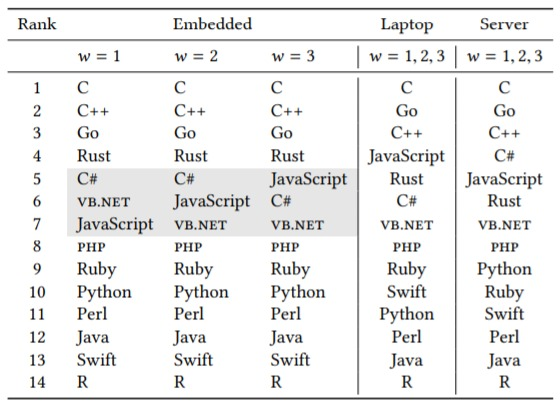
\includegraphics{figures/EDPranking.jpeg}
\caption{Programming Languages Average Weighted EDP Ranking, retrieved
from {[}\protect\hyperlink{ref-GKLS2018}{71}{]}}
\end{figure}

The above two papers are examples of research that suggest that the
current state of practice, developing applications in Java only, is not
in line with the current state of the art on energy efficiency. In spite
of these research papers, developers are still working mostly with Java.
One possible explanation is that Java is simply compatible with almost
every system due to the Java Virtual Machine (JVM). We suggest that
further research should investigate why developers are sticking to Java.
For example, looking at available libraries, coding difficulty and
available tools and knowledge might have a significant impact on this
choice.

\subsection{Answering SQ2}\label{answering-sq2}

In the previous sections, we have seen examples of the state of the art,
as well as development methods that could lead to improvements in energy
consumption. However, this knowledge only holds value when the community
can get developers willing to use these. There have been a number of
studies that look into what is actually happening.

One example is the paper by Moura et al.
{[}\protect\hyperlink{ref-MPEC2015}{135}{]}. In this paper, a study is
conducted by looking at a large number of energy-aware commits with
GitHub as the primary data source. This analysis has yielded a list of
approaches that are being used by developers in practice. These include:
frequency and voltage scaling, using power efficient libraries and more.
The study notes that the vast majority of the commits focus on the lower
levels of the software stack. Furthermore, only 16.2\% of the commits
were related to using more efficient libraries or data structures. There
are also a number of software qualities that have been shown to take
precedence of the energy consumption. These include correctness,
responsiveness, and performance. Another point which the research
addressed is whether software developers were certain of their energy
saving commits. The paper suggests that there are definitely cases where
developers are not certain about their energy saving change. This might
be caused by the fact that there are few user-friendly tools available
for aiding developers in making energy-aware decisions. One example of
such a tool that attempts to assist the developer in making energy
friendly decisions is jStanley
{[}\protect\hyperlink{ref-PSCS2018}{144}{]}. However, both the paper
itself and our own replication of that study indicate that this work is
not anywhere close to ideal. It only concerns the static analysis of the
code and is very limited in usability. This prevents such tools of being
used in practice. Additionally, there is the problem of how to actually
measure the energy being consumed. A number of papers explain how hard
this task actually is. Moura et al.
{[}\protect\hyperlink{ref-MPEC2015}{135}{]} also allude to the fact that
developers that do use third-party energy-management tools often lack
trust in the accuracy of the tools that they are using. The measuring of
energy-consumption is not actually as straightforward as one may think.
In a number of papers, it is explained how hardware-based solutions are
accurate but require expensive components. This is a serious issue,
especially in the field of mobile software development. On the other
hand, software-based solutions are cheaper but less accurate. Now there
is work being done on creating more accurate software solutions
{[}\protect\hyperlink{ref-NPPPZL2017}{57}{]}. Early work shows promising
results in combining the best of both worlds in order to obtain improved
results.

\section{RQ3: Future research}\label{rq3-future-research-1}

In this section, we will take a look at the suggested future research
directions that have been mentioned in the papers used in this survey.
We attempt to extract some general trends from the future research
suggestions that are included. A similarity between almost all of the
papers discussed in this section is that they agree the research field
is still not very mature. The conclusions of the majority of papers are
that more research is required. However, in this survey, we found that
the consensus is that it is hard to make strong claims, mainly due to
having doubts about both the measurement methods as well as the research
methodologies.

One of the fields of research we looked at in the previous sections was
the relation between programming languages and energy consumption.
Multiple papers suggest that the programming language used for
implementation has an influence on the energy consumption and
performance {[}\protect\hyperlink{ref-GKLS2018}{71},
\protect\hyperlink{ref-OOC2017}{139}{]}. These papers, however, do not
look into the influence of specific features of the programming
languages on energy consumption and performance. Or rather the specific
characteristics of a programming language that cause the differences, as
described in the paper by Georgiou et al.
{[}\protect\hyperlink{ref-GKLS2018}{71}{]}

In the investigations of this report, we came across a number of tools
which can be used to aid developers in their management of the energy
consumption of applications. However, to our knowledge, there are no
studies reporting on the actual use of such tools. For future research,
we suggest investigating the number of developers actually using such
tools. Furthermore, it is important which features should be included in
tools for optimal use. For example, we replicated the paper that
introduces jStanley, a tool which can be used for energy and performance
optimization {[}\protect\hyperlink{ref-PSCS2018}{144}{]}. We faced the
issue that this tool cannot implement the suggested improvements in an
easy and efficient way. For example, we took the AssertJ open source
project from GitHub and there were more than 300 energy saving
suggestions. A user has to click on every suggestion to actually
implement the improvement which is tedious work. Similarly, a lot of the
papers reporting on tools that could be used in practice, are currently
being tested with benchmarks. However, it is always the question whether
these benchmarks are representative enough of the real world to hold
actual merit. Additionally, the outcomes of the papers introducing these
tools are not comparable. Testing all these tools on the same project
would give better insights into what tools are actually useful for the
developers to use in terms of gaining as much energy efficiency as
possible.

Even though, to our knowledge, there have not been any studies into
whether the tools described in the research are actually been used in
practice, there have been some studies into energy-saving practices on
GitHub. For instance, studies into the commit messages
{[}\protect\hyperlink{ref-BLXWT2016}{14},
\protect\hyperlink{ref-MPEC2015}{135}{]} have shed some light into the
state of practice. These studies looked into the commit messages
containing keywords related to energy consumption and classified the
corresponding code. The future research directions that are indicated by
such papers is that it will be important to verify that the
energy-saving commits actually have an impact on the overall performance
of the software. That is both in terms of energy-consumption as well as
metrics for the performance related to usability. Similarly, another
direction is verifying that the energy-saving techniques are consistent
across platforms.

Finally, it is to be noted that nearly all research is based on
open-source projects from GitHub repositories. Research on proprietary
and closed-source software could possibly lead to different results and
would, therefore, be interesting to conduct.

\section{Conclusion}\label{conclusion-2}

Having answered the research questions of this chapter in the sections
above, we can conclude that energy awareness with regard to developing
applications for mobile devices, and more specific Android, needs more
attention. A lot of research is done in the field, resulting in
guidelines and tools to help developers. But these guidelines are very
generic and also conclude that energy awareness is project specific. The
tools presented by papers hold claims to improvements, but for example
the tested tool jStanley is not as easy to use as claimed in the paper.
More research into the claims made in the papers describing these tools
is needed. In practice, it is observed that the main language for
creating Android apps (Java) is not the most energy efficient option.
Furthermore, developers often do not give enough priority to energy
saving options and when they do they are often unsure about the effects
of their changes.

\chapter{App Store Analytics}\label{app-store-analytics}

\section{Motivation}\label{motivation-6}

In 2008, the first app stores became available
{[}\protect\hyperlink{ref-appStoreLaunch}{7}{]}{[}\protect\hyperlink{ref-androidMarketLaunch}{145}{]}.
These marketplaces have grown rapidly in size since then with over 3.8
million apps in the Google Play store the first quarter of 2018
{[}\protect\hyperlink{ref-appNumber}{172}{]}. These app stores, together
with a large amount of user-generated data associated with them present
an unprecedented source of information regarding the ecosystems of
modern software platforms, such as Android and iOS. Software developers
and researchers use these valuable data to gain new insights about how
users use their apps, what they like, and what difficulties they
encounter. The same data can be also used by app store operators for the
detection of malicious or misbehaving apps, i.e., whose behavior does
not match their app store description. Since these app stores are
relatively new, the research field of App Store Analytics is still not
mature. However, because apps are used to a great extent nowadays, their
investigation plays a vital role in the field of Software Engineering.

In 2015, Martin, William, et al., published a survey on app store
analytics for software engineering
{[}\protect\hyperlink{ref-martin2015survey}{121}{]}. The paper divides
the field of App Store Analytics into seven categories: API Analysis,
Review Analytics, Security, Store Ecosystem, Size, and Effort
Prediction, Release Engineering, and Feature Analysis. Given that
relevant literature on the field of App Store Analytics has been already
gathered and analyzed, it makes sense for us to use this chapter to go a
step further. We delve deeper into the subfield of Review Analytics. We
start with the literature proposed by Martin et al. in
{[}\protect\hyperlink{ref-martin2015survey}{121}{]} and extend it with
the relevant articles that were published after 2015. We then try to
answer the following research questions:

\begin{itemize}
\tightlist
\item
  \textbf{RQ1} What is the state of the art in Review Analytics?
  Specifically:

  \begin{itemize}
  \tightlist
  \item
    Which topics are being explored?
  \item
    Which research methods, tools, and datasets are being used?
  \item
    Which are the main research findings (aggregated)?
  \end{itemize}
\item
  \textbf{RQ2} What is the state of practice in Review Analytics?
  Specifically:

  \begin{itemize}
  \tightlist
  \item
    Which are the tools and the companies that create/employ them?
  \item
    Are there any case studies and which are the findings?
  \end{itemize}
\item
  \textbf{RQ3} Which are the challenges that the field is facing or will
  face?
\end{itemize}

\section{Research Protocol}\label{research-protocol-6}

In this section, we explain the process that we have followed to
systematically extract the appropriate facts from the articles for our
literature survey. The search strategy section includes the queries that
were used, as well as the initial criteria that were taken into account
for the initial filtering of the articles. Article selection explains
how the relevance of the papers was assessed, and how the final
filtering was done. The last section describes the data extracted from
each article.

\subsection{Search Strategy}\label{search-strategy-2}

As stated in the motivation, the survey by Martin et al.
{[}\protect\hyperlink{ref-martin2015survey}{121}{]} gave us a starting
point. Instead of gathering everything related to App Store Analytics we
decided to focus on extending the work done by the authors and answering
the research questions specifically related to the subcategory of Review
Analytics. We retrieved and inspected all the papers of the Review
Analytics category that were mentioned in the aforementioned survey and
we identified specific keywords and topics for our survey.

After doing this, the following search queries were generated:

\begin{verbatim}
“app store analytics” 
“app store analytics” AND “mining” 
“app store analytics” AND “user reviews” 
“app store analytics” AND “reviews”, “app reviews”
\end{verbatim}

Google Scholar\footnote{\url{https://scholar.google.com/}}, ACM Digital
Library\footnote{\url{https://dl.acm.org/}}, and IEEE Xplore\footnote{\url{https://ieeexplore.ieee.org/}}
were used for the searching process with the queries mentioned above. In
order to build a database using only the relevant articles, the
following inclusion criteria were applied. In addition to the results
obtained by searching with the specific queries, the first page of the
``related articles'' link for the top cited articles was also inspected.

\begin{longtable}[]{@{}ll@{}}
\toprule
\begin{minipage}[b]{0.22\columnwidth}\raggedright\strut
Criteria\strut
\end{minipage} & \begin{minipage}[b]{0.18\columnwidth}\raggedright\strut
Value\strut
\end{minipage}\tabularnewline
\midrule
\endhead
\begin{minipage}[t]{0.22\columnwidth}\raggedright\strut
time frame\strut
\end{minipage} & \begin{minipage}[t]{0.18\columnwidth}\raggedright\strut
2015-present\strut
\end{minipage}\tabularnewline
\begin{minipage}[t]{0.22\columnwidth}\raggedright\strut
journals and conferences\strut
\end{minipage} & \begin{minipage}[t]{0.18\columnwidth}\raggedright\strut
TSE, EMSE, JSS, IST, ICSE, FSE, MSR, OSDI, MobileSoft\strut
\end{minipage}\tabularnewline
\begin{minipage}[t]{0.22\columnwidth}\raggedright\strut
keywords in title\strut
\end{minipage} & \begin{minipage}[t]{0.18\columnwidth}\raggedright\strut
user reviews OR app store reviews\strut
\end{minipage}\tabularnewline
\begin{minipage}[t]{0.22\columnwidth}\raggedright\strut
keywords in abstract\strut
\end{minipage} & \begin{minipage}[t]{0.18\columnwidth}\raggedright\strut
user reviews OR app store reviews\strut
\end{minipage}\tabularnewline
\bottomrule
\end{longtable}

After the selection of the relevant papers, we gathered metadata
associated with them, and we entered them into a database. That was the
input for the next step of the survey, article selection.

\subsection{Article selection}\label{article-selection}

Taking into account that the papers considered in this survey were
published from 2015 and on, it is not a surprise that most of them are
not highly cited yet. As a consequence, the selection of the filtered
articles does not take the number of citations into consideration. In
contrast, each member of the group was in charge of delving into the
one-third of the papers of our database and finding, for each study, its
\emph{relevance} with respect to Review Analytics and the proposed
research questions. Then, that score was peer-reviewed by the other two
authors of our survey to achieve a consensus.

For the \emph{relevance} score, we considered how much the paper used
terms related to the analysis of user reviews. Next, we present three
examples: 1) a highly relevant paper score=10), 2) a somewhat relevant
paper (score=5) and 3) a non-relevant paper (score=0).

\textbf{What would users change in my app? Summarizing app reviews for
recommending software changes
{[}\protect\hyperlink{ref-di2016would}{58}{]}} - Relevance score: 10 -
Remarks: the authors applied classification and summarization techniques
on app reviews to reduce the effort required to analyze user feedback.
As it can be seen, the paper was focused on using the reviews to improve
the development process.

\textbf{Fault in your stars: an analysis of Android app reviews
{[}\protect\hyperlink{ref-aralikatte2018fault}{8}{]}} - Relevance score:
5 - Remarks: the authors analyzed the problem of the potential mismatch
between the reviews and the star ratings that apps receive. Although the
paper is related to app reviews, it is not its primary focus.

\textbf{Why are Android apps removed from Google Play? A large-scale
empirical study {[}\protect\hyperlink{ref-wang2018android}{187}{]}} -
Relevance score: 0 - Remarks: in this case, the paper did not have to do
with app reviews even though the title suggested that.

In the end, only the articles that had a score of 5 or more were used
for the fact extraction and the subsequent investigation of the research
questions.

\subsection{Fact extraction}\label{fact-extraction}

As it was mentioned before, the articles were listed in a database in a
structured fashion. The data that was extracted has the following
fields:

\begin{verbatim}
id for indexing
title
year 
relevance score 
relevance description 
source 
category
authors Information
source (journal or conference)
complete reference
\end{verbatim}

Additionally, for each one of the articles, a systematic reading was
carried out in which bullet points that answered the following questions
were generated:

\begin{verbatim}
Paper type
Research questions of the paper
Contributions
Datasets: size and sampling methodologies
Techniques used for doing the analysis 
\end{verbatim}

\section{Answers}\label{answers-5}

\subsection{\texorpdfstring{\textbf{RQ1} What is the state of the art in
Review Analytics?
Specifically:}{RQ1 What is the state of the art in Review Analytics? Specifically:}}\label{rq1-what-is-the-state-of-the-art-in-review-analytics-specifically}

\begin{itemize}
\tightlist
\item
  Which topics are being explored?
\item
  Which research methods, tools, and datasets are being used?
\item
  Which are the main research findings (aggregated)?
\end{itemize}

To answer the questions at hand, we looked at the novel ideas and the
research that has been done in the field of Review Analytics. In their
survey, Martin et al.
{[}\protect\hyperlink{ref-martin2015survey}{121}{]} proposed
``Classification'', ``Content'', ``Requirements Engineering'',
``Sentiment'', ``Summarization'' and ``Surveys and Methodological
Aspects of App Store Analysis'' to categorize the existing literature.
After analyzing the subsequent work, we suggest new categories that
reflect the state of the art in Review Analytics. These are: ``Review
Manipulation'', ``Requirements Engineering'', ``Mapping user reviews to
the source code'', ``Privacy / App Permissions'', ``Responding to
reviews'', ``Comparing Apps and App Stores'' and ``Wearables''. In the
following sections, we describe each one of these categories using the
new papers that we have found.

\textbf{Review Manipulation}

Recently, significant attention has been paid on how the reviews and
ratings can be used to influence the number of downloads of a particular
app in an App Store. The paper by Li et al.
{[}\protect\hyperlink{ref-i2017crowdsourced}{112}{]} analyzed the use of
crowdsourcing platforms such as Microworkers\footnote{\url{https://www.microworkers.com/}}
to manipulate the ratings. The authors merged data from two different
sources, an App Store and a crowdsourcing site, to identify manipulated
reviews.

Chen at al. {[}\protect\hyperlink{ref-chen2017toward}{41}{]} proposed an
approach to identify attackers of collusive promotion groups in an app
store. They use ranking changes and measurements of pairwise similarity
to form targeted app clusters (TAC) that they later use to pinpoint
attackers. A different approach to the same problem was proposed in
{[}\protect\hyperlink{ref-xie2016you}{191}{]}. In that paper, Xie et al.
identified manipulated app ratings based on the so-called attack
signatures. They presented a graph-based algorithm for achieving this
purpose in linear time.

These papers also show that the percentage of apps that manipulate their
reviews in the app stores is small --- less than 1 \% of the apps found
to be suspicious {[}\protect\hyperlink{ref-xie2016you}{191}{]}.
Regarding the datasets used in this category, the work done by Li et al.
{[}\protect\hyperlink{ref-i2017crowdsourced}{112}{]} used a smaller
amount of app store data, but they merged it with data from an external
crowdsourcing site. In the case of the other two previously presented
papers, they can be we can say that the authors have used a small number
of considered apps (compared to the total number of apps in the main
marketplaces), but the amount of the analyzed reviews was significant.
That makes sense, considering that the main purpose of both studies was
to examine app reviews.

\textbf{Requirements Engineering}

Users use reviews as a way to express their attitude (positive and
negative) towards an app. The information value of individual reviews is
usually low, but as a whole, they can be mined and provide useful
insights for the improvement and advancement of the apps. The survey by
Martin et al. {[}\protect\hyperlink{ref-martin2015survey}{121}{]}
described summarization, classification, and requirements engineering as
categories of the subfield of Review Analytics. These areas are
converging and in recent work (after 2015) summarization and
classification, among other techniques, are being used to complement the
development, maintenance, and evolution of the apps.

In 2016, Di Sorbo et al. introduced SURF
{[}\protect\hyperlink{ref-di2016would}{58}{]}, an approach to condense a
large number of reviews and extracting useful information from them. In
a subsequent paper Panichella et al.
{[}\protect\hyperlink{ref-panichella2016ardoc}{143}{]} presented
techniques for classifying useful feedback in the context of app
maintenance and evolution. In their work, the authors made use of
machine learning supervised methods in conjunction with natural language
processing (NLP), sentiment analysis (SA), and text analysis (TA)
techniques. Unsupervised methods for review clustering were explored in
a paper by Anchiêta et al.
{[}\protect\hyperlink{ref-anchieta2017}{6}{]}. The authors introduced a
technique to categorize reviews in order to generate a summary of bugs
and features of apps. Taking into account the high dimensionality of the
datasets that are used for review mining, Jha et al.
{[}\protect\hyperlink{ref-jha2017mining}{90}{]} proposed a semantic
approach for app review classification. By using semantic role labeling,
the authors could make the classification process more efficient. Gao et
al. presented IDEA {[}\protect\hyperlink{ref-gao2018online}{69}{]}; a
framework for identifying emerging app issues based on an online review
analysis. IDEA uses information from different time slices (versions)
for the identification of the issues, and the changelogs of the studied
apps as the ground truth for the validation of their approach. It is the
only paper in the reviewed literature that presents a case study (of
deployment in Tencent) as an example of the viability of IDEA.

Most of the datasets used in the papers we present in this section
analyze a small number of apps and a substantial amount of reviews. Di
Sorbo et al. {[}\protect\hyperlink{ref-di2016would}{58}{]} used 17 apps
and 3,439 reviews. Anchiêta et al.
{[}\protect\hyperlink{ref-anchieta2017}{6}{]} gathered more than 50,000
reviews from 3 apps, but after a preprocessing step, the dataset was
reduced to 924 records. Jha et al.
{[}\protect\hyperlink{ref-jha2017mining}{90}{]} used a structured
sampling procedure to mix reviews from different datasets. The final
size came to 2917 reviews. Finally, Gao et al.
{[}\protect\hyperlink{ref-gao2018online}{69}{]} used reviews from 6 apps
(2 from the App Store and 4 from Google Play), and the final dataset
contained 164,026 reviews. This study used one of the largest numbers of
reviews that have been ever studied.

\textbf{Mapping user reviews to source code}

Another research direction that has become active over the past years is
the combination of the mining results of app reviews with the source
code, to directly provide developers with valuable and actionable
information for the improvement of their products.

Palomba et al.
{[}\protect\hyperlink{ref-palomba2017recommending}{141}{]} presented a
new approach called ChangeAdvisor. It extracts useful feedback from
reviews and recommends changes to developers for specific code
artifacts. In the paper, metric distances such as the Dice coefficient
are used in order to map a specific subset of reviews to a particular
section in the source code. Complementary work was presented in
{[}\protect\hyperlink{ref-palomba2018crowdsourcing}{140}{]}. In this
study, Palomba et al. investigated the extent to which app developers
take app reviews into account. To achieve this, they introduced CRISTAL.
It pairs informative reviews with source code changes and monitors the
extent to which developers accommodate crowd requests from the reviews.

Linting mechanisms and their effectivity have been also studied. Wei et
al. {[}\protect\hyperlink{ref-wei2017oasis}{189}{]} proposed a method,
OASIS, for prioritizing the Android Lint warnings. It uses NLP
techniques (tokenization, word removing, word stemming, and TF-IDF
distance) to find links between user reviews and Lint warnings.
According to the paper, this is relevant given that one of the problems
of linters is the large number of false alarms they provide.

Regarding the datasets that were used for validation here, even though
the analyzed papers use a limited number of apps (except for
{[}\protect\hyperlink{ref-palomba2018crowdsourcing}{140}{]} that used
100), as stated in the previous section, they use numerous reviews (more
than 20,000). Additionally, as the aim of the works in this section
directly involve the developers, they have attempted to complete the
quantitatively apps-reviews-based experiments with qualitative ones.

\textbf{Privacy / app permissions}

Permission approaches used by mobile devices' software platforms have
been changed. Android Marshmallow the Android operating system uses a
run-time permission-based security system. Also, Apple's iOS also uses
run-time permissions on top of a set of permissions enabled by default.
Scoccia et al. did a large-scale empirical study on these new system
challenges by inspecting 4.3 million user reviews from 5,572 Google Play
store apps {[}\protect\hyperlink{ref-scoccia2018investigation}{165}{]}.
Using different techniques they extracted 3,574 user reviews that relate
to system permissions. They found that users like the minimal
permissions as most apps only ask for permissions they strictly need.
Some of the negative user concerns were apps asking for too many
permissions or asking for permissions at bad timing.

\textbf{Responding to reviews}

Developers can respond to reviews in the Google Play store from 2013.
Also, Apple introduced the same feature in 2017. In a previous work,
McIlroy {[}\protect\hyperlink{ref-mcilroy2014empirical}{125}{]} studied
whether responding to user reviews has a positive effect on the rating
users give. Building on previous work, McIlroy et al. studied how likely
it is for users to change their rating for an app when a developer
responds to their review
{[}\protect\hyperlink{ref-mcilroy2017worth}{126}{]}. They found that
users change their rating, with probability 38.7 percent, when a
developer responds to their review, and with a median increase of 20
percent in rating for an app.

Hassan et al. {[}\protect\hyperlink{ref-hassan2018studying}{81}{]} used
2,328 top free apps from the Google Play store to study whether users
are more likely to update their reviews if a developer responds to
these. They extracted 126,686 dialogues between developers and users and
concluded that responding to a review increases the chances of users
updating their given rating for an app by up to six times compared to
not responding. They also studied the characteristics, likelihood, and
the incentives of user-developer dialogues in app stores.

\textbf{Comparing Apps and App stores}

Papers that compare apps or app stores are discussed in this section. Li
et al. mined user reviews from Google Play to find comparisons between
apps {[}\protect\hyperlink{ref-li2017mining}{113}{]}. They set out to
identify comparative reviews to extract differences between apps on
different topics. For example, a user says in a review that this app is
not as good regarding power consumption as another app. Li et al.
created a method that with sufficient accuracy extracts these opinions
and provides comparisons between apps.

Ali et al. did a comparative study on cross-platform apps. They took a
sample of 80.000 app-pairs to quantitatively compare the same apps
across different platforms and identify the differences among software
platforms {[}\protect\hyperlink{ref-ali2017same}{5}{]}.\\
In a related study, Hu et al. compared app-pairs that are created using
hybrid development tools such as PhoneGap
{[}\protect\hyperlink{ref-hu2018studying}{86}{]}. With this approach,
they found that in 33 of the 68 app-pairs the star rating was not
consistent across platforms.

\textbf{Wearables}

User reviews can be also used for understanding user complaints. Mujahid
et al. did this in a case study on Android Wear
{[}\protect\hyperlink{ref-mujahid2017examining}{136}{]}. More
specifically, they sampled 589 reviews from 6 Android wearable apps and
found that 15 unique complaint types could be extracted from the sample.
The sample was created from mining the reviews of 4,722 wearable apps
and selecting the apps that had more than 100 reviews with a rating of
one or two stars. After manually assigning categories to the reviews in
the sample, they concluded that the most frequent complaints in this
relatively small sample were complaints related to cost, functional
errors, and a lack of functionality.

\subsection{\texorpdfstring{\textbf{RQ2} What is the state of practice
in Review Analytics?
Specifically:}{RQ2 What is the state of practice in Review Analytics? Specifically:}}\label{rq2-what-is-the-state-of-practice-in-review-analytics-specifically}

\begin{itemize}
\tightlist
\item
  Which are the tools and the companies that create/employ them?
\item
  Case studies and the findings.
\end{itemize}

A large amount of work has been published in the field of app store
analytics (the survey by Martin et al. was done on over 250 papers, and
our study additionally analyzed 80 papers), only a few of them were case
studies. After applying the article selection criteria, we were left
with 30 papers from which only two conducted a case study. The first
case study of this selection, done by Mujahid et al.
{[}\protect\hyperlink{ref-mujahid2017examining}{136}{]}, examines issues
that bother the users of Android Wear. The second one, done by Gao et
al. {[}\protect\hyperlink{ref-gao2018online}{69}{]}, reports on the
performance of their review analytics tool which was deployed at
Tencent. This creates a large gap between the number of proposed
solutions by the researchers and the number of studies done on the
solutions that had been deployed in practice.

\subsubsection{State of the app stores}\label{state-of-the-app-stores}

We were not able to find any academic publication on the solutions used
by the actual app stores (Google Play and App Store), but we have found
that both app stores automatically detect fake reviews,\footnote{\url{https://www.macrumors.com/2016/10/10/apple-dash-developer-fraudulent-reviews/}}\footnote{\url{https://android-developers.googleblog.com/2016/11/keeping-it-real-improving-reviews-and-ratings-in-google-play.html}}.
In 2016 Google deployed their review analytics solution, called Review
Highlights\footnote{\url{https://android-developers.googleblog.com/2016/02/new-tools-for-ratings-reviews-on-google.html}},
into production for both developers and customers, but at the time of
writing this survey (October 2018), the Review Highlights no longer show
up in the public facing part of Google Play Store and are only
accessible in the developer's console\footnote{\url{https://support.google.com/googleplay/android-developer/answer/138230?hl=en}}.

\subsubsection{State of the third-party
tools}\label{state-of-the-third-party-tools}

Many third-party services focus on app store analysis. They usually
focus on showing aggregated statistics from the app stores and some of
them also analyze user reviews. Tools such as AppBot\footnote{\url{https://appbot.co/}}
or TheTool\footnote{\url{https://thetool.io/}} perform sentiment
analysis on the reviews and show it as an additional metric next to the
star rating. AppBot also categorizes reviews based on the keywords
inside them. It may seem like a low-tech approach, but it makes it easy
for the users to reason about why a certain review is assigned to a
specific category. We were not able to find any third-party tools that
would use any of the advanced Machine Learning algorithms from the
papers we analyzed. This finding combined with Google hiding their
Review Highlights may show that most of the algorithms proposed by the
researchers do not generalize very well in the real-world application
and are hard to comprehend by regular users.

To this day there are, to the best of our knowledge, no tools that
compare apps and app stores using user reviews. Some tools analyze apps
and app performance, but there are no tools that do comparisons.

\subsection{\texorpdfstring{\textbf{RQ3} Which are the challenges that
the field is facing or will
face?}{RQ3 Which are the challenges that the field is facing or will face?}}\label{rq3-which-are-the-challenges-that-the-field-is-facing-or-will-face}

In this section, we present challenges and future research directions
for the field of Review Analytics and the subcategories that were
identified in previous sections.

A significant aspect of the research process is the validation of the
proposed tools and frameworks and the assessment of how generalizable
they are. To accomplish this, it is necessary for researchers to have
large datasets of reviews and more representative and sound samples.
Machine learning has seen a steady increase in popularity, however, it
has not been used a lot in the field of Review Analytics. Also, most of
the studies rely on correlation relationships to validate the
effectiveness of their approaches. There is a need to apply causation
techniques so confounding factors can be ruled out.

There is a difficulty in trasforming research into actual tools that are
used in a real-world setting. Of all the works that were considered
here, only Gao et al. presented a case study
{[}\protect\hyperlink{ref-gao2018online}{69}{]}, and most of the tools
from other papers are either unavailable or not actively used.

\emph{Review Manipulation:} It is important to combine multiple sources
of data to identify suspicious apps. Not just from app stores alone, but
also from crowdsourcing sites and even from social networks. Also, the
sample should be carefully selected, given that the number of suspicious
apps is not significant (around 1\% of all apps), taking into account
the size of the app stores.

\emph{Requirements Engineering:} More case studies are needed in order
to validate how useful the extracted requirements are in the context of
software development. Also, as machine learning is starting to be
heavily used, models that are tailored to the review data are expected
to be created. The large amounts of noise that is present in the reviews
is still a challenge that needs careful studying of the preprocessing
steps that are used while assembling the datasets.

\emph{Mapping user reviews to source code:} There is a need for
developers to improve their programs by combining reviews with source
code datasets. A likely future trend is the analysis of update-level
changes. Regarding this, there is still a need to obtain
update-categorized reviews as this is still a challenge for the current
review-retrieving approaches.

\emph{Privacy/app permissions:} Quantifying and understanding the
effects of run-time permission requests on the user experience is still
an open research area which can help developers to increase the quality
of their apps. One of the directions for further research regarding
permissions is the idea of giving permissions to specific app
functionalities instead of giving permissions to the app as a whole.
That could lead to better user-understanding why an app needs certain
permission and could reduce the number of permissions an app needs.
Another possible future direction is researching and creating tools that
help developers put permission requests in the right place to avoid bugs
related to permissions and permission requests.

\emph{Responding to reviews:} There is a need for an in-depth study of
how developers and users are using the review mechanism to find out how
this mechanism can be improved. Right now developers respond to almost
500 user reviews per day using the Google Play API\footnote{\url{https://developers.google.com/android-publisher/reply-to-reviews}}.
It could be worth investigating whether a limit of 500 responses is
sufficient to ban useless responses from the store such as thanking
every user.

\emph{Comparing Apps and App stores:} One of the open challenges is
including indirect relationships in the comparisons as only direct
relationships were used in work by Li et al.
{[}\protect\hyperlink{ref-li2017mining}{113}{]}. Next, to this, it has
been noted that apps that have been developed using hybrid development
tools had relatively low ratings. Future studies should be done to
investigate the quality of hybrid apps and compare them with the quality
of native apps. Furthermore, to get more complete results, current
research approaches should focus on a market-scale analysis using a
large number of apps and reviews.

\chapter{Final Words}\label{final-words}

We have finished a nice book on Software Analytics.

\appendix


\section{Appendix to Chapter 7 (Code
Review)}\label{appendix-to-chapter-7-code-review}

\subsection{Extracted data}\label{extracted-data}

This section contains data extracted from all resources included in the
survey, according to the \emph{Data collection} section of the review
protocol. Note that if some data could not be collected, it is
explicitly stated.

The resources are listed in alphabetical order of first author name, and
then by year published.

\subsubsection{Expectations, outcomes, and challenges of modern code
review}\label{expectations-outcomes-and-challenges-of-modern-code-review}

Reference: {[}\protect\hyperlink{ref-bacchelli2013expectations}{11}{]}

\textbf{Summary}

This paper describes research about the goals and actual effects of code
reviews. Interviews and experiments have been done with people in the
programming field.

One of the main conclusions is that the main effect of doing code
reviews is that everyone involved understands the code better. This is
opposed to what the goal of code reviews generally is: discovering
errors.

For answering \textbf{RQ1}:

\begin{itemize}
\tightlist
\item
  \emph{Sub-topic}: in practice; tools
\item
  \emph{Research method}: empirical; qualitative
\item
  \emph{Tools}: N/A
\item
  \emph{Datasets}: Data collected from interviews, surveys and code
  reviews
\end{itemize}

\textbf{Research questions and answers}:

\begin{itemize}
\tightlist
\item
  \emph{What are the motivations and expectations for modern code
  review? Do they change from managers to developers and testers?} The
  top motivation for code reviews is finding defects, closely followed
  by code improvement. There does not seem to be a large difference
  between managers, developers and testers.
\item
  \emph{What are the actual outcomes of modern code review? Do they
  match the expectations?} Code improvements are the most seen outcomes
  of code review, followed by code understanding and social
  communication. The outcomes do not match the expectations well. For
  example, only 14\% of researched review comments was about code
  defects, while about 44\% chose finding defects as the main motivation
  for doing code review.
\item
  \emph{What are the main challenges experienced when performing modern
  code reviews relative to the expectations and outcomes?} The main
  challenges is by far understanding the code under review. This occurs
  for example when code has to be reviewed that is not in the same
  system as a developers works on daily.
\end{itemize}

For answering \textbf{RQ2}:

\begin{itemize}
\tightlist
\item
  \emph{Tools used}: CodeFlow, a reviewing tool. It is not publicly
  available.
\item
  \emph{Company/organization}: Microsoft
\item
  \emph{Evaluation}: At the time of this paper, it still focusses mainly
  on fixing errors, and not on the more often ocurring results of doing
  code review.
\end{itemize}

For answering \textbf{RQ3}:

\textbf{Future research challenges}:

\begin{itemize}
\tightlist
\item
  Research on automating code review tasks. This mainly concerns
  low-level tasks, like checking boundary conditions or catching common
  mistakes.
\item
  Research on code comprehension during code review. According to the
  authors research has been done on this with new developers in mind,
  but it would also be applicable to code reviews. The authors note that
  IDEs often include tools for code comprehension, but code review tools
  do not.
\item
  Research on awareness and learning during code review. Those two
  aspects were cited as motivations for code review by developers.
  Future research could research these aspects more explicitly.
\end{itemize}

\subsubsection{A Faceted Classification Scheme for Change-Based
Industrial Code Review
Processes}\label{a-faceted-classification-scheme-for-change-based-industrial-code-review-processes}

Reference: {[}\protect\hyperlink{ref-baum2016faceted}{16}{]}

\textbf{Summary} The broad research questions answered in this article
are: How is code review performed in industry today? Which commonalities
and variations exist between code review processes of different teams
and companies? The article describes a classification scheme for
change-based code review processes in industry. This scheme is based on
descriptions of the code review processes of eleven companies, obtained
from interviews with software engineering professionals that were
performed during a Grounded Theory study.

\subsubsection{The Choice of Code Review Process: A Survey on the State
of the
Practice}\label{the-choice-of-code-review-process-a-survey-on-the-state-of-the-practice}

Reference: {[}\protect\hyperlink{ref-baum2017choice}{15}{]}

\textbf{Summary} This paper, published in 2017, is trying to answer 3
RQs. Firstly, how prevalent is change-based review in the industry?
Secondly, does the chance that code review remains in use increase if
code review is embedded into the process (and its supporting tools) so
that it does not require a conscious decision to do a review? Thirdly,
are the intended and acceptable levels of review effects a mediator in
determining the code review process?

\subsubsection{The influence of non-technical factors on code
review}\label{the-influence-of-non-technical-factors-on-code-review}

Reference: {[}\protect\hyperlink{ref-baysal2013influence}{19}{]}

\textbf{Summary} This paper focus on the influence of several
non-technical factors on code review response time and outcome. An
empirical study of code review process for WebKit, a large open source
project was described to see the influence. Specifically, the authors
replicated some previously studied factors and extended several more
factors that had not beed explored.

For answering \textbf{RQ1}:

\begin{itemize}
\tightlist
\item
  \emph{Sub-topic}: open-source, impact
\item
  \emph{Research method}: empirical study
\item
  \emph{Tools}: WebKit
\item
  \emph{Datasets}: WebKit code review data extracted from Bugzilla.
\end{itemize}

\textbf{Research questions and answers}:

\begin{itemize}
\item
  \emph{What factors can influence how long it takes for a patch to be
  reviewed?} The organizational and personal factors influence review
  timeliness. Some factors that influenced the time required to review a
  patch, such as the size of the patch itself or the part of the code
  base being modified, are unsurprising and are likely related to the
  technical complexity of a given change. The most influential factors
  of the code review process on review time are the organization a patch
  writer is affiliated with and their level of participation within the
  project.
\item
  \emph{What factors influence the outcome of the review process?} The
  organizational and personal factors influence the likelihood of a
  patch being accepted. The most influential factors of the code review
  process on patch acceptance are the organization a patch writer is
  affiliated with and their level of participation within the project.
\end{itemize}

For answering \textbf{RQ3}:

\textbf{Future research challenges}:

\begin{itemize}
\tightlist
\item
  Research on studying how best to interpret empirical software
  engineering research within the context of contextual factors.
  Understanding the reasons behind observable developer behaviour
  requires an understanding of the contexts, processes, organizational
  and individual factors that can influence code review and its outcome.
\end{itemize}

\textbf{Notes}:

This paper has an extended version
{[}\protect\hyperlink{ref-baysal2016investigating}{18}{]}.

\subsubsection{Investigating technical and non-technical factors
influencing modern code
review}\label{investigating-technical-and-non-technical-factors-influencing-modern-code-review}

Reference: {[}\protect\hyperlink{ref-baysal2016investigating}{18}{]}

\textbf{Summary}:

This article primirarily discusses some non-technical factors that
influence the code review process. This are factors like review
experience, amount of contributions to a project and company
affiliation.

It is found that the most important factors influencing the code review
process, in terms of both review time and patch acceptance, are the
organization affiliation of the patch writer and the amount of
participation of the patch writer in the project.

For answering \textbf{RQ1}:

\begin{itemize}
\tightlist
\item
  \emph{Sub-topic}: non-technical
\item
  \emph{Research method}: empirical; quantitative
\item
  \emph{Tools}: Custom
\item
  \emph{Datasets}: WebKit reviews, Google Blink reviews
\end{itemize}

\textbf{Research questions and answers}:

\begin{itemize}
\item
  \emph{What factors can influence how long it takes for a patch to be
  reviewed?} ``Based on the results of two empirical studies, we found
  that both technical (patch size and component) , as well as
  non-technical (organization, patch writer experience, and reviewer
  activity) factors affect review timeliness when studying the effect of
  individual variables. While priority appears to influence review time
  for WebKit, we were not able to confirm this for Blink.''
\item
  \emph{What factors influence the outcome of the review process?} ``Our
  findings from both studies suggest that patch writer experience
  affects code review outcome. For the WebKit project, factors like
  priority, organization, and review queue also have an effect on the
  patch acceptance.''
\end{itemize}

For answering \textbf{RQ2}:

\begin{itemize}
\tightlist
\item
  \emph{Tools}: N/A
\item
  \emph{Company/Organization}: N/A
\item
  \emph{Evaluation}: N/A
\end{itemize}

\textbf{Notes}:

This paper has a shorter version
{[}\protect\hyperlink{ref-baysal2013influence}{19}{]}.

For answering \textbf{RQ3}:

\textbf{Future research challenges}:

Not stated

\subsubsection{Modern code reviews in open-source projects: Which
problems do they
fix?}\label{modern-code-reviews-in-open-source-projects-which-problems-do-they-fix}

Reference: {[}\protect\hyperlink{ref-beller2014modern}{21}{]}

\textbf{Summary} It has been researched what kinds of problems are
solved by doing code reviews. The conclusion is that 75\% are
improvements in evolvability of the code, and 25\% in functional
aspects.

It has also been researched which part of the review comments is
actually followed up by an action, and which part of the edits after a
review are actually caused by review comments.

For answering \textbf{RQ1}:

\begin{itemize}
\tightlist
\item
  \emph{Sub-topic}: impact,changes
\item
  \emph{Research method}: empirically explore; change classification
\item
  \emph{Tools}: R
\item
  \emph{Datasets}: documented history of ConQAT and GROMACS
\end{itemize}

\textbf{Research questions and answers}:

\begin{itemize}
\tightlist
\item
  \emph{Which types of changes occur in code under review?} 75\% of
  changes are related to the evolvability of the system, and only 25\%
  to its functionality.
\item
  \emph{What triggered the changes occurring in code under review?}
  78-90\% of the trigger are review comments and the remaining 10-22\%
  are `undocumented'.
\item
  \emph{What influences the number of changes in code under review?}
  Code churn, number of changed files and task type are the most
  important factors influencing the number of changes.
\end{itemize}

\subsubsection{Lessons learned from building and deploying a code review
analytics
platform}\label{lessons-learned-from-building-and-deploying-a-code-review-analytics-platform}

Reference: {[}\protect\hyperlink{ref-bird2015lessons}{29}{]}

\textbf{Summary}:

A code review data analyzation platform developed and used by Microsoft
is discussed. It is mainly presented what users of the system think of
it and how its use influences development teams. One of the conclusions
is that in general, the platform has a positive influence on development
teams and their products.

For answering \textbf{RQ2}:

\begin{itemize}
\tightlist
\item
  \emph{Tools used:} CodeFlow, CodeFlow Analytics
\item
  \emph{Company/organization using the tool:} Microsoft
\item
  \emph{Evaluation of the tool:} CodeFlow has already had a positive
  implace on development teams because of its simplicity, low barrier
  for feedback and flexible support of Microsoft's disparate engineering
  systems. But some challenges such as dealing with branches and linking
  reviews to commits need to improve.
\end{itemize}

As for CodeFlow Analytics: the tool is being used increasingly
throughout Microsoft, with different teams using the tool for different
purposes. It is for example effectively used to create dashboards with
code review evaluation information, or for examining past reviews in
detail. However, some parts of the tool still need to improve in terms
of user-friendliness, for example because some functionality is
difficult to find.

For answering \textbf{RQ3}:

\textbf{Future research challenges}:

\begin{itemize}
\tightlist
\item
  Research on an automatic way to classify and assess the usefulness of
  comments. This was specifically requested by an interviewees's and is
  still an open challenge regarding CodeFlow.
\item
  Research on many aspects of code review based on data from CodeFlow
  Analytics or other similar tools.
\item
  Research on methods to automatically recommend reviewers for changes
  in the system.
\end{itemize}

\subsubsection{Software Reviews: The State of the
Practice}\label{software-reviews-the-state-of-the-practice}

Reference: {[}\protect\hyperlink{ref-ciolkowski2003software}{42}{]}

\textbf{Summary} To investigate how industry carries out software
reviews and in what forms, this paper conducted a two-part survey in
2002, the first part based on a national initiative in Germany and the
second involving companies worldwide. Additionally, this paper also
include some fundamental concepts of code review, such as
functionalities of code review.

\subsubsection{Code reviews do not find bugs: how the current code
review best practice slows us
down}\label{code-reviews-do-not-find-bugs-how-the-current-code-review-best-practice-slows-us-down}

Reference: {[}\protect\hyperlink{ref-czerwonka2015code}{52}{]}

\textbf{Summary} As code review has many uses and benefits, the authors
hope to find out whether the current code review methods are
sufficiently efficient. They also research whether other methods may be
more efficient. With experience gained at Microsoft and with support of
data, the authors posit (1) that code reviews often do not find
functionality issues that should block a code submission; (2) that
effective code reviews should be performed by people with a specific set
of skills; and (3) that the social aspect of code reviews cannot be
ignored.

For answering \textbf{RQ1}:

\begin{itemize}
\tightlist
\item
  \emph{Sub-topic}: impact
\item
  \emph{Research method}: empirical
\item
  \emph{Tools}: not mentioned
\item
  \emph{Datasets}: data collected from engineering systems
\end{itemize}

\textbf{Research questions and answers}:

\begin{itemize}
\tightlist
\item
  \emph{In what situations, do code reviews provide more value than
  others?} Unlike inspections, code reviews do not require participants
  to be in the same place nor do they happen at a fixed, prearranged
  time. Aligning with a distributed nature of many projects, code
  reviews are asynchronous and frequently supporting geographically
  distributed reviewers.
\item
  \emph{What is the value of consistency of applying code reviews
  equally to all code changes?} Code review usefulness is negatively
  correlated with the size of a code review. With 20 or more changed
  files, the more files there are in a single review, the lower the
  overall rate of useful feedback.
\end{itemize}

For answering \textbf{RQ3}:

\textbf{Future research challenges}:

\begin{itemize}
\item
  Research on undocumented changes of code review because prior research
  has neglected.
\item
  Due to its costs, code reviewing practice is a topic deserving to be
  better understood, systematized and applied to software engineering
  workflow with more precision than the best practice currently
  prescribes.
\end{itemize}

\subsubsection{Design and code inspections to reduce errors in program
development}\label{design-and-code-inspections-to-reduce-errors-in-program-development}

Reference: {[}\protect\hyperlink{ref-fagan2002design}{66}{]}

\textbf{Summary} This paper describes a method to thoroughly check code
quality after each step of the development process, in a heavyweight
manner. It does not really concern agile development.

The authors state that these methods do not affect the developing
process negatively, and that they work well for improving software
quality.

\subsubsection{An exploratory study of the pull-based software
development
model}\label{an-exploratory-study-of-the-pull-based-software-development-model}

Reference: {[}\protect\hyperlink{ref-gousios2014exploratory}{74}{]}

\textbf{Summary} This article focuses on how much pull requests are
being used and how they are used, focusing on GitHub. For example, it is
concluded that pull-requests are not being used that much, that
pull-requests are being merged fast after they have been submitted, and
that a pull request not being merged is most of the time not caused by
technical errors in the pull-request.

For answering \textbf{RQ1}:

\begin{itemize}
\tightlist
\item
  \emph{Sub-topic}: open-source, in practice
\item
  \emph{Research method}: empirical; qualitative for finding out reasons
  for closing pull request, rest quantitative.
\item
  \emph{Tools}: Custom developed tools, available online
\item
  \emph{Datasets}: GHTorrent dataset, along with data collected by
  authors. The last is also available online
\end{itemize}

\textbf{Research questions and answers}:

\begin{itemize}
\tightlist
\item
  \emph{How popular is the pull based development model?} ``14\% of
  repositories are using pull requests on Github. Pull requests and
  shared repositories are equally used among projects. Pull request
  usage is increasing in absolute numbers, even though the proportion of
  repositories using pull requests has decreased slightly.''
\item
  \emph{What are the lifecycle characteristics of pull requests?} ``Most
  pull requests are less than 20 lines long and processed (merged or
  discarded) in less than 1 day. The discussion spans on average to 3
  comments, while code reviews affect the time to merge a pull request.
  Inclusion of test code does not affect the time or the decision to
  merge a pull request. Pull requests receive no special treatment,
  irrespective whether they come from contributors or the core team.''
\item
  \emph{What factors affect the decision and the time required to merge
  a pull request?} ``The decision to merge a pull request is mainly
  influenced by whether the pull request modifies recently modified
  code. The time to merge is influenced by the developer's previous
  track record, the size of the project and its test coverage and the
  project's openness to external contributions.''
\item
  \emph{Why are some pull requests not merged?} ``53\% of pull requests
  are rejected for reasons having to do with the distributed nature of
  pull based development. Only 13\% of the pull requests are rejected
  due to technical reasons.''
\end{itemize}

For answering \textbf{RQ2}:

\begin{itemize}
\tightlist
\item
  \emph{Tools used}: GitHub PR system
\item
  \emph{Company/organization}: Several open-source projects
\item
  \emph{Evaluation}: N/A
\end{itemize}

For answering \textbf{RQ3}:

\textbf{Future research challenges}:

\begin{itemize}
\tightlist
\item
  More research is needed on \emph{drive-by commits}, which the paper
  loosely defines as commits added to a repository through a PR by a
  user that has never contributed to the repository and hence does so
  for the first time. Often this new contributor also has created a fork
  for the sole purpose of creating this PR. More research is needed on
  accurately defining drive-by commits and on assessing their
  implications.
\item
  More research is needed on the effect of the democratization of the
  develoment process, which occurs for example through the use of pull
  requests. Democratization could for example lead to a substantially
  stronger commons ecosystem.
\item
  Validating the used models on data from different sources and on
  projects on different languages.
\item
  Research on the motives of developers to work in a highly transparent
  workspace.
\item
  Research on formation of teams and management hierarchies with respect
  to open-source projects.
\item
  Research on novel code review practices.
\item
  Research on ways to managing tasks in the pull-based development
  model.
\end{itemize}

\textbf{Challenges in practice}:

\begin{itemize}
\tightlist
\item
  Development of tools to help the core team of a project with
  prioritizing their work. The paper gives as an example a tool which
  would suggest whether a pull request can be merged or not, because
  this can be predicted with fairly high accuracy.
\item
  Development of tools that would suggest categories of improvement for
  pull request, for example by suggesting that more documentation needs
  to be added.
\end{itemize}

\subsubsection{The impact of code review coverage and code review
participation on software quality: A case study of the qt, vtk, and itk
projects}\label{the-impact-of-code-review-coverage-and-code-review-participation-on-software-quality-a-case-study-of-the-qt-vtk-and-itk-projects}

Reference: {[}\protect\hyperlink{ref-mcintosh2014impact}{129}{]}

\textbf{Summary} This paper focuses on the influence of doing
light-weight code reviews on software quality. In particular, the effect
of review coverage (the part of the code that has been reviewed) and
review participation (a measure for how much reviewers are involved in
the review process) are being assessed.

It turns out that both aspects improve software quality when they are
higher. Review participation is the most influential. According to the
authors there are other aspects, which they have not looked into, that
are of significant importance for the review process.

For answering \textbf{RQ1}:

\begin{itemize}
\tightlist
\item
  \emph{Sub-topic}: open-source, in practice, impact
\item
  \emph{Research method}: qualitative for finding out the impact of code
  review coverage and code review participation on software quality rest
  quantitative.
\item
  \emph{Tools}: N/A
\item
  \emph{Datasets}: Data extracted from Qt, VTK and ITK code review
  dataset and necessary metrics including version control metrics,
  coverage metrics and participation metrics.
\end{itemize}

\textbf{Research questions and answers}:

\begin{itemize}
\item
  \emph{Is there a relationship between code review coverage and
  post-release defects?} Although review coverage is negatively
  associated with software quality in our models, several defect-prone
  components have high coverage rates, suggesting that other properties
  of the code review process are at play.
\item
  \emph{Is there a relationship between code review participation and
  post-release defects?} Lack of participation in code review has a
  negative impact on software quality. Reviews without discussion are
  associated with higher post-release defect counts, suggesting that the
  amount of discussion generated during review should be considered when
  making integration decisions.
\end{itemize}

For answering \textbf{RQ2}:

\begin{itemize}
\tightlist
\item
  \emph{Tools}: Gerrit
\item
  \emph{Company/Organization}: N/A
\item
  \emph{Evaluation}: N/A
\end{itemize}

For answering \textbf{RQ3}:

\textbf{Future research challenges}:

\begin{itemize}
\tightlist
\item
  Research on other properties of modern code review such as code
  ownership. Inspired by this paper, other properties of modern code
  review can also be explored.
\end{itemize}

\textbf{Notes}:

There exists an extended and improved version of this paper
{[}\protect\hyperlink{ref-mcintosh2016empirical}{128}{]}. Only the
original version of the paper has been included in this survey.

\subsubsection{A Study of the Quality-Impacting Practices of Modern Code
Review at Sony
Mobile}\label{a-study-of-the-quality-impacting-practices-of-modern-code-review-at-sony-mobile}

Reference: {[}\protect\hyperlink{ref-shimagaki2016study}{168}{]}

\textbf{Summary} First the study by McIntosh et al.
{[}\protect\hyperlink{ref-mcintosh2016empirical}{128}{]} is replicated
in a proprietary setting at Sony Mobile. A qualitative study, including
interviews, is also done with the question ``Why are certain reviewing
practices associated with better software quality?''

The results from this study are the same as those from the replicated
study for RQ1, but not for RQ2. Also, what has been found has been
confirmed by the quanitative study has been supported by the qualitative
study.

For answering \textbf{RQ1}:

\begin{itemize}
\tightlist
\item
  \emph{Sub-topic}:
\item
  \emph{Research method}: replication: empirical, quantitative;
  qualitative
\item
  \emph{Tools}: N/A
\item
  \emph{Datasets}: Review data from Sony Mobile
\end{itemize}

\textbf{Research questions and answers}:

\begin{itemize}
\item
  \emph{Is there a relationship between code review coverage and
  post-release defects?} ``Although our review coverage model
  outperforms our baseline model, of the three studied review coverage
  metrics, only the proportion of In-House contributions contributes
  significantly to our model fits. Comparison with previous work.
  Similar to the prior work
  {[}\protect\hyperlink{ref-mcintosh2016empirical}{128}{]}, we find that
  Reviewed Commit and Reviewed Churn provide little explanatory power,
  suggesting that other reviewing factors are at play.''
\item
  \emph{Is there a relationship between code review participation and
  post-release defects?} ``Our review participation model also
  outperforms our baseline model. Of the studied review participation
  metrics, only the measure of accumulated effort to improve code
  changes (Patch Sd) and the rate of author self-verification (Self
  Verify) contribute significantly to our model fits. Comparison with
  previous work. Unlike the prior work
  {[}\protect\hyperlink{ref-mcintosh2016empirical}{128}{]}, code
  reviewing time and discussion length did not provide exploratory power
  to the Sony Mobile model''
\end{itemize}

For answering \textbf{RQ2}:

\begin{itemize}
\tightlist
\item
  \emph{Tools}: Gerrit
\item
  \emph{Company/Organization}: Sony Mobile
\item
  \emph{Evaluation}: N/A
\end{itemize}

For answering \textbf{RQ3}:

\textbf{Future research challenges}:

Not stated

\subsubsection{ReDA: A Web-based Visualization Tool for Analyzing Modern
Code Review
Dataset}\label{reda-a-web-based-visualization-tool-for-analyzing-modern-code-review-dataset}

Reference: {[}\protect\hyperlink{ref-thongtanunam2014reda}{181}{]}

\textbf{Summary}:

This paper intoduces \emph{ReDA}, a web-based visualization tool for
code review datasets. It processes data from Gerrit, presents statistics
about the data, visualizes it, and points the user towards possible
problems occurring during the review process. It was tested briefly on
some open-source projects.

For answering \textbf{RQ1}:

\begin{itemize}
\tightlist
\item
  \emph{Sub-topic}: visualization; tools
\item
  \emph{Research method}: qualitative; empirical
\item
  \emph{Tools}: ReDA
\item
  \emph{Datasets}: Android code review data
\end{itemize}

\textbf{Research questions and answers}:

N/A

For answering \textbf{RQ2}:

\begin{itemize}
\tightlist
\item
  \emph{Tools}: N/A
\item
  \emph{Company/Organization}: N/A
\item
  \emph{Evaluation}: N/A
\end{itemize}

For answering \textbf{RQ3}:

\textbf{Future research challenges}:

The authors aim to develop a live code review monitoring dashboard based
on ReDA. They also aim to create a more portable version of ReDA that is
also compatible with other tools supporting the MCR process.

\subsubsection{Who should review my code? A file location-based
code-reviewer recommendation approach for modern code
review}\label{who-should-review-my-code-a-file-location-based-code-reviewer-recommendation-approach-for-modern-code-review}

Reference: {[}\protect\hyperlink{ref-thongtanunam2015should}{180}{]}

\textbf{Summary}:

This paper presents (1) research on how often a reviewer cannot be found
for a code change and the influence of this on the time it takes to
process a code change, (2) a tool (\emph{RevFinder}) for automatically
suggesting reviewers based on files reviewed previously, and (3) an
empirical evaluation of that tool on four open-source projects.

Of the researched projects, up to 30\% of the code changes have problems
finding a reviewer. These reviews take on average 12 days longer. Also,
it is found that RevFinder works 3 to 4 times better than an existing
tool.

For answering \textbf{RQ1}:

\begin{itemize}
\tightlist
\item
  \emph{Sub-topic}: reviewers; tools
\item
  \emph{Research method}: quantitative; empirical
\item
  \emph{Tools}: Custom
\item
  \emph{Datasets}: Custom: Gerrit review data from Android, OpenStack,
  Qt and LibreOffice
\end{itemize}

\textbf{Research questions and answers}:

\begin{itemize}
\tightlist
\item
  \emph{How do reviews with code-reviewer assignment problem impact
  reviewing time?} ``4\%-30\% of reviews have code-reviewer assignment
  problem. These reviews significantly take 12 days longer to approve a
  code change. A code-reviewer recommendation tool is necessary in
  distributed software development to speed up a code review process.''
\item
  \emph{Does RevFinder accurately recommend code-reviewers?} ``RevFinder
  correctly recommended 79\% of reviews with a top-10 recommendation.
  RevFinder is 4 times more accurate than ReviewBot. This indicates that
  leveraging a similarity of previously reviewed file path can
  accurately recommend code-reviewers.''
\item
  \emph{Does RevFinder provide better ranking of recommended
  code-reviewers?} ``RevFinder recommended the correct code-reviewers
  with a median rank of 4. The code-reviewers ranking of RevFinder is 3
  times better than that of ReviewBot, indicating that RevFinder
  provides a better ranking of correct code-reviewers.''
\end{itemize}

For answering \textbf{RQ2}:

\begin{itemize}
\tightlist
\item
  \emph{Tools}: Gerrit
\item
  \emph{Company/Organization}: Google (Android), OpenStack, Qt, The
  Document Foundation (LibreOffice)
\item
  \emph{Evaluation}: N/A
\end{itemize}

For answering \textbf{RQ3}:

\textbf{Future research challenges}:

Researching how RevFinder works in practice, in terms of how effectively
and practically it helps developers in recommending code-reviewers, when
deployed in a live development environment.

\subsubsection{Revisiting code ownership and its relationship with
software quality in the scope of modern code
review}\label{revisiting-code-ownership-and-its-relationship-with-software-quality-in-the-scope-of-modern-code-review}

Reference: {[}\protect\hyperlink{ref-thongtanunam2016revisiting}{179}{]}

\textbf{Summary}:

This paper researches the effect code reviews have on code ownership.
This question is answered by looking at two open-source projects. It was
found that a lot of contributors do not submit code changes for a
specific ticket, but still do quite some reviewing. It was also found
that code that contains post-release errors has often been reviewed or
authored by people who neither author or review often.

For answering \textbf{RQ1}:

\begin{itemize}
\tightlist
\item
  \emph{Sub-topic}: code ownership
\item
  \emph{Research method}: empirical; quantitative
\item
  \emph{Tools}: R; Custom
\item
  \emph{Datasets}: Review dataset from Hamasaki et al.
  {[}\protect\hyperlink{ref-hamasaki2013does}{78}{]}. Code dataset from
  the Qt system from McIntosh et al.
  {[}\protect\hyperlink{ref-mcintosh2014impact}{129}{]}. Ammended with
  custom datasets for Qt and OpenStack.
\end{itemize}

\textbf{Research questions and answers}:

\begin{itemize}
\item
  \emph{How do code authoring and reviewing contributions differ?} ``The
  developers who only contribute to a module by reviewing code changes
  account for the largest set of contributors to that module. Moreover,
  18\%-50\% of these review-only developers are documented core
  developers of the studied systems, suggesting that code ownership
  heuristics that only consider authorship activity are missing the
  activity of these major contributors.''
\item
  \emph{Should code review activity be used to refine traditional code
  ownership heuristics?} ``Many minor authors are major reviewers who
  actually make large contributions to the evolution of modules by
  reviewing code changes. Code review activity can be used to refine
  traditional code ownership heuristics to more accurately identify the
  defect-prone modules.''
\item
  \emph{Is there a relationship between review-specific and review-aware
  code ownership heuristics and defect-proneness?} ``Even when we
  control for several confounding factors, the proportion of developers
  in the minor author \& minor reviewer category shares a strong
  relationship with defectproneness. Indeed, modules with a larger
  proportion of developers without authorship or reviewing expertise are
  more likely to be defect-prone.''
\end{itemize}

For answering \textbf{RQ2}:

\begin{itemize}
\tightlist
\item
  \emph{Tools}: Gerrit
\item
  \emph{Company/Organization}: The Qt, OpenStack, VTK and ITK projects
\item
  \emph{Evaluation}: N/A
\end{itemize}

\subsubsection{Review participation in modern code
review}\label{review-participation-in-modern-code-review}

Reference: {[}\protect\hyperlink{ref-thongtanunam2017review}{178}{]}

\textbf{Summary} This paper discusses the factors that influence review
participation in code review. Previous studies identified that review
participation influences the code review process significantly, but did
not study the factors that actually influence review participation.

It was most importantly found that ``(\ldots{}) the review participation
history, the description length, the number of days since the last
modification of files, the past involvement of an author, and the past
involvement of reviewers share a strong relationship with the likelihood
that a patch will suffer from poor review participation.''

For answering \textbf{RQ1}:

\begin{itemize}
\tightlist
\item
  \emph{Sub-topic}: review participation
\item
  \emph{Research method}: empirical; quantitative
\item
  \emph{Tools}: N/A
\item
  \emph{Datasets}: Review data for the Android, Qt and OpenStack
  projects
\end{itemize}

\textbf{Research questions and answers}:

\begin{itemize}
\item
  \emph{What patch characteristics share a relationship with the
  likelihood of a patch not being selected by reviewers?} ``We find that
  the number of reviewers of prior patches, the number of days since the
  last modification of the patched files share a strong increasing
  relationship with the likelihood that a patch will have at least one
  reviewer. The description length is also a strong indicator of a patch
  that is likely to not be selected by reviewers.''
\item
  \emph{What patch characteristics share a relationship with the
  likelihood of a patch not being discussed?} ``We find that the
  description length, churn, and the discussion length of prior patches
  share an increasing relationship with the likelihood that a patch will
  be discussed. We also find that the past involvement of reviewers
  shares an increasing relationship with the likelihood. On the other
  hand, the past involvement of an author shares an inverse relationship
  with the likelihood.''
\item
  \emph{What patch characteristics share a relationship with the
  likelihood of a patch receiving slow initial feedback?} ``We find that
  the feedback delay of prior patches shares a strong relationship with
  the likelihood that a patch will receive slow initial feedback.
  Furthermore, a patch is likely to receive slow initial feedback if its
  purpose is to introduces new features.''
\end{itemize}

For answering \textbf{RQ2}:

\begin{itemize}
\tightlist
\item
  \emph{Tools}: Gerrit
\item
  \emph{Company/Organization}: Android, Qt and OpenStack
\item
  \emph{Evaluation}: N/A
\end{itemize}

For answering \textbf{RQ3}:

\textbf{Future research challenges}:

The paper notes that it assumes that the review process is the same for
a whole project, even for larger projects. Future work should examine
whether there are differences in review processes across subsystems.

\subsubsection{Mining the Modern Code Review Repositories: A Dataset of
People, Process and
Product}\label{mining-the-modern-code-review-repositories-a-dataset-of-people-process-and-product}

Reference: {[}\protect\hyperlink{ref-yang2016mining}{192}{]}

\textbf{Summary}:

This paper introduces a dataset that has been systematically collected
from review data from several projects. The subject projects are
OpenStack, LibreOffice, AOSP, Qt and Eclipse. The dataset is made public
for the purpose of doing further research using it. Also, tools may be
tested on the data in the dataset, in order to have one benchmark
dataset to compare different tools.

For answering \textbf{RQ1}:

\begin{itemize}
\tightlist
\item
  \emph{Sub-topic}: tools; dataset
\item
  \emph{Research method}: N/A
\item
  \emph{Tools}: N/A
\item
  \emph{Datasets}: Review data from the OpenStack, LibreOffice, AOSP, Qt
  and Eclipse projects
\end{itemize}

\textbf{Research questions and answers}: N/A

For answering \textbf{RQ2}:

\begin{itemize}
\tightlist
\item
  \emph{Tools}: Gerrit
\item
  \emph{Company/Organization}: OpenStack, LibreOffice, AOSP, Qt, Eclipse
\item
  \emph{Evaluation}: N/A
\end{itemize}

For answering \textbf{RQ3}:

\textbf{Future research challenges}:

Research using the dataset that has been created, and tests of tools on
the dataset.

\subsubsection{Automatically recommending peer reviewers in modern code
review}\label{automatically-recommending-peer-reviewers-in-modern-code-review}

Reference: {[}\protect\hyperlink{ref-zanjani2016automatically}{195}{]}

\textbf{Summary}:

This paper introduces \emph{cHRev}, a reviewer recommendation approach
that, according to the paper, works better in most circumstances than
\emph{RevFinder} introduces by Thongtanunam et al.
{[}\protect\hyperlink{ref-thongtanunam2015should}{180}{]}. It recommends
reviewers based on their previous review activity. For this it notably
uses the frequency of reviews for a specific part of the system and also
how recent the reviewing activity was.

For answering \textbf{RQ1}:

\begin{itemize}
\tightlist
\item
  \emph{Sub-topic}: reviewer recomendation
\item
  \emph{Research method}: quantitative; empirical
\item
  \emph{Tools}: Custom
\item
  \emph{Datasets}: Reviewing data for Mylyn, Eclipse, Android, and MS
  Office
\end{itemize}

\textbf{Research questions and answers}:

\begin{itemize}
\item
  \emph{What is the accuracy of cHRev in recommending reviewers on real
  software systems across closed and open source projects?} ``cHRev
  makes accurate reviewer recommendations in terms of precision and
  recall. On average, less than two recommendations are needed to find
  the first correct reviewer in both closed and open source systems.''
\item
  \emph{How do the accuracies of cHRev (trained from the code review
  history), REVFINDER (also, trained from the code review history,
  albeit differently), xFinder (trained from the commit history), and
  RevCom (trained from a combination of the code review and commit
  histories) compare in recommending code reviewers?} ``cHRev performs
  much better than REVFINDER which is based on reviewers of files with
  similar names and paths and xFinder which relies on source code
  repository data, and cHRev is statistically equivalent to RevCom which
  requires both past reviews and commits.''
\end{itemize}

For answering \textbf{RQ2}:

\begin{itemize}
\tightlist
\item
  \emph{Tools}: Gerrit; CodeFlow
\item
  \emph{Company/Organization}: CodeFlow by Microsoft; Gerrit by the
  other three projects
\item
  \emph{Evaluation}: N/A
\end{itemize}

For answering \textbf{RQ3}:

\textbf{Future research challenges}:

The authors plan to include textual analysis of review comments and
additional measures of reviewers' contributions and impact in their
approach.

\subsection{Excluded papers}\label{excluded-papers}

The following papers have been excluded from the survey. These papers
are candidates, but have not been added to the final survey for the
stated reason.

\begin{itemize}
\tightlist
\item
  {[}\protect\hyperlink{ref-cohen2010modern}{45}{]}: This book is not
  accessible via the TU Delft subscription of Safari Books Online, and
  hence we could not read it to include it in the survey.
\item
  {[}\protect\hyperlink{ref-mcintosh2016empirical}{128}{]}: This is an
  extended and improved version of a paper already included in the
  survey. Because of time constraints we will not reconsider this
  version.
\item
  {[}\protect\hyperlink{ref-fagan2002design}{66}{]}: This paper does not
  conform to our exclusion criterion saying that it should be published
  in 2008 or later.
\end{itemize}

\subsection{Table 1}\label{table-1}

\begin{longtable}[]{@{}llll@{}}
\toprule
\begin{minipage}[b]{0.63\columnwidth}\raggedright\strut
Title\strut
\end{minipage} & \begin{minipage}[b]{0.03\columnwidth}\raggedright\strut
Year\strut
\end{minipage} & \begin{minipage}[b]{0.14\columnwidth}\raggedright\strut
Reference\strut
\end{minipage} & \begin{minipage}[b]{0.09\columnwidth}\raggedright\strut
In survey? (Y/N)\strut
\end{minipage}\tabularnewline
\midrule
\endhead
\begin{minipage}[t]{0.63\columnwidth}\raggedright\strut
Expectations, outcomes, and challenges of modern code review\strut
\end{minipage} & \begin{minipage}[t]{0.03\columnwidth}\raggedright\strut
2013\strut
\end{minipage} & \begin{minipage}[t]{0.14\columnwidth}\raggedright\strut
{[}\protect\hyperlink{ref-bacchelli2013expectations}{11}{]}\strut
\end{minipage} & \begin{minipage}[t]{0.09\columnwidth}\raggedright\strut
Y\strut
\end{minipage}\tabularnewline
\begin{minipage}[t]{0.63\columnwidth}\raggedright\strut
Modern code reviews in open-source projects: Which problems do they
fix?\strut
\end{minipage} & \begin{minipage}[t]{0.03\columnwidth}\raggedright\strut
2014\strut
\end{minipage} & \begin{minipage}[t]{0.14\columnwidth}\raggedright\strut
{[}\protect\hyperlink{ref-beller2014modern}{21}{]}\strut
\end{minipage} & \begin{minipage}[t]{0.09\columnwidth}\raggedright\strut
Y\strut
\end{minipage}\tabularnewline
\begin{minipage}[t]{0.63\columnwidth}\raggedright\strut
Lessons learned from building and deploying a code review analytics
platform\strut
\end{minipage} & \begin{minipage}[t]{0.03\columnwidth}\raggedright\strut
2015\strut
\end{minipage} & \begin{minipage}[t]{0.14\columnwidth}\raggedright\strut
{[}\protect\hyperlink{ref-bird2015lessons}{29}{]}\strut
\end{minipage} & \begin{minipage}[t]{0.09\columnwidth}\raggedright\strut
Y\strut
\end{minipage}\tabularnewline
\begin{minipage}[t]{0.63\columnwidth}\raggedright\strut
An exploratory study of the pull-based software development model\strut
\end{minipage} & \begin{minipage}[t]{0.03\columnwidth}\raggedright\strut
2014\strut
\end{minipage} & \begin{minipage}[t]{0.14\columnwidth}\raggedright\strut
{[}\protect\hyperlink{ref-gousios2014exploratory}{74}{]}\strut
\end{minipage} & \begin{minipage}[t]{0.09\columnwidth}\raggedright\strut
Y\strut
\end{minipage}\tabularnewline
\begin{minipage}[t]{0.63\columnwidth}\raggedright\strut
The impact of code review coverage and code review participation on
software quality: A case study of the qt, vtk, and itk projects\strut
\end{minipage} & \begin{minipage}[t]{0.03\columnwidth}\raggedright\strut
2014\strut
\end{minipage} & \begin{minipage}[t]{0.14\columnwidth}\raggedright\strut
{[}\protect\hyperlink{ref-mcintosh2014impact}{129}{]}\strut
\end{minipage} & \begin{minipage}[t]{0.09\columnwidth}\raggedright\strut
Y\strut
\end{minipage}\tabularnewline
\bottomrule
\end{longtable}

\subsection{Table 2}\label{table-2}

\begin{longtable}[]{@{}llllll@{}}
\toprule
\begin{minipage}[b]{0.47\columnwidth}\raggedright\strut
Title\strut
\end{minipage} & \begin{minipage}[b]{0.03\columnwidth}\raggedright\strut
Year\strut
\end{minipage} & \begin{minipage}[b]{0.13\columnwidth}\raggedright\strut
Reference\strut
\end{minipage} & \begin{minipage}[b]{0.06\columnwidth}\raggedright\strut
Search date\strut
\end{minipage} & \begin{minipage}[b]{0.07\columnwidth}\raggedright\strut
Result number\strut
\end{minipage} & \begin{minipage}[b]{0.08\columnwidth}\raggedright\strut
In survey? (Y/N)\strut
\end{minipage}\tabularnewline
\midrule
\endhead
\begin{minipage}[t]{0.47\columnwidth}\raggedright\strut
Investigating technical and non-technical factors influencing modern
code review\strut
\end{minipage} & \begin{minipage}[t]{0.03\columnwidth}\raggedright\strut
2016\strut
\end{minipage} & \begin{minipage}[t]{0.13\columnwidth}\raggedright\strut
{[}\protect\hyperlink{ref-baysal2016investigating}{18}{]}\strut
\end{minipage} & \begin{minipage}[t]{0.06\columnwidth}\raggedright\strut
29-09-2018\strut
\end{minipage} & \begin{minipage}[t]{0.07\columnwidth}\raggedright\strut
9\strut
\end{minipage} & \begin{minipage}[t]{0.08\columnwidth}\raggedright\strut
Y\strut
\end{minipage}\tabularnewline
\begin{minipage}[t]{0.47\columnwidth}\raggedright\strut
Modern code review\strut
\end{minipage} & \begin{minipage}[t]{0.03\columnwidth}\raggedright\strut
2010\strut
\end{minipage} & \begin{minipage}[t]{0.13\columnwidth}\raggedright\strut
{[}\protect\hyperlink{ref-cohen2010modern}{45}{]}\strut
\end{minipage} & \begin{minipage}[t]{0.06\columnwidth}\raggedright\strut
25-09-2018\strut
\end{minipage} & \begin{minipage}[t]{0.07\columnwidth}\raggedright\strut
1\strut
\end{minipage} & \begin{minipage}[t]{0.08\columnwidth}\raggedright\strut
N\strut
\end{minipage}\tabularnewline
\begin{minipage}[t]{0.47\columnwidth}\raggedright\strut
An empirical study of the impact of modern code review practices on
software quality\strut
\end{minipage} & \begin{minipage}[t]{0.03\columnwidth}\raggedright\strut
2016\strut
\end{minipage} & \begin{minipage}[t]{0.13\columnwidth}\raggedright\strut
{[}\protect\hyperlink{ref-mcintosh2016empirical}{128}{]}\strut
\end{minipage} & \begin{minipage}[t]{0.06\columnwidth}\raggedright\strut
25-09-2018\strut
\end{minipage} & \begin{minipage}[t]{0.07\columnwidth}\raggedright\strut
4\strut
\end{minipage} & \begin{minipage}[t]{0.08\columnwidth}\raggedright\strut
N\strut
\end{minipage}\tabularnewline
\begin{minipage}[t]{0.47\columnwidth}\raggedright\strut
A Study of the Quality-Impacting Practices of Modern Code Review at Sony
Mobile\strut
\end{minipage} & \begin{minipage}[t]{0.03\columnwidth}\raggedright\strut
2016\strut
\end{minipage} & \begin{minipage}[t]{0.13\columnwidth}\raggedright\strut
{[}\protect\hyperlink{ref-shimagaki2016study}{168}{]}\strut
\end{minipage} & \begin{minipage}[t]{0.06\columnwidth}\raggedright\strut
29-09-2018\strut
\end{minipage} & \begin{minipage}[t]{0.07\columnwidth}\raggedright\strut
11\strut
\end{minipage} & \begin{minipage}[t]{0.08\columnwidth}\raggedright\strut
Y\strut
\end{minipage}\tabularnewline
\begin{minipage}[t]{0.47\columnwidth}\raggedright\strut
Reda: A web-based visualization tool for analyzing modern code review
dataset\strut
\end{minipage} & \begin{minipage}[t]{0.03\columnwidth}\raggedright\strut
2014\strut
\end{minipage} & \begin{minipage}[t]{0.13\columnwidth}\raggedright\strut
{[}\protect\hyperlink{ref-thongtanunam2014reda}{181}{]}\strut
\end{minipage} & \begin{minipage}[t]{0.06\columnwidth}\raggedright\strut
29-09-2018\strut
\end{minipage} & \begin{minipage}[t]{0.07\columnwidth}\raggedright\strut
8\strut
\end{minipage} & \begin{minipage}[t]{0.08\columnwidth}\raggedright\strut
Y\strut
\end{minipage}\tabularnewline
\begin{minipage}[t]{0.47\columnwidth}\raggedright\strut
Who should review my code? A file location-based code-reviewer
recommendation approach for modern code review\strut
\end{minipage} & \begin{minipage}[t]{0.03\columnwidth}\raggedright\strut
2015\strut
\end{minipage} & \begin{minipage}[t]{0.13\columnwidth}\raggedright\strut
{[}\protect\hyperlink{ref-thongtanunam2015should}{180}{]}\strut
\end{minipage} & \begin{minipage}[t]{0.06\columnwidth}\raggedright\strut
29-09-2018\strut
\end{minipage} & \begin{minipage}[t]{0.07\columnwidth}\raggedright\strut
5\strut
\end{minipage} & \begin{minipage}[t]{0.08\columnwidth}\raggedright\strut
Y\strut
\end{minipage}\tabularnewline
\begin{minipage}[t]{0.47\columnwidth}\raggedright\strut
Revisiting code ownership and its relationship with software quality in
the scope of modern code review\strut
\end{minipage} & \begin{minipage}[t]{0.03\columnwidth}\raggedright\strut
2016\strut
\end{minipage} & \begin{minipage}[t]{0.13\columnwidth}\raggedright\strut
{[}\protect\hyperlink{ref-thongtanunam2016revisiting}{179}{]}\strut
\end{minipage} & \begin{minipage}[t]{0.06\columnwidth}\raggedright\strut
29-09-2018\strut
\end{minipage} & \begin{minipage}[t]{0.07\columnwidth}\raggedright\strut
6\strut
\end{minipage} & \begin{minipage}[t]{0.08\columnwidth}\raggedright\strut
Y\strut
\end{minipage}\tabularnewline
\begin{minipage}[t]{0.47\columnwidth}\raggedright\strut
Review participation in modern code review\strut
\end{minipage} & \begin{minipage}[t]{0.03\columnwidth}\raggedright\strut
2017\strut
\end{minipage} & \begin{minipage}[t]{0.13\columnwidth}\raggedright\strut
{[}\protect\hyperlink{ref-thongtanunam2017review}{178}{]}\strut
\end{minipage} & \begin{minipage}[t]{0.06\columnwidth}\raggedright\strut
29-09-2018\strut
\end{minipage} & \begin{minipage}[t]{0.07\columnwidth}\raggedright\strut
10\strut
\end{minipage} & \begin{minipage}[t]{0.08\columnwidth}\raggedright\strut
Y\strut
\end{minipage}\tabularnewline
\begin{minipage}[t]{0.47\columnwidth}\raggedright\strut
Mining the Modern Code Review Repositories: A Dataset of People, Process
and Product\strut
\end{minipage} & \begin{minipage}[t]{0.03\columnwidth}\raggedright\strut
2016\strut
\end{minipage} & \begin{minipage}[t]{0.13\columnwidth}\raggedright\strut
{[}\protect\hyperlink{ref-yang2016mining}{192}{]}\strut
\end{minipage} & \begin{minipage}[t]{0.06\columnwidth}\raggedright\strut
29-09-2018\strut
\end{minipage} & \begin{minipage}[t]{0.07\columnwidth}\raggedright\strut
12\strut
\end{minipage} & \begin{minipage}[t]{0.08\columnwidth}\raggedright\strut
Y\strut
\end{minipage}\tabularnewline
\begin{minipage}[t]{0.47\columnwidth}\raggedright\strut
Automatically recommending peer reviewers in modern code review\strut
\end{minipage} & \begin{minipage}[t]{0.03\columnwidth}\raggedright\strut
2016\strut
\end{minipage} & \begin{minipage}[t]{0.13\columnwidth}\raggedright\strut
{[}\protect\hyperlink{ref-zanjani2016automatically}{195}{]}\strut
\end{minipage} & \begin{minipage}[t]{0.06\columnwidth}\raggedright\strut
29-09-2018\strut
\end{minipage} & \begin{minipage}[t]{0.07\columnwidth}\raggedright\strut
7\strut
\end{minipage} & \begin{minipage}[t]{0.08\columnwidth}\raggedright\strut
Y\strut
\end{minipage}\tabularnewline
\bottomrule
\end{longtable}

\subsection{Table 3}\label{table-3}

\begin{longtable}[]{@{}llll@{}}
\toprule
\begin{minipage}[b]{0.56\columnwidth}\raggedright\strut
Title\strut
\end{minipage} & \begin{minipage}[b]{0.04\columnwidth}\raggedright\strut
Year\strut
\end{minipage} & \begin{minipage}[b]{0.16\columnwidth}\raggedright\strut
Reference\strut
\end{minipage} & \begin{minipage}[b]{0.12\columnwidth}\raggedright\strut
In survey? (Y/N)\strut
\end{minipage}\tabularnewline
\midrule
\endhead
\begin{minipage}[t]{0.56\columnwidth}\raggedright\strut
A Faceted Classification Scheme for Change-Based Industrial Code Review
Processes\strut
\end{minipage} & \begin{minipage}[t]{0.04\columnwidth}\raggedright\strut
2016\strut
\end{minipage} & \begin{minipage}[t]{0.16\columnwidth}\raggedright\strut
{[}\protect\hyperlink{ref-baum2016faceted}{16}{]}\strut
\end{minipage} & \begin{minipage}[t]{0.12\columnwidth}\raggedright\strut
Y\strut
\end{minipage}\tabularnewline
\begin{minipage}[t]{0.56\columnwidth}\raggedright\strut
The Choice of Code Review Process: A Survey on the State of the
Practice\strut
\end{minipage} & \begin{minipage}[t]{0.04\columnwidth}\raggedright\strut
2017\strut
\end{minipage} & \begin{minipage}[t]{0.16\columnwidth}\raggedright\strut
{[}\protect\hyperlink{ref-baum2017choice}{15}{]}\strut
\end{minipage} & \begin{minipage}[t]{0.12\columnwidth}\raggedright\strut
Y\strut
\end{minipage}\tabularnewline
\begin{minipage}[t]{0.56\columnwidth}\raggedright\strut
The influence of non-technical factors on code review\strut
\end{minipage} & \begin{minipage}[t]{0.04\columnwidth}\raggedright\strut
2013\strut
\end{minipage} & \begin{minipage}[t]{0.16\columnwidth}\raggedright\strut
{[}\protect\hyperlink{ref-baysal2013influence}{19}{]}\strut
\end{minipage} & \begin{minipage}[t]{0.12\columnwidth}\raggedright\strut
Y\strut
\end{minipage}\tabularnewline
\begin{minipage}[t]{0.56\columnwidth}\raggedright\strut
Impact of peer code review on peer impression formation: A survey\strut
\end{minipage} & \begin{minipage}[t]{0.04\columnwidth}\raggedright\strut
2013\strut
\end{minipage} & \begin{minipage}[t]{0.16\columnwidth}\raggedright\strut
{[}\protect\hyperlink{ref-bosu2013impact}{33}{]}\strut
\end{minipage} & \begin{minipage}[t]{0.12\columnwidth}\raggedright\strut
N\strut
\end{minipage}\tabularnewline
\begin{minipage}[t]{0.56\columnwidth}\raggedright\strut
Software Reviews: The State of the Practice\strut
\end{minipage} & \begin{minipage}[t]{0.04\columnwidth}\raggedright\strut
2003\strut
\end{minipage} & \begin{minipage}[t]{0.16\columnwidth}\raggedright\strut
{[}\protect\hyperlink{ref-ciolkowski2003software}{42}{]}\strut
\end{minipage} & \begin{minipage}[t]{0.12\columnwidth}\raggedright\strut
N\strut
\end{minipage}\tabularnewline
\begin{minipage}[t]{0.56\columnwidth}\raggedright\strut
Code reviews do not find bugs: how the current code review best practice
slows us down\strut
\end{minipage} & \begin{minipage}[t]{0.04\columnwidth}\raggedright\strut
2015\strut
\end{minipage} & \begin{minipage}[t]{0.16\columnwidth}\raggedright\strut
{[}\protect\hyperlink{ref-czerwonka2015code}{52}{]}\strut
\end{minipage} & \begin{minipage}[t]{0.12\columnwidth}\raggedright\strut
Y\strut
\end{minipage}\tabularnewline
\bottomrule
\end{longtable}

\hypertarget{refs}{}
\hypertarget{ref-Abate2011}{}
{[}1{]} Abate, P. and Cosmo, R.D. 2011. Predicting upgrade failures
using dependency analysis. \emph{2011 IEEE 27th international conference
on data engineering workshops} (Apr. 2011).

\hypertarget{ref-Abate2009}{}
{[}2{]} Abate, P. et al. 2009. Strong dependencies between software
components. \emph{2009 3rd international symposium on empirical software
engineering and measurement} (Oct. 2009).

\hypertarget{ref-Abdalkareem2017}{}
{[}3{]} Abdalkareem, R. et al. 2017. Why do developers use trivial
packages? An empirical case study on npm. \emph{Proceedings of the 2017
11th joint meeting on foundations of software engineering - ESEC/FSE
2017} (2017).

\hypertarget{ref-adams2016a}{}
{[}4{]} Adams, B. and McIntosh, S. 2016. Modern release engineering in a
nutshell--why researchers should care. \emph{Software analysis,
evolution, and reengineering (saner), 2016 ieee 23rd international
conference on} (2016), 78--90.

\hypertarget{ref-ali2017same}{}
{[}5{]} Ali, M. et al. 2017. Same app, different app stores: A
comparative study. \emph{Proceedings of the 4th international conference
on mobile software engineering and systems} (2017), 79--90.

\hypertarget{ref-anchieta2017}{}
{[}6{]} Anchiêta, R.T. and Moura, R.S. 2017. Exploring unsupervised
learning towards extractive summarization of user reviews.
\emph{Proceedings of the 23rd brazillian symposium on multimedia and the
web} (2017), 217--220.

\hypertarget{ref-appStoreLaunch}{}
{[}7{]} AppleInsider 2008. Apple's app store launches with more than 500
apps.
\url{http://appleinsider.com/articles/08/07/10/apples_app_store_launches_with_more_than_500_apps}.

\hypertarget{ref-aralikatte2018fault}{}
{[}8{]} Aralikatte, R. et al. 2018. Fault in your stars: An analysis of
android app reviews. \emph{Proceedings of the acm india joint
international conference on data science and management of data} (2018),
57--66.

\hypertarget{ref-Arisholm2010}{}
{[}9{]} Arisholm, E. et al. 2010. A systematic and comprehensive
investigation of methods to build and evaluate fault prediction models.
\emph{Journal of Systems and Software}. 83, 1 (2010), 2--17.

\hypertarget{ref-atifi2017}{}
{[}10{]} Atifi, M. et al. 2017. \emph{A comparative study of software
testing techniques}.

\hypertarget{ref-bacchelli2013expectations}{}
{[}11{]} Bacchelli, A. and Bird, C. 2013. Expectations, outcomes, and
challenges of modern code review. \emph{Proceedings of the 2013
international conference on software engineering} (2013), 712--721.

\hypertarget{ref-baltes2018no}{}
{[}12{]} Baltes, S. et al. 2018. (No) influence of continuous
integration on the commit activity in github projects. \emph{arXiv
preprint arXiv:1802.08441}. (2018).

\hypertarget{ref-BCBR2017}{}
{[}13{]} Banerjee, A. et al. 2018. Energypatch: Repairing resource leaks
to improve energy-efficiency of android apps. \emph{IEEE Transactions on
Software Engineering}. 44, 5 (2018), 470--490.

\hypertarget{ref-BLXWT2016}{}
{[}14{]} Bao, L. et al. 2016. How android app developers manage power
consumption?: An empirical study by mining power management commits.
\emph{Proceedings of the 13th international conference on mining
software repositories} (2016), 37--48.

\hypertarget{ref-baum2017choice}{}
{[}15{]} Baum, T. et al. 2017. The choice of code review process: A
survey on the state of the practice. \emph{International conference on
product-focused software process improvement} (2017), 111--127.

\hypertarget{ref-baum2016faceted}{}
{[}16{]} Baum, T. et al. 2016. A faceted classification scheme for
change-based industrial code review processes. \emph{Software quality,
reliability and security (qrs), 2016 ieee international conference on}
(2016), 74--85.

\hypertarget{ref-Bavota2014}{}
{[}17{]} Bavota, G. et al. 2014. How the apache community upgrades
dependencies: An evolutionary study. \emph{Empirical Software
Engineering}. 20, 5 (Sep. 2014), 1275--1317.

\hypertarget{ref-baysal2016investigating}{}
{[}18{]} Baysal, O. et al. 2016. Investigating technical and
non-technical factors influencing modern code review. \emph{Empirical
Software Engineering}. 21, 3 (2016), 932--959.

\hypertarget{ref-baysal2013influence}{}
{[}19{]} Baysal, O. et al. 2013. The influence of non-technical factors
on code review. \emph{Reverse engineering (wcre), 2013 20th working
conference on} (2013), 122--131.

\hypertarget{ref-beck2003test}{}
{[}20{]} Beck, K. 2003. \emph{Test-driven development: By example}.
Addison-Wesley Professional.

\hypertarget{ref-beller2014modern}{}
{[}21{]} Beller, M. et al. 2014. Modern code reviews in open-source
projects: Which problems do they fix? \emph{Proceedings of the 11th
working conference on mining software repositories} (2014), 202--211.

\hypertarget{ref-beller2017developer}{}
{[}22{]} Beller, M. et al. 2017. Developer testing in the ide: Patterns,
beliefs, and behavior. \emph{IEEE Transactions on Software Engineering}.
1 (2017), 1--1.

\hypertarget{ref-Beller:2015:DT:2819009.2819101}{}
{[}23{]} Beller, M. et al. 2015. How (much) do developers test?
\emph{Proceedings of the 37th international conference on software
engineering - volume 2} (Piscataway, NJ, USA, 2015), 559--562.

\hypertarget{ref-beller2017oops}{}
{[}24{]} Beller, M. et al. 2017. Oops, my tests broke the build: An
explorative analysis of travis ci with github. \emph{Mining software
repositories (msr), 2017 ieee/acm 14th international conference on}
(2017), 356--367.

\hypertarget{ref-beller2017travistorrent}{}
{[}25{]} Beller, M. et al. 2017. Travistorrent: Synthesizing travis ci
and github for full-stack research on continuous integration.
\emph{Proceedings of the 14th international conference on mining
software repositories} (2017), 447--450.

\hypertarget{ref-beller2015}{}
{[}26{]} Beller, M. et al. 2015. When, how, and why developers (do not)
test in their ides. \emph{2015 10th joint meeting of the european
software engineering conference and the acm sigsoft symposium on the
foundations of software engineering, esec/fse 2015 - proceedings}
(2015), 179--190.

\hypertarget{ref-bevan2005}{}
{[}27{]} Bevan, J. et al. 2005. Facilitating software evolution research
with kenyon. \emph{ESEC/fse'05 - proceedings of the joint 10th european
software engineering conference (esec) and 13th acm sigsoft symposium on
the foundations of software engineering (fse-13)} (2005), 177--186.

\hypertarget{ref-bird2017predicting}{}
{[}28{]} Bird, C. and Zimmermann, T. 2017. Predicting software build
errors. Google Patents.

\hypertarget{ref-bird2015lessons}{}
{[}29{]} Bird, C. et al. 2015. Lessons learned from building and
deploying a code review analytics platform. \emph{Proceedings of the
12th working conference on mining software repositories} (2015),
191--201.

\hypertarget{ref-bisong2017built}{}
{[}30{]} Bisong, E. et al. 2017. Built to last or built too fast?:
Evaluating prediction models for build times. \emph{Proceedings of the
14th international conference on mining software repositories} (2017),
487--490.

\hypertarget{ref-Blincoe2015}{}
{[}31{]} Blincoe, K. et al. 2015. Ecosystems in GitHub and a method for
ecosystem identification using reference coupling. \emph{2015 IEEE/ACM
12th working conference on mining software repositories} (May 2015).

\hypertarget{ref-Bogart2016}{}
{[}32{]} Bogart, C. et al. 2016. How to break an API: Cost negotiation
and community values in three software ecosystems. \emph{Proceedings of
the 2016 24th ACM SIGSOFT international symposium on foundations of
software engineering - FSE 2016} (2016).

\hypertarget{ref-bosu2013impact}{}
{[}33{]} Bosu, A. and Carver, J.C. 2013. Impact of peer code review on
peer impression formation: A survey. \emph{Empirical software
engineering and measurement, 2013 acm/ieee international symposium on}
(2013), 133--142.

\hypertarget{ref-bouwers2012a}{}
{[}34{]} Bouwers, E. et al. 2012. Getting what you measure.
\emph{Commun. ACM}. 55, 7 (Jul. 2012), 54--59.

\hypertarget{ref-bowring2014obsidian}{}
{[}35{]} Bowring, J. and Hegler, H. 2014. Obsidian: Pattern-based unit
test implementations. \emph{Journal of Software Engineering and
Applications}. 7, 02 (2014), 94.

\hypertarget{ref-castelluccio2017a}{}
{[}36{]} Castelluccio, M. et al. 2017. Is it safe to uplift this patch?
An empirical study on mozilla firefox. \emph{Proceedings - 2017 IEEE
International Conference on Software Maintenance and Evolution, ICSME
2017} (2017), 411--421.

\hypertarget{ref-Catal2011}{}
{[}37{]} Catal, C. 2011. Software fault prediction: A literature review
and current trends. \emph{Expert Systems with Applications}. 38, 4
(2011), 4626--4636.

\hypertarget{ref-Catal2009review}{}
{[}38{]} Catal, C. and Diri, B. 2009. A systematic review of software
fault prediction studies.

\hypertarget{ref-Catal2009investigating}{}
{[}39{]} Catal, C. and Diri, B. 2009. Investigating the effect of
dataset size, metrics sets, and feature selection techniques on software
fault prediction problem. \emph{Information Sciences}. 179, 8 (2009),
1040--1058.

\hypertarget{ref-cesar2017a}{}
{[}40{]} Cesar Brandão Gomes da Silva, A. et al. 2017. Frequent releases
in open source software: A systematic review. \emph{Information}. 8, 3
(2017), 109.

\hypertarget{ref-chen2017toward}{}
{[}41{]} Chen, H. et al. 2017. Toward detecting collusive ranking
manipulation attackers in mobile app markets. \emph{Proceedings of the
2017 acm on asia conference on computer and communications security}
(2017), 58--70.

\hypertarget{ref-ciolkowski2003software}{}
{[}42{]} Ciolkowski, M. et al. 2003. Software reviews: The state of the
practice. \emph{IEEE software}. 6 (2003), 46--51.

\hypertarget{ref-claes2017a}{}
{[}43{]} Claes, M. et al. 2017. Abnormal working hours: Effect of rapid
releases and implications to work content. \emph{IEEE International
Working Conference on Mining Software Repositories} (2017), 243--247.

\hypertarget{ref-Claes2015}{}
{[}44{]} Claes, M. et al. 2015. A historical analysis of debian package
incompatibilities. \emph{2015 IEEE/ACM 12th working conference on mining
software repositories} (May 2015).

\hypertarget{ref-cohen2010modern}{}
{[}45{]} Cohen, J. 2010. Modern code review. \emph{Making Software: What
Really Works, and Why We Believe It}. (2010), 329--336.

\hypertarget{ref-Constantinou2017}{}
{[}46{]} Constantinou, E. and Mens, T. 2017. An empirical comparison of
developer retention in the RubyGems and npm software ecosystems.
\emph{Innovations in Systems and Software Engineering}. 13, 2-3 (Aug.
2017), 101--115.

\hypertarget{ref-da2014a}{}
{[}47{]} Costa, D.A. da et al. 2014. An empirical study of delays in the
integration of addressed issues. \emph{2014 ieee international
conference on software maintenance and evolution} (2014), 281--290.

\hypertarget{ref-da2016a}{}
{[}48{]} Costa, D.A. da et al. 2016. The impact of switching to a rapid
release cycle on the integration delay of addressed issues - an
empirical study of the mozilla firefox project. \emph{2016 ieee/acm 13th
working conference on mining software repositories (msr)} (2016),
374--385.

\hypertarget{ref-Cox2015}{}
{[}49{]} Cox, J. et al. 2015. Measuring dependency freshness in software
systems. \emph{2015 IEEE/ACM 37th IEEE international conference on
software engineering} (May 2015).

\hypertarget{ref-CA2017}{}
{[}50{]} Cruz, L. and Abreu, R. 2017. Performance-based guidelines for
energy efficient mobile applications. \emph{Mobile software engineering
and systems (mobilesoft), 2017 ieee/acm 4th international conference on}
(2017), 46--57.

\hypertarget{ref-CA2018}{}
{[}51{]} Cruz, L. and Abreu, R. 2018. Using automatic refactoring to
improve energy efficiency of android apps. \emph{arXiv preprint
arXiv:1803.05889}. (2018).

\hypertarget{ref-czerwonka2015code}{}
{[}52{]} Czerwonka, J. et al. 2015. Code reviews do not find bugs: How
the current code review best practice slows us down. \emph{Proceedings
of the 37th international conference on software engineering-volume 2}
(2015), 27--28.

\hypertarget{ref-Decan2017}{}
{[}53{]} Decan, A. et al. 2017. An empirical comparison of dependency
issues in OSS packaging ecosystems. \emph{2017 IEEE 24th international
conference on software analysis, evolution and reengineering (SANER)}
(Feb. 2017).

\hypertarget{ref-Decan2018}{}
{[}54{]} Decan, A. et al. 2018. An empirical comparison of dependency
network evolution in seven software packaging ecosystems.
\emph{Empirical Software Engineering}. (Feb. 2018).

\hypertarget{ref-DiNucci2018}{}
{[}55{]} Di Nucci, D. et al. 2018. A developer centered bug prediction
model. \emph{IEEE Transactions on Software Engineering}. 44, 1 (2018),
5--24.

\hypertarget{ref-NPPPZL2017B}{}
{[}56{]} Di Nucci, D. et al. 2017. Petra: A software-based tool for
estimating the energy profile of android applications. \emph{Proceedings
of the 39th international conference on software engineering companion}
(2017), 3--6.

\hypertarget{ref-NPPPZL2017}{}
{[}57{]} Di Nucci, D. et al. 2017. Software-based energy profiling of
android apps: Simple, efficient and reliable? \emph{Software analysis,
evolution and reengineering (saner), 2017 ieee 24th international
conference on} (2017), 103--114.

\hypertarget{ref-di2016would}{}
{[}58{]} Di Sorbo, A. et al. 2016. What would users change in my app?
Summarizing app reviews for recommending software changes.
\emph{Proceedings of the 2016 24th acm sigsoft international symposium
on foundations of software engineering} (2016), 499--510.

\hypertarget{ref-Dietrich2014}{}
{[}59{]} Dietrich, J. et al. 2014. Broken promises: An empirical study
into evolution problems in java programs caused by library upgrades.
\emph{2014 software evolution week - IEEE conference on software
maintenance, reengineering, and reverse engineering (CSMR-WCRE)} (Feb.
2014).

\hypertarget{ref-Dittrich2014}{}
{[}60{]} Dittrich, Y. 2014. Software engineering beyond the project
sustaining software ecosystems. \emph{Information and Software
Technology}. 56, 11 (Nov. 2014), 1436--1456.

\hypertarget{ref-dulz2013model}{}
{[}61{]} Dulz, W. 2013. Model-based strategies for reducing the
complexity of statistically generated test suites. \emph{International
conference on software quality} (2013), 89--103.

\hypertarget{ref-dyck2015a}{}
{[}62{]} Dyck, A. et al. 2015. Towards definitions for release
engineering and devops. \emph{Release engineering (releng), 2015
ieee/acm 3rd international workshop on} (2015), 3--3.

\hypertarget{ref-DAmbros2010}{}
{[}63{]} D'Ambros, M. et al. 2010. An extensive comparison of bug
prediction approaches. \emph{Proceedings - International Conference on
Software Engineering}. (2010), 31--41.

\hypertarget{ref-DAmbros2012}{}
{[}64{]} D'Ambros, M. et al. 2012. Evaluating defect prediction
approaches: A benchmark and an extensive comparison. \emph{Empirical
Software Engineering}. 17, 4-5 (2012), 531--577.

\hypertarget{ref-eick2001}{}
{[}65{]} Eick, S.G. et al. 2001. Does code decay? Assessing the evidence
from change management data. \emph{IEEE Transactions on Software
Engineering}. 27, 1 (Jan. 2001), 1--12.

\hypertarget{ref-fagan2002design}{}
{[}66{]} Fagan, M. 2002. Design and code inspections to reduce errors in
program development. \emph{Software pioneers}. Springer. 575--607.

\hypertarget{ref-fowler2006continuous}{}
{[}67{]} Fowler, M. and Foemmel, M. 2006. Continuous integration.
\emph{Thought-Works) http://www. thoughtworks. com/Continuous
Integration. pdf}. 122, (2006), 14.

\hypertarget{ref-fujibayashi2017a}{}
{[}68{]} Fujibayashi, D. et al. 2017. Does the release cycle of a
library project influence when it is adopted by a client project?
\emph{SANER 2017 - 24th IEEE International Conference on Software
Analysis, Evolution, and Reengineering} (2017), 569--570.

\hypertarget{ref-gao2018online}{}
{[}69{]} Gao, C. et al. 2018. Online app review analysis for identifying
emerging issues. \emph{2018 ieee/acm 40th international conference on
software engineering (icse)} (2018), 48--58.

\hypertarget{ref-GAROUSI20131354}{}
{[}70{]} Garousi, V. and Zhi, J. 2013. A survey of software testing
practices in canada. \emph{Journal of Systems and Software}. 86, 5
(2013), 1354--1376.

\hypertarget{ref-GKLS2018}{}
{[}71{]} Georgiou, S. et al. 2018. What are your programming language's
energy-delay implications? \emph{Proceedings of the 15th international
conference on mining software repositories} (2018), 303--313.

\hypertarget{ref-giger2012}{}
{[}72{]} Giger, E. et al. 2012. Method-level bug prediction.
\emph{Proceedings of the acm-ieee international symposium on empirical
software engineering and measurement} (New York, NY, USA, 2012),
171--180.

\hypertarget{ref-Giger2011}{}
{[}73{]} Giger, E. et al. 2011. Comparing fine-grained source code
changes and code churn for bug prediction. \emph{Proceedings of the 8th
working conference on mining software repositories} (New York, NY, USA,
2011), 83--92.

\hypertarget{ref-gousios2014exploratory}{}
{[}74{]} Gousios, G. et al. 2014. An exploratory study of the pull-based
software development model. \emph{Proceedings of the 36th international
conference on software engineering} (2014), 345--355.

\hypertarget{ref-greiler2013}{}
{[}75{]} Greiler, M. et al. 2013. Strategies for avoiding text fixture
smells during software evolution. \emph{IEEE international working
conference on mining software repositories} (2013), 387--396.

\hypertarget{ref-Gyimothy2005}{}
{[}76{]} Gyimothy, T. et al. 2005. Empirical validation of
object-oriented metrics on open source software for fault prediction.
\emph{IEEE Transactions on Software Engineering}. 31, 10 (Oct. 2005),
897--910.

\hypertarget{ref-Hall2012}{}
{[}77{]} Hall, T. et al. 2012. A Systematic Literature Review on Fault
Prediction Performance in Software Engineering. \emph{IEEE Transactions
on Software Engineering}. 38, 6 (Nov. 2012), 1276--1304.

\hypertarget{ref-hamasaki2013does}{}
{[}78{]} Hamasaki, K. et al. 2013. Who does what during a code review?
Datasets of oss peer review repositories. \emph{Proceedings of the 10th
working conference on mining software repositories} (2013), 49--52.

\hypertarget{ref-hassan2009}{}
{[}79{]} Hassan, A.E. 2009. Predicting faults using the complexity of
code changes. \emph{Proceedings of the 31st international conference on
software engineering} (Washington, DC, USA, 2009), 78--88.

\hypertarget{ref-hassan2018hirebuild}{}
{[}80{]} Hassan, F. and Wang, X. 2018. HireBuild: An automatic approach
to history-driven repair of build scripts. \emph{Proceedings of the 40th
international conference on software engineering} (2018), 1078--1089.

\hypertarget{ref-hassan2018studying}{}
{[}81{]} Hassan, S. et al. 2018. Studying the dialogue between users and
developers of free apps in the google play store. \emph{Empirical
Software Engineering}. 23, 3 (2018), 1275--1312.

\hypertarget{ref-Hejderup2018}{}
{[}82{]} Hejderup, J. et al. 2018. Software ecosystem call graph for
dependency management. \emph{Proceedings of the 40th international
conference on software engineering new ideas and emerging results -
ICSE-NIER 18} (2018).

\hypertarget{ref-hemmati2018}{}
{[}83{]} Hemmati, H. and Sharifi, F. 2018. Investigating nlp-based
approaches for predicting manual test case failure. \emph{Proceedings -
2018 ieee 11th international conference on software testing,
verification and validation, icst 2018} (2018), 309--319.

\hypertarget{ref-hilton2016usage}{}
{[}84{]} Hilton, M. et al. 2016. Usage, costs, and benefits of
continuous integration in open-source projects. \emph{Proceedings of the
31st ieee/acm international conference on automated software
engineering} (2016), 426--437.

\hypertarget{ref-Hora2016}{}
{[}85{]} Hora, A. et al. 2016. How do developers react to API evolution?
A large-scale empirical study. \emph{Software Quality Journal}. 26, 1
(Oct. 2016), 161--191.

\hypertarget{ref-hu2018studying}{}
{[}86{]} Hu, H. et al. 2018. Studying the consistency of star ratings
and reviews of popular free hybrid android and iOS apps. \emph{Empirical
Software Engineering}. (2018), 1--26.

\hypertarget{ref-hurdugaci2012}{}
{[}87{]} Hurdugaci, V. and Zaidman, A. 2012. Aiding software developers
to maintain developer tests. \emph{2012 16th european conference on
software maintenance and reengineering} (March 2012), 11--20.

\hypertarget{ref-Izquierdo2018}{}
{[}88{]} Izquierdo, D. et al. 2018. Software development analytics for
xen: Why and how. \emph{IEEE Software}. (2018), 1--1.

\hypertarget{ref-Jansen2014}{}
{[}89{]} Jansen, S. 2014. Measuring the health of open source software
ecosystems: Beyond the scope of project health. \emph{Information and
Software Technology}. 56, 11 (Nov. 2014), 1508--1519.

\hypertarget{ref-jha2017mining}{}
{[}90{]} Jha, N. and Mahmoud, A. 2017. Mining user requirements from
application store reviews using frame semantics. \emph{International
working conference on requirements engineering: Foundation for software
quality} (2017), 273--287.

\hypertarget{ref-Jiang2008}{}
{[}91{]} Jiang, Y. et al. 2008. Techniques for evaluating fault
prediction models. \emph{Empirical Software Engineering}. 13, 5 (Oct.
2008), 561--595.

\hypertarget{ref-karvonen2017a}{}
{[}92{]} Karvonen, T. et al. 2017. Systematic literature review on the
impacts of agile release engineering practices. \emph{Information and
Software Technology}. 86, (2017), 87--100.

\hypertarget{ref-kaur2019a}{}
{[}93{]} Kaur, A. and Vig, V. 2019. On understanding the release
patterns of open source java projects. \emph{Advances in Intelligent
Systems and Computing}. 711, (2019), 9--18.

\hypertarget{ref-kerzazi2013a}{}
{[}94{]} Kerzazi, N. and Robillard, P. 2013. Kanbanize the release
engineering process. \emph{2013 1st International Workshop on Release
Engineering, RELENG 2013 - Proceedings} (2013), 9--12.

\hypertarget{ref-khomh2015a}{}
{[}95{]} Khomh, F. et al. 2015. Understanding the impact of rapid
releases on software quality. \emph{Empirical Software Engineering}. 20,
2 (2015), 336--373.

\hypertarget{ref-khomh2012a}{}
{[}96{]} Khomh, F. et al. 2012. Do faster releases improve software
quality?: An empirical case study of mozilla firefox. \emph{Proceedings
of the 9th ieee working conference on mining software repositories}
(Piscataway, NJ, USA, 2012), 179--188.

\hypertarget{ref-Kikas2017}{}
{[}97{]} Kikas, R. et al. 2017. Structure and evolution of package
dependency networks. \emph{2017 IEEE/ACM 14th international conference
on mining software repositories (MSR)} (May 2017).

\hypertarget{ref-KKK2016}{}
{[}98{]} Kim, C.H.P. et al. 2016. Static program analysis for
identifying energy bugs in graphics-intensive mobile apps.
\emph{Modeling, analysis and simulation of computer and
telecommunication systems (mascots), 2016 ieee 24th international
symposium on} (2016), 115--124.

\hypertarget{ref-Kim2011}{}
{[}99{]} Kim, S. et al. 2011. Dealing with noise in defect prediction.
\emph{Proceedings of the 33rd international conference on software
engineering} (New York, NY, USA, 2011), 481--490.

\hypertarget{ref-kim2007}{}
{[}100{]} Kim, S. et al. 2007. Predicting faults from cached history.
\emph{Proceedings of the 29th international conference on software
engineering} (Washington, DC, USA, 2007), 489--498.

\hypertarget{ref-kitchenham2007}{}
{[}101{]} Kitchenham 2007. \emph{Guidelines for performing systematic
literature reviews in software engineering}. Keele University;
University of Durham.

\hypertarget{ref-kitchenham2004procedures}{}
{[}102{]} Kitchenham, B. 2004. Procedures for performing systematic
reviews. \emph{Keele, UK, Keele University}. 33, 2004 (2004), 1--26.

\hypertarget{ref-Kula2017-2}{}
{[}103{]} Kula, R.G. et al. 2017. An exploratory study on library aging
by monitoring client usage in a software ecosystem. \emph{2017 IEEE 24th
international conference on software analysis, evolution and
reengineering (SANER)} (Feb. 2017).

\hypertarget{ref-Kula2017}{}
{[}104{]} Kula, R.G. et al. 2017. Do developers update their library
dependencies? \emph{Empirical Software Engineering}. 23, 1 (May 2017),
384--417.

\hypertarget{ref-laukkanen2017a}{}
{[}105{]} Laukkanen, E. et al. 2017. Problems, causes and solutions when
adopting continuous delivery---A systematic literature review.
\emph{Information and Software Technology}. 82, (2017), 55--79.

\hypertarget{ref-laukkanen2018a}{}
{[}106{]} Laukkanen, E. et al. 2018. Comparison of release engineering
practices in a large mature company and a startup. \emph{Empirical
Software Engineering}. (2018), 1--43.

\hypertarget{ref-Lee2011}{}
{[}107{]} Lee, T. et al. 2011. Micro interaction metrics for defect
prediction. \emph{Proceedings of the 19th acm sigsoft symposium and the
13th european conference on foundations of software engineering} (New
York, NY, USA, 2011), 311--321.

\hypertarget{ref-Lessman2008}{}
{[}108{]} Lessmann, S. et al. 2008. Benchmarking classification models
for software defect prediction: A proposed framework and novel findings.
\emph{IEEE Transactions on Software Engineering}. 34, 4 (2008),
485--496.

\hypertarget{ref-leung2015testing}{}
{[}109{]} Leung, H.K. and Lui, K.M. 2015. Testing analytics on software
variability. \emph{Software analytics (swan), 2015 ieee 1st
international workshop on} (2015), 17--20.

\hypertarget{ref-Lewis2013}{}
{[}110{]} Lewis, C. et al. 2013. Does bug prediction support human
developers? Findings from a Google case study. \emph{2013 35th
international conference on software engineering (icse)} (May 2013),
372--381.

\hypertarget{ref-LH2014}{}
{[}111{]} Li, D. and Halfond, W.G. 2014. An investigation into
energy-saving programming practices for android smartphone app
development. \emph{Proceedings of the 3rd international workshop on
green and sustainable software} (2014), 46--53.

\hypertarget{ref-i2017crowdsourced}{}
{[}112{]} Li, S. et al. 2017. Crowdsourced app review manipulation.
\emph{Proceedings of the 40th international acm sigir conference on
research and development in information retrieval} (2017), 1137--1140.

\hypertarget{ref-li2017mining}{}
{[}113{]} Li, Y. et al. 2017. Mining user reviews for mobile app
comparisons. \emph{Proceedings of the ACM on Interactive, Mobile,
Wearable and Ubiquitous Technologies}. 1, 3 (2017), 75.

\hypertarget{ref-LWXM2017}{}
{[}114{]} Liu, Y. et al. 2017. NavyDroid: Detecting energy inefficiency
problems for smartphone applications. \emph{Proceedings of the 9th
asia-pacific symposium on internetware} (2017), 8.

\hypertarget{ref-Lungu2009}{}
{[}115{]} Lungu, M. 2009. \emph{Reverse engineering software
ecosystems}. University of Lugano.

\hypertarget{ref-Malhotra2015}{}
{[}116{]} Malhotra, R. 2015. A systematic review of machine learning
techniques for software fault prediction. \emph{Applied Soft Computing}.
27, C (Feb. 2015), 504--518.

\hypertarget{ref-Malloy2018}{}
{[}117{]} Malloy, B.A. and Power, J.F. 2018. An empirical analysis of
the transition from python 2 to python 3. \emph{Empirical Software
Engineering}. (Jul. 2018).

\hypertarget{ref-Malloy2017}{}
{[}118{]} Malloy, B.A. and Power, J.F. 2017. Quantifying the transition
from python 2 to 3: An empirical study of python applications.
\emph{2017 ACM/IEEE international symposium on empirical software
engineering and measurement (ESEM)} (Nov. 2017).

\hypertarget{ref-Manikas2016}{}
{[}119{]} Manikas, K. 2016. Revisiting software ecosystems research: A
longitudinal literature study. \emph{Journal of Systems and Software}.
117, (Jul. 2016), 84--103.

\hypertarget{ref-marsavina2014}{}
{[}120{]} Marsavina, C. et al. 2014. Studying fine-grained co-evolution
patterns of production and test code. \emph{2014 ieee 14th international
working conference on source code analysis and manipulation} (Sept
2014), 195--204.

\hypertarget{ref-martin2015survey}{}
{[}121{]} Martin, W. et al. 2017. A survey of app store analysis for
software engineering. \emph{IEEE transactions on software engineering}.
43, 9 (2017), 817--847.

\hypertarget{ref-Matsumoto2010}{}
{[}122{]} Matsumoto, S. et al. 2010. An analysis of developer metrics
for fault prediction. \emph{Proceedings of the 6th international
conference on predictive models in software engineering} (New York, NY,
USA, 2010), 18:1--18:9.

\hypertarget{ref-mantyla2015a}{}
{[}123{]} Mäntylä, M.V. et al. 2015. On rapid releases and software
testing: A case study and a semi-systematic literature review.
\emph{Empirical Software Engineering}. 20, 5 (2015), 1384--1425.

\hypertarget{ref-McDonnell2013}{}
{[}124{]} McDonnell, T. et al. 2013. An empirical study of API stability
and adoption in the android ecosystem. \emph{2013 IEEE international
conference on software maintenance} (Sep. 2013).

\hypertarget{ref-mcilroy2014empirical}{}
{[}125{]} Mcilroy, S. 2014. \emph{Empirical studies of the distribution
and feedback mechanisms of mobile app stores}.

\hypertarget{ref-mcilroy2017worth}{}
{[}126{]} McIlroy, S. et al. 2017. Is it worth responding to reviews?
Studying the top free apps in google play. \emph{IEEE Software}. 34, 3
(2017), 64--71.

\hypertarget{ref-MSA2018}{}
{[}127{]} McIntosh, A. et al. 2018. What can android mobile app
developers do about the energy consumption of machine learning?
\emph{Empirical Software Engineering}. (2018), 1--40.

\hypertarget{ref-mcintosh2016empirical}{}
{[}128{]} McIntosh, S. et al. 2016. An empirical study of the impact of
modern code review practices on software quality. \emph{Empirical
Software Engineering}. 21, 5 (2016), 2146--2189.

\hypertarget{ref-mcintosh2014impact}{}
{[}129{]} McIntosh, S. et al. 2014. The impact of code review coverage
and code review participation on software quality: A case study of the
qt, vtk, and itk projects. \emph{Proceedings of the 11th working
conference on mining software repositories} (2014), 192--201.

\hypertarget{ref-Mens2013}{}
{[}130{]} Mens, T. et al. 2013. Studying evolving software ecosystems
based on ecological models. \emph{Evolving software systems}. Springer
Berlin Heidelberg. 297--326.

\hypertarget{ref-Messerschmitt2003}{}
{[}131{]} Messerschmitt, D.G. and Szyperski, C. 2003. \emph{Software
ecosystem: Understanding an indispensable technology and industry (mit
press)}. The MIT Press.

\hypertarget{ref-supportingtestsuite}{}
{[}132{]} Mirzaaghaei, M. et al. 2012. Supporting test suite evolution
through test case adaptation. \emph{2012 ieee fifth international
conference on software testing, verification and validation} (April
2012), 231--240.

\hypertarget{ref-moiz2017uncertainty}{}
{[}133{]} Moiz, S.A. 2017. Uncertainty in software testing. \emph{Trends
in software testing}. Springer. 67--87.

\hypertarget{ref-Moser2008}{}
{[}134{]} Moser, R. et al. 2008. A comparative analysis of the
efficiency of change metrics and static code attributes for defect
prediction. \emph{Proceedings of the 30th international conference on
software engineering} (New York, NY, USA, 2008), 181--190.

\hypertarget{ref-MPEC2015}{}
{[}135{]} Moura, I. et al. 2015. Mining energy-aware commits.
\emph{Proceedings of the 12th working conference on mining software
repositories} (2015), 56--67.

\hypertarget{ref-mujahid2017examining}{}
{[}136{]} Mujahid, S. et al. 2017. Examining user complaints of wearable
apps: A case study on android wear. \emph{Mobile software engineering
and systems (mobilesoft), 2017 ieee/acm 4th international conference on}
(2017), 96--99.

\hypertarget{ref-ni2018acona}{}
{[}137{]} Ni, A. and Li, M. 2018. ACONA: Active online model adaptation
for predicting continuous integration build failures. \emph{Proceedings
of the 40th international conference on software engineering: Companion
proceeedings} (2018), 366--367.

\hypertarget{ref-noor2015test}{}
{[}138{]} Noor, T.B. and Hemmati, H. 2015. Test case analytics: Mining
test case traces to improve risk-driven testing. \emph{Software
analytics (swan), 2015 ieee 1st international workshop on} (2015),
13--16.

\hypertarget{ref-OOC2017}{}
{[}139{]} Oliveira, W. et al. 2017. A study on the energy consumption of
android app development approaches. \emph{Mining software repositories
(msr), 2017 ieee/acm 14th international conference on} (2017), 42--52.

\hypertarget{ref-palomba2018crowdsourcing}{}
{[}140{]} Palomba, F. et al. 2018. Crowdsourcing user reviews to support
the evolution of mobile apps. \emph{Journal of Systems and Software}.
137, (2018), 143--162.

\hypertarget{ref-palomba2017recommending}{}
{[}141{]} Palomba, F. et al. 2017. Recommending and localizing change
requests for mobile apps based on user reviews. \emph{Proceedings of the
39th international conference on software engineering} (2017), 106--117.

\hypertarget{ref-PHA2016}{}
{[}142{]} Pang, C. et al. 2016. What do programmers know about software
energy consumption? \emph{IEEE Software}. 33, 3 (2016), 83--89.

\hypertarget{ref-panichella2016ardoc}{}
{[}143{]} Panichella, S. et al. 2016. Ardoc: App reviews development
oriented classifier. \emph{Proceedings of the 2016 24th acm sigsoft
international symposium on foundations of software engineering} (2016),
1023--1027.

\hypertarget{ref-PSCS2018}{}
{[}144{]} Pereira, R. et al. 2018. JStanley: Placing a green thumb on
java collections. \emph{Proceedings of the 33rd acm/ieee international
conference on automated software engineering} (2018), 856--859.

\hypertarget{ref-androidMarketLaunch}{}
{[}145{]} Perenson, M. 2008. Google launches android market.
\url{https://www.pcworld.com/article/152613/google_android_ships.html}.

\hypertarget{ref-pinto2018work}{}
{[}146{]} Pinto, G. and Rebouças, F.C.R.B.M. 2018. Work practices and
challenges in continuous integration: A survey with travis ci users.
(2018).

\hypertarget{ref-PCL2014}{}
{[}147{]} Pinto, G. et al. 2014. Mining questions about software energy
consumption. \emph{Proceedings of the 11th working conference on mining
software repositories} (2014), 22--31.

\hypertarget{ref-pinto2013}{}
{[}148{]} Pinto, L.S. et al. 2013. TestEvol: A tool for analyzing
test-suite evolution. \emph{Proceedings - international conference on
software engineering} (2013), 1303--1306.

\hypertarget{ref-pinto2012understanding}{}
{[}149{]} Pinto, L.S. et al. 2012. Understanding myths and realities of
test-suite evolution. \emph{Proceedings of the acm sigsoft 20th
international symposium on the foundations of software engineering}
(2012), 33.

\hypertarget{ref-plewnia2014a}{}
{[}150{]} Plewnia, C. et al. 2014. On the influence of release
engineering on software reputation. \emph{Mountain view, ca, usa: In 2nd
international workshop on release engineering} (2014).

\hypertarget{ref-poo-caamano2016a}{}
{[}151{]} Poo-Caamaño, G. 2016. \emph{Release management in free and
open source software ecosystems}.

\hypertarget{ref-Radjenovic2013}{}
{[}152{]} Radjenović, D. et al. 2013. Software fault prediction metrics.
\emph{Information and Software Technology}. 55, 8 (Aug. 2013),
1397--1418.

\hypertarget{ref-Raemaekers2017}{}
{[}153{]} Raemaekers, S. et al. 2017. Semantic versioning and impact of
breaking changes in the maven repository. \emph{Journal of Systems and
Software}. 129, (Jul. 2017), 140--158.

\hypertarget{ref-Rahman2013}{}
{[}154{]} Rahman, F. and Devanbu, P. 2013. How, and why, process metrics
are better. \emph{2013 35th international conference on software
engineering (icse)} (May 2013), 432--441.

\hypertarget{ref-rahman2011}{}
{[}155{]} Rahman, F. et al. 2011. BugCache for inspections: Hit or miss?
\emph{Proceedings of the 19th acm sigsoft symposium and the 13th
european conference on foundations of software engineering} (New York,
NY, USA, 2011), 322--331.

\hypertarget{ref-Rajlich2014}{}
{[}156{]} Rajlich, V. 2014. Software evolution and maintenance.
\emph{Proceedings of the on future of software engineering - FOSE 2014}
(2014).

\hypertarget{ref-rausch2017empirical}{}
{[}157{]} Rausch, T. et al. 2017. An empirical analysis of build
failures in the continuous integration workflows of java-based
open-source software. \emph{Proceedings of the 14th international
conference on mining software repositories} (2017), 345--355.

\hypertarget{ref-Robbes2012}{}
{[}158{]} Robbes, R. et al. 2012. How do developers react to API
deprecation? \emph{Proceedings of the ACM SIGSOFT 20th international
symposium on the foundations of software engineering - FSE 12} (2012).

\hypertarget{ref-robinson2011}{}
{[}159{]} Robinson, B. et al. 2011. Scaling up automated test
generation: Automatically generating maintainable regression unit tests
for programs. \emph{2011 26th ieee/acm international conference on
automated software engineering (ase 2011)} (Nov. 2011), 23--32.

\hypertarget{ref-rodriguez2017a}{}
{[}160{]} Rodríguez, P. et al. 2017. Continuous deployment of software
intensive products and services: A systematic mapping study.
\emph{Journal of Systems and Software}. 123, (2017), 263--291.

\hypertarget{ref-ROMANO201764}{}
{[}161{]} Romano, S. et al. 2017. Findings from a multi-method study on
test-driven development. \emph{Information and Software Technology}. 89,
(2017), 64--77.

\hypertarget{ref-SKHA2018}{}
{[}162{]} Saborido, R. et al. 2018. An app performance optimization
advisor for mobile device app marketplaces. \emph{Sustainable Computing:
Informatics and Systems}. (2018).

\hypertarget{ref-santolucito2018statically}{}
{[}163{]} Santolucito, M. et al. 2018. Statically verifying continuous
integration configurations. \emph{arXiv preprint arXiv:1805.04473}.
(2018).

\hypertarget{ref-schneidewind2007}{}
{[}164{]} Schneidewind, N.F. 2007. Risk-driven software testing and
reliability. \emph{International Journal of Reliability, Quality and
Safety Engineering}. 14, 2 (2007), 99--132.

\hypertarget{ref-scoccia2018investigation}{}
{[}165{]} Scoccia, G.L. et al. 2018. An investigation into android
run-time permissions from the end users' perspective. (2018).

\hypertarget{ref-shamshiri2018automatically}{}
{[}166{]} Shamshiri, S. et al. 2018. How do automatically generated unit
tests influence software maintenance? \emph{Software testing,
verification and validation (icst), 2018 ieee 11th international
conference on} (2018), 250--261.

\hypertarget{ref-Shepperd2014}{}
{[}167{]} Shepperd, M. et al. 2014. Researcher bias: The use of machine
learning in software defect prediction. \emph{IEEE Transactions on
Software Engineering}. 40, 6 (June 2014), 603--616.

\hypertarget{ref-shimagaki2016study}{}
{[}168{]} Shimagaki, J. et al. 2016. A study of the quality-impacting
practices of modern code review at sony mobile. \emph{Software
engineering companion (icse-c), ieee/acm international conference on}
(2016), 212--221.

\hypertarget{ref-souza2015a}{}
{[}169{]} Souza, R. et al. 2015. Rapid releases and patch backouts: A
software analytics approach. \emph{IEEE Software}. 32, 2 (2015), 89--96.

\hypertarget{ref-Stallman2002}{}
{[}170{]} Stallman, R. 2002. \emph{Free software, free society: Selected
essays of richard m. stallman}. Lulu. com.

\hypertarget{ref-Linux2016}{}
{[}171{]} State of the union: Npm: 2016.
\emph{\url{https://www.linux.com/news/event/Nodejs/2016/state-union-npm}}.
Accessed: 2018-10-11.

\hypertarget{ref-appNumber}{}
{[}172{]} Statista 2018. Number of apps available in leading app stores
as of 1st quarter 2018.
\url{https://www.statista.com/statistics/276623/number-of-apps-available-in-leading-app-stores}.

\hypertarget{ref-stolberg2009enabling}{}
{[}173{]} Stolberg, S. 2009. Enabling agile testing through continuous
integration. \emph{Agile conference, 2009. agile'09.} (2009), 369--374.

\hypertarget{ref-teixeira2017a}{}
{[}174{]} Teixeira, J. 2017. Release early, release often and release on
time. an empirical case study of release management. \emph{Open source
systems: Towards robust practices} (Cham, 2017), 167--181.

\hypertarget{ref-Teixeira2015}{}
{[}175{]} Teixeira, J. et al. 2015. Lessons learned from applying social
network analysis on an industrial free/libre/open source software
ecosystem. \emph{Journal of Internet Services and Applications}. 6, 1
(Jul. 2015).

\hypertarget{ref-NPM2016}{}
{[}176{]} The npm blog: Kik, left-pad and npm: 2016.
\emph{\url{https://blog.npmjs.org/post/141577284765/kik-left-pad-and-npm}}.
Accessed: 2018-10-15.

\hypertarget{ref-RedMonk2018}{}
{[}177{]} The redmonk programming language rankings: January 2018: 2018.
\emph{\url{https://redmonk.com/sogrady/2018/03/07/language-rankings-1-18/}}.
Accessed: 2018-10-11.

\hypertarget{ref-thongtanunam2017review}{}
{[}178{]} Thongtanunam, P. et al. 2017. Review participation in modern
code review. \emph{Empirical Software Engineering}. 22, 2 (2017),
768--817.

\hypertarget{ref-thongtanunam2016revisiting}{}
{[}179{]} Thongtanunam, P. et al. 2016. Revisiting code ownership and
its relationship with software quality in the scope of modern code
review. \emph{Proceedings of the 38th international conference on
software engineering} (2016), 1039--1050.

\hypertarget{ref-thongtanunam2015should}{}
{[}180{]} Thongtanunam, P. et al. 2015. Who should review my code? A
file location-based code-reviewer recommendation approach for modern
code review. \emph{Software analysis, evolution and reengineering
(saner), 2015 ieee 22nd international conference on} (2015), 141--150.

\hypertarget{ref-thongtanunam2014reda}{}
{[}181{]} Thongtanunam, P. et al. 2014. Reda: A web-based visualization
tool for analyzing modern code review dataset. \emph{Software
maintenance and evolution (icsme), 2014 ieee international conference
on} (2014), 605--608.

\hypertarget{ref-Trockman2018}{}
{[}182{]} Trockman, A. 2018. Adding sparkle to social coding.
\emph{Proceedings of the 40th international conference on software
engineering companion proceeedings - ICSE 18} (2018).

\hypertarget{ref-vasilescu2014continuous}{}
{[}183{]} Vasilescu, B. et al. 2014. Continuous integration in a
social-coding world: Empirical evidence from github. \emph{Software
maintenance and evolution (icsme), 2014 ieee international conference
on} (2014), 401--405.

\hypertarget{ref-vassallo2018break}{}
{[}184{]} Vassallo, C. et al. 2018. Un-break my build: Assisting
developers with build repair hints. (2018).

\hypertarget{ref-vassallo2017tale}{}
{[}185{]} Vassallo, C. et al. 2017. A tale of ci build failures: An open
source and a financial organization perspective. \emph{Software
maintenance and evolution (icsme), 2017 ieee international conference
on} (2017), 183--193.

\hypertarget{ref-vernotte2015}{}
{[}186{]} Vernotte, A. et al. 2015. \emph{Risk-driven vulnerability
testing: Results from eHealth experiments using patterns and model-based
approach}.

\hypertarget{ref-wang2018android}{}
{[}187{]} Wang, H. et al. 2018. Why are android apps removed from google
play?: A large-scale empirical study. \emph{Proceedings of the 15th
international conference on mining software repositories} (2018),
231--242.

\hypertarget{ref-wang2016}{}
{[}188{]} Wang, S. et al. 2016. Automatically learning semantic features
for defect prediction. \emph{2016 ieee/acm 38th international conference
on software engineering (icse)} (May 2016), 297--308.

\hypertarget{ref-wei2017oasis}{}
{[}189{]} Wei, L. et al. 2017. OASIS: Prioritizing static analysis
warnings for android apps based on app user reviews. \emph{Proceedings
of the 2017 11th joint meeting on foundations of software engineering}
(2017), 672--682.

\hypertarget{ref-widder2018m}{}
{[}190{]} Widder, D.G. et al. 2018. I'im leaving you, travis: A
continuous integration breakup story. (2018).

\hypertarget{ref-xie2016you}{}
{[}191{]} Xie, Z. et al. 2016. You can promote, but you can't hide:
Large-scale abused app detection in mobile app stores. \emph{Proceedings
of the 32nd annual conference on computer security applications} (2016),
374--385.

\hypertarget{ref-yang2016mining}{}
{[}192{]} Yang, X. et al. 2016. Mining the modern code review
repositories: A dataset of people, process and product.
\emph{Proceedings of the 13th international conference on mining
software repositories} (2016), 460--463.

\hypertarget{ref-zaidman2011studying}{}
{[}193{]} Zaidman, A. et al. 2011. Studying the co-evolution of
production and test code in open source and industrial developer test
processes through repository mining. \emph{Empirical Software
Engineering}. 16, 3 (2011), 325--364.

\hypertarget{ref-zampetti2017open}{}
{[}194{]} Zampetti, F. et al. 2017. How open source projects use static
code analysis tools in continuous integration pipelines. \emph{Mining
software repositories (msr), 2017 ieee/acm 14th international conference
on} (2017), 334--344.

\hypertarget{ref-zanjani2016automatically}{}
{[}195{]} Zanjani, M.B. et al. 2016. Automatically recommending peer
reviewers in modern code review. \emph{IEEE Transactions on Software
Engineering}. 42, 6 (2016), 530--543.

\hypertarget{ref-zhao2017impact}{}
{[}196{]} Zhao, Y. et al. 2017. The impact of continuous integration on
other software development practices: A large-scale empirical study.
\emph{Proceedings of the 32nd ieee/acm international conference on
automated software engineering} (2017), 60--71.

\hypertarget{ref-zimmermann2009}{}
{[}197{]} Zimmermann, T. et al. 2009. Cross-project defect prediction: A
large scale experiment on data vs. domain vs. process. \emph{Proceedings
of the the 7th joint meeting of the european software engineering
conference and the acm sigsoft symposium on the foundations of software
engineering} (New York, NY, USA, 2009), 91--100.


\end{document}
